\documentclass{dissertation}
%\documentclass[print]{dissertation}
%\documentclass[print,draft]{dissertation}

\usepackage{amsmath,amssymb,amsfonts}


\hyphenation{TestRoots WatchDog proj-ect proj-ects Ec-lipse two-fold clie-nts Mo-cki-to wide-spread}
\newcommand{\sparkline}[1]{$\vcenter{\hbox{\includegraphics[scale=0.04]{#1}}}$}

\makeglossaries

\newcommand*{\origrightarrow}{}
\let\oldarrow\textrightarrow
\renewcommand*{\textrightarrow}{\fontfamily{cmr}\selectfont\origrightarrow}
\loadglsentries[main]{glossary}

\input{abbreviations}

\usepackage{caption}
\usepackage{subcaption}
\captionsetup{compatibility=false}
\usepackage{subfig}
\usepackage{xspace}
\usepackage{tcolorbox}

\definecolor{runtimecolor}{HTML}{8A3F80}
\definecolor{entitycolor}{HTML}{5B78A1}
\definecolor{relationcolor}{HTML}{FFF6E3}
\definecolor{attributecolor}{HTML}{82B366}

%% Define the TU Delft house style colors.
\definecolor{tudelft-cyan}{cmyk}{1,0,0,0}
\definecolor{tudelft-black}{cmyk}{0,0,0,1}
\definecolor{tudelft-white}{cmyk}{0,0,0,0}
\definecolor{tudelft-sea-green}{cmyk}{0.54,0,0.32,0}
\definecolor{tudelft-green}{cmyk}{1,0.15,0.4,0}
\definecolor{tudelft-dark-blue}{cmyk}{1,0.66,0,0.4}
\definecolor{tudelft-purple}{cmyk}{0.98,1,0,0.35}
\definecolor{tudelft-turquoise}{cmyk}{0.82,0,0.21,0.08}
\definecolor{tudelft-sky-blue}{cmyk}{0.45,0,0.06,0.06}
\definecolor{tudelft-lavendel}{cmyk}{0.45,0.2,0,0.07}
\definecolor{tudelft-orange}{cmyk}{0.02,0.56,0.84,0}
\definecolor{tudelft-warm-purple}{cmyk}{0.58,1,0,0.02}
\definecolor{tudelft-fuchsia}{cmyk}{0.19,1,0,0.19}
\definecolor{tudelft-bright-green}{cmyk}{0.36,0,1,0}
\definecolor{tudelft-yellow}{cmyk}{0.02,0,0.54,0}


\newcommand\runtime[1]{{\color{runtimecolor}#1}}
\newcommand\runtimefont{\runtime{purple font\xspace}\xspace}


\newcommand\definition[1]{\emph{#1}}
\newcommand\requirement[1]{\textbf{#1}}

\newcommand\entity[1]{\texttt{{\small{#1}}}}
\newcommand\instance[1]{\textit{{#1}}}
\newcommand\relationship[1]{\texttt{{\small{#1}}}}
\newcommand\attribute[1]{\texttt{{\small{#1}}}}

\newtheorem{assumption}{Assumption}

\newcommand\red[1]{{\color{red}#1}}

\lstset{escapeinside={<@}{@>}}

\lstdefinelanguage{PDDL}
{
  sensitive=false,    % not case-sensitive
  morecomment=[l]{;}, % line comment
  alsoletter={:,-,?},   % consider extra characters
  keywords=[1]{
    define,domain,problem,when,forall,exists,either,
    :domain,:requirements,:types,:objects,:constants,
    :predicates,:action,:parameters,:precondition,:effect,
    :fluents,:primary-effect,:side-effect,:init,:goal,
    :strips,:adl,:equality,:typing,:conditional-effects,
    :negative-preconditions,:disjunctive-preconditions,
    :existential-preconditions,:universal-preconditions,:quantified-preconditions,
    :functions,assign,increase,decrease,scale-up,scale-down,
    :metric,minimize,maximize,
    :durative-actions,:duration-inequalities,:continuous-effects,
    :durative-action,:duration,:condition,
  }
  keywordstyle=[1]\color{purple},
  keywords=[2]{and, or, over,all, at, end, not},
  keywordstyle=[2]\color{teal},
  keywordsprefix=?
}

\lstdefinelanguage{TypeQL}
{
  sensitive=yes,    % not case-sensitive
  morecomment=[l]{\#}, % line comment
  alsoletter={:},   % consider extra characters
  keywords=[1]{
    entity, attribute, relation, 
  },
  keywordstyle=[1]\color{teal},
  keywords=[2]{@key},
  keywordstyle=[2]\color{orange},
  keywords=[3]{
    sub, abstract, owns, value, relates, plays,
    rule, when, not, has, then, isa, \},\{,
    fetch, match, insert, define, :,
  },
  keywordstyle=[3]\color{purple},
  morestring=[b]{'},
  % morekeywords=[4]{\$}, % Treat $ as a standalone keyword
  % keywordstyle=[4]\color{red},
  keywordsprefix=\$
}

%% PDDL paper
\def\MakeUppercaseUnsupportedInPdfStrings{\scshape}

%\usepackage[
%svgnames,
%table,
%]{xcolor}
\usepackage{graphicx} % Required for inserting images
\usepackage{csquotes}
% \usepackage{hyperref}
% \usepackage[
%  colorlinks,
%  urlcolor = NavyBlue,
%  citecolor = NavyBlue,
%  linkcolor = NavyBlue,
% ]{hyperref}

\usepackage{todonotes}
%\usepackage[disable]{todonotes}


\usepackage{algorithm}
\usepackage{algpseudocode}
\usepackage{amsmath}
\let\Bbbk\relax
\usepackage{amssymb}
\usepackage{listings}
\usepackage{cleveref}
\usepackage{booktabs} % better tables

\usepackage{xspace}
\usepackage{multirow}

\usepackage{subcaption}

\usepackage{tabularx}
\usepackage{makecell}  % For better header line breaks
\raggedright

\usepackage{pgfplots}
\usepackage{pgfplotstable}
%\usepackage{filecontents}
\pgfplotsset{compat=1.18} 

\usetikzlibrary{calc, arrows.meta, decorations.pathmorphing, shapes}

\usepgfplotslibrary{fillbetween, statistics}

\DeclareMathOperator{\qa}{\mathcal{QA}}

% \lstset
% { %Formatting for code in appendix
%     basicstyle=\footnotesize,
%     numbers=left,
%     stepnumber=1,
%     showstringspaces=false,
%     tabsize=1,
%     breaklines=true,
%     breakatwhitespace=false,
%     xleftmargin=5.0ex
% }

\definecolor{codegreen}{rgb}{0,0.6,0}
\definecolor{codegray}{rgb}{0.5,0.5,0.5}
\definecolor{codepurple}{rgb}{0.58,0,0.82}
\definecolor{backcolour}{rgb}{0.95,0.95,0.92}

\lstdefinestyle{mystyle}{
    frame=single,
    % backgroundcolor=\color{backcolour},
    commentstyle=\color{blue}\sl\sffamily,
    morecomment=[l]{\#},
    keywordstyle=\color{black}\ttfamily\bfseries,
    numberstyle=\tiny\color{codegray},
    stringstyle=\color{olive},
    basicstyle=\sffamily\normalsize,
    numberstyle=\tiny,
    breakatwhitespace=false,         
    breaklines=true,                 
    captionpos=b,                    
    keepspaces=true,                 
    numbers=left,                    
    numbersep=5pt,                  
    showspaces=false,                
    showstringspaces=false,
    showtabs=false,                  
    tabsize=2,
    literate={\{}{{\color{purple}{\{}}}1 {\}}{{\color{purple}{\}}}}1
}
\lstset{style=mystyle}
\lstset{escapeinside={<@}{@>}}

\lstdefinelanguage{PDDL}
{
  sensitive=false,    % not case-sensitive
  morecomment=[l]{;}, % line comment
  alsoletter={:,-,?},   % consider extra characters
  keywords=[1]{ },
  keywords=[2]{and, or, over,all, at, end, not},
  keywords=[3]{
      define,domain,problem,when,forall,exists,either,
      :domain,:requirements,:types,:objects,:constants,
      :predicates,:action,:parameters,:precondition,:effect,
      :fluents,:primary-effect,:side-effect,:init,:goal,
      :strips,:adl,:equality,:typing,:conditional-effects,
      :negative-preconditions,:disjunctive-preconditions,
      :existential-preconditions,:universal-preconditions,:quantified-preconditions,
      :functions,assign,increase,decrease,scale-up,scale-down,
      :metric,minimize,maximize,
      :durative-actions,:duration-inequalities,:continuous-effects,
      :durative-action,:duration,:condition,
      :derived,
  },
  keywordstyle=[2]\color{\blueColor}\bfseries,
  keywordstyle=[3]\color{\greenColor}\bfseries,
  keywordsprefix=?
}

\usepackage[table]{xcolor}
\definecolor{pvalue_green}{RGB}{210,245,210} % very light green
\definecolor{pvalue_blue}{RGB}{220,230,245}  % very light blue, color-blind safe
% vocabulary of PDDL
\newcommand{\pddlTask}{\ensuremath{\Pi}\xspace}
\newcommand{\pddlDomain}{\ensuremath{\mathcal{D}}\xspace}
\newcommand{\pddlInstance}{\ensuremath{\mathcal{P}}\xspace}
\newcommand{\pddlObjects}{\ensuremath{O}\xspace}
\newcommand{\pddlInitial}{\ensuremath{I}\xspace}
\newcommand{\pddlGoal}{\ensuremath{G}\xspace}
\newcommand{\pddlState}{\ensuremath{S}\xspace}

\newcommand{\pddlPredicates}{\ensuremath{\mathsf{N}_\mathsf{P}}\xspace}
\newcommand{\pddlActions}{\ensuremath{A}\xspace}
\newcommand{\pddlDerRules}{\ensuremath{\text{Der}}\xspace}

\newcommand{\pddlPredicatesC}{\ensuremath{P_C}\xspace}
\newcommand{\pddlPredicatesR}{\ensuremath{P_R}\xspace}



\newcommand{\pddlActParam}{\ensuremath{\vec{x}}\xspace}
\DeclareMathOperator{\pddlActName}{name}
\DeclareMathOperator{\pddlActPre}{pre}
\DeclareMathOperator{\pddlActAdd}{add}
\DeclareMathOperator{\pddlActDel}{del}
\DeclareMathOperator{\pddlActionReq}{actionReqs}
\DeclareMathOperator{\pddlQReq}{qreq}

% vocabulary of ontology
\newcommand{\Ont}{\ensuremath{\mathcal{O}}\xspace}
\newcommand{\SwrlRule}{\ensuremath{s}\xspace}

\newcommand{\N}{\ensuremath{\mathsf{N}}\xspace}
\newcommand{\NC}{\ensuremath{\mathsf{N}_\mathsf{C}}\xspace}
\newcommand{\NR}{\ensuremath{\mathsf{N_R}}\xspace}
\newcommand{\NI}{\ensuremath{\mathsf{N_I}}\xspace}

\newcommand{\NRobject}{\ensuremath{\mathsf{N_R^{object}}}\xspace}
\newcommand{\NRdata}{\ensuremath{\mathsf{N_R^{data}}}\xspace}

\newcommand{\NIC}{\ensuremath{\mathsf{N_I^{C}}}\xspace}
\newcommand{\NIR}{\ensuremath{\mathsf{N_I^{R}}}\xspace}

\newcommand{\ALCI}{\ensuremath{\mathcal{ALCI}}\xspace}

\DeclareMathOperator{\antecedent}{antecedent}
\DeclareMathOperator{\consequent}{consequent}


% vocabulary of TOMASys
\DeclareMathOperator{\FunctionTomasys}{Function}
\DeclareMathOperator{\FunctionsTomasys}{Functions}
\DeclareMathOperator{\FunctionDesign}{FunctionDesign}
\DeclareMathOperator{\FunctionDesigns}{FunctionDesigns}
\DeclareMathOperator{\Component}{Component}
\DeclareMathOperator{\QAtype}{QAtype}
\DeclareMathOperator{\QAvalue}{QAvalue}
\DeclareMathOperator{\Objective}{Objective}
\DeclareMathOperator{\Objectives}{Objectives}
\DeclareMathOperator{\FunctionGrounding}{FunctionGrounding}
\DeclareMathOperator{\FunctionGroundings}{FunctionGroundings}
\DeclareMathOperator{\solvesF}{solvesF}
\DeclareMathOperator{\requiredBy}{requiredBy}
\DeclareMathOperator{\isQAtype}{isQAtype}
\DeclareMathOperator{\hasQAestimation}{hasQAestimation}
\DeclareMathOperator{\hasNFR}{hasNFR}
\DeclareMathOperator{\typeF}{typeF}
\DeclareMathOperator{\typedFD}{typedFD}
\DeclareMathOperator{\solvesO}{solvesO}
\DeclareMathOperator{\typeFD}{typeFD}
\DeclareMathOperator{\hasQAvalue}{hasQAvalue}
\DeclareMathOperator{\requiresO}{requiresO}
\DeclareMathOperator{\cStatus}{c\_status}

\DeclareMathOperator{\fdRealisability}{fd\_realisability}

\DeclareMathOperator{\hasValue}{hasValue}
\DeclareMathOperator{\qaHasValue}{qa\_has\_value}
\DeclareMathOperator{\qaComparisonOperator}{qa\_comparison\_operator}
\DeclareMathOperator{\qaCritical}{qa\_critical}
\DeclareMathOperator{\fdEfficacy}{fd\_efficacy}
\DeclareMathOperator{\fgStatus}{fg\_status}
\DeclareMathOperator{\oImprove}{o\_always\_improve}
\DeclareMathOperator{\oStatus}{o\_status}
\DeclareMathOperator{\oUpdatable}{o\_updatable}
\DeclareMathOperator{\fdSpiralHigh}{fd\_spiral\_high}
\DeclareMathOperator{\fGenerateSearchPath}{f\_generate\_search\_path}

%vocabulary new tomasys
\DeclareMathOperator{\Action}{Action}
\DeclareMathOperator{\fdBetterUtility}{fdBetterUtility}
\DeclareMathOperator{\functionGrounding}{functionGrounding}
\DeclareMathOperator{\requiresC}{requiresC}
\DeclareMathOperator{\requiresF}{requiresF}
\DeclareMathOperator{\fActive}{f\_active}
\DeclareMathOperator{\fdUtility}{fd\_utility}


\DeclareMathOperator{\Domain}{Domain}
\DeclareMathOperator{\Range}{Range}

\DeclareMathOperator{\varC}{?c}
\DeclareMathOperator{\varFD}{?fd}
\DeclareMathOperator{\varFDtwo}{?fd2}
\DeclareMathOperator{\varFDbetter}{?fd\_better}
\DeclareMathOperator{\varF}{?f}
\DeclareMathOperator{\varU}{?u}
\DeclareMathOperator{\varUtwo}{?u2}
\DeclareMathOperator{\varUbetter}{?u\_better}
\DeclareMathOperator{\varQA}{?qa}
\DeclareMathOperator{\varQAvalue}{?qav}

\DeclareMathOperator{\fdUnground}{fd\_unground}

\DeclareMathOperator{\instanceFD}{fd}
\DeclareMathOperator{\instanceF}{f}
\DeclareMathOperator{\instanceA}{a}

\DeclareMathOperator{\instanceTrue}{true}
\DeclareMathOperator{\instanceFalse}{false}

% vocabulary for TACA transformation
\DeclareMathOperator{\bestFD}{bestFD}
\DeclareMathOperator{\validAndBest}{valid}
\DeclareMathOperator{\functionalReq}{functionalReq}

% PlanSys algorithms
\DeclareMathOperator{\algE}{E}
\DeclareMathOperator{\algEff}{Eff}
\DeclareMathOperator{\algDerive}{Derive}
\DeclareMathOperator{\algGraph}{Graph}
\DeclareMathOperator{\algRoots}{Roots}
\DeclareMathOperator{\algS}{S}
\DeclareMathOperator{\algC}{C}
\DeclareMathOperator{\algP}{P}
\DeclareMathOperator{\algNodes}{Nodes}
\DeclareMathOperator{\algSCC}{SCC}
\DeclareMathOperator{\algSCCs}{SCCs}




% some useful comments
\newcommand{\hide}[1]{}


% \newcommand\red[1]{{\color{red}#1}}

\newcommand{\RQ}[1]{\textbf{RQ#1}}

\newcommand\owltopddl{Owl2PDDL\xspace}
\newcommand\planta{PLANTA\xspace}
\newcommand{\CamaraApproach}{\textsc{Camara}\xspace}
\newcommand\plansys{PlanSys2\xspace}
\newcommand\tomasys{TOMASys\xspace}
\newcommand\pddltomasys{PDDL-TOMASys\xspace}

% suave uncertainties
\newcommand{\Uone}{\emph{U1}\xspace}
\newcommand{\Utwo}{\emph{U2}\xspace}
\newcommand{\Uthree}{\emph{U3}\xspace}


% define the colors to use. This is also the order how preferred they are
\definecolor{MidnightBlue}{HTML}{006795}
\definecolor{OliveGreen}{HTML}{3C8031}
\definecolor{BrickRed}{HTML}{B6321C}
\definecolor{Purple}{HTML}{800080}
\newcommand{\greenColor}{OliveGreen} 	% encodes PLANTA
\newcommand{\blueColor}{MidnightBlue}	% encodes Camara et al
\newcommand{\redColor}{BrickRed}
\newcommand{\purpleColor}{Purple}
% \newcommand{\whiteColor}{white}
% \newcommand\white[1]{{\color{white}#1}}

% tikz styles
\tikzstyle{lineDefault} = [
    line width=0.75pt
]

\tikzstyle{artifact} = [
lineDefault,
draw=black,
inner sep=3pt,
minimum width=1cm,
minimum height=0.5cm,
font=\sffamily,
fill=white!20
]

\tikzstyle{artifact_transparent} = [
lineDefault,
draw=black,
inner sep=3pt,
minimum width=1cm,
minimum height=0.5cm,
font=\sffamily,
]

\tikzstyle{process} = [
artifact,
rounded corners=0.2cm,
minimum height=0.3cm,
fill=black!5
]

\tikzstyle{tool} = [
    process,
    fill=\greenColor!20,
    draw=\greenColor
]

\tikzstyle{tool_3rd_party} = [
    process,
    fill=\blueColor!20,
    draw=\blueColor
]

\tikzstyle{system} = [
    process,
    fill=\purpleColor!5,
    draw=\purpleColor
]

\tikzstyle{runtime} = [
    artifact,
    fill=\blueColor!20,
    draw=\blueColor
]

\tikzstyle{arrow} = [
    line width=1pt,
    -Latex
]

\tikzstyle{arrow_dashed} = [
    line width=1pt,
    dashed,
    -Latex
]

\tikzstyle{bubble} = [
    ellipse,
    line width=1pt,
    draw
]

\tikzstyle{bubblePurple} = [
    bubble,
    fill=\purpleColor!20,
    draw=\purpleColor
]

\tikzstyle{bubbleGreen} = [
    bubble,
    fill=\greenColor!20,
    draw=\greenColor
]

\tikzstyle{bubbleBlue} = [
bubble,
fill=\blueColor!20,
draw=\blueColor
]

\newcommand{\gridNodeSize}{3pt}
\newcommand{\gridNodeLine}{0.75pt}	% should be grid size +2pt
\newcommand{\gridNodeSizePlus}{\gridNodeSize+\gridNodeLine+\gridNodeLine}

\tikzstyle{gridNode} = [
    minimum height=\gridNodeSize,
    minimum width=\gridNodeSize,
    inner sep=2.5pt,
    draw=black!70,
    line width=\gridNodeLine,
    fill=white,
    shape=circle
]

\tikzstyle{corridor} = [
    line width=\gridNodeLine,
    double,
    double distance=\gridNodeSize,
    draw=black!70
]


\tikzstyle{unsafe} = [
    decorate=true,
    decoration=snake,
    line cap=round  
]

\tikzstyle{dark} = [
    draw=black!80!\blueColor!60!white
]

\tikzstyle{corridorDark} = [
    line width=\gridNodeSizePlus,
    dark
]

\tikzstyle{corridorUnsafe} = [
    unsafe,
    corridor
]

\tikzstyle{corridorDarkUnsafe} = [
    unsafe,
    line width=\gridNodeSizePlus,
    dark
]

\tikzstyle{goal} = [
    fill=\greenColor,
    text=white,
    shape=circle,
    draw=black!70,
    line width=\gridNodeLine
]
\tikzstyle{start} = [
    fill=\greenColor,
    text=white,
    shape=circle,
    draw=black!70,
    line width=\gridNodeLine
]

\tikzstyle{hideNode} = [
    fill=white,
    minimum height=\gridNodeSize+\gridNodeLine+7pt,
    minimum width=\gridNodeSize+\gridNodeLine+7pt,
    shape=circle
]

\pgfdeclarelayer{background}
\pgfsetlayers{background,main}



% pgf stuff for box-plots
\makeatletter
\pgfplotsset{
    boxplot prepared from table/.code={
        \def\tikz@plot@handler{\pgfplotsplothandlerboxplotprepared}%
        \pgfplotsset{
            /pgfplots/boxplot prepared from table/.cd,
            #1,
        }
    },
    /pgfplots/boxplot prepared from table/.cd,
    table/.code={\pgfplotstablecopy{#1}\to\boxplot@datatable},
    row/.initial=0,
    make style readable from table/.style={
        #1/.code={
            \pgfplotstablegetelem{\pgfkeysvalueof{/pgfplots/boxplot prepared from table/row}}{##1}\of\boxplot@datatable
            \pgfplotsset{boxplot/#1/.expand once={\pgfplotsretval}}
        }
    },
    make style readable from table=lower whisker,
    make style readable from table=upper whisker,
    make style readable from table=lower quartile,
    make style readable from table=upper quartile,
    make style readable from table=median,
    make style readable from table=lower notch,
    make style readable from table=upper notch
}
\makeatother
% \newcommand{\RQ}[1]{\textbf{RQ#1}}

% \newcommand\owltopddl{Owl2PDDL\xspace}
% \newcommand\acronym{\red{APPROACH}\xspace}
% \newcommand\plansys{PlanSys2\xspace}
% \newcommand\tomasys{TOMASys\xspace}
% \newcommand\pddltomasys{\red{PDDL-TOMASys}\xspace}

% % vocabulary of PDDL
% \newcommand{\pddlTask}{\ensuremath{\Pi}\xspace}
% \newcommand{\pddlDomain}{\ensuremath{\mathcal{D}}\xspace}
% \newcommand{\pddlInstance}{\ensuremath{\mathcal{I}}\xspace}
% \newcommand{\pddlObjects}{\ensuremath{O}\xspace}
% \newcommand{\pddlInitial}{\ensuremath{I}\xspace}
% \newcommand{\pddlGoal}{\ensuremath{G}\xspace}

% \newcommand{\pddlPredicates}{\ensuremath{\mathsf{N}_\mathsf{P}}\xspace}
% \newcommand{\pddlActions}{\ensuremath{A}\xspace}
% \newcommand{\pddlDerRules}{\ensuremath{\text{Der}}\xspace}

% \newcommand{\pddlPredicatesC}{\ensuremath{P_C}\xspace}
% \newcommand{\pddlPredicatesR}{\ensuremath{P_R}\xspace}



% \newcommand{\pddlActParam}{\ensuremath{\vec{x}}\xspace}
% \DeclareMathOperator{\pddlActPre}{pre}
% \DeclareMathOperator{\pddlActAdd}{add}
% \DeclareMathOperator{\pddlActDel}{del}

% % vocabulary of ontology
% \newcommand{\Ont}{\ensuremath{\mathcal{O}}\xspace}
% \newcommand{\SwrlRule}{\ensuremath{s}\xspace}

% \newcommand{\N}{\ensuremath{\mathsf{N}}\xspace}
% \newcommand{\NC}{\ensuremath{\mathsf{N}_\mathsf{C}}\xspace}
% \newcommand{\NR}{\ensuremath{\mathsf{N_R}}\xspace}
% \newcommand{\NI}{\ensuremath{\mathsf{N_I}}\xspace}

% \newcommand{\NRobject}{\ensuremath{\mathsf{N_R^{object}}}\xspace}
% \newcommand{\NRdata}{\ensuremath{\mathsf{N_R^{data}}}\xspace}

% \newcommand{\NIC}{\ensuremath{\mathsf{N_I^{C}}}\xspace}
% \newcommand{\NIR}{\ensuremath{\mathsf{N_I^{R}}}\xspace}

% \newcommand{\ALCI}{\ensuremath{\mathcal{ALCI}}\xspace}

% \DeclareMathOperator{\antecedent}{antecedent}
% \DeclareMathOperator{\consequent}{consequent}


% % vocabulary of TOMASys
% \DeclareMathOperator{\FunctionTomasys}{Function}
% \DeclareMathOperator{\FunctionsTomasys}{Functions}
% \DeclareMathOperator{\FunctionDesign}{FunctionDesign}
% \DeclareMathOperator{\FunctionDesigns}{FunctionDesigns}
% \DeclareMathOperator{\Component}{Component}
% \DeclareMathOperator{\QAtype}{QAtype}
% \DeclareMathOperator{\QAvalue}{QAvalue}
% \DeclareMathOperator{\Objective}{Objective}
% \DeclareMathOperator{\Objectives}{Objectives}
% \DeclareMathOperator{\FunctionGrounding}{FunctionGrounding}
% \DeclareMathOperator{\FunctionGroundings}{FunctionGroundings}
% \DeclareMathOperator{\solvesF}{solvesF}
% \DeclareMathOperator{\requiredBy}{requiredBy}
% \DeclareMathOperator{\isQAtype}{isQAtype}
% \DeclareMathOperator{\hasQAestimation}{hasQAestimation}
% \DeclareMathOperator{\hasNFR}{hasNFR}
% \DeclareMathOperator{\typeF}{typeF}
% \DeclareMathOperator{\typedFD}{typedFD}
% \DeclareMathOperator{\solvesO}{solvesO}
% \DeclareMathOperator{\typeFD}{typeFD}
% \DeclareMathOperator{\hasQAvalue}{hasQAvalue}
% \DeclareMathOperator{\requiresO}{requiresO}
% \DeclareMathOperator{\cStatus}{c\_status}

% \DeclareMathOperator{\fdRealisability}{fd\_realisability}

% \DeclareMathOperator{\hasValue}{hasValue}
% \DeclareMathOperator{\qaComparisonOperator}{qa\_comparison\_operator}
% \DeclareMathOperator{\qaCritical}{qa\_critical}
% \DeclareMathOperator{\fdEfficacy}{fd\_efficacy}
% \DeclareMathOperator{\fgStatus}{fg\_status}
% \DeclareMathOperator{\oImprove}{o\_always\_improve}
% \DeclareMathOperator{\oStatus}{o\_status}
% \DeclareMathOperator{\oUpdatable}{o\_updatable}
% \DeclareMathOperator{\fdSpiralHigh}{fd\_spiral\_high}
% \DeclareMathOperator{\fGenerateSearchPath}{f\_generate\_search\_path}

% %vocabulary new tomasys
% \DeclareMathOperator{\Action}{Action}
% \DeclareMathOperator{\fdBetterUtility}{fdBetterUtility}
% \DeclareMathOperator{\functionGrounding}{functionGrounding}
% \DeclareMathOperator{\requiresC}{requiresC}
% \DeclareMathOperator{\requiresF}{requiresF}
% \DeclareMathOperator{\fActive}{f\_active}
% \DeclareMathOperator{\fdUtility}{fd\_utility}


% \DeclareMathOperator{\Domain}{Domain}
% \DeclareMathOperator{\Range}{Range}

% \DeclareMathOperator{\varC}{?c}
% \DeclareMathOperator{\varFD}{?fd}
% \DeclareMathOperator{\varFDtwo}{?fd2}
% \DeclareMathOperator{\varFDbetter}{?fd\_better}
% \DeclareMathOperator{\varF}{?f}
% \DeclareMathOperator{\varU}{?u}
% \DeclareMathOperator{\varUtwo}{?u2}
% \DeclareMathOperator{\varUbetter}{?u\_better}
% \DeclareMathOperator{\varQA}{?qa}
% \DeclareMathOperator{\varQAvalue}{?qav}

% \DeclareMathOperator{\fdUnground}{fd\_unground}
	

% % vocabulary for TACA transformation
% \DeclareMathOperator{\bestFD}{bestFD}
% \DeclareMathOperator{\validAndBest}{valid}
% %%%%

\begin{document}

\newcommand\kw[1]{\texttt{{\small{#1}}}}

%% Specify the title and author of the thesis. This information will be used on
%% the title page (in title/title.tex) and in the metadata of the final PDF.
\title{Knowledge-based Self-adaptive Robotic Systems}
\author{Gustavo}{Rezende Silva}

%% Use Roman numerals for the page numbers of the title pages and table of
%% contents.
\frontmatter

\begin{titlepage}

\begin{center}

%% Extra whitespace at the top.
\vspace*{2\bigskipamount}

%% Print the title.
{\makeatletter
\titlestyle\bfseries\LARGE\@title
\makeatother}

%% Print the optional subtitle.
{\makeatletter
\ifx\@subtitle\undefined\else
    \bigskip
    \titlefont\titleshape\Large\@subtitle
\fi
\makeatother}

\end{center}

\cleardoublepage
\thispagestyle{empty}

\begin{center}

%% The following lines repeat the previous page exactly.

\vspace*{2\bigskipamount}

%% Print the title.
{\makeatletter
\titlestyle\bfseries\LARGE\@title
\makeatother}

%% Print the optional subtitle.
{\makeatletter
\ifx\@subtitle\undefined\else
    \bigskip
    \titlefont\titleshape\Large\@subtitle
\fi
\makeatother}

%% Uncomment the following lines to insert a vertically centered picture into
%% the title page.
%\vfill
%\includegraphics{title}
\vfill

%% Apart from the names and dates, the following text is dictated by the
%% promotieregelement.

{\Large\titlefont\bfseries Dissertation}

\bigskip
\bigskip

for the purpose of obtaining the degree of doctor

at Delft University of Technology,

on the authority of the Rector Magnificus prof.~dr.~ir.~T.H.J.J.~van~der~Hagen,

chairman of the Board for Doctorates,

to be defended in public

on TBD

\bigskip
\bigskip

by

\bigskip
\bigskip

%% Print the full name of the author.
\makeatletter
{\Large\titlefont\bfseries\@firstname\ \titleshape{\MakeUppercase{\@lastname}}}
\makeatother

\bigskip
\bigskip

Master of Science in Automation and Systems Engineering, \\
Universidade Federal de Santa Catarina, Brazil

born in Uberlândia, Brazil.

%% Extra whitespace at the bottom.
\vspace*{2\bigskipamount}

\end{center}

\clearpage
\thispagestyle{empty}

%% The following line is dictated by the promotieregelement.
% \noindent This dissertation has been approved by the promoters

% %% List the promotors (supervisors).
% \medskip\noindent
% \begin{tabular}{l}
%     promotoren: Dr.\ A.E.\ Zaidman, Prof.\ dr.\ A.\ van Deursen \\
%     copromotor: Dr.\ ir.\ G.\ Gousios
% \end{tabular}

% \bigskip
% \noindent Samenstelling promotiecommissie:

% %% List the committee members, starting with the Rector Magnificus and the
% %% promotor(s) and ending with the reserve members.
% \medskip\noindent
% \begin{tabular}{p{4.5cm}l}
%     Rector Magnificus, & voorzitter \\
%     Prof.\ dr.\ A.\ van Deursen, & Technische Universiteit Delft \\
%     Dr.\ A.E.\ Zaidman, & Technische Universiteit Delft \\
%     Dr.\ ir.\ G.\ Gousios, & Technische Universiteit Delft \\

%     \medskip
%     \mbox{\emph{Onafhankelijke leden:}} & \\
%     Prof.\ dr.\ ir.\ G.J.P.M.\ Houben, & Technische Universiteit Delft \\
%     Prof. dr. P. Runeson, & Lund Universitet, Sweden \\
%     Dr.\ Th.\ Zimmermann, & Microsoft Research, \\ &United States of America \\
%     Prof. dr. D. Spinellis, & Athens University of Economics and Business, \\&
%     Greece \\
    
%     Prof.\ dr.\ ir.\ E.\ Visser, & Technische Universiteit Delft, reservelid \\ \\

%     \multicolumn{2}{l}{Prof. dr. D. Spinellis has contributed to the end
%     phase of writing \ldots} \\
% \end{tabular}

%% Include the following disclaimer for committee members who have contributed
%% to this dissertation. Its formulation is again dictated by the
%% promotieregelement.
%\medskip
%\noindent  %Prof.\ Dr.\ D.\ Spinellis has contributed to the creation of this thesis.

\medskip
\medskip
% TODO Include http://www.win.tue.nl/ipa/?page_id=309
% \noindent The work in the thesis has been carried out under the auspices of the research school IPA
% (Institute for Programming research and Algorithmics).

\medskip
%% Here you can include the logos of any institute that contributed financially
%% to this dissertation.
\vfill
\begin{center}
    \includegraphics[height=0.5in]{title/logos/tudelft}
    \hspace{2em}
    %\includegraphics[height=0.5in]{title/logos/casimir} \\
    % \includegraphics[height=0.5in]{title/logos/nwo}
    % \\ \vspace{0.5cm}
    % \includegraphics[height=0.5in]{title/logos/ipa}
\end{center}
\vfill

\noindent
\begin{tabular}{@{}p{0.2\textwidth}@{}p{0.8\textwidth}}
  \textit{Keywords:} &  Self-adaptive Robotic Systems, Knowledge Bases, Planning, Ontologies, Knowledge Representation, Underwater Vehicle\\[\medskipamount]
      \textit{Printed by:} &  \\[\medskipamount]
      \textit{Cover:} &  \\[\medskipamount]
      \textit{Style:} & TU Delft House Style, with modifications by Moritz Beller \\& \url{https://github.com/Inventitech/phd-thesis-template} \\[\medskipamount]
\end{tabular}

\medskip
\medskip
\noindent The author set this thesis in \LaTeX\xspace using the Libertinus and Inconsolata fonts.

\vspace{\bigskipamount}

% Copyrighting this is stupid, questionable, and probably illegal, because large parts of the
% thesis have already been published with the copyright resigning with the publisher.
%\noindent Copyright \textcopyright\ 2015 by A.~Einstein

%% Uncomment the following lines if this dissertation is part of the Casimir PhD
%% Series, or a similar research school.
%\medskip
%\noindent Casimir PhD Series, Delft-Leiden 2015-01

%\medskip
\noindent ISBN \ldots

\medskip
\noindent An electronic version of this dissertation is available at \\
\url{http://repository.tudelft.nl/}.

\end{titlepage}



%% The (optional) dedication can be used to thank someone or display a
%% significant quotation.
\dedication{\epigraph{dedication
  }{Humanity}}

\tableofcontents

\chapter*{Summary}
\addcontentsline{toc}{chapter}{Summary}
\setheader{Summary}

Your summary.

\chapter*{Samenvatting}
\addcontentsline{toc}{chapter}{Samenvatting}
\setheader{Samenvatting}

{\selectlanguage{dutch}

  Samenvatting in het Nederlands.
}




\chapter*{Acknowledgments}
\addcontentsline{toc}{chapter}{Acknowledgments}
\setheader{Acknowledgments}

TBD
% Without a doubt, the acknowledgments are the most widely and most
% eagerly read part of any thesis.

\begin{flushright}
{\makeatletter\itshape
    Gustavo Rezende \\
    Delft, March 2025
\makeatother}
\end{flushright}




%% Use Arabic numerals for the page numbers of the chapters.
\mainmatter

%% Turn on thumb indices.
\thumbtrue

\chapter{Introduction}
\label{introduction}

% \begin{abstract}
% Sample Abstract.
% \end{abstract}

% \blfootnote{This chapter is partly based on \faFileTextO~\emph{M. Beller. Toward an
%     Empirical Theory of Feedback-Driven Development, ICSE'18 (Student Research Competition)}~\cite{BellerSRC2018}.
% }


\newpage

\dropcap{T}his chapter provides an introduction to this thesis by describing the motivation for proposing a systematic solution for designing robotic systems as self-adaptive systems, the motivation behind choosing knowledge representation techniques for this end, background information about the methods used in this thesis, the research questions this thesis aims to answer, and its core contributions.

\section{Motivation}\label{sec:intro:motivation}

% \textbf{First paragraph:} A high-level introduction stating why having autonomous robots is interesting/meaningful, and pointing out to high-level challenges (related to this thesis) for designing fully autonomous robots, such as robots operating in changing environments/contexts and the difficulties of developing software and hardware that doesn't fail (here it would be nice to cite papers to support that these are real challenges, an interesting paper about software failure is the best demo paper from RSS 2023)(make this paragraph more general than the first paragraph of the ROSA paper but still reuse some of the stuff there, I like that paragraph)

With the advancement of technology, autonomous robots are expected to operate in an increasing number of domains to either aid or replace humans, such as in healthcare, agriculture, manufacturing, space and ocean exploration, among many other applications. However, there are still several challenges in deploying autonomous robots to the real world. Two of these challenges are designing reliable software architectures and task decision-making algorithms that enable robots to autonomously perform multiple tasks in diverse environments while handling internal and environmental uncertainties. These challenges stem from the fact that different contexts may demand distinct task logic and architectural configurations, while also introducing unique uncertainties. Furthermore, these challenges are exacerbated by the fact that robotics architectures often require multiple hardware and software components to be running at the same time for an extended period of time, which even if the individual parts have low failure rates, when combined, the failure rates can become significant~\cite{bajracharya2024demonstrating}. To address these challenges, this thesis investigates how to design and implement robotics architectures and task decision-making algorithms that are able to self-adapt at runtime to different contexts, mitigate uncertainties, and overcome component failures.

% With the advancement of technology, autonomous robots are expected to operate in an increasing number of domains to either aid or replace humans, such as in healthcare \red{(cite papers)}, agriculture \red{(cite papers)}, manufacturing \red{(cite papers)}, space and ocean exploration \red{(cite papers)}, among many other applications \red{(cite papers)}. However, there are still several challenges in deploying autonomous robots to the real world~\red{(cite papers)}. Two of these challenges are designing reliable software architectures and task decision-making algorithms that enable robots to autonomously perform multiple tasks in diverse environments while handling internal and environmental uncertainties. These challenges stem from the fact that different contexts may demand distinct task logic and architectural configurations, while also introducing unique uncertainties. Furthermore, these challenges are exacerbated by the fact that robotics architectures often require multiple hardware and software components to be running at the same time for an extended period of time, which even if the individual parts have low failure rates, when combined, the failure rates can become significant~\cite{bajracharya2024demonstrating}. To address these challenges, this thesis investigates how to design and implement robotics architectures and task decision-making algorithms that are able to self-adapt at runtime to different contexts, mitigate uncertainties, and overcome component failures.

% \textbf{Second paragraph:} Like my other papers, say that an approach to address the aforementioned challenges is to design robotic systems as self-adaptive systems instead of trying to design single solutions that can handle everything. Say that there is already relevant work in the SAS literature for non-robotic systems, then say there are some relevant works on self-adaptive robotic systems (cite elvin's mapping study), then say that there is still a gap in relation to the existence of systematic methods that can be reused in different robotic systems, especially when talking about practical aspects (like having reusable software available).

The software engineering community has already performed a significant amount of research on how to define and engineer~\cite{10.1145/1516533.1516538, krupitzer2015survey, 10.1145/3487921} self-adaptive software systems that can handle software failures and uncertainties. A common approach to enable self-adaptation in software systems is to design them as two-layered systems containing a managing and managed subsystem~\citep{weyns2020introduction}, where the managing subsystem monitors and reconfigures the managed subsystem, and the managed subsystem is responsible for the domain logic. This design facilitates the development and maintenance of the system by creating a clear separation between the adaptation and the domain logic. In the context of robotic systems, there are several works that either address architectural adaptation~\cite{peldszus2023softwarereconfigurationrobotics, ALBERTS2025112258} or task execution adaptation~\citep{carreno2021situation, hamilton2022towards}, while there are some works that partially address the combination of architectural and task execution adaptation~\cite{park2012task, runtime_variability_lotz, rra_nico, temoto}, only few works fully address this combination~\citep{braberman2018extended, CAMARASoftwareArchitectureTask2020}.
More critically, to the best of our knowledge, the existing solutions for task-and-architecture co-adaptation~(TACA) require a significant and complex re-programming of the adaptation logic for each different use case, including the creation of multiple models based on different domain specific languages (DSLs)~\citep{CAMARASoftwareArchitectureTask2020} or implementing the managing subsystem itself~\citep{braberman2018extended}, hindering the adoption of SAS methods in robotics.

% \textbf{Third paragraph:} Motivate why knowledge representation methods are interesting for designing systematic solutions for robotic self-adaptation.

To address the limitations of current SAS methods in robotics, this thesis aims to design and engineer a reusable solution for task and architecture co-adaptation for robotic systems. More concretely, it investigates: (i) whether knowledge representation and reasoning~(KR\&R) techniques can be leveraged to promote the reusability of solutions for self-adaptive robotic systems; (ii) how to architect robotic systems to enable knowledge-based task-and-architecture co-adaptation; and (iii) how to systematically evaluate alternative approaches to robot self-adaptation. This thesis's research questions can be summarized as:

\begin{tcolorbox}[colframe=tudelft-cyan, colback=white, title=Research questions]
\noindent\textbf{How to design and engineer a reusable solution for task and architecture co-adaptation for robotic systems?}
\begin{itemize}[label={}]
  \item[\textbf{RQ1.1}] To what extent can KR\&R techniques promote reusability in self-adaptive robotic systems?
  \item[\textbf{RQ1.2}] How to architect robotic systems to enable knowledge-based task and architecture co-adaptation?
  \item[\textbf{RQ1.3}] How to systematically evaluate alternative approaches to robot self-adaptation?
\end{itemize}
\end{tcolorbox}

% To address the limitations of SAS methods for TACA, this paper proposes to extend traditional robotics architectures with a novel knowledge-based managing subsystem for RObot Self-Adaptation~(\acronym) that promotes reusability, composability, and extensibility. The main novelty of \acronym is its knowledge base~(KB) which captures
% knowledge about the actions the robot can perform, the robot's architecture, the relationship between both, and their requirements to answer questions such as ``What actions can the robot perform in situation X?'' and  ``What is the best configuration available for each action in situation Y?'', for example, ``Can the robot perform an inspection action when the battery level is lower than 50\%?'' or ``What is the best software configuration for the inspection action when the visibility is low?''.
% This results in a reusable solution for TACA in which all application-specific aspects of the adaptation logic are captured in its KB.


% \textbf{Fourth paragraph:} Explain that this thesis explored, proposed, and evaluated different knowledge-based approaches for designing a systematic solution for self-adaptive robotic systems.


% \section{Thesis scope}

% \textbf{Scope:} There are many relevant aspects in self-adaptive robotic systems, such as monitoring, analyzing, planning, executing, representing knowledge, guaranteeing properties, reflection, finding optimal configurations, different adaptation types etc. (check/cite a couple of taxonomy papers to highlight the extent of things that can be researched). In this thesis we focus on: designing a reusable and extensible solution/architecture that can be customized to include extra/different aspects (e.g. allows for other plan components to be used etc.)

% \section{Background}

% \subsection{Knowledge representation}

% \subsection{Planning}

% \subsection{Self-adaptive systems}

% \cite{krupitzer2015survey} propose a taxonomy for self-adaptive systems~(SAS) by integrating existing views on SAS, and they survey existing methods for engineering SASs.


% Generative AI for Self-Adaptive Systems: State of the Art and Research Roadmap

\section{Contributions and Outline}

This thesis focuses on addressing the research questions presented in~\Cref{sec:intro:motivation}, and therefore, its main contributions are possible answers to these questions. More specifically:

\begin{itemize}
    \item \textbf{\Cref{suave}} proposes SUAVE~\cite{suave} as an exemplar for evaluating self-adaptive robotic systems, providing a partial answer to \textbf{RQ1.3}. SUAVE consists of an underwater vehicle that performs a pipeline inspection mission while being subject to thruster failures and water visibility changes;
    \item \textbf{\Cref{rosa}} proposes ROSA~\cite{silva2025rosa} as a knowledge-based solution for robot self-adaptation, providing a partial answer to \textbf{RQ1.1} and \textbf{RQ1.2}. ROSA has a modular architecture based on the MAPE-K loop~\cite{kephart03computer} that promotes reusability, composability, and extensibility. Furthermore, it leverages TypeDB\cite{dorn2023type}, a type theoretical database, for KR\&R. This chapter evaluates how ROSA performs when applied to the SUAVE exemplar, and it shows how ROSA can be applied to an autonomous ground vehicle and to an unmanned aerial vehicle;
    \item \textbf{\Cref{pddl}} proposes an ontology-mediated planning approach for robot self-adaptation~\cite{silva2025planyour}, providing a partial answer to \textbf{RQ1.1} and \textbf{RQ1.2}. Which consists of translating a modified version of the TOMASys~\cite{corbato2013model} ontology from the Web Ontology Language~(OWL)~\cite{Antoniou2004} format to a Planning Domain Definition Language~(PDDL)~\cite{pddl} model, then use the planning model for task and architecture planning at runtime. This chapter evaluates how this approach performs when applied to the SUAVE exemplar, and it compares it to a model-checking-based solution~\cite{CAMARASoftwareArchitectureTask2020} for robot self-adaptation;
    \item \textbf{\Cref{rosa_eval}} extends ROSA, applies it to a more realistic robotic scenario with a real robot, and performs a thorough evaluation of ROSA. The main goal of this chapter is to contribute to \textbf{RQ1.3}.
\end{itemize}

% main contributions of this thesis are

% This thesis addresses the research questions presented in \Cref{sec:intro:motivation}

% A systematic approach for enabling task execution and software architecture runtime adaptation in robotic systems, a comparison between different approaches for task and architecture co-adaptation, a system to evaluate self-adaptive robotic systems, and an approach that leverages the knowledge used to enable task and architecture co-adaptation to improve task decision-making.

% \subsection{Evaluating self-adaptive robotic systems}

% \section{Statement of contributions}



% \section{Background \& Context}
% In this thesis, you can reference pictures~\Cref{fig:devmodel} using Cleverref and circles \circled{5}.

% \begin{figure}[htb]
% 	\centering
% 	\includegraphics[width=0.65\columnwidth]{development_model_without_papers}
% 	\caption{The stages of the FDD model and their relationship to other
%           Software Engineering concepts.}
% 	\label{fig:devmodel}
% \end{figure}

% We also have lists:

% \begin{enumerate}
%   \item Static Analysis~\circled{3} examines program artifacts or
%     their source code without executing them~\cite{wichmann1995industrial}, while
%  \item Dynamic Analysis~\circled{4} relies on information gathered from their
%    execution~\cite{cornelissen2009systematic}.
% \end{enumerate}

% Or boxes:

% \begin{framed}
% This thesis is concerned with the empirical assessment of the state of the art of how developers
% drive software development with the help of feedback loops.
% \end{framed}

% Or code:
% \begin{lstlisting}[caption={\textsc{TrinityCore}},label={lst:e1}]
%  x += other.x;
%  y += other.y;
%  z += other.y;
% \end{lstlisting}


% I hope this helps you get started!
% Moritz

\chapter{SUAVE: An exemplar for self-adaptive underwater vehicles}
\label{suave}

\begin{abstract}
Once deployed in the real world, autonomous underwater vehicles
  (AUVs) are out of reach for human supervision yet need to take
  decisions to adapt to unstable and unpredictable environments. To
  facilitate research on self-adaptive AUVs, this paper presents
  SUAVE, an exemplar for two-layered system-level adaptation of
  AUVs, which clearly separates the application and self-adaptation
  concerns. The exemplar focuses on a mission for underwater pipeline
  inspection by a single AUV, implemented as a ROS 2-based system. This
  mission must be completed while simultaneously accounting for
  uncertainties such as thruster failures and unfavorable
  environmental conditions.  The paper discusses how SUAVE can be
  used with different self-adaptation frameworks, illustrated by an
  experiment using the Metacontrol framework to compare AUV behavior
  with and without self-adaptation.  The experiment shows that the use
  of Metacontrol to adapt the AUV during its mission improves its
  performance when measured by the overall time taken to complete the
  mission or the length of the inspected pipeline.
\end{abstract}

\blfootnote{This chapter is a verbatim copy of the paper~\cite{suave}.
\begin{itemize}
    \item \textbf{Gustavo Rezende Silva}, Juliane P{\"a}{\ss}ler, Jeroen Zwanepol, Elvin Alberts, S. Lizeth Tapia Tarifa, Ilias Gerostathopoulos, Einar Broch Johnsen, and Carlos Hern{\'a}ndez Corbato. "SUAVE: an exemplar for self-adaptive underwater vehicles." In 2023 IEEE/ACM 18th Symposium on Software Engineering for Adaptive and Self-Managing Systems (SEAMS), pp. 181-187. IEEE, 2023.
\end{itemize}
}


\newpage

\section{Introduction}

Autonomous robots are an excellent case for applying self-adaptation
techniques
\cite{edwardsArchDrivenRobotics,CAMARASoftwareArchitectureTask2020,park_task-based_2012,shin_platooning_2021,askarpour_robomax_2021,undersea,ACROS}. These
robots face uncertainty in their operation stemming from both the
system (e.g., sensor failures) and the environment (e.g., different
terrains). They need to complete their missions despite such
uncertainty \cite{Ludvigsen-2021} with minimal or no human supervision
\cite{Huang-2004}.  A subclass of these robots, autonomous underwater
vehicles (AUVs)\cite{Wynn-2014} which are used for, e.g., subsea
observation, are particularly challenging: once they have been
deployed in the real world, they need to take both low-level (e.g.,
increase thruster power) and high-level (e.g., dive deeper) adaptive
decisions without \emph{any} human supervision.

Self-adaptive systems can be implemented as two-layered systems
consisting of a \emph{managed} and a \emph{managing}
subsystem~\cite{weyns2020introduction}. The managed subsystem handles
the domain concerns, while the managing subsystem implements the
adaptation logic and exploits functional alternatives of the managed
subsystem to handle the self-adaptation process.

This paper proposes the exemplar SUAVE\footnote{ Self-adaptive
  Underwater Autonomous Vehicle Exemplar.} to facilitate research in
the challenging domain of self-adaptive AUVs and to allow the
comparison of different self-adaptation strategies.  SUAVE is based
on ROS 2 -- one of the most widely adopted robotics software
frameworks~\cite{doi:10.1126/scirobotics.abm6074}. This ensures that
the system built for SUAVE can (i)~run directly on real robots and
not only in simulation environments, (ii)~serve as a basis for other
adaptive robotic missions, and (iii)~be easily extended with new
functionalities and adaptation concerns. The exemplar is publicly
available at \url{https://github.com/kas-lab/suave}.


The exemplar focuses on the scenario of \emph{pipeline inspection} for
a single AUV.  The AUV's mission is to first search for a pipeline on
the seabed, then follow and inspect the pipeline. The functionalities
required to accomplish this mission are implemented in the
\emph{managed subsystem} of SUAVE.  During the execution, of the
mission, two types of uncertainties are considered: component failures
in the form of thruster failures (e.g., due to debris getting stuck in
a thruster) and changes in the environmental conditions in the form of
changes in the water visibility (e.g., due to currents disturbing
sediment from the seabed). While the first uncertainty may impact the
robot's motion by making it move unexpectedly, the second impacts the
efficiency of the pipeline search and detection by forcing the robot
to be closer to the seabed to detect the pipeline in case of poor
water visibility, which results in a smaller field of view while
searching.

The exemplar enables the development of a \emph{managing subsystem} to
address the previous uncertainties. The managing subsystem should be
able to monitor the current runtime circumstances, recover the AUV's
thrusters in case of a thruster failure, and adjust the AUV's path
generation algorithm to account for changes in water visibility.

To illustrate the use of adaptation frameworks in SUAVE, the
managing subsystem was implemented with
Metacontrol~\cite{corbato2013model,bozhinoski22advrob}, a framework
that enables self-adaptation in robotic systems and promotes the reuse
of the adaptation logic by exploiting a model of the managed subsystem
at runtime. Metacontrol's strength lies in the separation between the
application and adaptation concerns, i.e., in the separation between
the robot's operation and the logic of when and how to adapt.  This
separation of concerns allows the adaptation logic to be reused in a
straightforward way in different applications.  However, it is
important to highlight that even though SUAVE is equipped with a
Metacontrol-based adaptation logic, the exemplar can also be used
without Metacontrol, which in addition allows for comparing other
approaches to Metacontrol-based ones.

In summary, the contributions of this paper are:
\begin{itemize}
\item a \emph{self-adaptation exemplar for AUVs using ROS 2} that can
  be equipped with different adaptation logics, enables the comparison
  of different self-adaptation strategies, forms a basis for other
  adaptive robotic missions, and can run both on real robots and in
  simulation environments; and
\item a \emph{Metacontol-based adaptation logic formulation} that can
  serve as a baseline for future research and as a benchmark for
  self-adaptation strategies, and is easily reusable for other robotic
  and non-robotic applications.
\end{itemize}

\emph{Paper outline.}  Section~\ref{sec:related} presents related
work, after which Section~\ref{sec:problem_statement} further details
the use case and the overall architecture. The managed subsystem is
described in Section~\ref{sec:managed}, while
Section~\ref{sec:managing_subsystem} discusses the managing subsystem
and how Metacontrol is applied to the use
case. Section~\ref{sec:managing_requirements} briefly explains how the
exemplar can be reused and extended, and Section~\ref{sec:results}
presents and discusses the results of applying Metacontrol. Finally,
Section~\ref{sec:conclusion} concludes the paper.

\section{Related work} \label{sec:related}

%\subsection{Self-adaptation in robotics and ROS}
The UNDERSEA exemplar by Gerasimou \emph{et
al.}~\cite{undersea} provides an AUV simulation in which the robot performs self-adaptation to
deal with uncertainties such as sensor failures and changing goals.
SUAVE is related to UNDERSEA as both address the domain of self-adaptive AUVs. However, a
key difference is the underlying libraries used to develop software
for the robot. UNDERSEA uses MOOS-IvP while SUAVE uses
ROS 2, a more widely used framework that is considered state of the art in the robotics
research community, which contributes to the reusability and extensibility of
SUAVE.

There have been previous exemplars that do use ROS, in particular, the
Body Sensor Network by Gil \emph{et al.}~\cite{bsnexemplarROS}. However,
its application differs significantly from SUAVE as it concerns
health monitoring through a series of sensors rather than a robot
vehicle fulfilling a mission autonomously.

Cheng \emph{et al.} proposed AC-ROS~\cite{ACROS}, a framework
which uses assurance cases to endow a ROS-based system with
self-adaptive capabilities. Specifically, it concerns an `EvoRally'
vehicle, a terrestrial robot tasked with patrolling an environment as
its mission, while meeting requirements such as energy
efficiency. The authors
do not provide the source code of the proposed system,
which means it does not serve as an exemplar as SUAVE
does.

The paper by Bozhinoski \emph{et al.} \cite{bozhinoski22advrob} concerns an earlier iteration of using MROS for runtime adaptation similar to this paper. Their work revolves around two cases, a manipulator robot with a ``pick and place" task and a mobile robot navigating around obstacles on a factory floor. Both of the use cases show a need to deal with uncertainties, e.g., with a safety concern by disabling one of the pick and place arms. When compared to SUAVE, the key differences are the migration from ROS to ROS 2, as well as the use case being an AUV rather than a manipulator or mobile terrestrial robot.

\section{Pipeline inspection exemplar}
\label{sec:problem_statement}
This section describes the use case and system architecture, the two
system layers are detailed in Sections~\ref{sec:managed} and
\ref{sec:managing_subsystem}.

\subsection{Use case description}
\label{sec:use_case_description}
The use case in this exemplar is about an AUV inspecting pipelines located on a seabed.
Its mission consists of two sequential tasks, $(T1)$~searching for the pipeline, then $(T2)$~simultaneously following and inspecting the pipeline.


When performing its mission, the AUV is subject to two sources of
uncertainty that could trigger self-adaptation: $(U1)$~thruster
failures and $(U2)$~changes in water visibility. $U1$~arises from the
possibility of the AUV's thrusters failing at runtime, which may cause
the AUV to move unexpectedly. This is relevant for both $T1$ and $T2$. To overcome $U1$, the managed subsystem of the AUV
contains functional alternatives. When
one or more thrusters fail, it is possible to enter a recovery state
in which the thrusters are recovered.
$U2$
influences the maximum distance at which the AUV can visually perceive
objects. This is relevant for $T1$, higher water visibility
allows the AUV to search for the pipeline at higher altitudes,
resulting in a larger field of view and the possibility of discovering the pipeline faster. On the other hand, if the water
visibility is low, the AUV has to move closer to the seabed to
search for the pipeline, which limits its field of view and therefore
may lead to a longer time to discover the pipeline. Thus, changing the
altitude of the AUV provides functional alternatives for dealing with $U2$.

This exemplar focuses on the problem of overcoming $U1$ and $U2$ using
a self-adaptation logic, implemented by a managing subsystem, that
can be extended and reused for other sources of uncertainty.
The managing subsystem shall overcome $U1$ by recovering the failed
thrusters at runtime, and $U2$ by adapting the maximum altitude for
the path generator algorithm according to the measured water
visibility.  Thus, by reacting to $U1$ and $U2$, the managing
subsystem increases the reliability and performance of the system.

For the feasibility of the exemplar, the use case was simplified while still allowing for a worthwhile application of self-adaptation to an AUV.
 It is important to highlight that a
realistic operation of an AUV used for pipeline inspection would include
steps that are related to pre-dive, launching and recovery, human
interaction, and intermediary missions that are necessary to enable
the inspection.  Furthermore, there are several sources of uncertainty
not considered here, including ocean dynamics, sensor failures, and
battery duration.

\subsection{System Architecture}

To accomplish the mission described in Section~\ref{sec:use_case_description}, the managed subsystem requires the
functions represented in Fig.~\ref{fig:func_arch}. $T1$ requires the
functions \kw{Control Motion}, \kw{Maintain Motion},
\kw{Localization}, \kw{Detect Pipeline}, \kw{Generate Search
  Path}, and \kw{Coordinate Mission}, while $T2$ requires the functions \kw{Control Motion},
\kw{Maintain Motion}, \kw{Localization}, \kw{Detect Pipeline},
\kw{Follow Pipeline}, \kw{Inspect Pipeline}, and \kw{Coordinate Mission}. During runtime, the
functions must be activated and deactivated according to the task
being performed.


\begin{figure}[h]
    \centering
    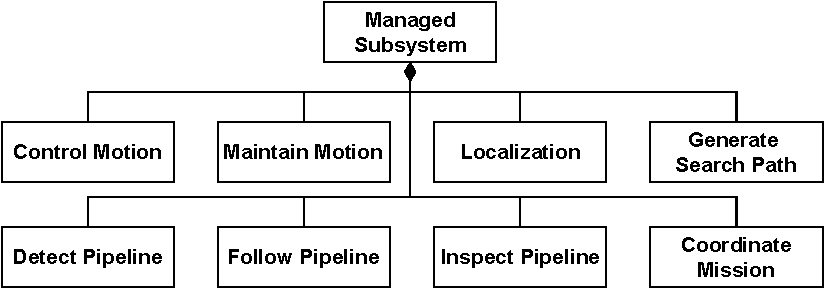
\includegraphics[width=0.8\linewidth]{suave/figures/FunctionalHierarchy.pdf}
    \caption{Managed Subsystem's Functional Hierarchy}
    \label{fig:func_arch}
\end{figure}
%

To overcome the uncertainties $U1$ and $U2$, a managing subsystem
requires the functionalities to \emph{monitor} the environment and the
managed subsystem's internal state, \emph{reason} about it, and
\emph{execute} the managed subsystem's reconfiguration.


\begin{figure}
    \centering
    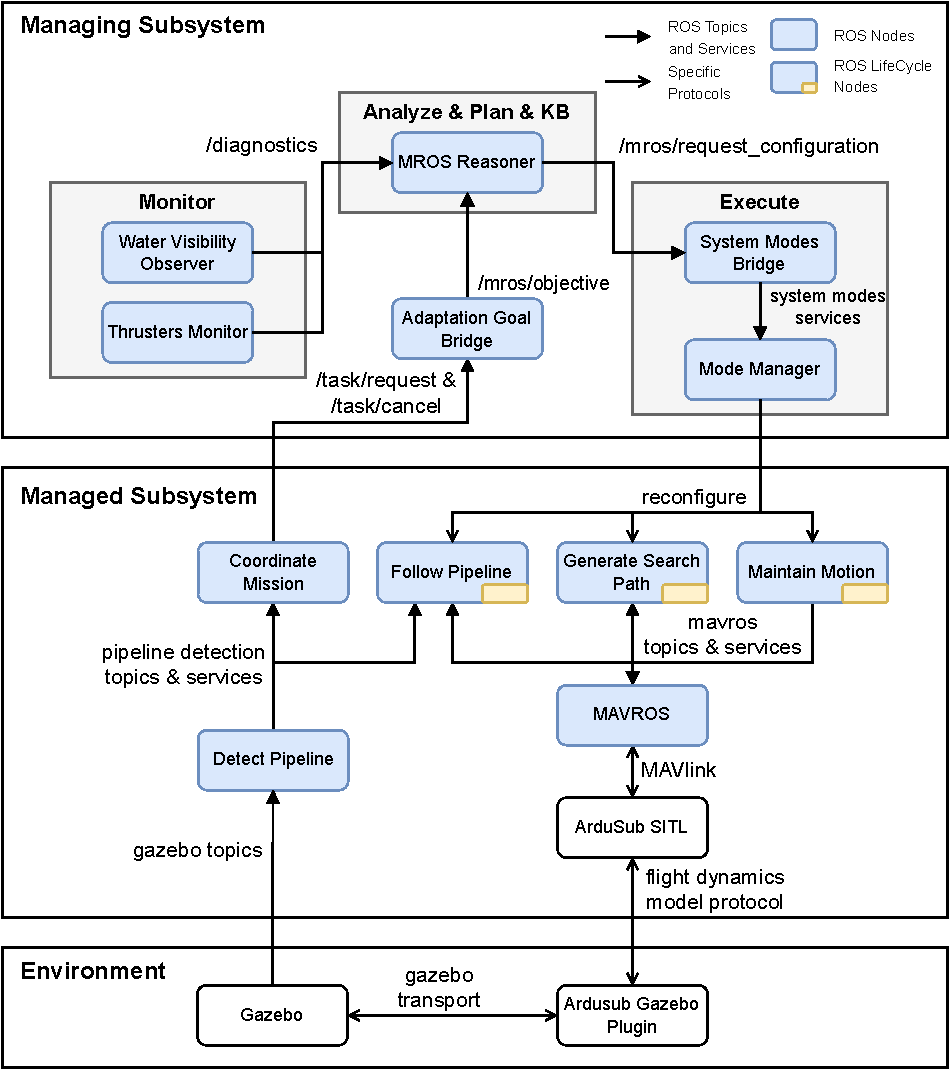
\includegraphics[width=.9\linewidth]{suave/figures/GeneralArchitecture_small.pdf}
    \caption{System Architecture}
    \label{fig:system_architecture}
\end{figure}

The required functions of the managed and managing subsystems
are realized as depicted in Fig.~\ref{fig:system_architecture}. The
managed subsystem is detailed in Section~\ref{sec:managed} and the
managing subsystem in Section~\ref{sec:managing_subsystem}.
It is important to mention that managed subsystem functions
\kw{Control Motion} and \kw{Localization} are achieved by \kw{ArduSub}, and the function \kw{Inspect Pipeline} is not realized since
the actual inspection of the pipeline is not the focus of this
work. It is also important to highlight that this exemplar implements
the function to \emph{reason} about the managing subsystem with Metacontrol to provide a
baseline for future research. However, it can be replaced with other
solutions, as long as they are compatible with the monitor and execute
interfaces, as described in Section~\ref{sec:managing_requirements}.

\section{Managed Subsystem} \label{sec:managed}

The managed subsystem is implemented as a ROS 2-based system and is depicted in Fig.~\ref{fig:system_architecture}. The only non-ROS 2 component is \kw{ArduSub}\footnote{\url{https://www.ardusub.com/}}, which is an open-source autopilot for underwater vehicles. In this application it is used to solve the functions \kw{Control Motion} and \kw{Localization}\footnote{It is assumed that the AUV has appropriate sensors for localization}. The \kw{MAVROS}
package works as a bridge between \kw{ArduSub} and the ROS 2 components. The \kw{Detect Pipeline} node detects the pipeline and informs \kw{Follow Pipeline} and the \kw{Coordinate Mission} node about its position\footnote{A mock perception system is used.}. The \kw{Coordinate Mission} node coordinates the tasks' execution and sets the adaptation goals. Note that the function \kw{Inspect Pipeline} is not implemented,
since the actual inspection of the pipeline is not the focus of this work. However, the exemplar can easily be extended with this functionality by adding a new node that implements the pipeline inspection.

\kw{Follow Pipeline}, \kw{Generate Search Path},  and \kw{Maintain Motion} are lifecycle nodes, which means that they have internal states, such as \emph{active} and \emph{inactive}, and it is possible to switch between these states at runtime. Furthermore, the System Modes package \cite{nordmannSystemModes2021}
extends the state \emph{active} with additional modes, e.g., \emph{active.low\_altitude}.

To adapt the managed subsystem, the managing subsystem adapts the lifecycle nodes by changing their states. This is done by the \kw{Mode Manager} node, which is used off-the-shelf from the System Modes package.
The states available for \kw{Generate Search Path} are \kw{deactivated}, \kw{low altitude}, \kw{medium altitude}, and \kw{high altitude}. Subsequently, the states available for \kw{Follow Pipeline} are \kw{deactivated} and \kw{activated}, while the states for \kw{Maintain Motion} are \kw{deactivated}, and \kw{recover thrusters}.

To enable other developers of self-adaptive systems to use this exemplar and compare different approaches, a \kw{Gazebo}-based  \footnote{\url{https://gazebosim.org/home}} simulation of a pipeline inspection environment and a model of the AUV is provided. The BlueROV2\footnote{\url{https://bluerobotics.com/store/rov/bluerov2/}}
robot was selected as the AUV for the exemplar because (i)~it is compatible with \kw{ArduSub}; (ii)~it is easily integrated with \kw{Gazebo} via plugins; and (iii)~the robot has a low price compared to other available AUVs, making it more accessible to researchers to reproduce the exemplar with a real robot.

\section{Managing Subsystem}
\label{sec:managing_subsystem}

The managing subsystem exploits functional alternatives of the managed
subsystem to enable adaptation and thereby increase system reliability.
Metacontrol is used as an example of how a managing
subsystem can be implemented. This section introduces
Metacontrol
and shows how the adaptation problem can be
formulated and implemented with Metacontrol.

\subsection{Metacontrol Background}
\label{subsec:metacontrol}
\emph{Metacontrol} uses the MAPE-K feedback loop \cite{brun09,kepharTheVision2003} to implement self-adaptation. It \emph{Monitors} the managed subsystem during runtime, \emph{Analyzes} whether the system meets its requirements, \emph{Plans} a new configuration if the system does not meet the requirements, and then \emph{Executes} the reconfiguration of the managed subsystem. All this is done using a shared \emph{Knowledge Base} to which each step refers. In Metacontrol, the knowledge base conforms to the TOMASys (Teleological and Ontological Metamodel for Autonomous Systems) metamodel \cite{corbato2013model}.

\begin{figure}
    \centering
    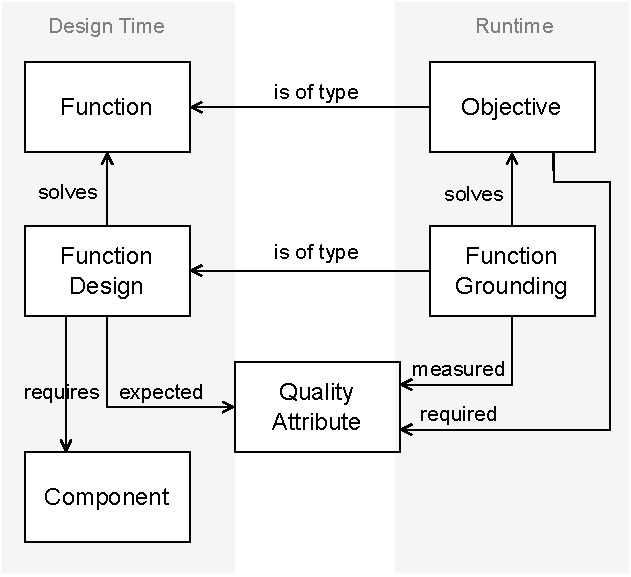
\includegraphics[width=0.6\textwidth]{suave/figures/TOMASys.pdf}
    \caption{A simplified representation of the TOMASys elements}
    \label{fig:tomasys}
\end{figure}

A simplified version of the TOMASys metamodel is displayed in Fig.~\ref{fig:tomasys}.
TOMASys uses \emph{functions} $F$ to represent the functionalities of the system, e.g., generating a search path for the AUV.
The architectural variants that implement these requirements are captured by \emph{function designs} $FD(F, \mathcal{C}, \qa^{exp})$. To distinguish during runtime which function design is most suited in a given situation, a set $\qa^{exp}$ of \emph{expected quality attributes} is associated with it. An expected quality attribute value reflects how well a function design is supposed to fulfill the function $F$ it solves. Furthermore, a function design requires a set $\mathcal{C}$ of \emph{components} of the managed subsystem to solve $F$. A component $C(S_C)$ is a piece of hardware or software, e.g., a sensor or a path-planning algorithm, respectively. The status $S_C$ of a component indicates its availability, i.e., whether it is functioning or not.

An \emph{objective} $O(F,S_O,\qa^{req})$ is a runtime instantiation of a function $F$, e.g., generating a search path with a minimum required water visibility, whose status $S_O$ reflects whether the objective is currently achieved. Furthermore, the set $\qa^{req}$ of \emph{required quality attributes} specifies which quality attribute value the objective requires in order to work properly.

An objective $O$ is solved by a \emph{function grounding} $FG(O,FD,S_{FG}, \qa^{meas})$, which represents the function design $FD$ that is currently used to solve the objective.
Its status $S_{FG}$ reflects whether the function grounding is currently able to achieve the objective. The set $\qa^{meas}$ of \emph{measured quality attributes} reflects how well the function grounding currently fulfills $O$ and is computed using sensor data.


\subsection{Metacontrol Formulation}
\label{sec:metacontrol_formulation}
The functions, architectural variants, and quality attributes required to solve the tasks $(T1)$ Search Pipeline and $(T2)$ Inspect Pipeline, described in Section \ref{sec:problem_statement}, are modeled conforming to the TOMASys metamodel. Table~\ref{tbl:functions_exemplar} specifies the functions ($F_1$)~maintain\_motion, ($F_2$)~generate\_search\_path, and ($F_3$)~follow\_pipeline, while Table~\ref{tbl:qas_exemplar} describes the quality attributes ($QA_1$)~water\_visibility, and ($QA_2$)~performance.
Functions $F_1$ and $F_2$ are required to achieve $T1$, whereas $T2$ is achieved by $F_1$ and $F_3$.
The function designs that solve these functions are specified in Table~\ref{tbl:function_designs_exemplar}. The set of required components is empty for function designs $FD_2 - FD_6$ because they do not require any components that are susceptible to adaptation, or used in the reasoning process.

Since the objectives and function groundings are instantiated during runtime, they are not specified here. An objective for function $F_2$ is for example to generate a search path with no required quality attribute, which is defined as $O_2(F_2, \text{\emph{ok}}, \varnothing)$ in the notation introduced above. A possible function grounding for this objective is $FG_2(O_2, FD_4, \text{\emph{ok}}, \{QA_1^{meas}=1.1\})$.


\begin{table}
    \centering
    \caption{The TOMASys functions used for the exemplar}
    \label{tbl:functions_exemplar}
    \begin{tabular}{|@{\;}l@{\;}|@{\;}l@{\:}|p{4.7cm}@{\:}|}
        \hline
        \textbf{Function} & \textbf{Name} & \textbf{Requirement} \\
        \hline
        \rule{0pt}{2ex}
        $F_1$ & maintain\_motion & Maintain the motion of the robot\\
        \hline
        \rule{0pt}{2ex}
        $F_2$ & generate\_search\_path & Generate a path to search for the pipeline\\
        \hline
        \rule{0pt}{2ex}
        $F_3$ & follow\_pipeline & Follow and inspect the pipeline\\
        \hline
    \end{tabular}
\bigskip
\caption{The TOMASys quality attributes used for the exemplar}
    \label{tbl:qas_exemplar}
    \begin{tabular}{|l|l|l|p{3.9cm}|}
        \hline
        \rule{0pt}{2ex}
        \textbf{QA} & \textbf{Name} & \textbf{Unit} & \textbf{Description}\\
        \hline
        \rule{0pt}{2ex}
        $QA_1$ & water\_visibility & [$0,\infty)$ & Reflects the maximum altitude (in meters) from which the AUV can perceive the seabed\\
        \hline
        \rule{0pt}{2ex}
        $QA_2$ & performance & $[0,1]$ & Reflects how efficient the current search strategy is\\
        \hline
    \end{tabular}
\bigskip
\caption{The TOMASys function designs used for the exemplar}
    \label{tbl:function_designs_exemplar}
    \begin{tabular}{|@{\;}p{3.5cm}@{\;\,}|@{\;}p{3.0cm}@{\,}|p{2.7cm}@{\;}|}
        \hline
        \textbf{Function Design} & \textbf{Name} & \textbf{Description} \\
        \hline
        \rule{-3pt}{2ex}
        $FD_1(F_1,\{\text{thruster}\_x\mid x=1,\dots,6\}, \{QA_2^{exp}=1\})$ & all\_thrusters & Uses all thrusters \\
        \hline
        \rule{-3pt}{2ex}
        $FD_2(F_1, \varnothing, \{QA_2^{exp}=0.5\})$ & recover\_thrusters & Recovers the thrusters that are in failure\\
        \hline
        \rule{-3pt}{2ex}
        $FD_3(F_2, \varnothing, \{QA_1^{exp}=0.5,$ $ QA_2^{exp}=0.25\})$ & spiral\_low & Produces a spiral search path with low altitude \\
        \hline
        \rule{-3pt}{2ex}
        $FD_4(F_2, \varnothing, \{QA_1^{exp}=1,$ $ QA_2^{exp}=0.5\})$ & spiral\_medium & Produces a spiral search path with medium altitude \\
        \hline
        \rule{-3pt}{2ex}
        $FD_5(F_2, \varnothing, \{QA_1^{exp}=2,$ $ QA_2^{exp}=1\})$ & spiral\_high & Produces a spiral search path with high altitude \\
        \hline
        \rule{-3pt}{2ex}
        $FD_6(F_3, \varnothing, \varnothing)$ & follow\_pipeline & Follows the pipeline \\
        \hline
    \end{tabular}
\end{table}

The MAPE-K loop steps in this exemplar are formulated as follows. The monitor step is responsible for measuring $QA_1^{meas}$ and for monitoring the state of the six thrusters.

The analyze step uses Horn rules
to reason about the knowledge base. One example rule that analyzes whether the measured water visibility $QA_1^{meas}$ still satisfies the expected water visibility $QA_1^{exp}$ of the grounded function design is displayed in Fig.~\ref{fig:swrl_rule}. Note that it is written in terms of the notation introduced in Section~\ref{subsec:metacontrol}. Line~\ref{eq:fg} expresses that the rule reasons about a function grounding $FG$ that solves an objective $O$, is of type $FD$, has a status $S_{FG}$ and an associated set of measured quality attributes $\qa^{meas}$. Furthermore, the function design $FD$ solves the function $F$, has a set of required components $\mathcal{C}$ and an associated set of expected quality attributes $\qa^{exp}$. Note that it is implicitly assumed that $FG$ is well-formed, i.e., that the function of which $O$ is a type of is the same as the function that $FD$ solves. Since this rule should analyze the water visibility, Line~\ref{eq:qas_contained} ensures that $QA_1^{meas}$ is an element of the set $\qa^{meas}$ and that $QA_1^{exp}$ is an element of the set $\qa^{exp}$, i.e., that both $FG$ and $FD$ are related to water visibility. Finally, if the measured value of $QA_1$ is less than its expected value associated with the grounded function design, see Line \ref{eq:meas_less_exp}, then the status of the function grounding is set to \emph{error}, see Line~\ref{eq:status_error}.

\begin{figure}[t]
    \centering
    \begin{align}
    &FG\bigl(O, FD, S_{FG}, \qa^{meas}\bigr) \boldsymbol{\wedge} ~ FD(F, \mathcal{C}, \qa^{exp}) \label{eq:fg}\\
    %&\boldsymbol{\wedge} ~ F = G \label{eq:same_function}\\
    & \boldsymbol{\wedge} ~ QA_1^{meas} \in \qa^{meas}
    ~\boldsymbol{\wedge} ~ QA_1^{exp} \in \qa^{exp} \label{eq:qas_contained}\\
    &\boldsymbol{\wedge} ~ QA_1^{meas} < QA_1^{exp} \label{eq:meas_less_exp}\\
    &\boldsymbol{\Rightarrow} ~ S_{FG} = \text{\emph{error}} \label{eq:status_error}
\end{align}
\caption{Rule to analyze whether the measured water visibility $QA_1^{meas}$ still satisfies the expected water visibility $QA_1^{exp}$ of the grounded function design}
\label{fig:swrl_rule}
\end{figure}

In the planning step, the function designs with $QA_1^{exp}$ higher than $QA_1^{meas}$ are filtered out as the visibility they would expect is not measured, afterward the remaining function design with the highest expected search performance ($QA_2^{exp}$) is selected as the desired configuration. The selected configuration is then carried out in the execute step.

\subsection{Metacontrol Implementation}

As depicted in Fig.~\ref{fig:system_architecture}, the monitor step is implemented with the \kw{Water Visibility Observer} and the \kw{Thruster Monitor} nodes. They are used for measuring $QA_1$ and monitoring the status of the six thrusters $\text{thruster}\_x$ where $x\in\{1,\dots,6\}$, respectively.
To simplify the system and avoid the addition of unnecessary nodes, instead of adding water visibility to the Gazebo simulator, the \kw{Water Visibility Observer} simulates water visibility measurements with a sine function, and instead of probing the managed subsystem to identify thruster failures the \kw{Thruster Monitor} simulates the thruster failures events. Since the monitor step is mocked up, and its probes and intermediary nodes that would be required to provide the probes are not implemented, they are not included in Fig. \ref{fig:system_architecture}. Both nodes publish their data into the \kw{/diagnostics} topic with the ROS 2 default \kw{DiagnosticArray} message type.


The knowledge base (KB), the analyze and plan step are implemented using MROS~\footnote{\url{https://github.com/meta-control/mc_mros_reasoner}}~\cite{bozhinoski2022mros}, a ROS 2-based Metacontrol implementation, as the \kw{MROS Reasoner} node. The KB
is implemented with the Ontology Web Language (OWL)~\cite{Antoniou2004}, the Horn rules used for the analyze step with the Semantic Web Rule Language (SWRL)~\cite{horrocks2004swrl}, and the reasoning is done with Pellet\footnote{\url{https://github.com/stardog-union/pellet}}. The \kw{MROS Reasoner} receives water visibility measurements ($QA_1^{meas}$) and thruster status information from the monitor step, then decides whether adaptation is required, and, in this case, selects a desired configuration which it sends to the execute step (see Section \ref{sec:metacontrol_formulation} for more details). The \kw{MROS Reasoner} initially does not have objectives, so it does not perform adaptation. The adaptation reasoning only starts when the \kw{Coordinate Mission} node sends new objectives, such as $O_2(F_2, null , \varnothing)$, via the \kw{Adaptation Goal Bridge}. New objectives do not have a status yet.

The execute step uses the System Modes' \kw{Mode Manager} to adapt the managed subsystem, and the \kw{System Modes Bridge} bridges the \kw{Mode Manager} with the \kw{MROS Reasoner}. When a reconfiguration is needed, the \kw{MROS Reasoner} requests the new configuration via the \kw{/mros/request\_configuration} service to the \kw{System Modes Bridge}.Then the \kw{System Modes Bridge} forwards the request to the \kw{Mode Manager} using the correct service names, depending on the lifecycle node being adapted. The services used by the \kw{Mode Manager} are listed in Table~\ref{tbl:system_modes_services}, and the available modes are listed in Table~\ref{tbl:system_modes_modes}.


\begin{table}
    \centering
    \caption{Available System Modes' services}
    \label{tbl:system_modes_services}
    \begin{tabular}{|p{4cm}|p{5.4cm}|}
        \hline
        \textbf{Node} & \textbf{Service} \\
        \hline
        f\_generate\_search\_path  & /f\_generate\_search\_path/change\_mode   \\
        \hline
        f\_follow\_pipeline  & /f\_follow\_pipeline/change\_mode   \\
        \hline
        f\_maintain\_motion  & /f\_maintain\_motion/change\_mode   \\
        \hline
    \end{tabular}
    \bigskip
    \caption{Available modes}
    \label{tbl:system_modes_modes}
    \begin{tabular}{|p{4cm}|p{3.0cm}|c|}
        \hline
        \textbf{Node} & \textbf{Mode} & \textbf{Lifecycle state} \\
        \hline
        f\_generate\_search\_path & fd\_spiral\_high   & active               \\
        \hline
        f\_generate\_search\_path & fd\_spiral\_medium   & active             \\
        \hline
        f\_generate\_search\_path & fd\_spiral\_low   & active              \\
        \hline
        f\_generate\_search\_path & fd\_unground   & inactive  \\
        \hline
        f\_follow\_pipeline & fd\_follow\_pipeline   & active  \\
        \hline
        f\_follow\_pipeline & fd\_unground   & inactive  \\
        \hline
        f\_maintain\_motion & fd\_all\_thrusters   & inactive  \\
        \hline
        f\_maintain\_motion & fd\_recover\_thrusters   & active  \\
        \hline
    \end{tabular}
\end{table}


\section{Extending and connecting managing subsystems}\label{sec:managing_requirements}

With the described system implementation, the only Metacontrol-specific nodes of the system are the \kw{MROS Reasoner}, the \kw{System Modes Bridge}, and the \kw{Adaptation Goal Bridge}. All other nodes of the system can be reused with different managing subsystems. The only requirement to connect a managing subsystem to the managed subsystem is to ensure that the managing subsystem adheres to the provided monitor and execute ROS 2 interfaces. As described in the previous section, the monitor interface is the ROS 2 topic \kw{/diagnostics}, and the execute interfaces are listed in Table~\ref{tbl:system_modes_services}. To show that changing the managing subsystem is possible, a managing subsystem that randomly picks a configuration was also implemented.

Since the system is implemented with a modular design, it can be extended with additional functionalities and adaptation scenarios by adding new lifecycle nodes and updating the system modes' configuration file accordingly. The implemented functionalities can be replaced with different implementations as long as they adhere to the same interfaces; e.g., the \kw{Pipeline Detection} node could be replaced by a node that actually performs perception instead of a mock-up.


\section{Evaluation}\label{sec:results}
To evaluate the performance of different managing subsystems using this exemplar, the mission described in Section~\ref{sec:problem_statement} was implemented.
The mission consists of the AUV performing $T1$ and $T2$ while subject to $U1$ and $U2$ until a user-provided time limit  is reached. To evaluate the mission, the following metrics were used: the \emph{search time}, the amount of time elapsed from the beginning of the search until the pipeline is found, and the total \emph{distance inspected} of the pipeline.

To provide a baseline for the exemplar, the mission is performed with two different managing subsystems and with no managing subsystem, using a fixed configuration. The managing subsystems are the Metacontrol-based implementation detailed in Section~\ref{sec:managing_subsystem} and a random managing subsystem that selects configurations arbitrarily.

Since the system is non-deterministic due to characteristics of \kw{Gazebo}, \kw{ArduSub}, and the interaction between them, no run of the simulation is exactly the same. Thus, the mission execution and metrics collection are automated with a runner to allow multiple runs to be easily performed.

This section briefly describes how to configure the exemplar, and the results of running the exemplar. Further details may be found in the exemplar repository.

\subsection{Configuring the exemplar}

In SUAVE, the AUV's mission execution can be varied by changing the parameters of the system. In the \kw{Water Visibility Observer}, the available parameters are the water visibility minimum and maximum values, periodicity, and initial phase shift. In the \kw{Thrusters Monitor}, the available parameter is a list with thruster events indicating which thruster fails and when. In the \kw{Coordinate Mission}, the mission time limit can be set. In the random manager, the adaptation periodicity can be set, and when using no manager, the default states for the lifecycle nodes can be set. In addition, the runner is parametrized with the number of runs to execute, and which managing subsystem to select. All parameters are adjusted using configuration files packaged in the exemplar.

\subsection{Results}
The mission was executed with a time limit of 300 seconds, water visibility  periodicity of 80 seconds, minimum and maximum values of 1.25 and 3.75, no phase shift, and thruster 1 failing after 35 seconds from the start of the mission. The results are shown in Table~\ref{tab:results_m1}. It can be noticed that with the Metacontrol managing subsystem both mean \emph{search time}\footnote{When the pipeline is not found, the time limit is used as the \emph{search time}} is lower, and the \emph{distance inspected} is higher.
This indicates that, in this exemplar, Metacontrol improves the performance of the system, and outperforms the random managing subsystem and the system without a managing subsystem.
In addition, the standard deviation (Std) of the \emph{search time} is lower for Metacontrol, indicating that it is more consistent when searching for the pipeline. The Std of the random manager for the \emph{distance inspected} is lower, however, its mean value is also low, indicating that the random manager is consistent in not inspecting the pipeline.
The results shown can be used as a baseline for comparing different managing subsystems.

\begin{table}[t]
\caption{Mission results}
\label{tab:results_m1}
\resizebox{.8\columnwidth}{!}{%
\begin{tabular}{|l|l|ll|ll|}
\hline
\multirow{2}{*}{\textbf{\begin{tabular}[c]{@{}l@{}}Managing\\ subsystem\end{tabular}}} &
  \multirow{2}{*}{\textbf{\begin{tabular}[c]{@{}l@{}}Number \\ of runs\end{tabular}}} &
  \multicolumn{2}{l|}{\textbf{Search time (s)}} &
  \multicolumn{2}{l|}{\textbf{Distance inspected (m)}} \\ \cline{3-6}
                     &            & \multicolumn{1}{l|}{\textbf{Mean}} & \textbf{Std} & \multicolumn{1}{l|}{\textbf{Mean}} & \textbf{Std} \\ \hline
None                 & 20          & \multicolumn{1}{l|}{187.85}             & 42.40            & \multicolumn{1}{l|}{31.40}             & 13.00            \\ \hline
Random               & 20          & \multicolumn{1}{l|}{180.15}             & 82.05           & \multicolumn{1}{l|}{3.88}             & 3.19            \\ \hline
\textbf{Metacontrol} & \textbf{20} & \multicolumn{1}{l|}{\textbf{106.95}}    & \textbf{39.46}   & \multicolumn{1}{l|}{\textbf{51.15}}    & \textbf{12.01}   \\ \hline
\end{tabular}%
}
\centering
\end{table}

\section{Conclusion}\label{sec:conclusion}

This work describes SUAVE, a ROS 2-based exemplar for self-adaptive underwater vehicles used for pipeline inspection. Due to its modular design, SUAVE enables different managing subsystems to be applied to the system without the need to modify the managed subsystem, the monitor nodes, and the executing mechanism. In addition, the system can be easily extended with new functionalities and adaptation scenarios by adding new nodes. Furthermore, this paper provides a baseline for comparing the performance of different managing subsystems, and it shows that the addition of a Metacontrol-based managing subsystem increases the performance of the system in comparison to not using any managing subsystem or one that chooses configurations arbitrary.


In future work, SUAVE can be extended with: more metrics for a more in-depth evaluation; more tasks (e.g., docking), functionalities (e.g. a de facto perception system), and components (e.g. sonars) for more realistic missions; more adaptation scenarios, e.g., adapting to changes in the water currents, and adapting the thruster configuration matrix when a thruster can not be recovered.













\chapter{ROSA: A knowledge-based solution for robot self-adaptation}\label{rosa}

\begin{abstract}
Autonomous robots must operate in diverse environments and handle multiple tasks despite uncertainties. This creates challenges in designing software architectures and task decision-making algorithms, as different contexts may require distinct task logic and architectural configurations. To address this, robotic systems can be designed as self-adaptive systems capable of adapting their task execution and software architecture at runtime based on their context.
This paper introduces ROSA, a novel knowledge-based framework for RObot Self-Adaptation, which enables task-and-architecture co-adaptation (TACA) in robotic systems. ROSA achieves this by providing a knowledge model that captures all application-specific knowledge required for adaptation and by reasoning over this knowledge at runtime to determine when and how adaptation should occur.
In addition to a conceptual framework, this work provides an open-source ROS 2-based reference implementation of ROSA and evaluates its feasibility and performance in an underwater robotics application. Experimental results highlight ROSA’s advantages in reusability and development effort for designing self-adaptive robotic systems.
\end{abstract}

\blfootnote{This chapter is a verbatim copy of the paper~\cite{rosa}.
\begin{itemize}
    \item \textbf{Gustavo Rezende Silva}, Juliane P{\"a}{\ss}ler, S. Lizeth Tapia Tarifa, Einar Broch Johnsen, and Carlos Hern{\'a}ndez Corbato. ``ROSA: A Knowledge-based Solution for Robot Self-adaptation''. Accepted for publication in the Robotics Software Engineering Journal.
\end{itemize}
}


\newpage

\section{Introduction}

A current challenge in robotics is designing software architectures and task decision-making algorithms that enable robots to autonomously perform multiple tasks in diverse environments while handling internal and environmental uncertainties. This challenge arises because different contexts may demand distinct task logic and architectural configurations. At runtime, certain actions may become unfeasible, requiring the robot to adapt its task execution to ensure mission completion. For example, a robot navigating through an environment might run out of battery during its operation, requiring it to adapt its task execution to include a recharge action. Additionally, actions may require different architectural configurations depending on the context. For example, a navigation action that relies on vision-based localization cannot be executed in environments without lights but could potentially be executed with an alternative architectural configuration that employs a localization strategy based on lidar. This becomes even more challenging when both the robot’s task execution and its architectural configuration need to be adapted. For instance, when a robot runs out of battery while navigating, it must simultaneously adapt its architecture to a configuration that consumes less energy and its task execution to include a recharge action and to navigate along paths that are better suited to the new configuration. To address this challenge, robots can be designed as self-adaptive systems~(SASs) with the ability to perform \emph{task-and-architecture co-adaptation}~(TACA)~\citep{ CAMARASoftwareArchitectureTask2020}, i.e., simultaneously adapt their task execution and software architecture dependently during runtime. This work focuses on proposing a systematic solution for enabling TACA that can be reused with different robotic systems.


A common approach to enable self-adaptation in software systems is to design them as two-layered systems containing a managing and managed subsystem~\citep{weyns2020introduction}, where the managing subsystem monitors and reconfigures the managed subsystem, and the managed subsystem is responsible for the domain logic. This design facilitates the development and maintenance of the system by creating a clear separation between the adaptation and the domain logic. While several solutions have been proposed for solving either architectural~\citep{ALBERTS2025112258} or task adaptation in robotic systems~\citep{carreno2021situation, hamilton2022towards}, there are some works that partially address TACA~\mbox{\citep{park2012task, runtime_variability_lotz, rra_nico, temoto}}, and there are few works that fully address TACA~\citep{braberman2018extended, CAMARASoftwareArchitectureTask2020}.
More critically, to the best of our knowledge, the existing solutions for TACA  require a significant and complex re-programming of the adaptation logic for each different use case, including the creation of multiple models based on different DSLs, hindering the adoption of SAS methods in robotics.

To address the limitations of SAS methods for TACA, this paper proposes to extend traditional robotics architectures with a novel knowledge-based managing subsystem for RObot Self-Adaptation~(ROSA) that promotes reusability, composability, and extensibility. The main novelty of ROSA is its knowledge base~(KB) which captures
knowledge about the actions the robot can perform, the robot's architecture, the relationship between both, and their requirements to answer questions such as ``What actions can the robot perform in situation X?'' and  ``What is the best configuration available for each action in situation Y?'', for example, ``Can the robot perform an inspection action when the battery level is lower than 50\%?'' or ``What is the best software configuration for the inspection action when the visibility is low?''.
This results in a reusable solution for TACA in which all application-specific aspects of the adaptation logic are captured in its KB.

In addition to a conceptual framework, this work provides a reference implementation of ROSA as an open-source framework that can be reused for research on self-adaptive robotic systems.  ROSA is implemented as a ROS~2-based system~\cite{ros2}, leveraging \emph{TypeDB}~\citep{dorn2023type, typeql} for knowledge representation and reasoning, and \emph{behavior trees}~(BT)~\citep{colledanchise2018behavior} as well as \emph{PDDL-based planners}~\citep{pddl} for task decision-making.

The \emph{feasibility} of using ROSA for runtime self-adaptation in robotic systems is demonstrated by applying it to the SUAVE exemplar~\citep{suave}, and its adaptation \emph{performance} is evaluated in comparison to other approaches available in the exemplar. ROSA's \emph{reusability} is demonstrated by using it to model the TACA scenarios described by \cite{braberman2018extended} and \cite{CAMARASoftwareArchitectureTask2020}.
The \emph{development effort} for using ROSA is evaluated by analyzing the number of elements contained in the knowledge models created to solve the aforementioned use cases and comparing it with the size of a BT-based approach used to solve SUAVE. ROSA's \emph{development effort scalability} is demonstrated by showing how ROSA's knowledge model grows with the addition of extra adaptations in a hypothetical scenario.

In summary, the main contributions of this paper are:
\begin{enumerate}
\item a \emph{modular architecture} for self-adaptive robotic systems that extends robotics architectures with a managing subsystem and supports reusability, composability, and extensibility;
\item a \emph{reusable knowledge model} to capture all application-specific aspects of the adaptation logic required for TACA in self-adaptive robotic systems;
\item a reference \emph{open-source implementation} of the framework that can be reused for self-adaptive systems research; and
\item an \emph{experimental evaluation} of ROSA based on simulated robotic self-adaptation scenarios.
\end{enumerate}

The remainder of this paper is organized as follows. \Cref{sec:rosa:example} describes the TACA use case used to exemplify and evaluate this work. \Cref{sec:rosa:related_works} presents related works. \Cref{sec:rosa:architecture} describes how this work proposes to extend robotics architectures with ROSA. \Cref{sec:rosa:kb} details ROSA's KB. \Cref{sec:rosa:realization} describes the proposed reference implementation of ROSA. \Cref{sec:rosa:evaluation} showcases ROSA's evaluation. \Cref{sec:rosa:conclusion} concludes this work and presents future research directions.

\section{Running example}\label{sec:rosa:example}
Throughout this paper, the SUAVE exemplar~\citep{suave} is used as an example to ease the understanding of the proposed solution, and later, it is used to evaluate ROSA.

SUAVE consists of an Autonomous Underwater Vehicle (AUV) used for underwater pipeline inspection. The AUV's mission consists of performing the following actions in sequence: \emph{(A1) searching for the pipeline} and \emph{(A2) simultaneously following and inspecting the pipeline}. When performing its mission, the AUV is subject to two uncertainties: \emph{(U1) thruster failures}, and \emph{(U2) changes in water visibility}. These uncertainties are triggers for parameter and structural adaptation. When \emph{U1} occurs while performing \emph{A1} or \emph{A2}, the AUV activates a functionality to recover its thrusters.
When \emph{U2} happens while performing \emph{A1}, the AUV adapts its search altitude.

To demonstrate TACA, this work extends SUAVE with an \emph{(A3) recharge battery} action and a \emph{(U3) battery level} uncertainty. With these extensions, the AUV's battery level can suddenly drop to a critical level, requiring the AUV to abort the action it is performing \emph{(A1 or A2)} and perform \emph{A3}. In this situation, the AUV needs to perform TACA by adapting its task execution and architecture to perform \emph{A3}.
To better evaluate ROSA by serving as a baseline for comparison, this work extends the SUAVE exemplar with a managing subsystem where the adaptation logic is implemented with BTs, and the AUV's architectural variants as well as the architectural adaptation execution are realized with System Modes~\citep{nordmannSystemModes2021}\footnote{The SUAVE exemplar is already configured to use System Modes}. Furthermore, this work introduces a new \emph{reaction time} metric that represents the time a managing system takes to react to uncertainties and adapt the managed subsystem.

\section{Related work}\label{sec:rosa:related_works}

This work combines principles from self-adaptive systems and knowledge representation and reasoning to design a reusable framework for developing adaptive robotics architectures. \Cref{sec:related_rob_archs} analyzes existing robotics architectures and describes the architectural patterns from robotics architectures adopted in this work. \Cref{sec:related_sars} reviews related research on self-adaptive robotic systems that leverage knowledge representation techniques to promote reusability, as well as studies that consider the relationship between task execution and architectural adaptation. Additionally, it discusses how these works influenced the design of the proposed framework and highlights its distinctions from existing approaches.

\subsection{Robotics Architectures}\label{sec:related_rob_archs}

Numerous approaches have been proposed for programming and designing autonomous robot architectures~\mbox{\citep{Kortenkamp2016}}. In recent years, two main trends have emerged: component-based frameworks and middlewares--among which ROS~\cite{ros2} stands out due to its widespread adoption in academia and industry--and layered architectures \mbox{\citep{barnett2022architectural}}. \mbox{\cite{barnett2022architectural}} reviewed 21 robotics architectures and concluded that most architectures follow a layered pattern, and even those that do not can still have their elements mapped onto a layered architectural structure. Furthermore, they found that all architectures include a bottom functional layer responsible for interacting with the robot's hardware, an upper task decision layer--whose responsibilities vary across architectures--and an arbitrary number of intermediate layers. This work aims to design a reusable solution for TACA that can be integrated into robotics architectures adhering to these architectural patterns. To achieve this, the proposed solution establishes a clear separation between architectural management and task logic, organizing them into distinct layers, or subsystems, as commonly referred to in the self-adaptive systems community.

The LAAS architecture~\mbox{\citep{laas_98}} is an example of a three-layered architecture consisting of a functional layer, an executive, and a decision layer. The functional layer contains the robot's control and perception algorithms. The executive layer receives a task plan from the decision layer and selects functions from the functional layer to realize each action in the task plan. The decision layer includes a planner that generates task plans and a supervisor responsible for monitoring plan execution and triggering replanning when necessary.
More recent examples of layered robot architectures include AEROSTACK~\mbox{\citep{Sanchez-Lopez-2016}}, designed for aerial drone swarms, and SERA~\mbox{\citep{Garcia-2018}}, which is tailored for decentralized and collaborative robots. These architectures build on the layered model but focus on providing domain-specific solutions.

Cognitive architectures~\mbox{\citep{Kotseruba-2018}}, such as CRAM~\mbox{\citep{Beetz-2010, Kazhoyan-2021}}, focus on generating intelligent and flexible behavior by integrating cognitive capabilities such as planning, perception, or reasoning. However, being integral solutions, these works provide a blueprint for the complete robot control system and are not intended for reuse and integration with other methods, thus making it difficult to adapt and customize for specific applications.

\subsection{Self-adaptive robotic systems}\label{sec:related_sars}

Despite advances in self-adaptive robotic systems, fully addressing task and architectural co-adaptation (TACA) with reusable and scalable solutions remains an open challenge. While some studies explore the relationship between task execution and architectural adaptation, only a few explicitly address TACA—and those that do face limitations in reusability and practical applicability in robotics. This work aims to bridge this gap by introducing a knowledge-based framework that can capture the necessary knowledge to solve TACA across different use cases, can be directly applied to robotic systems, and supports modular modifications for incorporating different adaptation strategies.

\mbox{\cite{ALBERTS2025112258}} recently conducted a systematic mapping study\footnote{\mbox{\cite{ALBERTS2025112258}} do not claim that the mapping study is a complete overview of the literature but rather a characterization of the field} on ``robotics software architecture-based self-adaptive systems''~(RSASSs), identifying 37 primary studies on RSASSs published since 2011. Among these, \cite{ALBERTS2025112258} identified that four studies~\citep{park2012task, runtime_variability_lotz, rra_nico, CAMARASoftwareArchitectureTask2020} consider, to varying degrees, the relationship between the tasks a robot performs and architectural adaptation. A non-systematic snowballing of the primary studies identified by \cite{ALBERTS2025112258} revealed two additional studies~\citep{braberman2018extended, temoto} that also explore this relationship.

In the context of knowledge-based methods, \cite{ALBERTS2025112258} identified six studies~\citep{park2012task, stefan_adaptive_runtime_models, graph_based_nico, p20_stefan_ice, p26_darko_jasper, suave} that use knowledge representation techniques to capture knowledge required for the adaptation logic. Among these, \citep{p26_darko_jasper, suave} do not propose solutions for RSASSs but instead demonstrate the application of Metacontrol~\citep{hernandez2018self, bozhinoski2022mros} in different robotics use cases.
While these methods do not address TACA, they provide valuable insights for designing knowledge-based approaches to self-adaptation.

\begin{table}[]
\centering
\caption{Related frameworks for robot self-adaptation. Where A-t-T means ``Architectural state triggers task adaptation'', and T-t-A means ``Task triggers architectural adaptation''.}
\label{tab:related_works}
\resizebox{\textwidth}{!}{%
\begin{tabular}{lllllllll}
\hline
\multicolumn{1}{c}{\multirow{2}{*}{\textbf{Approach}}} &
  \multicolumn{2}{c}{\textbf{\begin{tabular}[c]{@{}c@{}}Architectural \\ adaptation\end{tabular}}} &
  \multicolumn{2}{c}{\textbf{TACA}} &
  \multicolumn{2}{c}{\textbf{Reusability}} &
  \multirow{2}{*}{\textbf{\begin{tabular}[c]{@{}l@{}}Robotics \\ Middleware\end{tabular}}} &
  \multirow{2}{*}{\textbf{\begin{tabular}[c]{@{}l@{}}Applied \\ to robot\end{tabular}}} \\ \cline{2-7}
\multicolumn{1}{c}{} &
  \textbf{Parameter} &
  \textbf{Structural} &
  \textbf{A-t-T} &
  \textbf{T-t-A} &
  \textbf{Conceptual} &
  \textbf{\begin{tabular}[c]{@{}l@{}}Software \\ Available\end{tabular}} &
   &
   \\ \hline
ICE~\citep{p20_stefan_ice}             & No           & Yes          & No           & No           & No           & No           & None           & No                 \\
\cite{graph_based_nico}                & No           & Yes          & No           & No           & No           & No           & None           & Real Robot         \\
Metacontrol~\citep{bozhinoski2022mros} & Yes          & Yes          & No           & No           & Yes          & Yes          & ROS 1\&2       & Real Robot         \\
SHAGE~\citep{park2012task}             & No           & Yes          & No           & Yes          & Partially    & No           & None           & No                 \\
\cite{runtime_variability_lotz}        & No           & Yes          & No           & Yes          & No           & No           & None           & No                 \\
RRA~\citep{rra_nico}                   & Yes          & Yes          & No           & Partially    & Yes          & Yes          & ROS 1          & Simulated          \\
TeMoto~\citep{temoto}                  & Yes          & Yes          & No           & Yes          & Partially    & Yes          & ROS 1          & Real robot         \\
MORPH~\citep{braberman2018extended}    & Yes          & Yes          & Yes          & Yes          & No           & No           & None           & No                 \\
\cite{CAMARASoftwareArchitectureTask2020}     & Yes          & Yes          & Yes          & Yes          & Partially    & No           & ROS 1          & Simulated          \\
\textbf{ROSA}                          & \textbf{Yes} & \textbf{Yes} & \textbf{Yes} & \textbf{Yes} & \textbf{Yes} & \textbf{Yes} & \textbf{ROS 2} & \textbf{Simulated} \\ \hline
\end{tabular}%
}
\end{table}

\cite{park2012task} introduced the SHAGE framework for task-based and resource-aware architecture adaptation in robotic systems. SHAGE partially solves TACA, as it can adapt the robot's architecture at runtime to specifically realize each action in its task plan when it needs to be performed. However, SHAGE does not support task execution adaptation based on the robot's architectural state.
SHAGE promotes reusability by leveraging architectural models and knowledge captured with an ontology to reason about adaptation at runtime. However, to the best of our knowledge, there is no implementation of the SHAGE framework that works with common robotic frameworks. Thus, it is not possible to directly reuse SHAGE.

\mbox{\cite{runtime_variability_lotz}} proposed a method to model operational and quality variability using two distinct domain-specific languages~(DSLs) models. Their work provides a high-level discussion on how these models could be used at runtime to enable architectural adaptation based on the actions executed by the robot. An interesting aspect of their approach is the clear separation between functional and non-functional requirements: one model captures the task deliberation logic, functional requirements, and their variation points, while the other focuses on non-functional requirements and their possible variations.
While this separation of concerns simplifies the modeling process, combining task deliberation with functional requirements reduces reusability. Any change in the task deliberation logic directly impacts the modeling of functional requirements, making the approach less flexible. Additionally, they do not provide sufficient details on how these models are used at runtime, nor do they present an evaluation to demonstrate the feasibility of their approach.

\mbox{\cite{rra_nico}} proposed RRA as a model-based approach for structural, parameter, and connection adaptation in robotic systems. Their method employs six distinct models to capture all the knowledge required for adaptation. These models represent the robot's architecture and its variability, its functionalities and their variability, the mapping between functions and architecture, the required interfaces (i.e., inputs, outputs, and data types) for the adaptation logic, and the adaptation logic itself. RRA  models the dependencies between the tasks a robot can perform and the architectural configurations needed to accomplish them. This is achieved by decomposing each task into multiple functionalities and capturing the available architectural variants for realizing each function. At deployment time, the robot's operator selects a task, and RRA manages only the functionalities required for that task. Although RRA considers the relationship between tasks and architecture to some extent, it cannot be classified as TACA, as this dependence is only accounted for at deployment time. Architectural adaptation occurs based on the selected task rather than dynamically at runtime in response to the individual actions the robot needs to perform. Moreover, RRA does not adapt the task execution based on the robot's architectural state.

\cite{temoto} proposed the TeMoto as a general solution for robotic systems' dynamic task and resource management. TeMoto partially solves TACA, as it can adapt the robot's architecture to realize the actions being performed by the robot. TeMoto does not completely fulfill TACA as it cannot adapt the task execution given the robot's architectural state. TeMoto provides reusable mechanisms for resource management, but reusability is limited since the adaptation logic must be implemented for all managed resources, and the knowledge about the dependencies between actions and architecture are programmatically included in the actions' code.

\cite{braberman2018extended} proposed MORPH as a reference architecture to enable TACA. They showcased on a conceptual level how MORPH can be applied to enable TACA in an unmanned aerial vehicle~(UAV) use case. However, since MORPH is only demonstrated at a conceptual level, it is hard to evaluate the feasibility of applying MORPH to robotic systems at runtime. To the best of our knowledge, there is no framework implementing the complete MORPH architecture. Therefore, it is not possible to directly reuse MORPH.

In the context of TACA, \cite{CAMARASoftwareArchitectureTask2020} developed a method for finding \emph{optimal} task and reconfiguration plans for an autonomous ground vehicle~(AGV) navigating in a graph-like environment. To enable optimal planning within reasonable time limits, their method first reduces the search space by finding all possible reconfiguration plans and then computing the shortest N paths the robot can take to reach its goal. Then, it uses this information along with task-specific models that capture mission quality attributes (e.g., energy consumption, collision probabilities) and a preferred utility to apply model checking and determine an optimal reconfiguration plan for each path. Finally, an optimization function selects the best plan based on a predefined utility function (e.g., minimizing energy consumption, time, or collision probability). Although their approach reduces the planning search space to improve planning time, their experiments show that solving the navigation use case still takes an average of $15.1$ seconds, an impractical duration for robots that frequently need to replan at runtime to handle uncertainties. Additionally, while the approach is model-based, it relies on task-specific model transformations (e.g., converting the map or battery model into PRISM model snippets), which require dedicated implementations for different tasks. This limits the reusability of their approach for different types of tasks, as it requires a considerable amount of development effort.

\cite{graph_based_nico} argue that robots should have access to and exploit software-related knowledge about how they were engineered to support runtime adaptation. They demonstrate how labeled property graphs~(LPGs) can be used to persistently store and compose different domain models specified with domain-specific languages~(DSL) to enable runtime architectural adaptation. Although their approach is interesting, its reusability is limited as it does not define a knowledge model that can be reused for other applications: for each different use case and DSL the roboticist is responsible for creating a translation from the DSL to the corresponding LPG.
% In addition, no tools are provided to support the roboticist in integrating Neo4j with robotic systems.

\mbox{\cite{stefan_adaptive_runtime_models, p20_stefan_ice}} propose ICE as a method for adapting the information processing subsystem in multi-robot systems, specifically by adapting the connections between system components. Their approach uses an ontology to define each component's required inputs and outputs, along with quality-of-service information for each connection. This ontology is then translated into answer set programming (ASP), and an ASP solver determines an optimal configuration. While they conceptually demonstrate how their method could be applied to robots, they do not demonstrate it with a robotic system. Moreover, their approach focuses solely on structural and connection adaptation to maintain the functionality of the information processing subsystem, without considering other subsystems of the robotic system.

\mbox{\cite{hernandez2018self, bozhinoski2022mros}} proposed Metacontrol as a knowledge-based solution for parameter and structural adaptation. Metacontrol leverages the TOMASys~\citep{hernandez2018self} ontology to capture the knowledge required for the adaptation logic and to reason at runtime to decide when and how the system should adapt. Similar to RRA, Metacontrol decomposes the system into functionalities, using TOMASys to represent the robot's functionalities, the architectural variants that implement each functionality, and the non-functional requirements associated with these variants. However, Metacontrol cannot perform TACA as TOMASys does not capture the relationship between the system functionalities and the robot's actions.

In conclusion, existing works that fully address TACA~\mbox{\citep{braberman2018extended, CAMARASoftwareArchitectureTask2020}} face limitations in reusability and practical applicability in robotics. The authors of MORPH~\mbox{\citep{braberman2018extended}} note that no complete system has been developed, and they have not demonstrated its feasibility. While the approach proposed by \mbox{\cite{CAMARASoftwareArchitectureTask2020}} provides the most complete solution to TACA in the literature, it also faces reusability limitations by relying on multiple distinct domain-specific language (DSL) models and requiring task-specific implementations for model transformations. To address these limitations, this work proposes capturing all the knowledge required for adaptation logic in a single knowledge model. This approach requires only one model--conforming to the proposed knowledge model--to be designed for each application. Additionally, an open-source reference implementation of ROSA is provided, enabling researchers to reuse, extend, and build upon the proposed solution.

On the other hand, previous knowledge-based methods for RSASS\citep{ park2012task, stefan_adaptive_runtime_models, p20_stefan_ice, graph_based_nico, hernandez2018self, bozhinoski2022mros} do not capture all knowledge required to enable TACA. They either lack the ability to capture the relationship between the robot's actions and architecture \citep{graph_based_nico, hernandez2018self, bozhinoski2022mros}, or the knowledge required to decide when and how the robotic system should adapt~\mbox{\citep{park2012task}}. Although these works do not capture all the knowledge required for TACA, they are able to capture, to varying degrees, knowledge that supports RSASSs. Thus, this work takes inspiration from them to design ROSA's knowledge model while addressing their limitations. More concretely, ROSA's knowledge model is designed to capture the relationship between the robot's actions and architecture and the knowledge required to decide when and how TACA should be performed.

\section{Architecture}\label{sec:rosa:architecture}
To enable TACA, this paper proposes to extend traditional robotics architectures with ROSA, using it as a managing subsystem for the robotic subsystem~(see \Cref{fig:architecture}). This section first describes the assumptions made about the robotics architecture and the requirements to use it alongside ROSA, and then it details ROSA's architecture.

\begin{figure}[h]
    \centering
    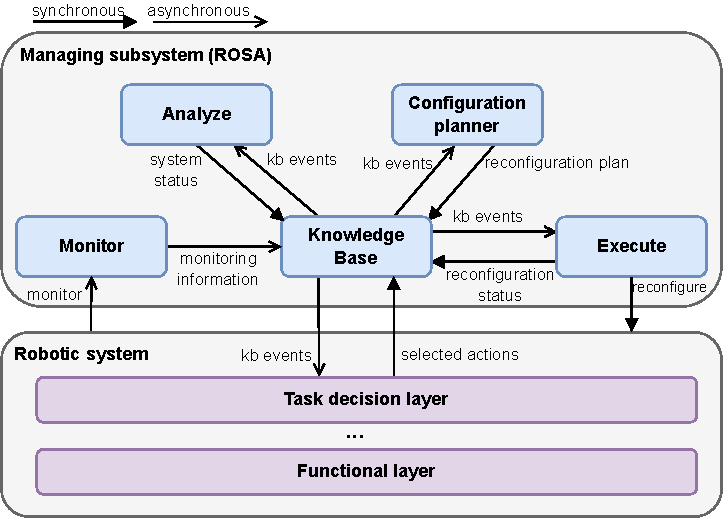
\includegraphics[width=0.5\linewidth]{rosa/figures/system_arch.pdf}
    \caption{The upper layer depicts ROSA's architecture and the bottom layer depicts the robotic system.}
    \label{fig:architecture}
\end{figure}

% \paragraph{Robotic architecture}
\subsection{Robotics architecture}
This work assumes that the robotics architecture is layered, containing a bottom functional layer, an upper task decision layer, and an arbitrary number of layers in between, as common in robotics architectures~\citep{barnett2022architectural}. The functional layer is responsible for interacting with the robots' sensors and actuators, and the task decision layer is responsible for task planning and execution\footnote{Some architecture have distinct layers for handling task planning and execution, in the context of this work, they can be considered as sub-layers of the task decision layer.}. To enable TACA with ROSA, the task decision layer shall use the knowledge contained in ROSA's KB to decide which actions to perform, and it must update the KB with the actions selected to be performed to enable ROSA to configure the robot's architecture accordingly. To enable architectural adaptation, the robotic architecture must be component-based, its components must be able to be activated and deactivated at runtime, and its components' parameters must be able to be adapted at runtime.

% \paragraph{ROSA architecture}
\subsection{ROSA architecture}
ROSA's architecture adheres to the MAPE-K loop~\citep{kepharTheVision2003}. It \emph{monitors} the managed subsystem, \emph{analyzes} whether adaptation is required, when needed, \emph{plans} how the managed subsystem should be reconfigured, and \emph{executes} the selected reconfigurations. All these steps interact with a central \emph{KB}.

To promote reusability, composability, and extensibility, the architecture is designed with the following premises: \emph{(1)} \emph{all} knowledge required for the adaptation logic is captured in the central KB, \emph{(2)} there is no inter-component communication between the MAPE components~\citep{weyns_patterns_2013}, \emph{(3)} the MAPE components insert and read data from or to the KB via standardized interfaces, and \emph{(4)} there is no explicit coordination between the MAPE-K components. Premise \emph{1} promotes reusability by only requiring the modeling of the relevant knowledge for applying ROSA to different applications in a single model. Premises \emph{1} to \emph{4} promote composability and extensibility by allowing the MAPE components to be stateless and self-contained.

\section{Knowledge base}\label{sec:rosa:kb}
To fulfill the architectural premise that all knowledge required for the adaption logic should be captured in a central KB, this work proposes a KB component composed of the knowledge model depicted in  \Cref{fig:k_model} and the set of rules depicted in \Cref{fig:status_diagrams}, described in \Cref{sec:rosa:kb_model} and \Cref{sec:rosa:rules} respectively.

The knowledge model is presented as a conceptual data model conforming to a particular case of the enhanced entity-relationship (EER)\mbox{\cite{herm, thalheim2013entity}} model, an extension of the entity-relationship model \mbox{~\cite{chen1976entity}} that accounts for subclassing and higher-order relationships, i.e., relations between relationships. The EER model captures information as entities, relationships, and attributes. An entity is a ``'thing' which can be distinctly identified''\mbox{~\cite{chen1976entity}}, a relationship is an association among entities or relationships, and an attribute represents a property of an entity or relationship\mbox{~\cite{herm, thalheim2013entity}}. In addition, entities and relationships play a role in the relationships they are part of, which is identified by the label on the arrows in \mbox{\Cref{fig:k_model}}. The rules are also described at a conceptual level as decision diagrams. \mbox{\Cref{sec:rosa:impl}} presents the details on how the knowledge model and rules can be implemented and executed and runtime.


\subsection{Knowledge model}\label{sec:rosa:kb_model}
To enable adaptation, the knowledge model captures
\emph{what} can be adapted with the architectural knowledge depicted in \Cref{fig:arch_model}; \emph{why} to adapt and \emph{how} to select an adaptation with the adaptation heuristics knowledge depicted in \Cref{fig:adapt_model}; and \emph{how} to execute an adaptation with the reconfiguration plan knowledge depicted in \Cref{fig:reconfig_plan}. Tables \ref{tab:elements_km_architectural}-\ref{tab:elements_km_reconfig} define each element in the model alongside examples based on SUAVE to ease its understanding.

\begin{figure}[h]
    \centering
    \begin{minipage}[b]{0.123\textwidth}
        \centering
        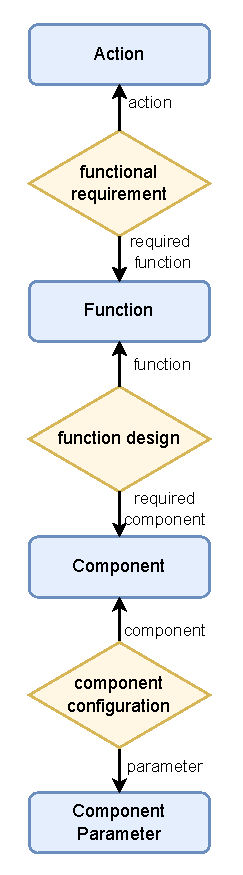
\includegraphics[width=\linewidth]{rosa/figures/arch_k.pdf}
        \caption{Architectural}
        \label{fig:arch_model}
    \end{minipage}
    \hfill
    \begin{minipage}[b]{0.482\textwidth}
        \centering
        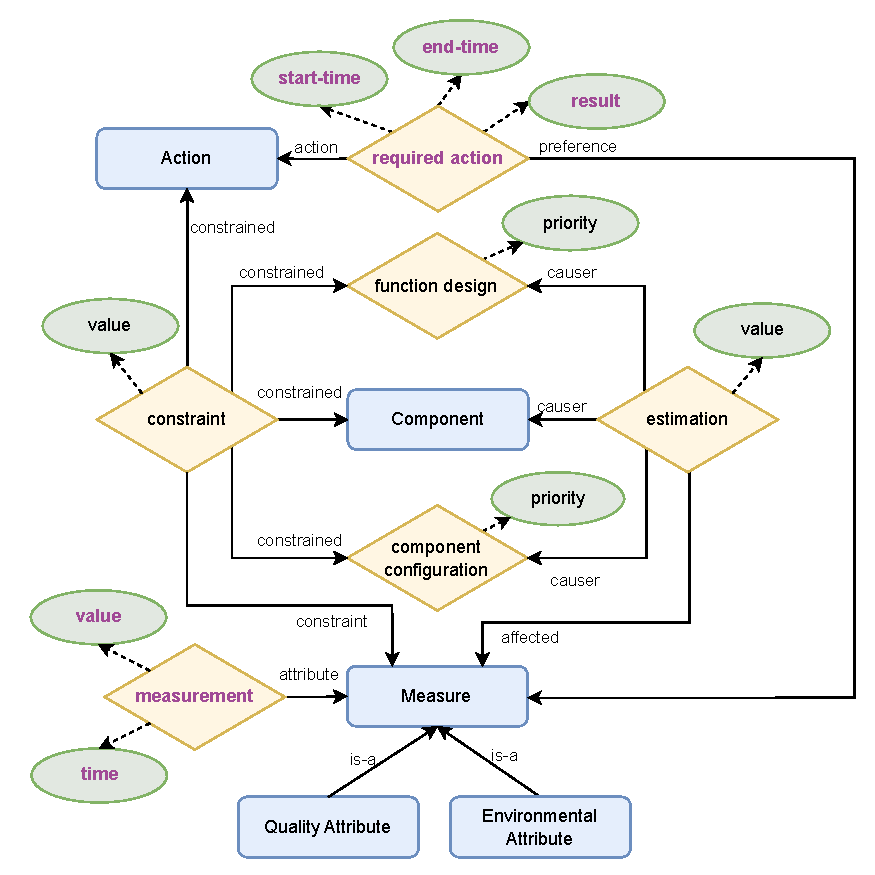
\includegraphics[width=\linewidth]{rosa/figures/adapt_k.pdf}
        \caption{Adaptation heuristic}
        \label{fig:adapt_model}
    \end{minipage}
    \hfill
    \begin{minipage}[b]{0.354\textwidth}
        \centering
        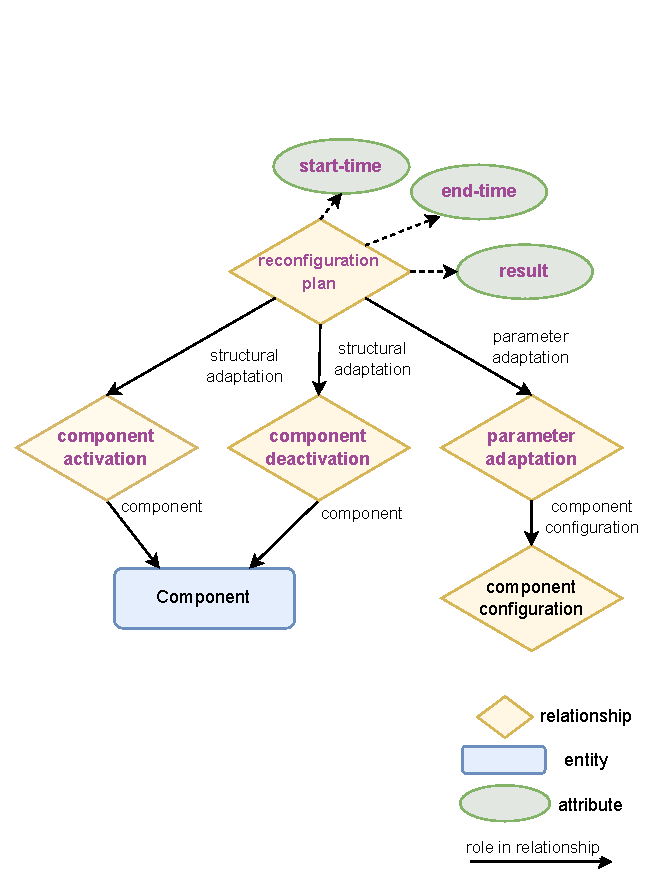
\includegraphics[width=\linewidth]{rosa/figures/reconfig_plan.pdf}
        \caption{Reconfiguration plan}
        \label{fig:reconfig_plan}
    \end{minipage}

    \caption{ROSA's knowledge model. Architectural knowledge is on the left. Adaptation heuristic knowledge in the center. Reconfiguration Plan knowledge on the right. The labels on the arrows represent which role an entity or relationship plays in a relationship. Instances of the entities, relationships, and attributes with \runtimefont are created at runtime. Instances of the other entities, relationships, and attributes are defined at design time.}
    \label{fig:k_model}
\end{figure}

\subsubsection{Architectural knowledge}
The architectural knowledge~(see \Cref{tab:elements_km_architectural}) captures what actions the robot can accomplish, the set of functionalities the robot needs to realize an action, the set of components required to realize a functionality, and the possible parameters for a component.

\begin{table}[h]
\small
\centering
\caption{The elements of the architectural knowledge. Instances of the elements with \runtimefont are created at runtime. Instances of the other elements are defined at design time. The `@key' expression after an attribute indicates that the attribute is used as a unique identifier. E stands for entity and R stands for relationship.}
\label{tab:elements_km_architectural}
\resizebox{\linewidth}{!}{%
\begin{tabular}{p{.01\linewidth}p{.12\linewidth}p{0.3\linewidth}p{0.31\linewidth}p{0.26\linewidth}}
% \begin{tabular}{p{.01\linewidth}p{.09\linewidth}p{0.34\linewidth}p{0.38\linewidth}p{0.18\linewidth}}
\hline
\textbf{} &
  \textbf{Name} &
  \textbf{Definition} &
  \textbf{Example} &
  \textbf{Attributes} \\ \hline
% \multicolumn{5}{l}{\textbf{Architectural knowledge}} \\ \hline
\multirow{4}{*}{E} &
  Action &
  ``Action is defined as an operation applied by an agent or team to affect a change in or maintain either an agent's state(s), the environment, or both.''\citep{ieep1872}. Where in the context of this paper the agent is the robot &
  An AUV can perform the \entity{Action} \instance{search pipeline}, and \instance{inspect pipeline} &
  \attribute{name:String @key}  \attribute{\runtime{status:String}} \attribute{\runtime{is-required:Bool}} \\
 &
  Function &
  ``A function is defined by the transformation of input flows to output flows''~\citep{wiki:sebok}, i.e., a function represents what the system can do &
  An AUV can have several \entity{Functions}, like \instance{generate search path} and \instance{generate path to follow pipeline}. The \instance{generate search path} function can be considered a transformation of the AUV's current position (input) to a goal waypoint (output) &
  \attribute{name:String  @key} \attribute{always-improve:Bool} \attribute{\runtime{status:String}} \attribute{\runtime{is-required:Bool}} \\
 &
  Component &
  Hardware and software parts that compose the system &
  A \instance{thruster} is a hardware component, and a \instance{generate spiral search path node} is a software component &
  \attribute{name:String @key} \attribute{always-improve:Bool} \attribute{\runtime{status:String}} \attribute{\runtime{is-required:Bool}} \attribute{\runtime{is-active:Bool}} \attribute{\runtime{pid:Integer}} \\
 &
  Component \hspace{1cm} Parameter &
  A specific parameter configuration of a \entity{Component} &
  The \instance{generate spiral search path node} component can be configured with different search altitudes. Each search altitude is represented as a distinct \entity{Component Parameter} &
  \attribute{key:String} \attribute{value:String} \\ \hline
\multirow{3}{*}{R} &
  funcional \hspace{1cm} requirement &
  Represents which \entity{Functions} a certain \entity{Action} requires to be performed &
  The \instance{search pipeline} action requires the \instance{control motion}, \instance{maintain motion}, \instance{localization}, \instance{detect pipeline}, \instance{generate search path}, and \instance{coordinate mission} functions &
  N/A \\
 &
  function design  &
  Represents a solution for a \entity{Function} as a set of \entity{Components} \citep{hernandez2018self} &
  The \instance{generate search path} function can have multiple \relationship{function designs}, e.g., one using the \instance{generate spiral search path node} component, and another one using the \instance{generate lawnmower search path node} component &
  \attribute{name:String @key} \attribute{priority:Integer} \attribute{\runtime{status:String}} \attribute{\runtime{is-selected:Bool}} \\
 &
  component configuration &
  Represents a possible configuration of a \entity{Component} as a set of \entity{Component Parameters} &
  The \instance{generate spiral search path node} component can be configured in different ways by combining different values of its search altitude and speed parameters. Each combination is represented as an instance of a \relationship{component configuration} &
  \attribute{name:String @key} \attribute{priority:Integer} \attribute{\runtime{status:String}} \\ \hline
\end{tabular}%
}
\end{table}

The architectural knowledge enables parameter adaptation by capturing each parameter configuration of a component with a distinct \relationship{component configuration} relationship, relating one \entity{Component} to a set of \entity{Component Parameters}. It enables structural adaptation by capturing the different possibilities for solving a system functionality as distinct \relationship{function design} relationships which relate a \entity{Function} to a set of \entity{Components}. It enables TACA by indirectly capturing the dependencies between the robot's actions and architecture with the \relationship{functional requirement} relationship which relates an \entity{Action} to the \entity{Functions} it requires.

At runtime, ROSA performs parameter adaptation by switching the selected \relationship{component configurations}. It performs structural adaptation by changing the selected \relationship{function designs} and consequently the active \entity{Components}. The task decision layer in combination with ROSA performs TACA by selecting suitable \relationship{function designs} and \relationship{component configurations} for each \entity{Action} the robot needs to perform, and with the task decision layer selecting different \entity{Actions} to perform according to the feasible configurations.


\subsubsection{Adaptation heuristic knowledge}
This work considers that the robotic system might need to adapt due to changes in the environment, changes in the system's quality attributes (QAs)~\citep{wiki:sebok}, component failures, and changes in the robot's selected actions.

\begin{table}[h]
\small
\centering
\caption{The elements of the adaptation heuristic knowledge. Instances of the elements with \runtimefont are created at runtime. Instances of the other elements are defined at design time. The `@key' expression after an attribute indicates that the attribute is used as a unique identifier. E stands for entity and R stands for relationship.}
\label{tab:elements_km_heuristic}
\resizebox{\linewidth}{!}{%
\begin{tabular}{p{.01\linewidth}p{.12\linewidth}p{0.3\linewidth}p{0.31\linewidth}p{0.26\linewidth}}
\hline
\textbf{} &
  \textbf{Name} &
  \textbf{Definition} &
  \textbf{Example} &
  \textbf{Attributes} \\ \hline
% \multicolumn{5}{l}{\textbf{Adaptation heuristics knowledge}} \\ \hline
\multirow{3}{*}{E} &
  Measure &
  ``Measure is defined as a function over observations, state variables, and parameters.''\citep{ieep1872}
  &
  An AUV can have the \entity{Measures} \instance{battery level} or \instance{water visibility}&
  \attribute{name:String @key} \\
 &  Quality \hspace{1cm} Attribute &
  Quality Attribute is defined as a function over the system's state variables. Which, according to the Software Engineering Body of Knowledge~\citep{wiki:sebok}, can be considered as ``System functional and non-functional requirements used to evaluate the system performance'' &
  An AUV can have the \entity{Quality Attributes} \instance{battery level}, \instance{battery consumption}, and \instance{safety level} &
  \attribute{name:String @key} \\
 &
  Environmental Attribute &
  Environmental Attribute is defined as a function over observations of the environment. That is, it represents a metric of the environment with respect to a certain attribute &
  An underwater environment can have \instance{water visibility} as an \entity{Environmental Attribute} &
  \attribute{name:String @key} \\ \hline
\multirow{4}{*}{R} &
  \runtime{required action} &
  Represents the \entity{Actions} required at runtime &
  The \instance{inspect pipeline} \entity{Action} can be required to be performed at runtime, leading ROSA to configure the AUV appropriately to carry out the inspection action &
  \attribute{\runtime{start-time:Datetime}} \attribute{\runtime{end-time:Datetime}} \attribute{\runtime{result:String}} \\
 &
  \runtime{measurement} &
  ``Measurement is defined as the act of evaluating the measures''~\citep{ieep1872} &
  The \instance{battery level} \entity{Quality Attributes} can have a measurement of 0.5 &
  \attribute{\runtime{value:Double}} \attribute{\runtime{time:Datetime}} \\
 &
  constraint &
  Represents \entity{Measure} constraints for performing a \entity{Action} or for selecting a \relationship{function design}, \entity{Component}, or \relationship{component configuration} &
  If the \instance{water visibility} environmental attribute is low, the \instance{high altitude} configuration for the \instance{generate spiral search path node} cannot be selected &
  \attribute{operator:String} \attribute{value:Double} \attribute{\runtime{status:String}}  \\
 &
  estimation &
  Represents the estimated impact of a \relationship{function design}, \entity{Component}, or \relationship{component configuration} on a \entity{Measure} &
  A lamp \entity{Component} is expected to positively impact the \instance{water visibility} when turned on &
  \attribute{value:Double} \attribute{type:String} \\ \hline
\end{tabular}%
}
\end{table}

The adaptation heuristic knowledge enables adaptation due to changes in the environment or the system's QAs with the \relationship{constraint} relationship by capturing constraints on the selection of \entity{Actions}, \entity{Components}, \relationship{function designs}, or \relationship{component configurations} in terms of measured values of \entity{Measures}.
It enables adaptation due to component failures by capturing a \entity{Component}'s status as an attribute and adaptation due to changes in the robot's task execution by capturing what \entity{Actions} need to be performed with the \relationship{required action} relationship. At runtime, adaptation is triggered when a measurement violates a constraint, when a component has a failure status, or when required actions change.

To capture the decision criteria on how to select an adaptation, the \attribute{priority} attribute can be used to express the order of priority for selecting each \relationship{function design} or \relationship{component configuration}. For more complex criteria, the \relationship{estimation} relationship can be used to capture the estimated impact of selecting a \relationship{function design}, \entity{Component}, or \relationship{component configuration} on the measured values of \entity{Measures}. Furthermore, a \relationship{required action} can relate to a \entity{Measure} to indicate the preferred \relationship{estimation} when selecting a configuration for that action. At runtime, the configuration planner component exploits this knowledge to decide which configuration to select.


\subsubsection{Reconfiguration plan knowledge}
The reconfiguration plan knowledge represents which component parameters must be updated (i.e., how to execute parameter adaptation) and which components must be activated and deactivated (i.e., how to execute structural adaptation). The execute component exploits this knowledge at runtime to reconfigure the managed subsystem.


\begin{table}[h]
\small
\centering
\caption{The elements of the reconfiguration plan knowledge. Instances of the elements with \runtimefont are created at runtime. Instances of the other elements are defined at design time. R stands for relationship.}
\label{tab:elements_km_reconfig}
\resizebox{\linewidth}{!}{%
\begin{tabular}{p{.01\linewidth}p{.12\linewidth}p{0.3\linewidth}p{0.31\linewidth}p{0.26\linewidth}}
\hline
\textbf{} &
  \textbf{Name} &
  \textbf{Definition} &
  \textbf{Example} &
  \textbf{Attributes} \\ \hline
% \multicolumn{5}{l}{\textbf{Reconfiguration plan knowledge}} \\ \hline
\multirow{4}{*}{R} &
  \runtime{reconfiguration plan} &
  Represents the reconfiguration plan generated in the plan step & When the AUV completes the \instance{search pipeline} action and starts the \instance{inspect pipeline} action, the \relationship{reconfiguration plan} consists of deactivating the \instance{generate spiral search path node} and activating the \instance{follow pipeline node}
   &
  \attribute{\runtime{start-time:Datetime}} \attribute{\runtime{end-time:Datetime}} \attribute{\runtime{result:String}} \\
 &
  \runtime{component activation} &
  Represents the components that should be activated & When the AUV starts the \instance{inspect pipeline} action, the \relationship{component activation} relates to the \instance{follow pipeline node}
   & N/A
   \\
 &
  \runtime{component deactivation} &
  Represents the components that should be deactivated & When the AUV completes the \instance{search pipeline} action, the \relationship{component deactivation} relates to the \instance{generate spiral search path node}
   & N/A
   \\
 &
  \runtime{parameter adaptation} &
  Represents the component parameters that should be updated &
  When the water visibility changes, the \relationship{parameter adaptation} consists of a parameter adaptation of the component configuration of the \instance{generate spiral search path node} & N/A
   \\ \hline
\end{tabular}%
}
\end{table}

\subsection{Rules}\label{sec:rosa:rules}
To enable ROSA to reason about when the managed subsystem should be adapted and what type of adaptation is needed, the KB contains a set of generic rules that define how the status of the system can be inferred based on monitored information, e.g., how to infer if a constraint is violated and how to propagate a constraint violation.
A change in status only occurs when measurements are updated or when a component fails. The complete status inference rules are depicted as decision diagrams in \Cref{fig:status_diagrams}.

The status of the required \entity{Components}, \entity{Functions}, and \entity{Actions} indicate when and what type of adaptation is needed. When a \entity{Component} is ``unsolved'' or in ``configuration error''~(see \Cref{fig:component_status}), parameter adaptation is required, i.e., a new \relationship{component configuration} needs to be selected. When a required \entity{Function} is ``unsolved'' or in ``configuration error''~(see \Cref{fig:function_status}), structural adaptation is required, i.e., a new \relationship{function design} needs to be selected. When a required \entity{Action} is ``unfeasible''~(see \Cref{fig:action_status}), TACA is needed, i.e., the task decision layer must choose a new action to perform, consequently triggering architectural adaptation.

\begin{figure}
    \centering
    \begin{minipage}[b]{0.32\textwidth}
        \centering
        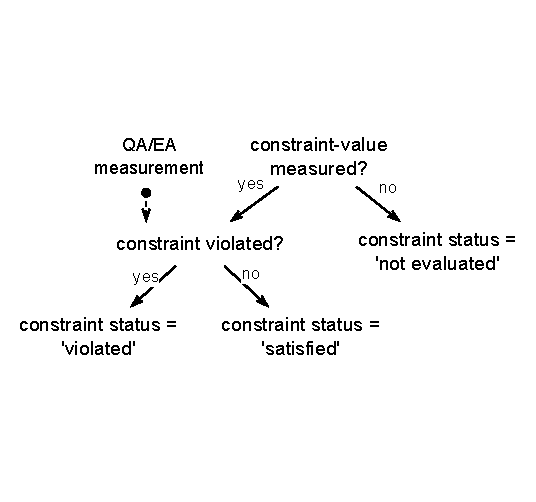
\includegraphics[width=\linewidth]{rosa/figures/constraint_status.pdf}
        \caption{Constraint status}
        \label{fig:constraint_status}
    \end{minipage}
    \hfill
    \begin{minipage}[b]{0.32\textwidth}
        \centering
        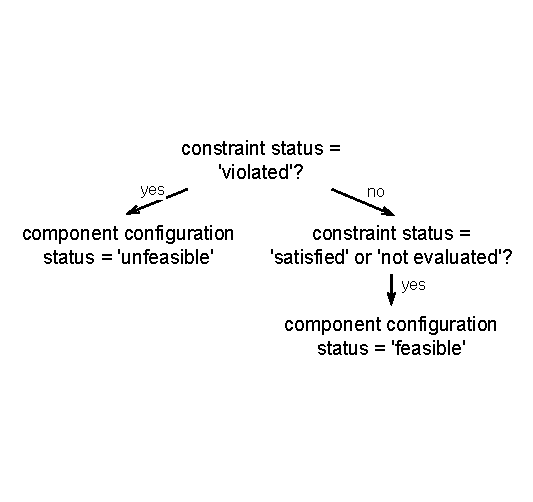
\includegraphics[width=\linewidth]{rosa/figures/component_config_status.pdf}
        \caption{Component configuration status}
        \label{fig:component_config_status}
    \end{minipage}
    \hfill
    \begin{minipage}[b]{0.32\textwidth}
        \centering
        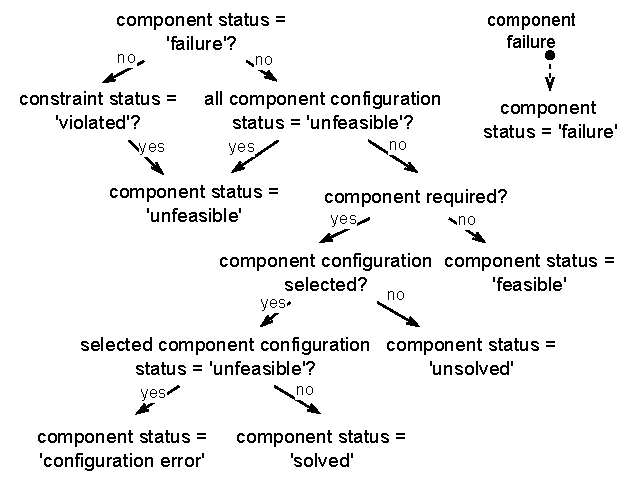
\includegraphics[width=\linewidth]{rosa/figures/component_status.pdf}
        \caption{Component status}
        \label{fig:component_status}
    \end{minipage}

    \vspace{1em}

    \begin{minipage}[b]{0.32\textwidth}
        \centering
        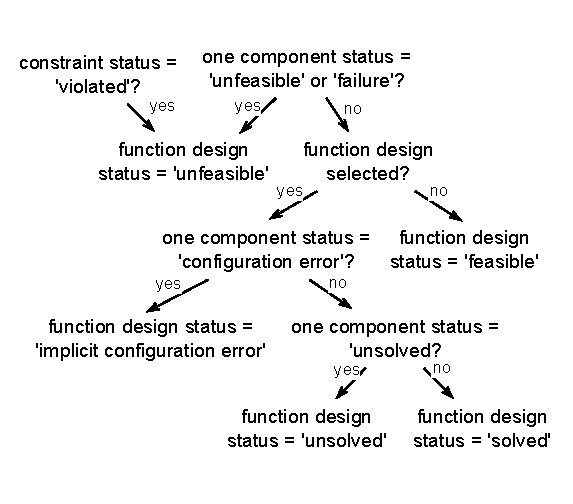
\includegraphics[width=\linewidth]{rosa/figures/function_design_status.pdf}
        \caption{Function design status}
        \label{fig:function_design_status}
    \end{minipage}
    \hfill
    \begin{minipage}[b]{0.32\textwidth}
        \centering
        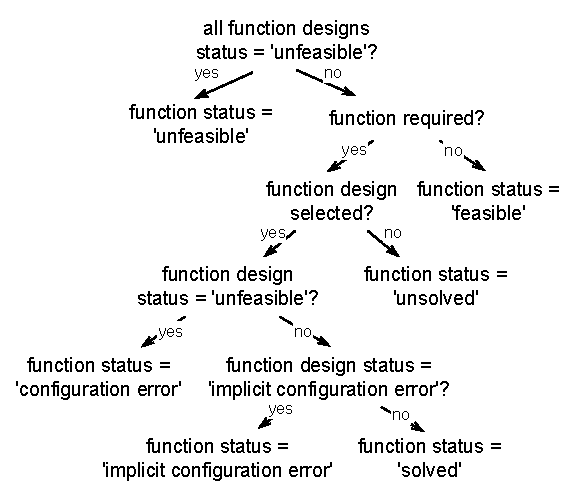
\includegraphics[width=\linewidth]{rosa/figures/function_status.pdf}
        \caption{Function status}
        \label{fig:function_status}
    \end{minipage}
    \hfill
    \begin{minipage}[b]{0.32\textwidth}
        \centering
        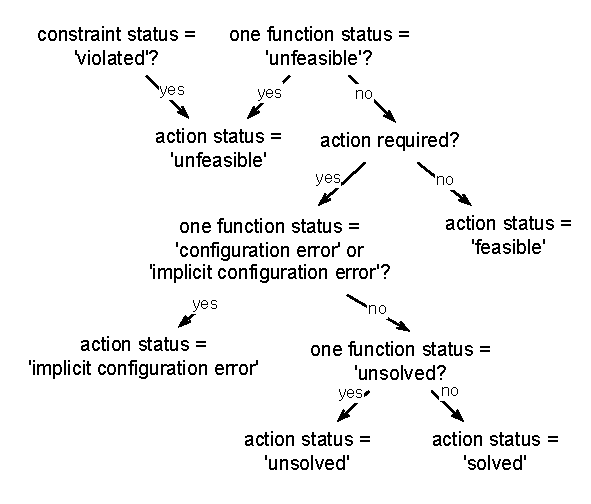
\includegraphics[width=\linewidth]{rosa/figures/task_status.pdf}
        \caption{Action status}
        \label{fig:action_status}
    \end{minipage}

    \caption{Rules used to infer the status of the elements in the knowledge model, presented as decision diagrams.}
    \label{fig:status_diagrams}
\end{figure}

\section{Architecture realization}\label{sec:rosa:realization}
This section details the proposed reference implementation for ROSA. First, the representation requirements imposed by the proposed knowledge model are analyzed to select a suitable knowledge representation technique. Afterward, the proposed implementation is explained.

\subsection{Representation requirements}\label{sec:rosa:rep_req}
The proposed knowledge model was presented as a conceptual data model~(CDM) in a non-machine-readable format. To transform the knowledge model into a machine-readable format while maintaining its semantics and structure, its representation requirements must be identified and used to select a suitable technology to implement it. The representation requirements imposed by the proposed knowledge model are:
\begin{enumerate}
    \item n-ary relationships: the knowledge model contains relationships with different arity\footnote{the number of distinct elements that can be part of a relationship}, e.g., the \relationship{constraint} relationship has arity~5, and the \relationship{measurement} relationship has arity~1;
    \item many-to-many relationships: the knowledge model contains relationships with different cardinalities\footnote{the number of element instances that can be part of a relationship}, e.g., \relationship{function design} is a 1~\entity{Function}-to-many~\entity{Components} relationship;
    \item \label{enum:3} higher-order relationships: some relationships relate relationships to relationships, e.g., the \relationship{constraint} relationship;
    \item \label{enum:4} attributes for entities and relationships: both entities and relationships have attributes, e.g., the \entity{Action} entity and the \relationship{constraint} relationship.
\end{enumerate}


These requirements limit which technology can be used. For example, technologies using graph-based or descriptive logic-based knowledge representation techniques (e.g., OWL~\citep{Antoniou2004}) do not satisfy the representation requirements above apart from allowing attributes for entities (part of Requirement~\ref{enum:4}). Although it is possible to transform the proposed knowledge model into one that can be represented with graph-based or description logic-based approaches by reifying the model~\citep{olive2007conceptual}, each reification applied to the original model can be considered as an introduction of a semantic disparity between the CDM and the machine-readable model, making it harder to understand and reuse it. Thus, this work does not consider applying reification.

A technology that satisfies all representation requirements is TypeDB~\citep{dorn2023type, typeql}. TypeDB is a polymorphic database based on type theory that implements the polymorphic entity-relation-attribute~(PERA)~\cite{typeql} data model. The PERA model subsumes the CDM used as the meta-model for the proposed ROSA model, allowing it to be implemented without modifications. Furthermore, TypeDB has a reasoning system that is able to reason over rules of the form $ antecedent \Rightarrow consequent$ to infer new facts at query time. Where $antecedent$ represents a precondition for inferring the $consequent$ and is expressed as a first-order logic expression combining elements from the model (i.e., entities, relationships, and individuals), and the $consequent$ is a single new fact inferred when the $antecedent$ holds true. The ROSA model rules presented in \Cref{fig:status_diagrams} can be implemented with TypeDB without modifications. For these reasons, this work uses TypeDB to implement the proposed knowledge model and rules.

\subsection{Implementation}\label{sec:rosa:impl}

ROSA is implemented as a ROS 2-based system, where the MAPE-K components~(depicted in \Cref{fig:architecture}) are realized as ROS nodes, and interfaces are implemented using ROS services or topics. The proposed ROSA implementation uses ROS~(Robot Operating System) as its robotics framework since ROS is the current de facto standard robotics framework, and it has been designed, among other things, to promote software reusability in the robotics ecosystem~\cite{ros2}. In this implementation, ROS handles the communication between system components, schedules callbacks for incoming messages and events, and manages the lifecycle of ROS nodes.
The full ROSA implementation is available at \url{https://github.com/kas-lab/rosa}\footnote{In addition to ROSA, this work provides a generic ROS package to integrate ROS~2 with TypeDB: \url{https://github.com/kas-lab/ros_typedb}}.

% \paragraph{Knowledge Base and Analyze}
\subsubsection{Knowledge base and analyze}
The KB component consists of the TypeDB implementation of the proposed knowledge model and inference rules, the ROS interfaces for communicating with the MAPE components, and the logic to manage ROSA's knowledge which is stored in a TypeDB database. In this reference ROSA implementation, TypeDB's reasoner fulfills the role of the analyze component, executing ROSA's inference rules~(\Cref{fig:status_diagrams} to infer new data when the KB is queried. Thus, since TypeDB's reasoner is part of TypeDB, there is no separate analyze component.

\textit{Knowledge model and rules:}
To exemplify how the knowledge model is implemented, \Cref{lst:km} depicts how the \relationship{functional-requirement} relationship and the \entity{Action} entity are defined with TypeQL (TypeDB's query language). Line 1 defines the \relationship{functional-requirement} relationship, and lines 2-3 define that it can relate elements that play the role of \instance{actions} and \instance{required-functions}. Lines 5-7 define the \entity{Action} entity and that it has the attributes `action-name' (its unique identifier) and `action-status'. Lines 8-9 define that it can play the \instance{action} role in a \relationship{functional-requirement} relationship and the \instance{constrained} role in a \relationship{constraint} relationship.

% \begin{figure}
% \vspace{-4ex}
\begin{lstlisting}[caption=TypeQL query to define \relationship{functional-requirement} and \entity{Action}, label=lst:km, columns=fullflexible, language=TypeQL]
functional-requirement sub relation,
  relates action,
  relates required-function;

Action sub entity,
  owns action-name @key,
  owns action-status,
  plays functional-requirement:action,
  plays constraint:constrained;
\end{lstlisting}
% \end{figure}

\Cref{lst:rules} exemplifies how the inference rules are implemented with TypeQL. The \entity{component-status-configuration-error} rule defines that a \entity{Component} has a `configuration error' status when it is required, it does not have an `unfeasible' or `failure' status, and it is in a \relationship{component-configuration} relationship that is selected and has an `unfeasible' status~(see \Cref{fig:component_status}).

% \vspace{-2ex}
% \begin{figure}
% \vspace{-4ex}
\begin{lstlisting}[caption=TypeQL rule to infer whether a component is in `configuration error', label=lst:rules, columns=fullflexible, language=TypeQL]
rule component-status-configuration-error:
 when {
  $c isa Component, has is-required true;
  not {
    $c has status $c_status;
    $c_status like 'unfeasible|failure';
  };
  (component: $c) isa component-configuration,
    has is-selected true,
    has status 'unfeasible';
 } then {
   $c has status 'configuration error';
 };
\end{lstlisting}
% \vspace{-5ex}
% \end{figure}

\textit{Interfaces:}
% \paragraph{Interfaces}
The KB component abstracts the details of interacting with TypeDB with the ROS interfaces it implements, enabling the MAPE components to read and write knowledge via the interfaces described in \Cref{tab:ros_interfaces}.
When the MAPE components request or send data to the KB component via these interfaces, the KB component queries the TypeDB database to retrieve or write knowledge. For example, when the task decision layer calls the service \emph{/action/selectable} to retrieve the name of the selectable \entity{Actions} (i.e., actions that do not have an `unfeasible' status), the KB component performs the TypeQL query depicted in \Cref{lst:typedb_query} to retrieve the name (unique identifiers) of the selectable \entity{Actions}.
When data is written in the KB, the KB component publishes a message in the \emph{/events} topic specifying which type of data was written, i.e., `monitoring data', `action update', `reconfiguration plan'. Additionally, the KB component provides the \emph{/query} service, which can be used to perform \emph{any} TypeDB query to the database. It is not used in ROSA's runtime workflow, but it enables users to perform custom queries, for example, to retrieve all reconfiguration plans that were executed.

\begin{table}[h]
\centering
\caption{ROS interfaces}
\label{tab:ros_interfaces}
\begin{tabular}{lll}
\hline
\multicolumn{3}{l}{\textbf{Topics}} \\ \hline
\textbf{Publisher} &
  \textbf{Subscriber} &
  \textbf{Name} \\ \hline
KB &
  \begin{tabular}[c]{@{}l@{}}Configuration Planner\\ Execute\\ Task Decision Layer\end{tabular} &
  $\sim$/events \\ \hline
Monitor nodes &
  KB &
  /diagnostics \\ \hline
\multicolumn{3}{l}{\textbf{Services}} \\ \hline
\textbf{Server} &
  \textbf{Client} &
  \textbf{Name} \\ \hline
\multirow{4}{*}{KB} &
  Configuration Planner &
  \begin{tabular}[c]{@{}l@{}}$\sim$/function/adaptable\\ $\sim$/function\_designs/selectable\\ $\sim$/function\_designs/priority\\ $\sim$/component/adaptable\\ $\sim$/component\_configuration/selectable\\ $\sim$/component\_configuration/priority\\ $\sim$/select\_configuration\end{tabular} \\ \cline{2-3}
 &
  Execute &
  \begin{tabular}[c]{@{}l@{}}$\sim$/reconfiguration\_plan/get\_latest\\ $\sim$/reconfiguration\_plan/result/set\\ $\sim$/component/active/set\\ $\sim$/component\_parameters/get\end{tabular} \\ \cline{2-3}
 &
  Task Decision Layer &
  \begin{tabular}[c]{@{}l@{}}$\sim$/action/selectable\\ $\sim$/action/request\end{tabular} \\ \cline{2-3}
 &
  User &
  $\sim$/query \\ \hline
\end{tabular}
\end{table}

\begin{figure}
\begin{lstlisting}[caption=TypeDB query to fetch selectable actions' names, label=lst:typedb_query, columns=fullflexible, language=TypeQL]
match  $a isa Action, has name $name;
  not {$a has status 'unfeasible';};
  fetch $name;
\end{lstlisting}
% \vspace{-5ex}
\end{figure}

% \paragraph{Monitor}
\subsubsection{Monitor}
ROSA's implementation does not provide generic monitor nodes. They should be implemented as needed for each application with the requirement that they publish the monitored information in the \emph{/diagnostics} topic\footnote{The \emph{/diagnostics} topic is a standard topic for publishing system diagnosis information within the ROS ecosystem. See \href{https://www.ros.org/reps/rep-0107.html}{ROS REP 107} for more information.} with the standard ROS \emph{DiagnosticArray} message format.
When a monitor node sends measurement updates to the KB, the message field in the \emph{DiagnosticStatus} message needs to be set to `QA measurement' or `EA measurement', and when sending component status updates (e.g., that the component is in failure), the message field must be set to `Component status'. When the KB receives monitoring data, it sends an event message in the `/events' topic to inform that monitoring data was written in the KB.

\subsubsection{Configuration planner}
The configuration planner component selects the configurations (i.e., \relationship{function designs} or \relationship{component configuration}) with the highest priority. When the configuration planner receives an event message indicating that monitoring data was written in the KB or that there was an update in the required actions, it calls the services `/function/adaptable' and `/component/adaptable' to check which \entity{Functions} and \entity{Components} must be adapted. Then, it calls the services `/function/selectable' and `/component/selectable' to check which \relationship{function designs} and \relationship{component configurations} are available for the \entity{Functions} and \entity{Components} that need to be adapted. Finally, the configuration planner selects the \relationship{function designs} and \relationship{component configurations} with the highest priority and informs the KB about the newly selected configuration by calling the service `/select\_configuration'. When this service is called, the KB component checks the current state of the robot, creates a \relationship{reconfiguration plan} to bring the robot to the goal configuration, and sends an event message in the `/events' topic to inform that there is a new reconfiguration plan available.

\subsubsection{Execute}
In ROS-based systems, software components are realized either as ROS nodes or as a particular type of ROS nodes called \emph{lifecycle} nodes. The difference between both is that the latter can be set to different states at runtime, such as \emph{active} and \emph{inactive}, and the former cannot. To enable ROSA to leverage ROS~2 mechanisms to adapt the system, the knowledge model was extended to capture knowledge about ROS~2 components as depicted in \Cref{fig:ros_schema}. The execute component performs structural adaptation by starting or killing ROS nodes or switching the state of lifecycle nodes to active or inactive, and it performs parameter adaptation by calling the ROS's parameter API to change the ROS nodes' parameters at runtime.

\begin{figure}[h]
    \centering
    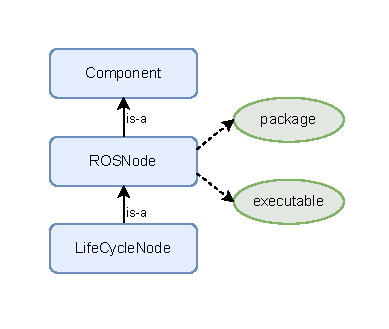
\includegraphics[width=.4\linewidth]{rosa/figures/ros_schema.pdf}
    \caption{ROS specific knowledge}
    \label{fig:ros_schema}
\end{figure}

When the execute component receives an event message indicating that a new reconfiguration plan was added to the KB, it calls the service `/reconfiguration\_plan/get\_latest' to get the latest \relationship{reconfiguration plan}. Then, it adapts the robot's architecture according to the reconfiguration plan. Finally, it calls the services `/reconfiguration\_plan/result/set' and `/component/active/set' to update the KB with the result of the reconfiguration plan and which components are active.

% \paragraph{Task planner}
\subsubsection{Task decision layer}
ROSA's implementation provides an integration for the task decision layer for both PDDL-based planners and BTs, which are implemented leveraging the PlanSys2~\citep{plansys2} and the BehaviorTree.CPP\footnote{\url{https://www.behaviortree.dev/}} packages, respectively.


\emph{Planning:}
To enable task decision-making and execution with PDDL-based planners in combination with ROSA, the planner and plan executor must consider the runtime feasibility of performing the robot's actions as inferred by the KB component.
This work maps the action status from ROSA's knowledge model to PDDL by
capturing whether the action's status is feasible as a PDDL predicate of the form ``\emph{action\_feasible ?action}'' and using it as a precondition to select the respective action. An example can be seen in~\Cref{lst:task_interface_pddl} where the action \emph{my\_action} can only be selected when it does not have an `unfeasible' status in the KB.
At runtime, if an action becomes unfeasible during execution, the plan executor triggers re-planning to generate a new action plan. This results in task execution adaptation and, if the newly selected actions require a different architectural configuration, also in architectural adaptation, i.e., TACA.

\begin{lstlisting}[caption=PDDL formulation example for ROSA, label=lst:task_interface_pddl, columns=fullflexible, language=PDDL]
 (:durative-action my_action
   :parameters (?a - action ...)
   :duration (...)
   :condition (and
     (over all (my_action_action ?a))
     (over all (action_feasible ?a))
     ...
   )
   :effect (and ...)
 )
\end{lstlisting}
% \vspace{-5ex}
% \end{figure}

To handle the interaction between PlanSys2 and ROSA's KB, this work provides a custom ROS~2 node called \emph{RosaPlanner} and a custom PlanSys2 action called \emph{RosaAction}. The \emph{RosaPlanner} is responsible for querying the KB and updating the PDDL problem formulation with information on whether the ROSA actions are feasible or not using the aforementioned ``\emph{action\_feasible ?action}'' PDDL predicate. The \emph{RosaAction} action is responsible
for querying the KB to request or cancel an \entity{Action} when the execution of an action starts or finishes. Each PlanSys2 action that should be managed by ROSA should derive from \emph{RosaAction}, and it should implement the logic for the specific action execution.

\emph{Behavior trees:}
% \paragraph{Behavior trees}
To enable task decision-making and execution with BTs in combination with ROSA, the BTs must consider the runtime feasibility of performing the robot's actions as inferred by the KB component. This work proposes adding before action nodes a condition node that queries the KB to ask whether the following action is feasible. The proposed pattern is depicted in \Cref{fig:tasK_interface_bt}, where the action \emph{MyAction} would only be executed when its status in the KB is not `unfeasible'.

To enable the use of the BehaviorTree.CPP package to implement BTs for ROSA and abstract away the interactions with the KB, this work implements a reusable custom condition node called \emph{IsActionFeasible} and a custom action node called \emph{RosaAction}. The condition node queries the KB to check whether an \entity{Action} is feasible before selecting it to be executed, and the action node queries the KB to request or cancel an \entity{Action} when the execution of an action starts or finishes, respectively.

\begin{figure}[h]
    \centering
    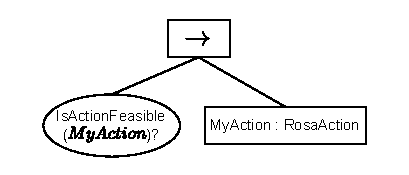
\includegraphics[width=0.5\linewidth]{rosa/figures/task_interface_bt.pdf}
    \caption{BT pattern for TACA with ROSA. The \emph{IsActionFeasible} condition node takes the action name as a parameter. The \emph{MyAction} node derives from the proposed \emph{RosaAction} node and implements the action execution. The action names in the BT must match the names defined in the KB.}
    \label{fig:tasK_interface_bt}
\end{figure}


\section{Evaluation}\label{sec:rosa:evaluation}

This section evaluates ROSA to answer the following questions:
\begin{itemize}
    \item \emph{Feasibility}: Is it feasible to use ROSA to enable runtime TACA in ROS 2-based robotic systems?
    \item \emph{Performance}: How does ROSA perform compared to other managing subsystems for ROS 2-based systems?
    \item \emph{Reusability}:  To what extent can ROSA's knowledge model capture the knowledge required for TACA?
    \item \emph{Development effort}: What is the development effort of using ROSA for adding adaptation to different robotic systems and how does it compare to other approaches?
    \item \emph{Development effort scalability}: How does the development effort of using ROSA for adding adaptation to robotic systems scale for more complex systems?
\end{itemize}

\subsection{Experimental design}

\subsubsection{Feasibility} To evaluate the feasibility of applying ROSA at runtime to enable TACA in ROS~2-based robotic systems, it was applied to the SUAVE exemplar described in \Cref{sec:rosa:example}. SUAVE was selected since, to the best of our knowledge, it is the only ROS~2-based open-source exemplar for self-adaptive robotic systems.

\subsubsection{Performance}
To evaluate ROSA's performance, metrics were collected
with the SUAVE exemplar.
The metrics collected were the ones available in SUAVE, \emph{search time} and \emph{distance of the pipeline inspected}, in addition to the \emph{reaction time} metric introduced in this paper. For the original use case, the experiments were performed with no managing subsystem, with a BT managing system, with Metacontrol\footnote{Metacontrol is the only managing subsystem packaged with SUAVE. The Metacontrol implementation for this use case is described in detail in the SUAVE paper~\citep{suave}.}, and with ROSA. For the extended use case, the experiments were performed with a BT managing system and with ROSA.


\subsubsection{Reusability}
To evaluate to what extent ROSA's knowledge model can capture the knowledge required for TACA, it was used to model the TACA scenarios presented by ~\cite{CAMARASoftwareArchitectureTask2020} and ~\cite{braberman2018extended}\footnote{To the best of our knowledge, these are the only two scenarios in the literature in which the authors explicitly claim the need for TACA.}, and we showcase how the captured knowledge can be exploited to enable TACA. The experimental setup for both scenarios is not publicly available. Thus, it was not possible to apply ROSA at runtime to the simulated environments they used.

\subsubsection{Development effort} To evaluate the development effort of using ROSA to enable adaptation in robotic systems, we analyze the number of elements contained in the ROSA model created to solve the use cases described in this paper. Furthermore, we compare it to the number of elements modeled with the BT approach to solve the SUAVE use case.

\subsubsection{Development effort scalability} To analyze how ROSA's development effort scales for more complex use cases, we showcase how many elements must be modeled in ROSA's model to include structural and parameter adaptation in a hypothetical adaptation scenario.

\medskip

The experimental setup for the \emph{Feasibility} and \emph{Performance} evaluation is open source and reproducible, it can be found at
\url{https://github.com/kas-lab/suave_rosa}.
The models designed to evaluate \emph{Reusability} can be found at
\url{https://github.com/kas-lab/rosa_examples}.

\subsection{Feasibility}
% \paragraph{Knowledge model}
\subsubsection{Experimental setup}
To solve the adaptation scenarios of the SUAVE exemplar with ROSA, the model depicted in \Cref{fig:suave_rosa_model} was created.

\begin{figure*}[h]
    \centering
    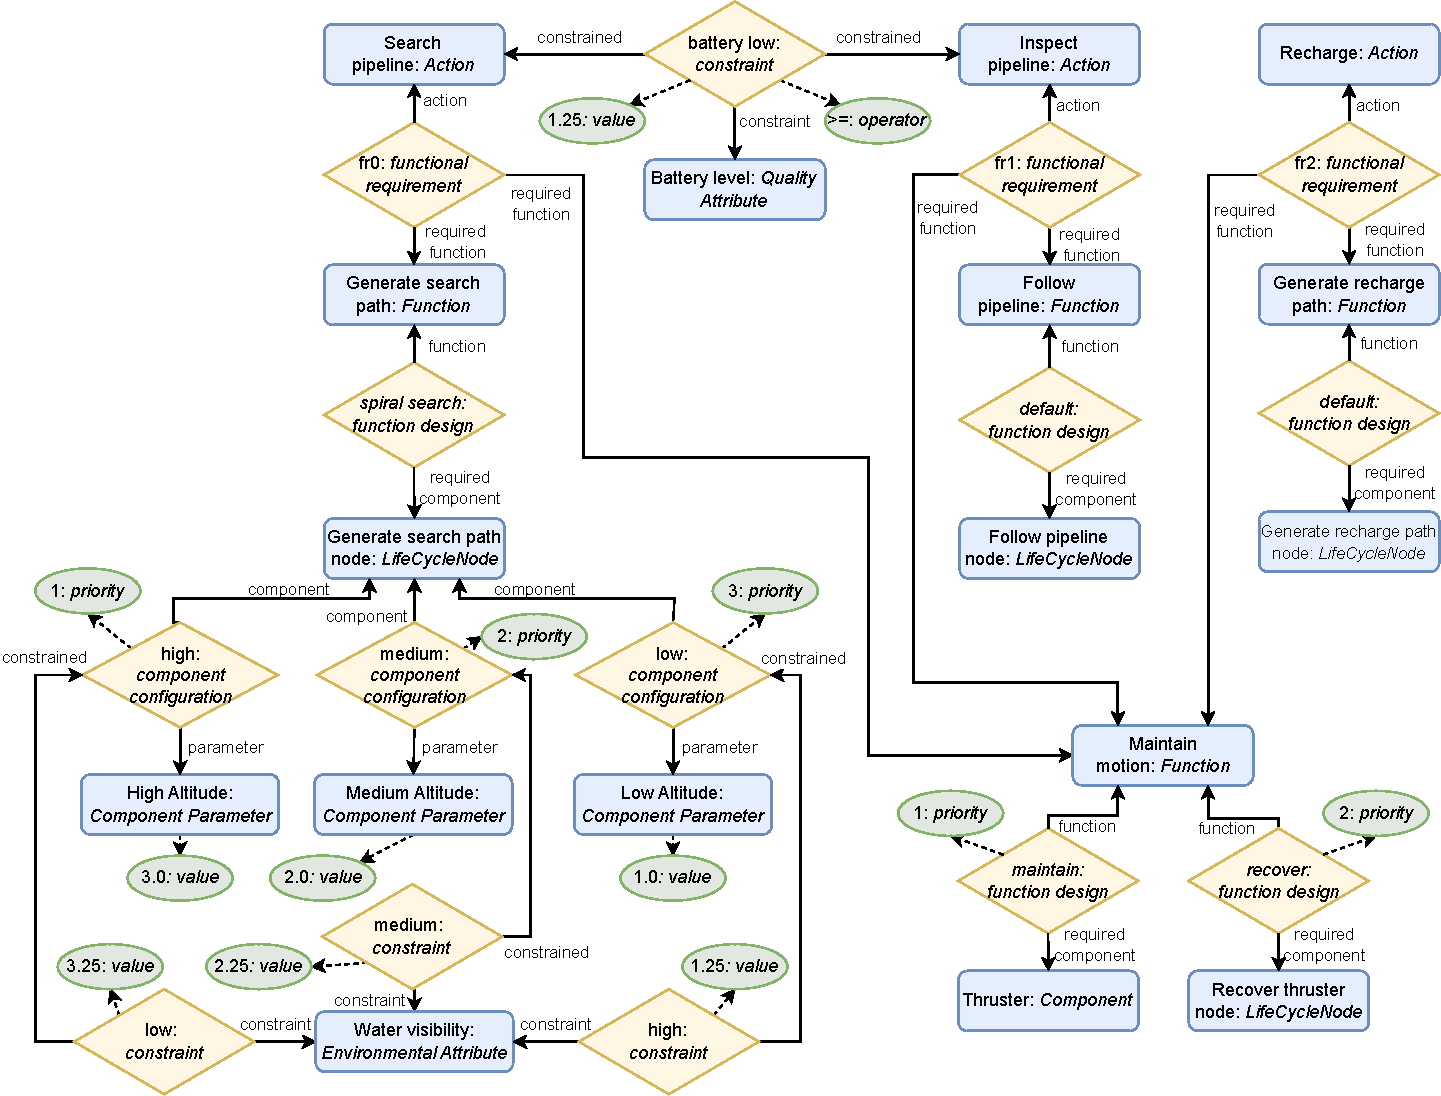
\includegraphics[width=.85\linewidth]{rosa/figures/knowledge_model_suave.pdf}
    \caption{ROSA model for SUAVE.}
    \label{fig:suave_rosa_model}
\end{figure*}

\textit{Thruster failure}~($U_1$) was solved with structural adaptation by including two possible \relationship{function designs} of the \instance{maintain motion} function.
\textit{Runtime behavior:} when a thruster fails, the \instance{maintain} function design status is set to unfeasible (see \Cref{fig:function_design_status}), and it cannot be selected anymore. Then, the \instance{recover} function design is selected, and the \instance{recover thruster node} component is activated. If all thrusters are recovered, the \instance{maintain} function design status becomes feasible and is selected again.

\textit{Changing water visibility}~($U_2$) was addressed with parameter adaptation by including three \relationship{component configurations} for the \instance{generate spiral node}, each representing a different altitude for searching for the pipeline. Furthermore, a \instance{water visibility} \relationship{constraint} was added to each configuration, representing the minimum water visibility in which the configuration can be used. \textit{Runtime behavior:} if the measured water visibility is higher than $3.25$, the component configuration \instance{High} is selected since it has priority number one. If the water visibility drops below $3.25$, its constraint status is set to violated (see \Cref{fig:constraint_status}), and, consequently, its status is set to unfeasible (see \Cref{fig:component_config_status}). Depending on the water visibility, the component configuration \instance{Medium} or \instance{Low} is then selected. If the water visibility increases again above $3.25$, the \instance{High} component configuration status becomes feasible and is selected.

\textit{Critical battery level}~($U_3$), occurring only in the extended SUAVE use case, was solved with TACA by extending the knowledge model with a \instance{recharge} action, and a \instance{battery level} \relationship{constraint} to the \instance{search pipeline} and \instance{inspect pipeline} actions, representing the minimum battery level at which they can be selected.
\textit{Runtime behavior:} when the battery level drops below $0.25$, the status of both the \instance{search pipeline} and \instance{inspect pipeline} actions is set to unfeasible, and the task decision layer cannot select them anymore. Therefore, the task decision layer selects the \instance{recharge} action which also triggers structural adaptation.

Note that extending the solution to solve SUAVE's extended version only required the inclusion of additional knowledge of the \instance{recharge} action and the \relationship{constraint} to the \instance{search pipeline} and \instance{inspect pipeline} actions. This demonstrates that an existing application modeled with ROSA can easily be extended to solve additional adaptation scenarios.

To apply ROSA in simulation to the SUAVE exemplar, the knowledge model depicted in \Cref{fig:suave_rosa_model} was implemented with TypeDB (see an example in \Cref{lst:suave}), and the AUV's mission was implemented with the BT depicted in \Cref{fig:bt_extended} as well with the PDDL formulation partially shown in \Cref{lst:suave_extended_pddl}.

\begin{figure}[h]
    \centering
    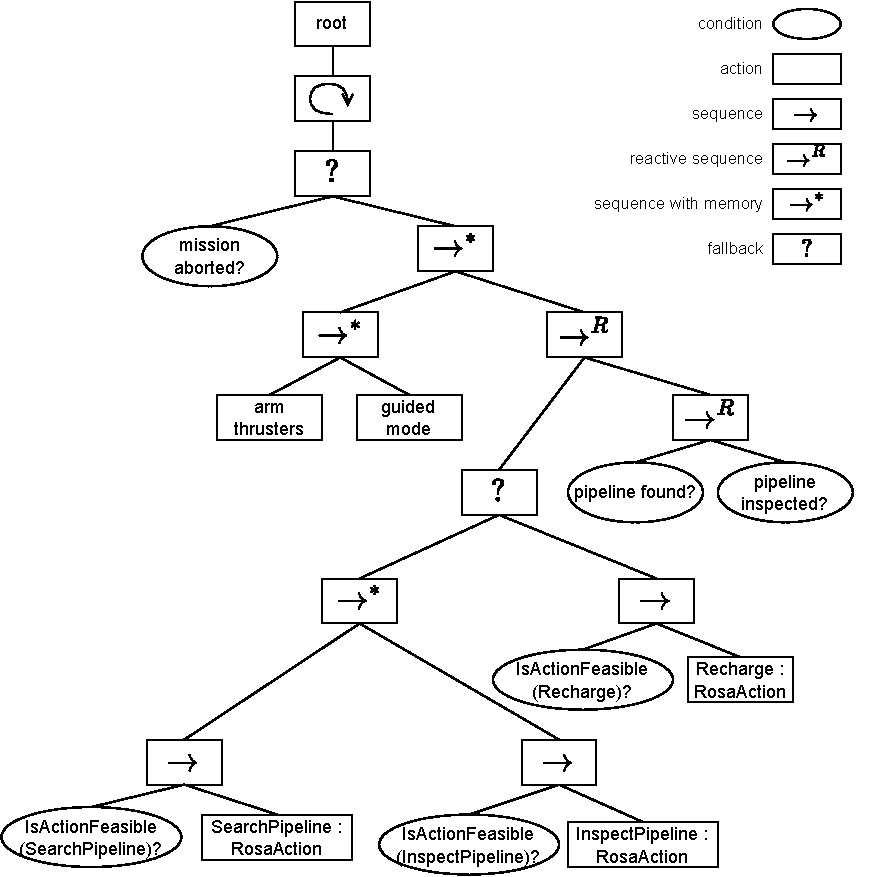
\includegraphics[width=0.7\linewidth]{rosa/figures/suave_extended_rosa_behaviortree_2.pdf}
    \caption{Behavior tree for the extended SUAVE use case}
    \label{fig:bt_extended}
\end{figure}

% \begin{figure}[h]
\begin{lstlisting}[caption=Snippet of SUAVE's use case implementation in TypeDB, label=lst:suave, columns=fullflexible, language=TypeQL]
# Action search pipeline
$a_search_pipeline isa Action, has action-name
    'search_pipeline';

$f_generate_search_path isa Function, has function-name
    'generate_search_path';

# functional-requirement relationship
(action: $a_search_pipeline,
 required-function: $f_generate_search_path,
 required-function: $f_maintain_motion)
 isa functional-requirement;
\end{lstlisting}
% \end{figure}

\begin{figure}[h]
\begin{lstlisting}[caption=Snippet of the PDDL domain formulation for SUAVE containing the search pipeline action definition., label=lst:suave_extended_pddl, columns=fullflexible, language=PDDL]
 (:durative-action search_pipeline
   :parameters (?a - action ?p - pipeline ?r - robot)
   :condition (and
     (over all (robot_started ?r))
     (over all (search_pipeline_action ?a))
     (over all (action_feasible ?a))
   )
   :effect (and
     (at end(pipeline_found ?p))
   )
 )
 ...
\end{lstlisting}
% \vspace{-5ex}
\end{figure}

\subsubsection{Result} During the mission execution, the AUV was able to overcome all uncertainties: adapting to thruster failures ($U_1$) with structural adaptation, to changing water visibility ($U_2$) with parameter adaptation, and to an unexpected drop in the battery level ($U_3$) with TACA, demonstrating the feasibility of using ROSA to enable runtime TACA in ROS 2-based robotic systems.

\subsection{Performance}

\subsubsection{Experimental setup} To evaluate ROSA's performance, the SUAVE exemplar was configured with the same parameters as described in the SUAVE paper~\citep{suave}. In addition, for the extended use case, the battery was set to discharge within 200 seconds, and the \textit{search pipeline} and \textit{inspect pipeline} actions were set to require at least 25\% of battery to be performed.

\subsubsection{Results}
The results obtained are shown in \Cref{tab:results}.
The different managed subsystems had similar performance despite the difference in their reaction time. Furthermore, since the performance with ROSA was better than without a managing subsystem and close to the other
 managing subsystems, it can be considered as additional evidence of the feasibility of applying it at runtime to enable self-adaptation in robotic systems.

\begin{table}[h]
\centering
\caption{Mission results}
\label{tab:results}
\resizebox{\linewidth}{!}{%
\begin{tabular}{p{.13\linewidth}p{.1\linewidth}p{.1\linewidth}p{.1\linewidth}p{.1\linewidth}p{.1\linewidth}p{.1\linewidth}p{.1\linewidth}p{.1\linewidth}}
\hline
\multirow{2}{*}{\begin{tabular}[c]{@{}l@{}}\textbf{Managing} \\ \textbf{system}\end{tabular}} &
  \multirow{2}{*}{\begin{tabular}[c]{@{}l@{}}\textbf{Number} \\ \textbf{of runs}\end{tabular}} &
  \multicolumn{2}{l}{\textbf{Search time (s)}} &
  \multicolumn{2}{l}{\textbf{Distance inspected (s)}} &
  \multicolumn{3}{l}{\textbf{Mean reaction time (s)}} \\ \cline{3-9}
              &              & \textbf{Mean}          & \textbf{Std dev}       & \textbf{Mean}          & \textbf{Std dev}       & \textbf{U1}           & \textbf{U2} & \textbf{U3}        \\ \hline
\multicolumn{9}{l}{\textbf{SUAVE}}                                                                                             \\ \hline
None          & 100          & 174.75       & 36.00         & 33.20         & 13.49         & N/A          & N/A   & N/A         \\
BT            & 100          & 84.09          & 26.41          & 62.70          & 7.78          & 0.08          & 0.10   & N/A         \\
Metacontrol   & 100          & 89.24        & 35.57        & 60.57         & 11.17         & 1.55          & 0.82     & N/A       \\
\textbf{ROSA} & \textbf{100} & \textbf{85.11}  & \textbf{32.48} & \textbf{60.76} & \textbf{10.29} & \textbf{1.24} & \textbf{1.57} & \textbf{N/A} \\ \hline
\multicolumn{9}{l}{\textbf{SUAVE extended}}                                                                                    \\ \hline
BT            & 100          & 94.37          & 34.92          & 20.88          & 3.81          & 0.07           & 0.10   & 1.09          \\
\textbf{ROSA} & \textbf{100} & \textbf{92.75} & \textbf{35.92} & \textbf{18.97} & \textbf{3.38} & \textbf{1.39}  & \textbf{1.67} & \textbf{2.50}   \\ \hline
\end{tabular}%
}
\end{table}

\subsection{Reusability}\label{sec:reusability}
\subsubsection{Autonomous ground vehicle use case~\citep{CAMARASoftwareArchitectureTask2020}}
In this scenario, an AGV has to navigate from an initial to a goal position in a graph-like environment while facing uncertainties such as component failures, corridors with obstacles, and changing light conditions.

The AGV has distinct architectural variants available to solve navigation. It has three localization algorithms (AMCL, MRPT, or aruco) and three sensing components (camera, lidar, or Kinect). However, there are some restrictions on how they can be combined. The AMCL and MRPT algorithms can only be combined with lidar or Kinect, and the aruco algorithm can only be combined with a camera. In low-light conditions, the camera can only be used with a lamp. Furthermore, the robot can move at three different speeds. Each configuration has a different energy cost, safety, and accuracy level. This scenario can be solved with ROSA with the knowledge model depicted in \Cref{fig:camara}\footnote{The accuracy estimation for \emph{fd1} and \emph{fd2} and all energy estimations are omitted from the figure to improve readability}.

\begin{figure}
    \centering
    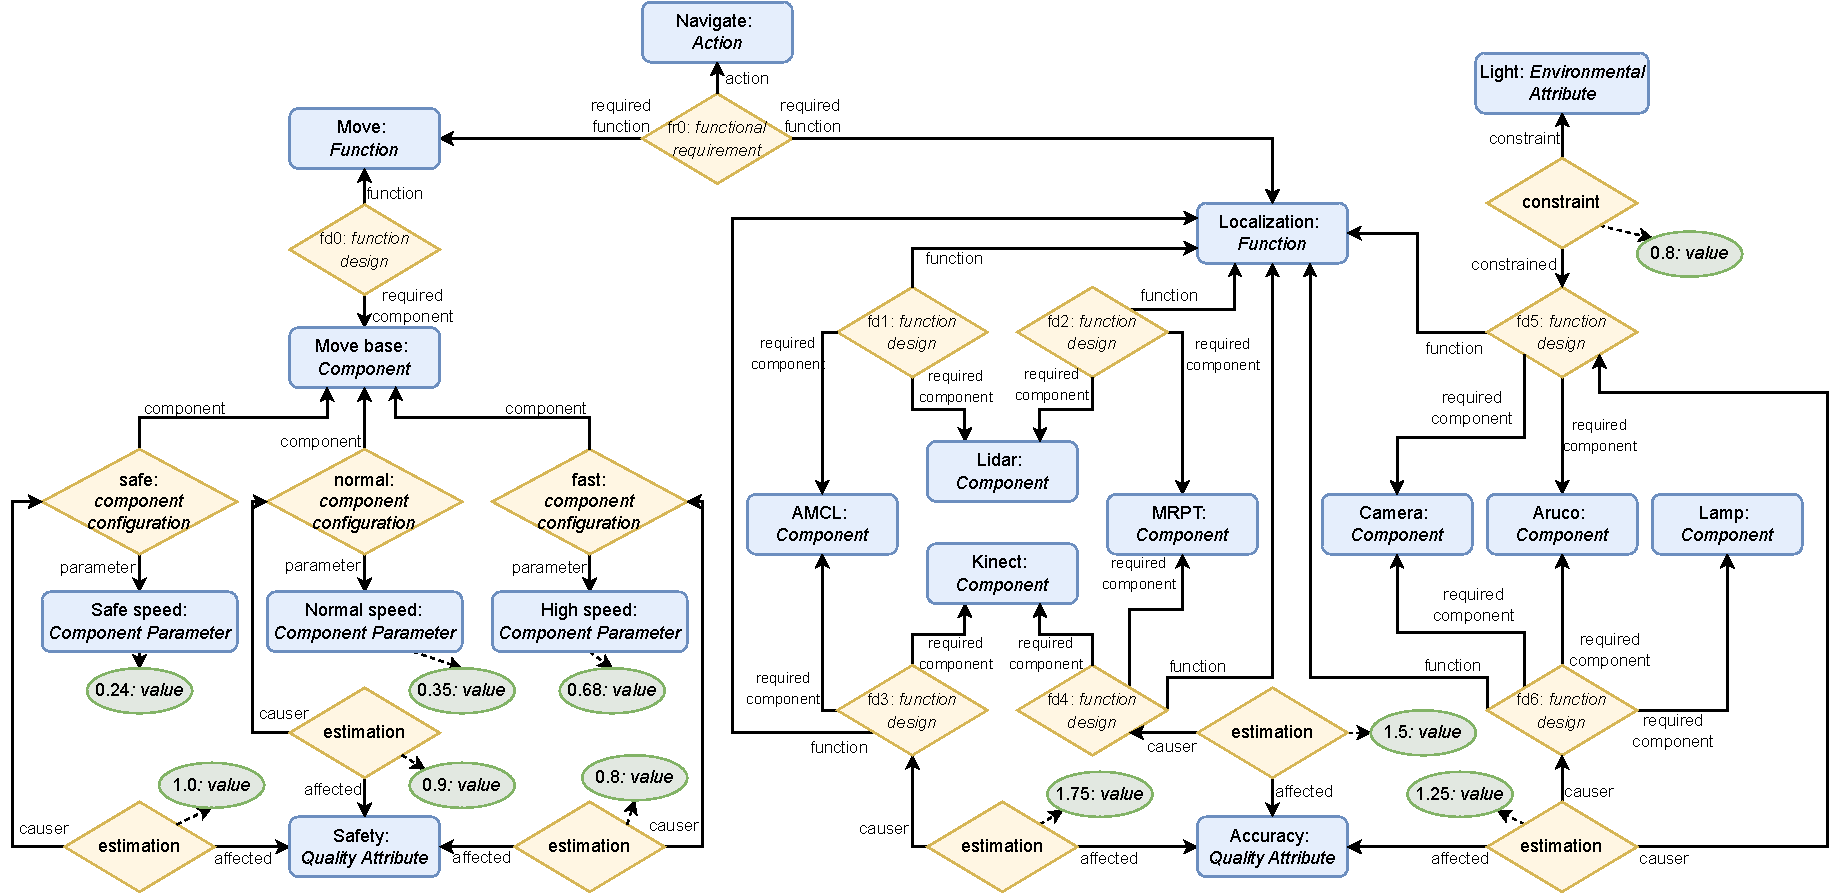
\includegraphics[width=1\linewidth]{rosa/figures/camara_full.pdf}
    \caption{ROSA model for the AGV use case~\citep{CAMARASoftwareArchitectureTask2020}}
    \label{fig:camara}
\end{figure}

When navigating, the robot performs adaptation by selecting which corridors it needs to go through given its feasible configurations, and by selecting a suitable architecture configuration for each corridor it goes through. For example, to go from point $A$ to $B$, the AGV can go directly through a corridor with obstacles $C1$ or through corridors $C4\rightarrow C3\rightarrow C2$ without obstacles. Ideally, the AGV should go through $C1$ as it is the shortest path. Considering that the Kinect and AMCL combination is the only one with enough accuracy to go through a corridor with obstacles, in the case that the Kinect fails, the robot needs to perform TACA by adapting its task plan to go through $C4\rightarrow C3\rightarrow C2$ while simultaneously adapting its architecture, e.g., to use the lidar as its sensing component.

\subsubsection{Unmanned aerial vehicle use case~\citep{braberman2018extended}}\label{sec:morph_example}
In this scenario, a UAV has to search for samples in a predefined area and analyze them. To accomplish this mission, the UAV can perform the actions \emph{(A1) search for samples}, \emph{(A2) pick up and analyze samples}, \emph{(A3) analyze samples on site}, \emph{(A4) return to base and recharge}, and \emph{(A5) land and fold gripper}. The analyze action \emph{A2} performs a better analysis than \emph{A3}, however, it consumes more battery. Furthermore, action \emph{A2} requires a \emph{gripper}, while \emph{A3} requires an \emph{infra-red camera}. When operating, the UAV might run out of battery, and its gripper might fail.

There are three adaptation scenarios in this use case:
\emph{(1)} if the battery level is insufficient to perform \emph{A1}, the UAV must perform \emph{A4}; \emph{(2)} if the battery level is insufficient to perform \emph{A2} but it is still sufficient to perform \emph{A3}, the UAV must perform \emph{A3}; \emph{(3)} if the \emph{gripper} fails while performing \emph{A2}, the UAV must perform \emph{A3}.
Before transitioning from \emph{A2} to \emph{A3}, the UAV must first perform \emph{A5}.

Adaptation scenarios \emph{1} and \emph{2} can be solved with ROSA's knowledge model by capturing the battery level as a \entity{Quality Attribute} and using it as a \relationship{constraint} for actions \emph{A1} and \emph{A2}. Adaptation scenario \emph{3} can be solved by capturing that the \entity{Function} required by \emph{A2} requires a \emph{gripper} component. Furthermore, the task decision layer is responsible for guaranteeing that \emph{A3} is only performed when \emph{A5} is finished.

\subsubsection{Results} This evaluation demonstrates that in addition to SUAVE, the knowledge required for the adaptation logic to solve the AGV and UAV use cases can be captured with ROSA's knowledge model. This indicates that ROSA's knowledge model can be used to capture the knowledge required for TACA in adaptation scenarios similar to the ones presented.
Furthermore, it shows that all entities and relationships contained in the proposed knowledge model had to be used to model the aforementioned adaptation scenarios, supporting their inclusion in the knowledge model.

\subsection{Development effort}

\subsubsection{Experimental Setup}
To measure ROSA's development effort for each use case, we count the number of entities and relationships contained in the models created for the use cases presented. To measure the BT managing system development effort for SUAVE,  we count the number of nodes contained in the BTs created to solve it, and the number of modes and parameters included in the System Modes' configuration file already packaged in SUAVE. In the remainder of this paper, we denote the elements modeled in both approaches as \emph{overhead}.

\subsubsection{Results}  The overhead for both approaches can be seen in \Cref{tab:dev_effort}. Although it is not possible to make a straightforward comparison between the development efforts of both approaches using the observed overheads since the difficulty of modeling an element using the different modeling techniques is subjective, analyzing the reason for the observed overheads provides insights for comparing the development efforts of both approaches.

\begin{table}[h]
\centering
\caption{Development effort of using ROSA and BTs as managing subsystems}
\label{tab:dev_effort}
% \resizebox{\columnwidth}{!}{%
% \begin{tabular}{p{0.2\linewidth}p{0.2\linewidth}p{0.3\linewidth}p{0.08\linewidth}}
\begin{tabularx}{\linewidth}{XXXX}
\hline
\multicolumn{4}{p{\linewidth}}{\textbf{ROSA}}                                                    \\ \hline
\textbf{Use case} & \textbf{Entities}      & \textbf{Relations} & \textbf{Total} \\ \hline
SUAVE             & 18                     & 12                     & 30             \\
SUAVE  extended    & 22                     & 16                     & 38             \\
AGV      & 18                     & 36                     & 54             \\
UAV               & 24                     & 16                     & 40             \\ \hline
\multicolumn{4}{p{\linewidth}}{\textbf{Behavior tree}}                                           \\ \hline
\textbf{Use case} & \textbf{BT} & \textbf{System modes}  & \textbf{Total} \\ \hline
SUAVE             & 27                     & 30                     & 57             \\
SUAVE extended    & 34                     & 38                     & 72             \\ \hline
% \end{tabular}%
\end{tabularx}%
% }
\end{table}

\emph{ROSA:}
In TypeDB, each entity and relationship is inserted in the KB with TypeQL queries such as the ones presented in \Cref{lst:suave}.
Thus, the total number of queries that the roboticist must define to solve an adaptation scenario is equal to the sum of the number of entities and relationships contained in the model, with a clear separation between the task and adaptation logic.

\begin{figure}[h]
    \centering
    % \begin{subfigure}[b]{0.59\textwidth}
        % \centering
        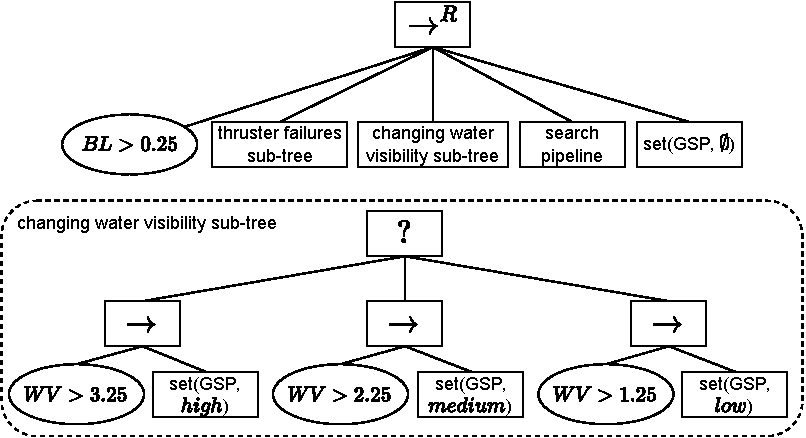
\includegraphics[width=0.7\linewidth]{rosa/figures/behaviortree_search_pipeline_pattern.pdf}
        % \caption{Pattern for SUAVE's search pipeline action adaptations.}
        % \label{fig:bt_pattern_wv}
    % \end{subfigure}
    \hfill
    % \begin{subfigure}[b]{0.39\textwidth}
    %     \centering
    %     \includegraphics[width=\textwidth]{figures/behaviortree_abort_pattern.pdf}
    %     \caption{Pattern for aborting SUAVE's mission.}
    %     \label{fig:bt_pattern_abort}
    % \end{subfigure}
    \caption{Snippet of the BT used to capture SUAVE's task and adaption logic. \emph{WV} and \emph{BL} represent the measured water visibility and battery level, respectively. \emph{GSP}, \emph{MM}, and \emph{FP} represent SUAVE's \emph{generate search path node}, \emph{maintain motion node}, and \emph{follow pipeline node}, respectively. The \emph{set} action changes the system's modes. }
    \label{fig:behaviortree_patterns}
\end{figure}

\emph{BT managing system:}
The BT used to model SUAVE's task logic without adaptation contains 10 nodes, and the BT used for the extended use case contains 16 nodes. These values were deducted from the development effort metric for the BT managing system since they are independent of the adaptation problem.

\Cref{fig:behaviortree_patterns} depicts the pattern used to model SUAVE's \emph{search pipeline} action and its related adaptations\footnote{The full BT can be found in the SUAVE repository.}. As can be seen, there is no separation between the task and adaptation logic, which is the main limitation of using BTs in comparison to using ROSA to model the adaptation logic. The coupling of both logics hinders the reusability of the approach as another system with the same task logic but different adaptation logic, or vice-versa, cannot reuse the existing BTs. In addition, when any changes are made to the task or adaptation problems, it will most likely require changes to parts of the BT that are not necessarily related to the changes introduced. Furthermore, it makes the modeling process more difficult as the roboticist needs to consider both problems simultaneously when modeling the BTs.

\subsection{Development effort scalability}
\subsubsection{Experimental setup}
To evaluate how ROSA's development effort scales for more complex use cases, we analyze how the development effort of a base scenario grows with the addition of new actions and adaptations.
The growth for adding actions and adaptations depends on the specific application.
Thus, we make the following assumptions to generalize and simplify the analysis of adding adaptation.

\begin{assumption}\label{as:1}
Every action requires one function that has only one configuration available consisting of a single component with no parameters.
\end{assumption}

\begin{assumption}\label{as:2}
Every \entity{Component} is a \entity{ROSNode} containing one \attribute{package} and one \attribute{executable} attribute; every \entity{ROSNode} has one \relationship{component configuration} with one \entity{Component Parameter}; every \relationship{function design} and \relationship{component configuration} must be related to a \relationship{constraint} and contain a \attribute{priority} attribute; and a single \entity{Quality Attribute} is defined for the whole system.
\end{assumption}

\begin{figure}
    \centering
    \begin{minipage}[b]{0.3\textwidth}
        \centering
        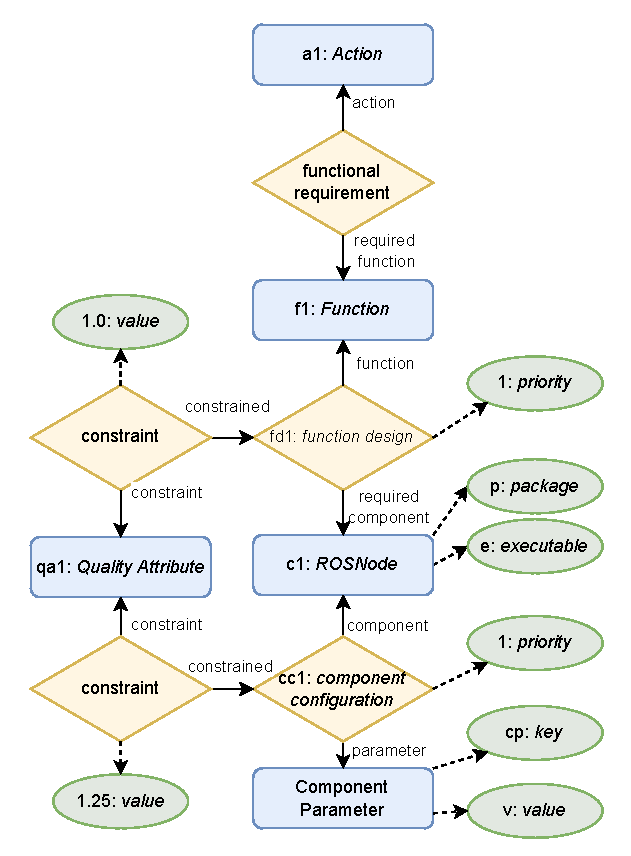
\includegraphics[width=\textwidth]{rosa/figures/overhead_base_model.pdf}
        \caption{Base model}
        \label{fig:base_model}
    \end{minipage}
    \hfill
    \begin{minipage}[b]{0.3\textwidth}
        \centering
        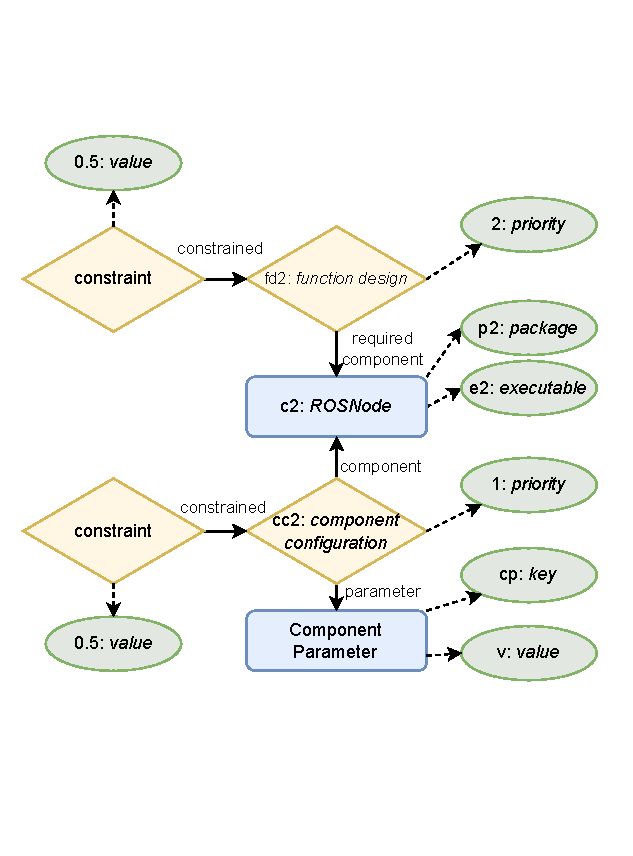
\includegraphics[width=\textwidth]{rosa/figures/overhead_structural.pdf}
        \caption{Structural adaptation}
        \label{fig:overhead_structural}
    \end{minipage}
    \hfill
    \begin{minipage}[b]{0.3\textwidth}
        \centering
        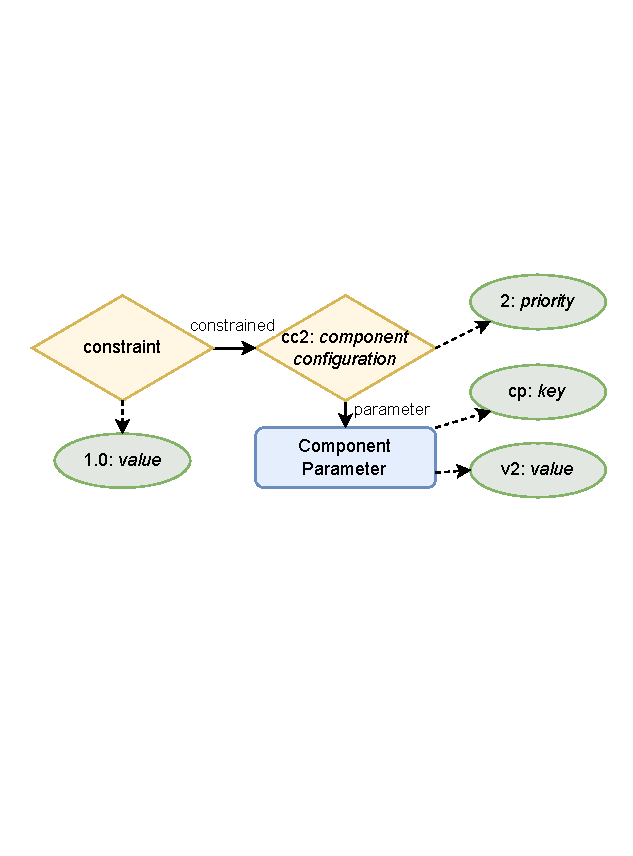
\includegraphics[width=\textwidth]{rosa/figures/overhead_parameter.pdf}
        \caption{Parameter adaptation}
        \label{fig:overhead_parameter}
    \end{minipage}

    \caption{Minimum knowledge required to model adaptation given Assumptions \ref{as:1} and \ref{as:2}. The name attribute is depicted as \textit{name: Entity} or \textit{name: Relationship} inside each diamond and rectangle shape, respectively.}
    \label{fig:overhead}
\end{figure}

\subsubsection{Results}
Consider a base scenario where the robot has only one action and complies with Assumptions~\ref{as:1} and~\ref{as:2}. The ROSA model to solve it contains $10$ elements and is depicted in \Cref{fig:base_model}.

To add structural adaptation to the base scenario (given Assumption~\mbox{\ref{as:2}}), it is necessary to add the elements depicted in \Cref{fig:overhead_structural} to the model.
This results in a minimum overhead of $6$ elements for each structural adaptation. To add parameter adaptation to the base scenario (given Assumption~\mbox{\ref{as:2}}), it is necessary to add the elements depicted in \Cref{fig:overhead_parameter} to the model.
This results in a minimum overhead of $3$ elements for each parameter adaptation.

In conclusion, given Assumptions~\ref{as:1} and~\ref{as:2}, the total overhead per action can be defined as $10 + 6*n_{sa} + 3*n_{pa}$, where $n_{sa}$ and $n_{pa}$ represent the number of structural and parameter adaptations for the action, respectively.
This indicates that the ROSA model grows linearly with the number of actions and adaptations, which is made possible by the clear separation of the task and adaptation logic.


\section{Conclusions and future work}\label{sec:rosa:conclusion}
This work proposed ROSA, a knowledge-based solution for task-and-architecture co-adaptation in robotic systems that promotes reusability, extensibility, and composability. Reusability was achieved by proposing a knowledge model that can capture the knowledge required for TACA and using it at runtime to reason about adaptation. Extensibility and composability were achieved with an architectural design that allows ROSA's components to be stateless and self-contained. The feasibility of using ROSA in robotic systems at runtime was demonstrated by applying it in simulation to the SUAVE exemplar. ROSA's reusability was demonstrated by using it to model different self-adaptive robotic systems and showing that it can capture all relevant knowledge for adaptation necessary for these use cases.  Furthermore, ROSA's development effort and its scalability were demonstrated for the use cases presented in this paper and for a hypothetical scenario.

\chapter{Plan your Self-Adaptation! -- Ontology-Mediated Task and Architecture Co-adaptation Planning for Robots}
\label{pddl}

\begin{abstract}
  Autonomous robots may need to adapt both their task plans and architectural configurations as operating conditions change. These decisions are interdependent: architectural configurations determine which actions a robot can perform, while task plans determine which capabilities are required. This paper presents \acronym, an ontology-mediated approach to task and architecture co-adaptation that considers these dependencies during mission planning. \acronym uses an ontology expressed in the Web Ontology Language to represent architectural alternatives and their associated functional and quality requirements, while the Planning Domain Definition Language defines task actions and mission goals. By automatically translating and integrating these models, \acronym enables joint planning of task and reconfiguration actions. The approach uses satisficing planning and replans when changes during execution invalidate the current plan. \acronym is evaluated in two robotic scenarios involving underwater inspection and ground navigation. The results support the feasibility of runtime co-adaptation and show lower planning time and memory consumption compared with optimal-policy generation in the evaluated navigation scenario, while producing plans of similar quality. % chktex 12 -- sentence starts with a macro
\end{abstract}

\blfootnote{This chapter is a verbatim copy of the paper~\cite{silva2025planyour}.
\begin{itemize}
    \item \textbf{Gustavo Rezende Silva}, Tobias John, Francisco Martín, Einar Broch Johnsen, and Carlos Hern{\'a}ndez Corbato. ``Plan your Self-Adaptation! -- Ontology-Mediated Task and Architecture Co-adaptation Planning for Robots.'' Submitted to ACM Transactions on Autonomous and Adaptive Systems.
\end{itemize}
}

\newpage

% The files under pddl/sections/, pddl/figures/, pddl/tables/,
% pddl/navigation_experiment/ and pddl/config/ are generated from the paper
% sources by pddl/sync_from_paper.py. Do not edit them here; edit the paper and
% re-run the script.

\section{Abstract}

  Autonomous robots may need to adapt both their task plans and architectural configurations as operating conditions change. These decisions are interdependent: architectural configurations determine which actions a robot can perform, while task plans determine which capabilities are required. This paper presents \acronym, an ontology-mediated approach to task and architecture co-adaptation that considers these dependencies during mission planning. \acronym uses an ontology expressed in the Web Ontology Language to represent architectural alternatives and their associated functional and quality requirements, while the Planning Domain Definition Language defines task actions and mission goals. By automatically translating and integrating these models, \acronym enables joint planning of task and reconfiguration actions. The approach uses satisficing planning and replans when changes during execution invalidate the current plan. \acronym is evaluated in two robotic scenarios involving underwater inspection and ground navigation. The results support the feasibility of runtime co-adaptation and show lower planning time and memory consumption compared with optimal-policy generation in the evaluated navigation scenario, while producing plans of similar quality. % chktex 12 -- sentence starts with a macro

\section{Introduction}

Autonomous robots are required to operate reliably in increasingly complex environments and to perform a larger number of tasks with distinct functional and quality requirements, potentially requiring different architectural configurations to satisfy them. A key challenge in designing such systems is ensuring that the robot continues to meet its requirements throughout mission execution, particularly under uncertainty, such as sensor failures or environmental disturbances~\cite{Correll-2017, Krotkov-2018}. For example, an underwater robot might require different sensor configurations depending on the water visibility, or it might need to navigate through different paths depending on water currents. Addressing these challenges requires coordinating task execution and architectural adaptation while accounting for their interdependencies.

Task and architecture co-adaptation (TACA)~\cite{CAMARASoftwareArchitectureTask2020} addresses the interdependencies between task execution and architectural adaptation. Reactive TACA approaches such as ROSA~\cite{rosa} select a configuration for each action only when that action begins executing, without accounting for how the choice constrains the rest of the mission. However, selecting a suitable configuration for the current action alone does not establish whether subsequent actions can be performed under the conditions anticipated along the mission. Considering these dependencies during mission planning allows configuration requirements to influence the task plan before execution begins, so that each configuration choice is made with its downstream task consequences in view. To the best of our knowledge, the approach by Cámara et al.~\cite{CAMARASoftwareArchitectureTask2020} is the only approach that jointly plans task actions and reconfiguration actions and produces a complete plan ahead of execution. Their approach, however, requires substantial planning time and memory and relies on domain models expressed across multiple specification languages with manually developed integration code, increasing modeling effort and the potential for errors. Furthermore, their approach requires modeling probabilities to enable optimal planning, although these probabilities can be difficult to estimate accurately.

To address these limitations, this paper proposes \acronym, an ontology-mediated approach that formulates task and architecture co-adaptation as a single planning problem by automatically integrating task and architectural knowledge. \acronym uses a Web Ontology Language (OWL) ontology~\cite{aguado2024survey} to represent the functional requirements of robot actions, the architectural alternatives that realize those requirements, and the quality attributes and requirements used to assess the applicability and utility of each alternative. The Planning Domain Definition Language (PDDL)~\cite{karpas2020automated} describes task actions, the current system state, and mission goals. % chktex 12
Architectural knowledge is automatically translated into PDDL and integrated with the task model, allowing task actions and architectural reconfiguration actions to be considered within the same search space. This integration preserves a separation between task modeling and architectural knowledge modeling. The resulting problem can be solved by standard PDDL planners. To support timely runtime adaptation, \acronym favors satisficing planning over guaranteed mission-level optimality. Rather than explicitly modeling uncertainty and its probabilities, it plans from the currently observed state and handles changes during execution through replanning when monitored conditions invalidate the current plan. By relying on two established modeling languages and automating their integration, \acronym aims to reduce modeling effort.

\begin{figure}[tbp]
	\centering
        \resizebox{\textwidth}{!}{
            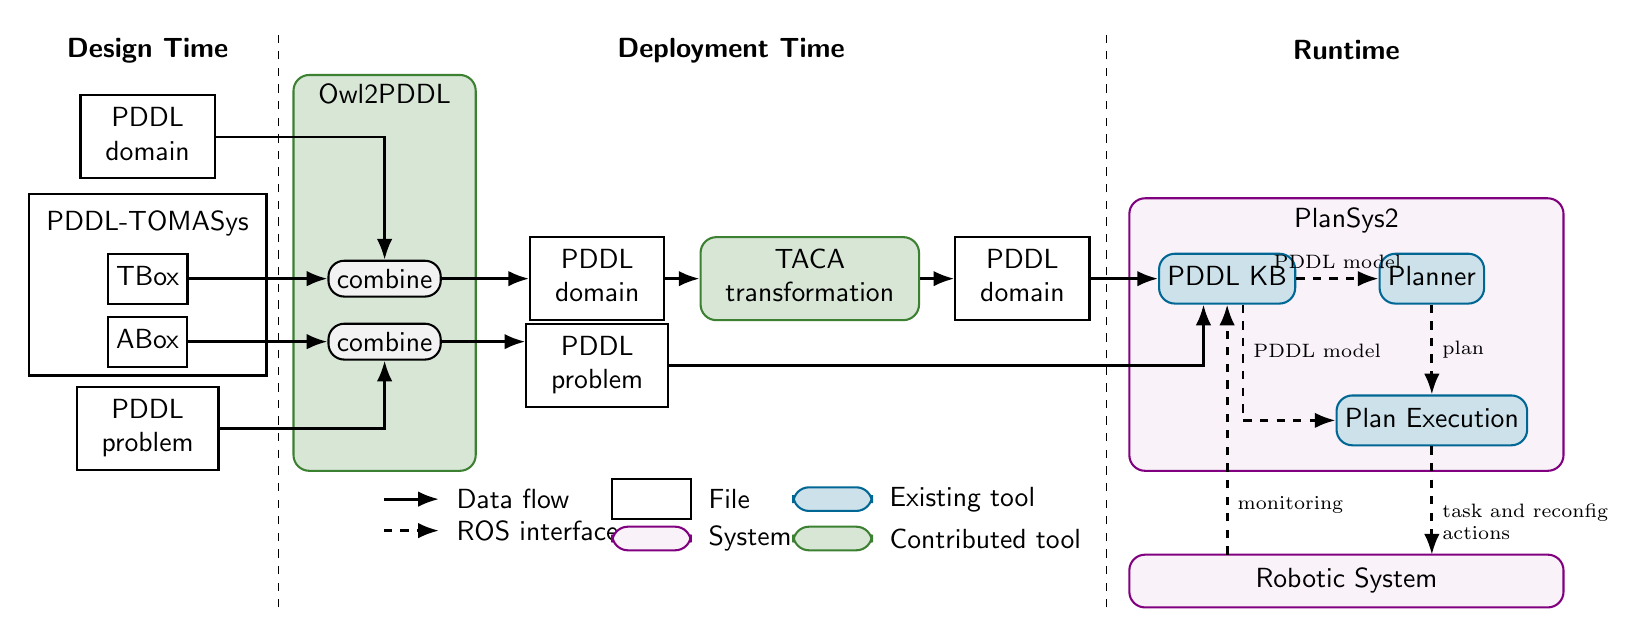
\begin{tikzpicture}[font=\sffamily]

    \coordinate (origin) at (0,0);
    \draw (origin) node (design_time) {\textbf{Design Time}};

    \draw ($(design_time) + (0, -1.1)$) node[artifact] (domain)
    {\begin{tabular}{c}
        PDDL\\
        domain
    \end{tabular}};

    \draw ($(domain) + (0.0, -1.1)$) node (ontology) {PDDL-TOMASys};

    \draw ($(ontology) + (0.0, -0.7)$) node[artifact] (tbox) {TBox\strut};
    \draw ($(tbox) + (0.0, -0.8)$) node[artifact] (abox) {ABox\strut};

    % outline of ontology
    \coordinate (bottom_point_ontology) at (abox.south -| ontology.east);
    \draw[artifact_transparent] ($(ontology.north west) + (-0.1, 0.1)$) rectangle ($(bottom_point_ontology) + (0.1, -0.1)$);

    \draw ($(abox) + (0, -1.1)$) node[artifact] (problem)
    {\begin{tabular}{c}
        PDDL\\
        problem
    \end{tabular}};

     % OWL2PDDL
    \coordinate (domain1_north_ontology_east) at (domain.north -| ontology.east);
    \draw ($(domain1_north_ontology_east) + (1.6, 0)$) node[minimum width=2.3cm] (owlTool) {\owltopddl};
    \begin{pgfonlayer}{background}
        % \coordinate (help2) at ($(combine2.south) + (0, -0.2)$);
        \coordinate (bottom_owl2pddl) at (problem.south -| owlTool.east);
        \draw[tool] (owlTool.north west) rectangle ($(bottom_owl2pddl)$);
    \end{pgfonlayer}

    \draw (owlTool |- tbox) node[process] (combine_domain) {combine} ;
    \draw (owlTool |- abox) node[process] (combine_problem) {combine}  ;

    % arrows
    \draw[arrow] (domain) -| (combine_domain);
    \draw[arrow] (problem) -| (combine_problem);
    \draw[arrow] (tbox) -- (combine_domain);
    \draw[arrow] (abox) -- (combine_problem);

    \draw ($(combine_domain) + (2.7, 0.0)$) node[artifact] (domain2)
    {\begin{tabular}{c}
        PDDL\\
        domain
    \end{tabular}};
    \draw ($(combine_problem) + (2.7, -0.3)$) node[artifact] (problem2)
    {\begin{tabular}{c}
        PDDL\\
        problem
    \end{tabular}};
    \draw[arrow] (combine_domain) -- (domain2);
    \draw[arrow] (combine_problem) -- (combine_problem -| problem2.west);

    \draw ($(domain2) + (2.7, 0)$) node[tool] (taca)
    {\begin{tabular}{c}
        TACA\\
        transformation
    \end{tabular}};

    \draw[arrow] (domain2) -- (taca);

    \draw ($(origin.north -| taca) + (-1,0)$) node (deployment_time) {\textbf{Deployment Time}};

    \draw ($(taca) + (2.7, 0.0)$) node[artifact] (domain3)
    {\begin{tabular}{c}
        PDDL\\
        domain
    \end{tabular}};
    \draw[arrow] (taca) -- (domain3);

     % PlanSys2
    \coordinate (domain1_north_domain3_east) at (domain3.north -| domain3.east);
    \draw ($(domain1_north_domain3_east) + (3.25, 0.2)$) node[minimum width=5.5cm] (plansys) {PlanSys2};
    \begin{pgfonlayer}{background}
        % \coordinate (help2) at ($(combine2.south) + (0, -0.2)$);
        \coordinate (bottom_plansys) at (problem.south -| plansys.east);
        \draw[system] (plansys.north west) rectangle ($(bottom_plansys)$);
    \end{pgfonlayer}

    \draw ($(domain3) + (2.6, 0.0)$) node[tool_3rd_party] (pddl_kb){PDDL KB\strut};
    \draw[arrow] (domain3) -- (pddl_kb);
    \coordinate (problem2_pddl_kb_in) at (pddl_kb.south -| pddl_kb);
    \draw[arrow] (problem2) -| ($(pddl_kb.south -| pddl_kb) + (-0.3, 0)$);

    \draw ($(pddl_kb) + (2.6, 0.0)$) node[tool_3rd_party] (planner){Planner\strut};
    \draw[arrow_dashed] (pddl_kb) -- (planner)
        node[midway, above, font=\scriptsize] {PDDL model};

    \draw ($(planner) + (0.0, -1.8)$) node[tool_3rd_party] (plan_exec){Plan Execution\strut};
    \draw[arrow_dashed] (planner) -- (plan_exec)
        node[midway, right, font=\scriptsize] {plan};
    \coordinate (pddlkb_plan_exec_arrow) at (pddl_kb.south -| pddl_kb);
    \draw[arrow_dashed] ($(pddlkb_plan_exec_arrow) + (0.2, 0.0)$) |- (plan_exec)
        node[pos=0.2, right, font=\scriptsize] {PDDL model};

    % \coordinate (robot_start) at (problem.south -| plansys.west);
    \draw ($(problem.south -| plansys) + (0.0, -1.4)$) node[minimum width=5.5cm] (robot){Robotic System\strut};
    \begin{pgfonlayer}{background}
        % \coordinate (help2) at ($(combine2.south) + (0, -0.2)$);
        \coordinate (bottom_plansys) at (problem.south -| plansys.east);
        \draw[system] (robot.north west) rectangle ($(robot.south east) + (0.0, -0.0)$);
    \end{pgfonlayer}

    \draw[arrow_dashed] (plan_exec) -- (robot.north -| plan_exec)
        node[pos=0.7, right, font=\scriptsize, align=left] {task and reconfig\\actions};
    \draw[arrow_dashed] (robot.north -| pddl_kb) -- (pddl_kb)
        node[pos=0.2, right, font=\scriptsize] {monitoring};

    \draw[dashed] ($(robot.south -| ontology.east) + (0.25, 0)$) -- ($(design_time.north -| ontology.east) + (0.25, 0)$);
    \draw[dashed] ($(robot.south -| domain3.east) + (0.2, 0)$) -- ($(design_time.north -| domain3.east) + (0.2, 0)$);

    \draw ($(origin.north -| plansys)$) node (run_time) {\textbf{Runtime}};

    \begin{scope}[shift={(3.0,-5.7)}]
        \draw[arrow] (0,0) -- (0.7,0);
        \node[right] at (0.8,0) {Data flow};
        \draw[arrow_dashed] (0,-0.4) -- (0.7,-0.4);
        \node[right] at (0.8,-0.4) {ROS interface};
        \node[artifact] at (3.4, 0) {};
        \node[right] at (4,0) {File};
        \node[system] at (3.4, -0.5) {};
        \node[right] at (4,-0.5) {System};
        \node[tool_3rd_party] at (5.7, 0.0) {};
        \node[right] at (6.3,0.0) {Existing tool};
        \node[tool] at (5.7, -0.5) {};
        \node[right] at (6.3,-0.5) {Contributed tool};
    \end{scope}
\end{tikzpicture}


% \begin{tikzpicture}[font=\sffamily]

%     \coordinate (origin) at (0,0);
%     \draw (origin) node[artifact] (domain) {PDDL domain\strut};

%     \draw ($(domain) + (0, -1)$) node[artifact] (problem) {PDDL problem\strut};

%     \draw ($(problem) + (2.5, -1.2)$) node[artifact] (tbox) {TBox\strut};
%     \draw ($(tbox) + (1.2, 0)$) node[artifact] (abox) {ABox\strut};

%     \draw ($(tbox) + (0.6, -0.6)$) node (ontology) {PDDL-TOMASys};
%     % outline of ontology
%     \coordinate (help1) at (ontology.south -| tbox.west);
%     \draw[artifact] ($(help1) + (-0.1, -0.1)$) rectangle ($(abox.north east) + (0.1, 0.1)$);

%     \draw (tbox |- domain) node[process] (combine1) {combine} ;
%     \draw (abox |- problem) node[process] (combine2) {combine}  ;

%     \draw ($(domain) + (6, 0)$) node[artifact] (domain2) {PDDL domain\strut};
%     \draw (domain2 |- problem) node[artifact] (problem2) {PDDL problem\strut};

%     \draw ($(domain2) + (3, 0)$) node[tool] (taca)
%     {\begin{tabular}{c}
%         TACA\\
%         transformation
%     \end{tabular}};

%     \draw ($(problem2) + (2.8, -0.2)$) node[process] (update) {update values\strut};
%     \draw ($(update) + (0.6, -1)$) node[process, rounded corners=0.5cm] (monitor) {\begin{tabular}{c}
%             plan execution\\
%             and monitoring
%     \end{tabular}};

%     \draw ($(taca) + (3.5, 0)$) node[artifact] (domain3) {PDDL domain\strut};
%     \draw (domain3 |- problem2) node[artifact] (problem3) {PDDL problem\strut};

%     \draw ($(domain3) + (2.5, -0.5)$) node[tool, minimum height=1.5cm] (planner) {\begin{tabular}{c}
%             PDDL\\
%             planner
%         \end{tabular}};

%     \draw (monitor -| planner) node[artifact] (plan) {plan\strut};

%     % OWL2PDDL
%     \draw ($(ontology) + (0, 3.6)$) node[minimum width=3cm] (owlTool) {OWL2PDDL};
%     \begin{pgfonlayer}{background}
%         \coordinate (help2) at ($(combine2.south) + (0, -0.2)$);
%         \draw[tool] (owlTool.north west) rectangle (owlTool.east |- help2);
%     \end{pgfonlayer}

%     %PlanSys
%     \draw ($(update) + (0.3, 0.5)$) node[minimum width=3.4cm] (plansys) {PlanSys2};
%     \begin{pgfonlayer}{background}
%         \coordinate (help3) at ($(monitor.south) + (0, -0.2)$);
%         \draw[tool] (plansys.north west) rectangle (plansys.east |- help3);
%     \end{pgfonlayer}

%     % runtime stuff
%     \draw ($(plansys) + (-1, -3.2)$) node[runtime] (runtime) {\begin{tabular}{c}
%             runtime\\
%             values
%         \end{tabular}};

%     \draw ($(plansys) + (1, -3.2)$) node[runtime] (actions) {\begin{tabular}{c}
%             actions of\\
%             system
%     \end{tabular}};

%     % arrows
%     \draw[arrow] (domain) -- (combine1);
%     \draw[arrow] (problem) -- (combine2);
%     \draw[arrow] (tbox) -- (combine1);
%     \draw[arrow] (abox) -- (combine2);

%     \draw[arrow] (combine1) -- (domain2);
%     \draw[arrow] (combine2) -- (problem2);

%     \draw[arrow] (domain2) -- (taca);
%     \draw[arrow] (problem2.east |- update) -- (update);

%     \draw[arrow] (taca) -- (domain3);
%     \draw[arrow] (update) -- (problem3.west |- update);

%     \draw[arrow] (domain3) -- (domain3 -| planner.west);
%     \draw[arrow] (problem3) -- (problem3 -| planner.west);

%     \draw[arrow] (planner) -- (plan);
%     \draw[arrow] (plan) -- (monitor);

%     \coordinate (help4) at ($(runtime.north) + (-0.2, 0)$);
%     \draw[arrow] (help4) -- (update.south -| help4);

%     \coordinate (help5) at ($(runtime.north) + (0.5, 0)$);
%     \draw[arrow] (help5) -- (monitor.south -| help5);

%     \draw[arrow] (monitor.south -| actions) -- (actions);



% \end{tikzpicture}
        }
		\caption{\acronym framework, organized into design time, deployment time, and runtime, separated by dashed vertical lines. Some \plansys nodes are omitted for clarity, and the Planner and Plan Execution components shown were extended as part of this work.}%
	\label{planta:fig:architecture}
\Description{Left-to-right diagram of the \acronym workflow. At design time, a PDDL domain and
problem and a \pddltomasys ontology are specified. At deployment time, \owltopddl
combines the ontology TBox with the domain and the ABox with the problem. The TACA
transformation then modifies the domain. At runtime, the resulting domain and problem
populate the \plansys PDDL knowledge base, which supplies the planner and plan execution
component. The planner sends a plan to plan execution, which sends task and
reconfiguration actions to the robotic system. Monitoring feeds observations from the
robot back to the knowledge base. Solid arrows denote data flow and dashed arrows denote
ROS interfaces.}
\end{figure}

\Cref{planta:fig:architecture} depicts the \acronym framework across design time, deployment time, and runtime. At design time, the system architecture is modeled using the \pddltomasys ontology, and the task problem is modeled in PDDL\@. At deployment time, \owltopddl translates the ontology into PDDL, combines it with the planning problem, and incorporates their mutual dependencies, i.e., TACA concerns. At runtime, the planning system, based on \plansys, jointly plans and executes task and reconfiguration actions. \pddltomasys builds upon the Teleological and Ontological Metamodel for Autonomous Systems~(\tomasys)~\cite{aguado2021functional,corbato2013model} and draws inspiration from the ROSA model~\cite{rosa}. % chktex 12

\acronym is evaluated with respect to feasibility, performance efficiency, and scalability on two use cases: an autonomous underwater vehicle~(AUV) scenario from the SUAVE exemplar~\cite{suave}, and an autonomous ground vehicle~(AGV) scenario adapted from~\cite{CAMARASoftwareArchitectureTask2020}. These dimensions are formulated as research questions RQ1--RQ3 in \Cref{planta:sec:evaluation}.
Feasibility (RQ1) is addressed by implementing \acronym and integrating it with \plansys, an existing planning system for robotics. This required extending \plansys with derived predicates and existential preconditions~\cite{edelkamp2004pddl2}, PDDL constructs that the models generated by \owltopddl rely on.
The results of running \acronym on the ROS~2-based SUAVE exemplar support the feasibility of applying it to robotic systems.
Performance efficiency (RQ2) is assessed on the AGV use case, where \acronym is, at the median, $3.00$ times faster than the approach by Cámara et al.~\cite{CAMARASoftwareArchitectureTask2020} and its peak memory usage is $6.84$ times smaller, while both approaches produce plans with near-identical path length and estimated remaining battery at the end of the mission.
In the AGV use case, scalability (RQ3) is assessed by varying the map size, the number of architectural configurations, the number of quality requirements, and the number of mission-level PDDL action schemas, independently and in combination. The results show that satisficing planning remains tractable in scenarios where optimal planning becomes impractical, supporting the use of \acronym in robotic applications that require online task-level replanning.

The main contributions of this paper are:
\begin{enumerate}
    \item an ontology-mediated planning approach for mission-wide task and architecture co-adaptation that combines task and reconfiguration actions in a single PDDL formulation and supports satisficing planning with runtime replanning.
    \item an open-source implementation of the proposed approach, designed for integration with ROS~2-based robotic systems, including an extension of the \plansys framework to support derived predicates and existential preconditions in PDDL\@.
    \item a systematic evaluation of the proposed approach, including a comparison with the state-of-the-art approach by Cámara et al.~\cite{CAMARASoftwareArchitectureTask2020} and a scalability analysis that demonstrates the feasibility of satisficing planning in regimes where optimal planning becomes impractical.
\end{enumerate}


%%% Local Variables:
%%% mode: latex
%%% TeX-master: "main"
%%% End:

\section{Running Example}\label{planta:sec:running_example}

Throughout this paper, the SUAVE exemplar~\cite{suave} is used as a running example to illustrate the concepts introduced by \acronym. In SUAVE, an Autonomous Underwater Vehicle (AUV) carries out an underwater pipeline inspection mission. The mission is structured as a sequence of task actions: \emph{A1}~search for the pipeline, and \emph{A2}~follow and inspect the pipeline. The SUAVE scenario is extended in ROSA~\cite{rosa} with a third action, \emph{A3}~recharge battery, so that the scenario requires task and architecture co-adaptation.

During mission execution, the AUV is subject to three sources of uncertainty. \Uone corresponds to thruster failures: if a thruster fails during \emph{A1} or \emph{A2}, the system requires reconfiguring the architecture to recover the affected thruster. \Utwo corresponds to the variation in water visibility: reduced visibility during \emph{A1} causes the system to select a lower-altitude search configuration. Both \Uone and \Utwo require architecture-level adaptation only, leaving the task plan unchanged. \Uthree corresponds to a critical drop in battery level: if battery level reaches a critical threshold during \emph{A1} or \emph{A2}, the system must interrupt the current action and execute \emph{A3}, which requires a dedicated architectural configuration. Hereafter, the scenario with \Uone and \Utwo is called the original use case, and the scenario with all three uncertainties the extended use case. % chktex 12 -- sentence starts with a macro

In this work, each task action in the mission is encoded as a PDDL action in the planning domain. For example, the \texttt{search\_pipeline} action~(Listing~
\ref{planta:lst:search_pipeline}) encodes \emph{A1}. Throughout the paper, this action is used to illustrate how \acronym transforms a regular action into a managed action that integrates functional and quality requirements derived from the \pddltomasys ontology~(Listing~\ref{planta:lst:search_pipeline_managed}), as described in Section~\ref{planta:sec:plan_transformation_taca}.

\section{Related Works}\label{planta:sec:related}

\subsection{Self-Adaptive Robotic Systems}\label{planta:sec:related_sas}

The mapping study on ``robotics software architecture-based self-adaptive systems''~(RSASSs) by Alberts et al.~\cite{ALBERTS2025112258} identified 37 primary studies published since 2011. Among these, only four works~\cite{park2012task, runtime_variability_lotz, rra_nico, CAMARASoftwareArchitectureTask2020} explicitly address, to varying extents, the dependencies between task execution and architectural adaptation. Additionally, the two studies~\cite{braberman2018extended, temoto} also explore this relationship,  and the ROSA framework proposes a systematic solution to TACA~\cite{rosa}. However, only the approaches~\cite{braberman2018extended, CAMARASoftwareArchitectureTask2020,rosa} fully address TACA\@.
With respect to knowledge-based methods, Alberts et al.\ identified six works~\cite{park2012task, stefan_adaptive_runtime_models, graph_based_nico, p20_stefan_ice, p26_darko_jasper, suave} that utilize knowledge representation techniques to encode the information required for adaptation. From these, the works~\cite{p26_darko_jasper, suave} focus on demonstrating the use of Metacontrol~\cite{hernandez2018self, bozhinoski2022mros} in specific robotic applications rather than proposing complete solutions for RSASSs.
Concerning planning, using PDDL-based planners for RSASSs is still mostly unexplored. Alberts et al.\ identified only the approach \enquote{Model Based Diagnosis (MBD)}~\cite{zaman2013integrated, zaman2019fault}, which employs PDDL-based planning to generate architectural adaptation plans, without explicitly targeting TACA\@.

Cámara et al.~\cite{CAMARASoftwareArchitectureTask2020} proposed a solution to TACA that generates an optimal policy for task execution and architectural configuration. Their method is decomposed into four steps: (i) generate all legal architectural configurations based on the robot’s architecture model, (ii) generate all possible reconfiguration plans between configurations, (iii) generate the \emph{N} best task plans to accomplish the robot's mission goal, (iv) compute an optimal policy for task execution and configuration, given the reconfiguration and task plans. Their experiments show that the generation time is impractical: Generating an optimal task and configuration policy for an AGV operating in a graph-like environment with 58 nodes and with six architectural configurations available takes, on average, $15.1$ seconds.

Silva et al.~\cite{rosa} proposed ROSA as a solution to TACA, focusing on providing a reference framework for robot self-adaptation that promotes reusability, composability, and extensibility. A limitation of ROSA is that it only supports reactive adaptation of the robot's configuration. ROSA determines the robot's configuration for each action only when it starts executing, and it does not produce a complete configuration plan ahead of time.

To address the limitations of these approaches, this work proposes an ontology-mediated planning approach that enables the timely computation of a satisficing task and configuration plan without relying on probabilistic models of real-world uncertainties.
% In conclusion, the method proposed by Cámara et al.~\cite{CAMARASoftwareArchitectureTask2020} is, to the best of our knowledge, the only approach that plans task actions and reconfiguration actions jointly and produces a complete plan ahead of execution. However, it presents practical limitations: it relies on prior knowledge of the probabilities associated with real-world uncertainties, which are often difficult to obtain in practice. Moreover, due to its focus on computing optimal solutions, the method is not fast enough for reactive use in many real-world robotics scenarios, where timely decision-making is critical. To address these limitations, this work proposes an ontology-mediated planning approach that enables the timely computation of a satisficing task and configuration plan without relying on probabilistic models of real-world uncertainties.


\subsection{Combining Ontologies and Planning}\label{planta:sec:related_ontology_planning}

\paragraph{Knowledge and Action Bases.}
Several works have explored combining ontologies with planning problems. The approach proposed in this work is most closely related to the work on \emph{Knowledge and Action Bases (KABs)}~\cite{DBLP:journals/jair/HaririCMGMF13}, where an ontology is used to provide additional insights about a planning state by using queries to the ontology in the planning domain. The actions in the planning domain describe changes to the ontology over time.

There are different approaches to generate a plan for KABs, namely (i) rewriting ontology queries to complex preconditions~\cite{DBLP:conf/ijcai/CalvaneseMPS16}, (ii) rewriting ontology axioms to derived predicates~\cite{DBLP:conf/aaai/Borgwardt0KKNS22}, and (iii) enriching the planning domain with grounded answers to the ontology queries~\cite{DBLP:conf/ecai/JohnK24}. All the approaches have in common that they perform planning as a two-step process: First, the ontology is analyzed and a new planning domain is created that encodes the axioms from the ontology. Secondly, an off-the-shelf planner is used to find a plan using the new domain and the original problem. The first approach only works for axioms in DL-Lite~\cite{DBLP:conf/ijcai/CalvaneseMPS16} and leads to rather long planning times~\cite{DBLP:conf/aaai/Borgwardt0KKNS22}, despite optimizations in the expansion algorithm~\cite{DBLP:conf/kr/Borgwardt0KS21}. The second approach requires a Horn-Logic fragment of the ontology axioms, but it is, in general, the fastest among the three~\cite{DBLP:conf/aaai/Borgwardt0KKNS22, DBLP:conf/ecai/JohnK24}. The third approach supports all kinds of axioms, but it is slower than the second approach, especially in instances where finding a plan is relatively simple~\cite{DBLP:conf/ecai/JohnK24}.

The approach presented in this work is most similar to the second approach, where ontology axioms are encoded as derived predicates in the planning formulation. However, due to the special requirements of TACA, a custom translation from axioms to derived predicates is used.

\paragraph{Ontologies as Modeling Languages.} Some studies have explored the use of ontologies as a modeling language for planning problems in the robotics domain~\cite{DBLP:journals/ras/BalakirskyKKPSG13,DBLP:journals/ewc/BorgoCOU19}. These efforts try to make modeling of complex domains easier by providing frameworks for complex classes and their relations. It is a known limitation of PDDL that modeling domains with complex types directly in PDDL is not well supported~\cite{GOLDMANpddlTypeProblems2012}. This work adopts a related approach by encoding PDDL type information within the ontology to support semantically rich planning representations.


%%% Local Variables:
%%% mode: latex
%%% TeX-master: "main"
%%% End:

\section{Background}\label{planta:sec:background}


\subsection{PDDL Planning}\label{planta:sec:bg_planning}

This work adopts a standard definition of planning problems based on a first-order (lifted) planning formalism, as defined in PDDL~\cite{fox2003pddl2}.

A \emph{planning task} is defined as a tuple $\pddlTask = \langle \pddlDomain, \pddlInstance \rangle$, where \pddlDomain denotes the planning domain and \pddlInstance the problem instance. The domain and the problem instance must be defined over the same finite set of predicate symbols \pddlPredicates.

A \emph{planning problem instance} is defined as a tuple $\pddlInstance= \langle \pddlObjects, \pddlInitial, \pddlGoal \rangle$, where \pddlObjects is a finite set of objects, \pddlInitial is the initial state represented as a set of ground atoms, and \pddlGoal is the goal condition, i.e., a set of ground atoms that must be satisfied in the final state. Ground atoms are constructed using predicate symbols from \pddlPredicates and constants/objects from \pddlObjects.

A \emph{planning domain} is defined as a tuple $\pddlDomain = \langle \pddlActions, \pddlDerRules \rangle$ where \pddlActions is a set of actions and \pddlDerRules is a set of derivation rules.
An \emph{action} is a tuple $\instanceA = \langle \pddlActName, \pddlActParam, \pddlActPre, \pddlActAdd, \pddlActDel \rangle$, where $\pddlActName$ is the action name, $\pddlActParam$ are the action parameters, $\pddlActPre$ is a first-order formula describing the precondition that needs to be satisfied to perform the action, $\pddlActAdd$ and $\pddlActDel$ represent, respectively, the set of atoms that are added and deleted from the current state when the action is performed. A grounded action $\underline{a}$ is an action $a$ in which the variables in $\pddlActParam$ are substituted by objects from \pddlObjects.
A \emph{derivation rule} is of the form $p(\pddlActParam) \leftarrow \phi(\pddlActParam)$ where $\pddlActParam$ is a vector of variables, $p \in \pddlPredicates$ and $\phi(\pddlActParam)$ is a first-order formula with free variables $\pddlActParam$ describing the condition when $p$ should hold. All predicates $p$ that occur in such a rule are called \emph{derived predicates}.

\emph{Planning} is the search for a \emph{plan} $\pi = (\underline{a_{1}}, \ldots{}, \underline{a_{n}})$, i.e., a finite list of grounded actions, where the ordered application of the grounded actions produces a state $s_{\text{goal}}$ that contains the goal atoms, i.e. $\pddlGoal \subseteq s_{\text{goal}}$.


\subsection{PlanSys2}\label{planta:sec:bg_plansys}

This work uses \plansys for automated planning with off-the-shelf planners, for runtime plan execution, and for managing the PDDL knowledge base, which is updated at runtime with information from the robot's perception system.

\plansys transforms task plans into plan graphs that capture dependencies between actions and allow non-interfering actions to execute in parallel. These graphs are then converted into behavior trees (BTs)~\cite{pddl_plans_bt} for runtime execution. During execution, the BT continuously checks the action preconditions specified in the PDDL formulation and triggers replanning when a precondition is violated. Consequently, the PDDL constructs used in a planning task must be supported by both the selected planner and \plansys's mechanisms.

\plansys partially supports PDDL 2.1 up to level 3~\cite{fox2003pddl2} and lacks several PDDL features that this work requires. \Cref{planta:sec:impl_plansys} lists them and details the extensions to \plansys that add this support. % chktex 12 -- sentence starts with a macro

\subsection{Description Logic Ontologies}\label{planta:sec:bg_dl}

This work uses \emph{description logic ontologies}~\cite{DBLP:books/daglib/0041477}. In this setting, an \emph{ontology} \Ont is a set of axioms defined over a common vocabulary \N. The vocabulary is partitioned as $\N = \NC \cup \NR \cup \NI$, where \NC, \NR, and \NI denote the sets of concept (class) names, role (property) names, and individual names, respectively.


There are two types of \emph{axioms} that form an ontology: (i) terminological box~(\emph{TBox}) axioms, which describe relations between concepts and (ii) assertional box~(\emph{ABox}) axioms that describe assertions. TBox axioms are of the form $C_1 \sqsubseteq C_2$ where $C_1, C_2$ are concepts. Such axioms describe a sub-concept relationship, i.e., that all elements in $C_1$ are also elements in $C_2$. ABox axioms are of the form $C(a)$ and $r(a,b)$, where $C$ is a concept, $a$ and $b$ are individual names and $r$ is a role name.

\emph{Concepts} are complex expressions built from the vocabulary \N. Depending on the logical fragment used, the concepts allowed vary.
In this work, the fragment \ALCI~(Attributive Language with Complement and Inverse roles) is sufficient. It builds concepts from concept names using negation, conjunction, disjunction, and existential and universal restrictions over roles and their inverses.

Additionally, an ontology can be extended with rules defined with the \emph{semantic web rule language~(SWRL)}~\cite{HorrocksPBTG2004}, which are an additional way to infer facts by providing a consequent that is inferred when the antecedent holds. A rule $(\antecedent, \consequent)$ is a pair of sets of atoms. Atoms are either of the form $C(x)$ or $r(x,y)$, where $C$ is a concept name, $r$ is a role name or a (numeric) comparison operator, and $x$ and $y$ are either variables, individual names or data values.



\subsection{TOMASys Ontology}\label{planta:sec:bg_tomasys}

The Teleological and Ontological Metamodel for Autonomous Systems (\tomasys)~\cite{aguado2021functional,corbato2013model} is an ontology designed to capture the knowledge necessary for enabling architectural adaptation in robotic systems. It models the system's functionalities, the architectural alternatives that realize each functionality, the runtime quality requirements associated with these functionalities, and the expected quality output for each architectural variant.

\paragraph{Classes}
\tomasys' class names \NC are defined as follows:
\[
\NC = \left\lbrace \begin{array}{l}
	\FunctionTomasys, \FunctionDesign, \QAtype, \QAvalue,
	\Component, \Objective, \FunctionGrounding
\end{array}\right\rbrace
\]


An individual of the $\FunctionTomasys$ class represents a system functionality. A $\FunctionDesign$ individual represents an architectural variant that realizes a particular $\FunctionTomasys$, and a single functionality could have several designs that differ in the quality they provide. A $\Component$ individual represents a hardware or software element that a FunctionDesign requires. In SUAVE, there is a \emph{generate search path} functionality that is realized by three function designs that perform spiral search at different altitudes. The six AUV thrusters are represented as $\Component$ individuals, which are required by the function designs of the \emph{maintain motion} functionality.

A $\QAtype$ individual represents a type of quality attribute (QA)~\cite{wiki:sebok}, and a $\QAvalue$ individual represents a specific value of a $\QAtype$, which can be used to express quality requirements, the estimated quality output of function designs, and runtime measurements. In SUAVE, water visibility and search performance are $\QAtypes$. Each generate search path function design has a minimum required water visibility value and an estimated search performance. At runtime, the perception system reports the measured water visibility as a $\QAvalue$ individual. In SUAVE extended, battery level is a $\QAtype$ used to express the requirement that the measured battery level shall not go lower than $25\%$.

\tomasys also defines runtime elements. An $\Objective$ individual represents a runtime goal to have a $\FunctionTomasys$ realized, and a $\FunctionGrounding$ individual records which $\FunctionDesign$ currently meets that $\Objective$. Further relations link them to the measured QA values.

\paragraph{Relations}
In \tomasys, $\solvesF$ represents which $\FunctionDesign$ solves which $\FunctionTomasys$, $\requiredBy$ represents that a $\Component$ is required by a $\FunctionDesign$, $\isQAtype$ represents that a $\QAvalue$ is of a given $\QAtype$, and $\hasQAestimation$ represents the expected $\QAvalue$ of selecting a $\FunctionDesign$. In SUAVE, $\isQAtype$ relates a value such as \emph{low} to the \emph{water visibility} $\QAtype$, and $\hasQAestimation$ gives each spiral design its required \emph{water visibility} $\QAvalue$, e.g., \emph{low} for the lowest-altitude design.

In addition to TBox and ABox axioms, \tomasys contains SWRL rules that infer the system status at runtime, e.g., whether a function design is realizable given the status of its required components.

%%% Local Variables:
%%% mode: latex
%%% TeX-master: "main"
%%% End:

\section{\pddltomasys}\label{planta:sec:tomasys_pddl}

This work proposes the \pddltomasys ontology to enable TACA solely through ontology-mediated planning. \pddltomasys builds upon the \tomasys ontology~\cite{aguado2021functional,corbato2013model}, but \tomasys cannot be reused for this purpose without modification. It offers no representation of robot actions, and no representation of the relation between an action and the functionalities it requires, i.e., the action's functional requirements. It was also designed under assumptions about the organization of planning and reasoning that do not hold for \acronym. % chktex 12 -- sentence starts with a macro

The first limitation is that \tomasys gives the planner no way to determine which configuration must be active for a given action to be executable. In SUAVE, for example, the \texttt{search\_pipeline} action requires the \emph{generate search path} and \emph{maintain motion} functionalities. A suitable $\FunctionDesign$ must therefore remain grounded for each functionality throughout the action's execution. To address this limitation, \pddltomasys introduces an explicit representation of action functional requirements, defined below. \acronym combines these explicitly modeled functional requirements with \acronym's runtime precondition monitoring (see \Cref{planta:sec:bg_plansys}). If a constraint violation renders a grounded $\FunctionDesign$ unrealizable, the resulting execution failure prompts the \acronym controller to request replanning. % chktex 12 -- sentence starts with a macro

The second limitation concerns two assumptions under which \tomasys and the Metacontrol managing system were designed. First, it assumes a separation of responsibilities between task and configuration planning: an external component, without direct access to the knowledge base, is responsible for selecting the robot's actions (task planning), while an internal component within the managing subsystem, with direct access to the knowledge base, handles the architectural configuration (configuration planning). The second assumption is that a monotonic reasoner, driven by an additional procedural component, writes all inferred facts permanently into the knowledge base. In contrast, \acronym tightly integrates task and configuration planning within a single component that has direct access to the knowledge base, and it applies virtualized monotonic reasoning, in which inferred facts exist only transiently during the reasoning cycle and are not written into the knowledge base.

These differences call for a modeling strategy that diverges from \tomasys in three respects: (i) modeling which functionalities of the system must be managed at runtime, (ii) modeling the runtime state of the system, and (iii) defining the inference rules accordingly. Concretely, \pddltomasys removes the $\Objective$ and $\FunctionGrounding$ classes together with their runtime relations, redefines $\functionGrounding$ as an object property, and introduces the $\Action$ class and the $\requiresF$ relation to connect actions to the functionalities they need. The remainder of this section formalizes \pddltomasys using description logic.

\paragraph{Classes and relations} \pddltomasys's classes $\NC$ and relations $\NR = \NRobject \cup \NRdata$ are defined as follows:


\[
\NC = \left\lbrace \begin{array}{l}
	\Action, \FunctionTomasys, \FunctionDesign,
	\Component, \QAtype, \QAvalue
\end{array}\right\rbrace
\]

\[
\NRobject = \left\lbrace\begin{array}{l}
	\requiresF, \solvesF, \requiresC,
	\functionGrounding, \isQAtype,
        \hasQAestimation, \fdBetterUtility
\end{array}\right\rbrace
\]


\[
\NRdata = \left\lbrace\begin{array}{l}
	\fActive, \fdUtility, \fdRealisability,
        \cStatus, \qaHasValue
\end{array}\right\rbrace
\]

To represent the functional requirements of actions and support TACA, this work introduces the class $\Action$ and the object property $\requiresF$ into the ontology. The $\requiresF$ relation specifies the $\FunctionsTomasys$ necessary to perform each action, thereby informing the planner which functionalities must be managed and activated to enable the execution of a given action, e.g., $\requiresF(\aSearchPipelineOwl, \fGenerateSearchPath)$.

To capture which configuration (i.e., $\FunctionDesign$) solves a $\FunctionTomasys$ at runtime and whether it is active, the ontology includes the $\functionGrounding$ relationship\footnote{Formerly a class in \tomasys} that relates a $\FunctionTomasys$ to the $\FunctionDesign$ that solves it, e.g., $\functionGrounding(\fGenerateSearchPath, \fdSpiralHigh)$. Additionally, this work introduces a data property $\fActive$ to indicate whether a $\FunctionTomasys$ is currently activated, i.e., whether a $\functionGrounding$ exists between it and a $\FunctionDesign$ other than $\fdUnground$.

To support the inference of the most suitable $\FunctionDesign$ based on utility, this work introduces the $\fdBetterUtility$ relation, which relates a higher-utility $\FunctionDesign$ to one with lower utility, e.g., $\fdBetterUtility(\fdSpiralHigh, \fdSpiralMed)$. This relationship is inferred at runtime by the planner, enabling \acronym to reason about TACA solely through ontology-mediated planning.

To represent that a $\FunctionTomasys$ should be deactivated, the base ABox includes one additional individual, $\fdUnground$, asserted to be a $\FunctionDesign$ through $\FunctionDesign(\fdUnground)$. Grounding a $\FunctionTomasys$ with $\fdUnground$ denotes that no configuration is currently active for it. The relations $\solvesF(\fdUnground, \varF)$ that let $\fdUnground$ ground any $\FunctionTomasys$ $\varF$ are inferred by the SWRL rule $\FunctionTomasys(\varF) \wedge \FunctionDesign(\fdUnground) \implies \solvesF(\fdUnground, \varF)$ rather than asserted in the ABox. To deactivate a $\FunctionTomasys$ $\varF$, \acronym asserts $\functionGrounding(\varF, \fdUnground)$, e.g., $\functionGrounding(\fGenerateSearchPath, \fdUnground)$.

\paragraph{SWRL rules}
To infer the system status, the following SWRL rules are added to the ontology.\footnote{OWL data properties are binary, relating a class individual to a typed literal value. For example, \texttt{fd\_realisability(?fd, false)} asserts that the \texttt{fd\_realisability} of \texttt{?fd} is \texttt{false}.} % chktex 36 -- literal SWRL predicate syntax
They infer, in order, that a $\FunctionDesign$ $\varFD$ is not realizable when a required component fails, that a $\FunctionTomasys$ $\varF$ is active when it is grounded with a $\FunctionDesign$ other than $\fdUnground$, which of two $\FunctionDesigns$ solving the same $\FunctionTomasys$ has the better utility, and the utility of a $\FunctionDesign$ from its performance QA estimation. The last rule is generic and can be replaced by application-specific rules.
\begin{align*}
    &\FunctionDesign(\varFD) \wedge \Component(\varC) \wedge \requiresC(\varFD, \varC) \wedge {} \\
    &\quad \cStatus(\varC, \text{ERROR}) \implies \fdRealisability(\varFD, \text{false}) \tag*{(realizability)}\\
    &\FunctionTomasys(\varF) \wedge \FunctionDesign(\varFD) \wedge \solvesF(\varFD, \varF) \wedge \functionGrounding(\varF, \varFD) \wedge (\varFD \neq \fdUnground) \\
    &\quad \implies \fActive(\varF, \text{true}) \tag*{(activation)}\\
    &\FunctionDesign(\varFD) \wedge \FunctionDesign(\varFDtwo) \wedge \FunctionTomasys(\varF) \wedge \solvesF(\varFD, \varF) \wedge \solvesF(\varFDtwo, \varF) \wedge {} \\
    &\quad \fdUtility(\varFD, \varU) \wedge \fdUtility(\varFDtwo, \varUtwo) \wedge (\varU < \varUtwo) \implies \fdBetterUtility(\varFDtwo, \varFD) \tag*{(better utility)}\\
    &\FunctionTomasys(\varF) \wedge \FunctionDesign(\varFD) \wedge \solvesF(\varFD, \varF) \wedge \hasQAestimation(\varFD, \varQA) \wedge {} \\
    &\quad \isQAtype(\varQA, \text{performance}) \wedge \qaHasValue(\varQA, \varQAvalue) \implies \fdUtility(\varFD, \varQAvalue) \tag*{(utility)}
\end{align*}


%%% Local Variables:
%%% mode: latex
%%% TeX-master: "main"
%%% End:

\section{Planning Method}\label{planta:sec:method}

To enable ontology-mediated planning with \pddltomasys for solving TACA, this work introduces \acronym (see \Cref{planta:fig:architecture}). In \acronym, the task planning problem is specified in PDDL, while the adaptation logic is modeled in an OWL ontology conforming to \pddltomasys. These two models are automatically combined into a single PDDL model, as described in \Cref{planta:sec:owl_to_pddl}. The resulting PDDL model is transformed once again to include TACA concerns by converting the task actions into \textit{managed} actions. In the running example, $search\_pipeline$ (A1) becomes a managed action. At runtime, a planning system uses this final PDDL model for task and configuration planning, as well as for managing plan execution.
\Cref{planta:sec:owl_to_pddl} explains the OWL to PDDL transformation, and \Cref{planta:sec:plan_transformation_taca} details the final transformation that incorporates all TACA-related concerns.

\subsection{OWL to PDDL translation}\label{planta:sec:owl_to_pddl}

The translation algorithm used in this work for encoding the axioms of the OWL ontology into the PDDL formulation follows the approach proposed by Borgwardt et al.~\cite{DBLP:conf/aaai/Borgwardt0KKNS22}, where the OWL axioms of the ontology are rewritten into derived predicates in PDDL (see also~\Cref{planta:sec:related_ontology_planning}).

To add the OWL axioms to the PDDL domain, one has to translate and incorporate an ontology $\Ont$, with class names $\NC$, relation names $\NR$, and individual names $\NI$, into an existing planning formulation of the form $\pddlTask = \langle \pddlDomain, \pddlInstance \rangle$, with $\pddlDomain = \langle \pddlActions, \pddlDerRules \rangle$ and $\pddlInstance= \langle \pddlObjects, \pddlInitial, \pddlGoal \rangle$ over the set of predicates $\pddlPredicates$. As summarized in \Cref{planta:tab:owl_to_pddl_mapping}, the translation extends the predicates to $\pddlPredicates' = \pddlPredicates \cup \NC \cup \NR$, the objects to $\pddlObjects' = \pddlObjects \cup \NI$, and the initial state to $\pddlInitial' = \pddlInitial \cup \pddlInitial_{\text{ABox}}$, where $\pddlInitial_{\text{ABox}}$ contains the grounded atoms obtained from the class and relation assertions in the ABox.

\begin{table}[tbp]
\centering
\caption{Mapping between OWL ontology and PDDL concepts following the approach of~\cite{DBLP:conf/aaai/Borgwardt0KKNS22}.}%
\label{planta:tab:owl_to_pddl_mapping}
\begin{tabular}{@{}llll@{}}
\toprule
{\textbf{Concept}} & {\textbf{Concept}} & {\textbf{Example}} & {\textbf{Example}}  \\
%\hline
\textbf{OWL Ontology} & \textbf{PDDL} & \textbf{OWL Ontology} & \textbf{PDDL} \\
\midrule
Individual & Object & \texttt{f1} & \texttt{(f1 - object)} \\
Class  & Unary predicate & $\FunctionTomasys$ & \texttt{(Function ?f)} \\ % chktex 26 -- literal PDDL syntax
Class Assertion & Grounded unary predicate & $\FunctionTomasys(\texttt{f1})$ & \texttt{(Function f1)} \\
Relation  & Binary predicate & $\functionGrounding$ & \texttt{(functionGrounding ?f ?fd)} \\ % chktex 26 -- literal PDDL syntax
Relation Assertion & Grounded binary predicate & $\functionGrounding(\texttt{f1}, \texttt{fd1})$ & \texttt{(functionGrounding f1 fd1)} \\
\bottomrule
\end{tabular}
\end{table}

Schema information encoded in the TBox and in SWRL-rules is translated into derivation rules. Sub-concept relations $C_1 \sqsubseteq C_2$ in the ontology are translated to derivation rules of the form $C_2(x) \leftarrow C_1(x)$. SWRL-rules $(\antecedent, \consequent)$ are translated to derivation rules
\[\consequent(\pddlActParam) \leftarrow \exists \pddlActParam_a. \antecedent(\pddlActParam),\]
where \pddlActParam contains variables occurring in the $\consequent$ and $\pddlActParam_a$ contains variables occurring only in $\antecedent$, see \Cref{planta:fig:swrl_to_pddl} for an example. The new set of derivation rules is $\pddlDerRules'= \pddlDerRules \cup \pddlDerRules_{\text{TBox}}$ where $\pddlDerRules_{\text{TBox}}$ are the derivation rules generated from sub-class axioms and SWRL rules.

\begin{figure}[tbp]
\centering
\begin{minipage}{0.41\textwidth}
\[
\begin{aligned}
&\FunctionTomasys(\varF) \wedge \FunctionDesign(\fdUnground) \\
&\implies \solvesF(\fdUnground, \varF)
\end{aligned}
\]
\end{minipage}
\hfill
\begin{minipage}{0.57\textwidth}

\begin{lstlisting}[language=PDDL,numbers=none]
(:derived (solvesF ?fd_unground ?f)
  (and (= ?fd_unground fd_unground)
    (and (Function ?f)
      (FunctionDesign fd_unground))))
\end{lstlisting}

\end{minipage}

\vspace{-0.5cm}

\begin{minipage}[t]{0.41\textwidth}
    \captionof{lstlisting}{SWRL rule}%
    \label{planta:lst:swrl_math}
\end{minipage}
\begin{minipage}[t]{0.57\textwidth}
    \captionof{lstlisting}{PDDL derived predicate}%
    \label{planta:lst:pddl_rule}
\end{minipage}
\caption{Transformation of a SWRL rule into its equivalent PDDL derived predicate.}%
\label{planta:fig:swrl_to_pddl}
\Description{Two side-by-side representations of the same rule. On the left, a SWRL implication
states that if f is a Function and fd\_unground is a FunctionDesign, then fd\_unground
solves f. On the right, a PDDL derived predicate for solvesF expresses the same
conditions and uses an equality test to bind its first parameter to the constant
fd\_unground.}
\end{figure}


The new planning task is then defined as $\Pi' = \langle \pddlDomain', \pddlInstance' \rangle$ over the set of predicates $\pddlPredicates'$,
with $\pddlDomain' = \langle \pddlActions, \pddlDerRules' \rangle$ and $\pddlInstance'= \langle \pddlObjects', \pddlInitial', \pddlGoal \rangle$.

\subsection{Planning task transformation for co-adaptation}\label{planta:sec:plan_transformation_taca}

Finally, to support task and configuration planning, this work proposes transforming the planning task $\Pi' = \langle \pddlDomain', \pddlInstance' \rangle$, which was produced by the OWL to PDDL translation, into a new planning task $\Pi''$ that incorporates adaptation concerns. This includes the addition of reconfiguration actions and the modification of action preconditions to account for functional and quality requirements. Specifically, each action $a \in \pddlActions_{\text{adapt}} \subseteq \pddlActions$, where $\pddlActions_{\text{adapt}}$ is the set of actions subject to adaptation, is replaced with a managed action $a_m \in \pddlActions_m$, the original action $a$ is removed from $\pddlActions$, and a single pair of reconfiguration  actions $a_{r_1}, a_{r_2} \in \pddlActions_r$ is added to the domain.

The effect of this transformation is illustrated using the \texttt{search\_pipeline} action from the running example (Section~\ref{planta:sec:running_example}), which encodes \emph{A1} and requires the \emph{generate search path} and \emph{maintain motion} functionalities.
Listing~\ref{planta:lst:search_pipeline} shows its original form, in which the only precondition is that the robot has started and the sole effect is that the pipeline has been found.
Listing~\ref{planta:lst:search_pipeline_managed} shows the managed version, in which the preconditions are extended with functional and quality requirements for both functionalities, ensuring that each is grounded to an active, non-failed $\FunctionDesign$ with the highest available utility.  For example, while water visibility is high the highest-utility function design for \emph{generate search path} is the high-altitude spiral design ($\fdSpiralHigh$). When visibility drops during \emph{A1} (uncertainty \Utwo), that design is no longer valid, so the managed precondition no longer holds and replanning inserts a reconfiguration action in the plan that re-grounds \emph{generate search path} to the medium-altitude spiral design ($\fdSpiralMed$), which then satisfies the $\bestFD$ requirement.

Additionally, the managed precondition requires that all functions not required by the action are inactive, preventing conflicts between components that serve different task actions. For example, the function used to follow the pipeline in \emph{A2}, $\fFollowPipeline$, must be inactive while \texttt{search\_pipeline} executes, as enforced by the trailing \texttt{(not (F\_active f\_follow\_pipeline \ldots{}))} condition in Listing~\ref{planta:lst:search_pipeline_managed}. This constraint ensures that only the architectural configuration appropriate for the current task action is active at any time. % chktex 26 -- literal PDDL syntax

\begin{figure}[tbp]
\begin{lstlisting}[language={PDDL},basicstyle=\sffamily\footnotesize, numbers=none,caption={Original \texttt{search\_pipeline} action},label={planta:lst:search_pipeline}]
(:action search_pipeline
  :parameters (?p - pipeline ?r - robot)
  :precondition (and (robot_started ?r))
  :effect (and (pipeline_found ?p)))
\end{lstlisting}
\Description{PDDL listing of the original search\_pipeline action. Its parameters are a pipeline and
a robot. The precondition requires the robot to have started, and the effect marks the
pipeline as found.}
\end{figure}

\begin{figure}[tbp]
\begin{lstlisting}[language={PDDL},basicstyle=\sffamily\footnotesize,numbers=none,caption={Managed \texttt{search\_pipeline} action},label={planta:lst:search_pipeline_managed}]
(:action search_pipeline
  :parameters (?p - pipeline ?r - robot)
  :precondition (and
    (robot_started ?r)
    ;; ?a = a_search_pipeline; ?f1 = f_generate_search_path, ?f2 = f_maintain_motion
    (exists (?a ?f1 ?f2 ?fd1 ?fd2)
      (and
        (Action ?a)
        (= ?a a_search_pipeline)
        (not (= ?f1 ?f2))
        (requiresF ?a ?f1)
        (F_active ?f1 true_boolean)
        (FunctionGrounding ?f1 ?fd1)
        (not (Fd_realisability ?fd1 false_boolean))
        (not
          (exists (?fd1_b)
            (and
              (not (= ?fd1 ?fd1_b))
              (SolvesF ?fd1_b ?f1)
              (not (Fd_realisability ?fd1_b false_boolean))
              (FdBetterUtility  ?fd1_b ?fd1))))
        ;; same conditions for ?f2 (f_maintain_motion)
      ))
    ;; every functionality not required by A1 must be inactive. Here, f_follow_pipeline required by A2
    (not (F_active f_follow_pipeline true_boolean)))
  :effect (and (pipeline_found ?p)))
\end{lstlisting}
\Description{PDDL listing of the managed search\_pipeline action. The original parameters and effect
are retained. Additional existential preconditions require two distinct functions for
the action, each active and grounded to a realizable FunctionDesign with no better
realizable alternative. The follow-pipeline function, which is not required by this
action, must be inactive.}
\end{figure}

Formally, the transformation of an action $a \in \pddlActions$ into a managed action
$a_m \in \pddlActions_m$ is defined as follows. Let $\pddlActName_a$ denote the action name,
$\pddlActParam_a$ the parameters of action $a$, $\pddlActPre_a$ its preconditions, and
$\pddlActAdd_a$ and $\pddlActDel_a$ the sets of atoms added to and removed from the state,
respectively, when $a$ is executed. The managed action is a tuple
$a_m = (\pddlActName_a, \pddlActParam_a, \pddlActPre_{a_m}, \pddlActAdd_a, \pddlActDel_a)$ with

\begin{align*}
    \pddlActPre_{a_m} =& \pddlActPre_a  ~ \cup \pddlActionReq ~ \cup
    \left\lbrace\begin{array}{l}\neg \fActive(\instanceF, \instanceTrue) \mid \\
    \forall \instanceF. \FunctionTomasys(\instanceF) \land \neg(\requiresF(a, \instanceF)) \end{array}\right\rbrace
\end{align*}

Where the action's requirements are expressed in terms of functional and quality requirements:

\begin{align*}
    \pddlActionReq =& \exists \instanceA, \instanceF_1, \ldots{},\instanceF_n,\instanceFD_1,\ldots{},\instanceFD_n .\left(\begin{array}{l} \Action(\instanceA) \land \instanceA = \pddlActName_a \land  \\
    \functionalReq(\instanceA, \instanceF_1, \instanceFD_1) \land \bestFD(\instanceF_1, \instanceFD_1) \land
    \\ \ldots{} \land \\
    \functionalReq(\instanceA, \instanceF_n, \instanceFD_n) \land \bestFD(\instanceF_n, \instanceFD_n) \land \\
    \bigwedge_{1 \leq i < j \leq n} \instanceF_i \neq \instanceF_j \\
 \end{array}\right)
\end{align*}

The final condition requires the $n$ functions to be pairwise distinct, so that a single function cannot satisfy several functional requirements. For \texttt{search\_pipeline}, $n = 2$, and $\instanceF_1$ and $\instanceF_2$ are the \emph{generate search path} and \emph{maintain motion} functions in \Cref{planta:lst:search_pipeline_managed}.

A functional requirement is defined with the $\functionalReq(\instanceA, \instanceF, \instanceFD)$ predicate, which holds when a $\FunctionTomasys$ $\instanceF$ required by an $\Action$ $\instanceA$ has a grounded $\FunctionDesign$ solving it:
\begin{align*}
    \functionalReq(\instanceA, \instanceF, \instanceFD) =& \left\lbrace\begin{array}{l}
    \requiresF(\instanceA, \instanceF) \land \fActive(\instanceF, \instanceTrue) \land \functionGrounding(\instanceF, \instanceFD) \\
    \land \neg \fdRealisability(\instanceFD, \instanceFalse)
    \end{array}\right\rbrace
\end{align*}

Quality requirements can be defined with the predicate $\bestFD(\instanceF, \instanceFD)$, which holds if there does not exist another realizable $\FunctionDesign$ that solves function $\instanceF$ with better utility than $\instanceFD$. When specified as a quality requirement, the $\bestFD$ predicate constrains the planner to select a $\FunctionDesign$ with the highest utility among realizable alternatives for the corresponding function. This local requirement does not imply mission-level optimality, as \acronym computes a satisficing task and reconfiguration plan without optimizing overall mission utility. Different expressions can be used to define other types of quality requirements.

\begin{align*}
    \bestFD(\instanceF, \instanceFD) =& \nexists \instanceFD'.\left(\begin{array}{l}
         \solvesF(\instanceFD', \instanceF)
        \land \neg \fdRealisability(\instanceFD', \instanceFalse)
        \land \fdBetterUtility(\instanceFD', \instanceFD)
    \end{array} \right)\\
\end{align*}

The two additional reconfiguration actions, $a_{r_1}$ and $a_{r_2}$, are responsible for selecting architectural configurations by grounding $\FunctionDesigns$ to their corresponding $\FunctionsTomasys$. This is achieved by inserting predicates of the form $\functionGrounding(\instanceF, \instanceFD)$ into the state. Specifically, $a_{r_1}$ is applied when a $\functionGrounding(\instanceF, \instanceFD)$ already exists for function $\instanceF$, whereas $a_{r_2}$ is applied when the function is not grounded.

Both reconfiguration actions have similar parameters: a target $\FunctionTomasys$, a new $\FunctionDesign$ to be selected, and, in the case of $a_{r_1}$ only, the currently active $\FunctionDesign$. In both actions, the preconditions ensure that the new $\FunctionDesign$ is valid. The only difference between them is whether an existing $\FunctionDesign$ must be deactivated before activating a new one. Formally, the two reconfiguration actions are defined as $a_{r_1} = (\pddlActName_1, \pddlActParam_1, \pddlActPre_1, \pddlActAdd_1, \pddlActDel_1)$ and $a_{r_2} = (\pddlActName_2, \pddlActParam_2, \pddlActPre_2, \pddlActAdd_2, \pddlActDel_2)$, with:

\vspace{-0.5cm}
\begin{center}
\begin{minipage}[t]{0.38\linewidth}
\begin{align*}
    \pddlActName_1 =& \text{reconfigure1} \\
    \pddlActParam_1 =& (\instanceF, \instanceFD_\text{new}, \instanceFD_\text{old})\\
    \pddlActPre_1 =& \functionGrounding(\instanceF, \instanceFD_\text{old})\\
    & \land \FunctionDesign(\instanceFD_\text{new}) \\
    & \land \solvesF(\instanceFD_\text{new}, \instanceF) \\
    & \land (\instanceFD_\text{old} \neq \instanceFD_\text{new})\\
    & \land \lnot  \fdRealisability(\instanceFD_\text{new}, \instanceFalse) \\
    \pddlActAdd_1 =& \functionGrounding(\instanceF, \instanceFD_\text{new}) \\
    \pddlActDel_1 =& \functionGrounding(\instanceF, \instanceFD_\text{old})
\end{align*}
\end{minipage}%
% \hfill
\begin{minipage}[t]{0.38\linewidth}
\begin{align*}
    \pddlActName_2 =& \text{reconfigure2} \\
    \pddlActParam_2 =& (\instanceF, \instanceFD_\text{new})\\
    \pddlActPre_2 =& \nexists \instanceFD. \functionGrounding(\instanceF, \instanceFD) \\
     &\land \FunctionDesign(\instanceFD_\text{new}) \\
     &\land \solvesF(\instanceFD_\text{new}, \instanceF) \\
     & \land \lnot \fdRealisability(\instanceFD_\text{new}, \instanceFalse) \\
    \pddlActAdd_2 =& \functionGrounding(\instanceF, \instanceFD_\text{new}) \\
    \pddlActDel_2 =& \emptyset
\end{align*}
\end{minipage}
\end{center}

In the running example, the visibility drop described above is handled by \texttt{reconfigure1} with $\instanceF$ the \emph{generate search path} function, $\instanceFD_\text{old} = \fdSpiralHigh$, and $\instanceFD_\text{new} = \fdSpiralMed$.

The resulting planning task is defined as $\Pi'' = \langle \pddlDomain'', \pddlInstance' \rangle$ over the set of predicates $\pddlPredicates'$, where $\pddlDomain'' = \langle \pddlActions'', \pddlDerRules' \rangle$, and $\pddlInstance'= \langle \pddlObjects', \pddlInitial', \pddlGoal \rangle$ with $\pddlActions'' = (\pddlActions \setminus \pddlActions_{\text{adapt}}) \cup \pddlActions_m \cup \pddlActions_r$. That is, only the set of actions is modified.

An off-the-shelf PDDL planner solves $\Pi''$ directly and returns a combined task and configuration plan that interleaves reconfiguration and managed actions, for example $\pi = (\underline{a_{r_2}}, \underline{a_{m_1}}, \underline{a_{r_1}}, \ldots, \underline{a_{r_1}}, \underline{a_{m_n}}, \underline{a_{r_1}})$. \acronym executes this plan with \plansys, which re-evaluates action preconditions as runtime information such as measured $\QAvalue$ individuals updates the state, and replans when a precondition no longer holds (\Cref{planta:sec:bg_plansys,planta:sec:impl_plansys}). % chktex 12 -- sentence starts with a macro


%%% Local Variables:
%%% mode: latex
%%% TeX-master: "main"
%%% End:

\section{Implementation}\label{planta:sec:implementation}

\acronym is implemented as a ROS~2-based system to facilitate its use in robotic applications. It integrates \plansys~\cite{plansys2} for planning and plan execution, System Modes~\cite{nordmannSystemModes2021} for managing system reconfiguration, and a custom ROS~2 package that implements the OWL to PDDL translation.

\subsection{\owltopddl tool}
To apply the OWL to PDDL translation, this work provides a standalone Kotlin-based executable that performs the translation independently of ROS~2. Additionally, a ROS~2 package is provided to integrate the tool with the ROS~2 ecosystem. While the transformation approach builds on prior work that translates OWL axioms into PDDL rules~\cite{DBLP:conf/aaai/Borgwardt0KKNS22}, existing tools are not well-suited for robotic self-adaptation. In particular, the \pddltomasys ontology includes numerical values that require translation, a feature unsupported by current tools. Additionally, developing a new tool allowed for optimizations, such as specifying the PDDL types of ontology instances. These types are exported to the PDDL domain model to help reduce planning time. Both the OWL to PDDL tool and the associated ROS~2 package are publicly available.\footnote{\url{https://github.com/remaro-network/dlToPlanning}}

\subsection{Planning and plan execution}\label{planta:sec:impl_plansys}

For planning and plan execution, this work leverages \plansys. However, since \plansys does not support all PDDL requirements imposed by the OWL to PDDL transformation step, this work extends \plansys to support existential preconditions (PDDL 1.1), derived predicates (PDDL 2.2), equality between non-numeric objects (e.g., $(\texttt{=}\; ?p\; \texttt{constant})$), negation of composite expressions (e.g., $(\texttt{not}\; (\texttt{=}\; ?a\; ?b))$), and the execution of non-durative actions.

This work uses the Fast Downward~\cite{helmert2006fast} planner for automated planning since it supports derived predicates and existential preconditions. To use Fast Downward with \plansys, this work implements a \plansys plugin for the Fast Downward planner, which is publicly available online\footnote{\url{https://github.com/kas-lab/downward_ros}}.

Adding support for derived predicates and existential preconditions in \plansys resulted in conceptual changes to the \emph{preconditions evaluation} and \emph{apply action effects} algorithms that are used in the plan execution process. Furthermore, it required the addition of a mechanism that is able to evaluate derived predicates at runtime to infer new predicates in a reasonable amount of time. The other extensions to \plansys aforementioned required only additional implementation.

The synthetic domain in \Cref{planta:lst:example_derived} is used throughout this section to keep the examples compact. The derived predicates that \owltopddl generates from the \pddltomasys ontology (\Cref{planta:sec:owl_to_pddl}) share its structure: they are defined over other derived predicates and use existential quantification and negation. Predicates such as \texttt{f\_active} and \texttt{fd\_realisability} are re-derived from base facts such as \texttt{functionGrounding} that the reconfiguration actions modify (\Cref{planta:sec:plan_transformation_taca}).

\paragraph{Preconditions evaluation algorithm}

In \plansys, the \emph{preconditions evaluation algorithm} $\texttt{Evaluate}(\pddlActPre_a, \pddlState)$ determines whether the preconditions $\pddlActPre_a$ of action $a \in \pddlActions$ are satisfied in a given state $\pddlState$. This algorithm is used both during plan graph construction~\cite{pddl_plans_bt} to build a behavior tree for plan execution,
and at runtime by the resulting plan graph BT to continuously verify the feasibility of executing actions. The current evaluation algorithm assumes that there are no free variables in the preconditions, i.e., all parameters are grounded with objects $o \in \pddlObjects$ during the planning process.

This assumption no longer holds when existential preconditions are introduced. For example, consider the plan $\pi = (\underline{a}_1)$ as a valid solution to a \emph{problem instance} $\pddlInstance$ of the \emph{planning domain} shown in~\Cref{planta:lst:example_derived}, where $name_{\underline{a}_1} = \texttt{action1}$ and $\pddlActParam_{\underline{a}_1} = (\texttt{instance1})$. In this case, the existential precondition introduces a free variable $?y$ that remains ungrounded at planning time.

Evaluating such preconditions requires checking whether there exists an object $o \in \pddlObjects$ such that the variable $?y$ can be unified with $o$, and the resulting grounded formula satisfies the logical condition defined in the precondition body. In the example, this corresponds to verifying whether there exists an object $o$ such that the atom $(\texttt{predicateAA}~\texttt{o})$ is contained in the current state $\pddlState$, e.g., $(\texttt{predicateAA}~\texttt{instance2}) \in \pddlState$.

With the addition of derived predicates, the evaluation algorithm is no longer limited to checking action preconditions, it must also evaluate the conditions of derived predicates, i.e., $\texttt{Evaluate}(C, \pddlState)$, where $C ::= \pddlActPre_a \mid \phi(\pddlActParam)$. In this setting, the evaluation of a precondition $c \in C$ cannot be performed by simply verifying whether it is satisfied in the current state $\pddlState$. Instead, the relevant derivation rules $r \in \pddlDerRules$ must be applied to the current state $\pddlState$ to determine whether the predicates $p \in c$ can be derived. For example, in the \emph{planning domain} shown in~\Cref{planta:lst:example_derived}, given a state $s = \{(\texttt{predicateA}~\texttt{instance1}), (\texttt{predicateAA}~\texttt{instance2})\}$, the precondition of $\texttt{action1}$ is satisfied only if the derived predicate $\texttt{(inferredA ?x)}$ (lines 1–2) is successfully inferred. To support the evaluation of existential preconditions and derived predicates in \plansys, this work proposes the evaluation algorithm described in \Cref{planta:S-alg:eval}.

\begin{figure}[tbp]
\centering
\begin{minipage}[t]{0.49\linewidth}
\begin{lstlisting}[language=PDDL, firstnumber=1, numbers=left, stepnumber=1, xleftmargin=2em]
(:derived (inferredA ?x)
  (predicateA ?x))
(:derived (inferredAA ?x)
  (inferredA ?x))
(:derived (inferredB ?x)
  (or (predicateB ?x)
      (inferredAB ?x)))
(:derived (inferredBB ?x)
  (inferredB ?x))
(:derived (inferredAB ?x)
  (or (inferredA ?x)
      (inferredB ?x)))
\end{lstlisting}
\end{minipage}
\hfill
\begin{minipage}[t]{0.49\linewidth}
\begin{lstlisting}[language=PDDL, firstnumber=13, numbers=left, stepnumber=1, xleftmargin=2em]
(:action action1
  :parameters (?x)
  :precondition (and (exists (?y)
    (and (predicateA ?x)
         (predicateAA ?y)
         (inferredA ?x))))
  :effect (and (predicateB ?x)))
(:action action2
  :parameters (?x)
  :precondition (and
    (inferredB ?x)
    (inferredAB ?x))
  :effect (and (predicateC ?x)))
\end{lstlisting}
\end{minipage}
\caption{PDDL example with derived predicates and existential preconditions.}%
\label{planta:lst:example_derived}
\Description{Two-column PDDL example. The left column defines five derived predicates.
\texttt{inferredA} depends on \texttt{predicateA}. \texttt{inferredAA} depends on
\texttt{inferredA}. \texttt{inferredB} depends on \texttt{predicateB} or
\texttt{inferredAB}. \texttt{inferredBB} depends on \texttt{inferredB}. Finally,
\texttt{inferredAB} depends on \texttt{inferredA} or \texttt{inferredB}. The right
column defines two actions. Action1 requires \texttt{predicateA} and \texttt{inferredA}
for its parameter and the existence of an object satisfying \texttt{predicateAA}, then
adds \texttt{predicateB}. Action2 requires \texttt{inferredB} and \texttt{inferredAB},
then adds \texttt{predicateC}.}
\end{figure}


\paragraph{Derived predicates resolution}

The derived predicate resolution implemented in this work adheres to the definition of derived predicates introduced by Thiébaux et al.~\cite{THIEBAUX200538}, which extends the original PDDL~2.2~\cite{edelkamp2004pddl2} specification. This definition allows derived predicates to depend on other derived predicates, including recursive self-dependencies, and allows negated derived predicates in their preconditions, provided that such negation does not occur within a recursive cycle.

To address this problem, this work proposes representing the derived predicates from a PDDL formulation as a directed graph. For example, the PDDL formulation described in \Cref{planta:lst:example_derived} can be represented as the graph depicted in \Cref{planta:fig:derived_graph}. In this graph, nodes in the upper layer (depth 0) represent predicates, functions, or instances, while nodes in the lower layers (depth one or more) represent derived predicates. The edges indicate dependencies between the nodes, with arrows pointing from parent to child nodes. For example, the edge from $\texttt{predicateA}$ to $\texttt{inferredA}$ indicates that the latter depends on the former.

\begin{figure}[tbp]
    \centering
    \begin{subfigure}[t]{0.48\linewidth}
        \vspace{0pt} % Aligns top
        \centering
        %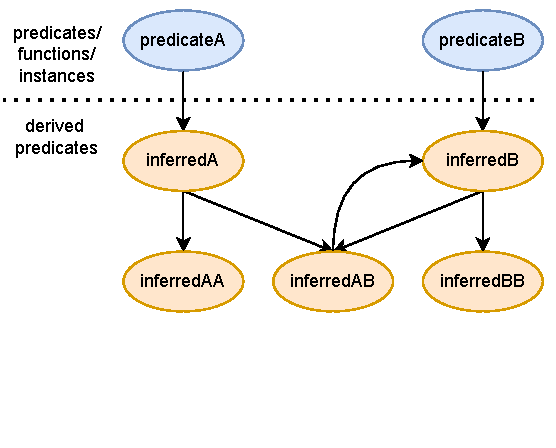
\includegraphics[width=\linewidth]{pddl/figures/derived_graph.pdf}
        \resizebox{\linewidth}{!}{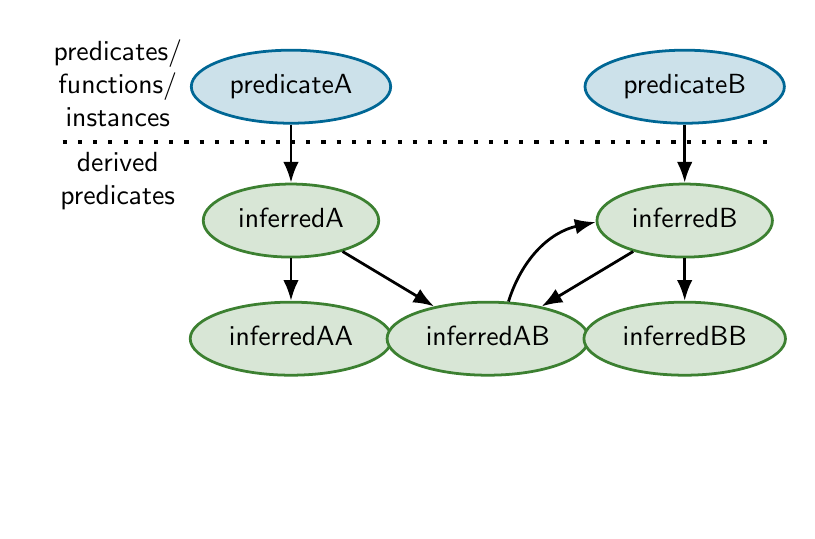
\begin{tikzpicture}[font=\sffamily]
    
    \coordinate (origin) at (0,0);
    \draw (origin) node[bubbleBlue] (predicateA) {predicateA\strut};
    
    \draw ($(predicateA) + (5,0)$) node[bubbleBlue] (predicateB) {predicateB\strut};
    
    \draw ($(predicateA) + (0,-1.7)$) node[bubbleGreen] (inferredA) {inferredA\strut};
    \draw ($(predicateB) + (0,-1.7)$) node[bubbleGreen] (inferredB) {inferredB\strut};
    
    \draw ($(inferredA) + (0,-1.5)$) node[bubbleGreen] (inferredAA) {inferredAA\strut};
    \draw ($(inferredA) + (2.5,-1.5)$) node[bubbleGreen] (inferredAB) {inferredAB\strut};
    \draw ($(inferredB) + (0,-1.5)$) node[bubbleGreen] (inferredBB) {inferredBB\strut};
    
    \phantom{\draw ($(inferredAA) + (0,-1.7)$) node[bubblePurple] (action1) {action1\strut};} % phantom for alignment with other figure
    
    \draw[arrow] (predicateA) -- (inferredA);
    \draw[arrow] (predicateB) -- (inferredB);
    
    \draw[arrow] (inferredA) -- (inferredAA);
    \draw[arrow] (inferredA) -- (inferredAB);
    \draw[arrow] (inferredB) -- (inferredAB);
    \draw[arrow] (inferredB) -- (inferredBB);
    
    \draw[arrow] (inferredAB) to [bend left] (inferredB);
    
    % labels
    \draw ($(predicateA) + (-2.2,0)$) node (topLabel) {\begin{tabular}{c}
            predicates/\\
            functions/\\
            instances
    \end{tabular}};

    \draw ($(topLabel) + (0,-1.2)$) node (botLabel) {\begin{tabular}{c}
            derived\\
            predicates
    \end{tabular}};
    
    % dotted line
    \draw[loosely dotted,
        draw=black, 
        line width=1.5pt] ($(topLabel) + (-0.7,-0.7)$) -- ++ (9,0);
    
    
\end{tikzpicture}}
        \caption{Complete graph.}%
        \label{planta:fig:derived_graph}
    \end{subfigure}
    \hfill
    \begin{subfigure}[t]{0.48\linewidth}
        \vspace{0pt} % Aligns top
        \centering
        %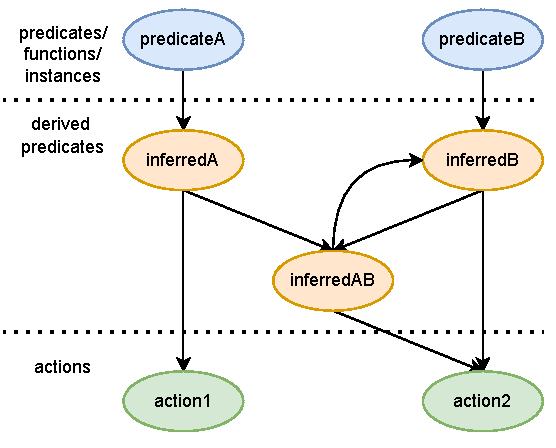
\includegraphics[width=\linewidth]{pddl/figures/derived_graph_pruned.pdf}
        \resizebox{\linewidth}{!}{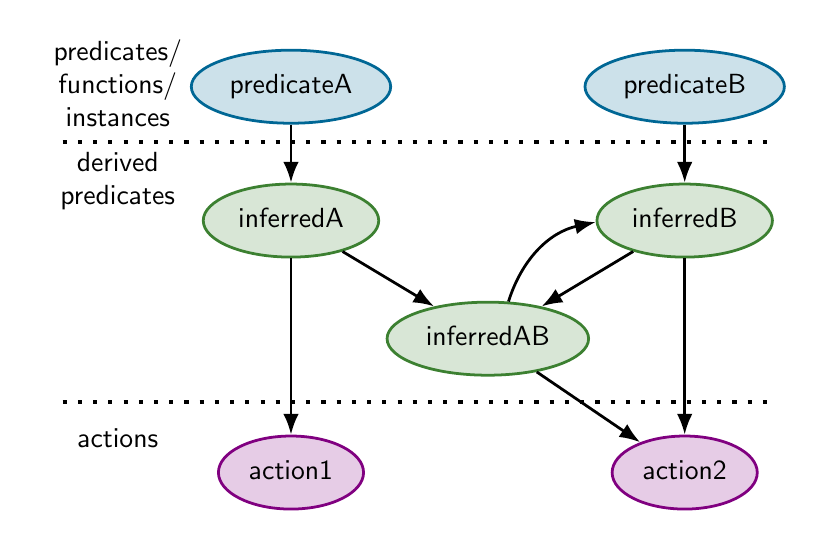
\begin{tikzpicture}[font=\sffamily]
    
    \coordinate (origin) at (0,0);
    \draw (origin) node[bubbleBlue] (predicateA) {predicateA\strut};
    
    \draw ($(predicateA) + (5,0)$) node[bubbleBlue] (predicateB) {predicateB\strut};
    
    \draw ($(predicateA) + (0,-1.7)$) node[bubbleGreen] (inferredA) {inferredA\strut};
    \draw ($(predicateB) + (0,-1.7)$) node[bubbleGreen] (inferredB) {inferredB\strut};
    
    \draw ($(inferredA) + (0,-1.5)$) node (inferredAA) {};
    \draw ($(inferredA) + (2.5,-1.5)$) node[bubbleGreen] (inferredAB) {inferredAB\strut};
    \draw ($(inferredB) + (0,-1.5)$) node (inferredBB) {};
    
    \draw ($(inferredAA) + (0,-1.7)$) node[bubblePurple] (action1) {action1\strut};
    \draw ($(inferredBB) + (0,-1.7)$) node[bubblePurple] (action2) {action2\strut};
    
    
    \draw[arrow] (predicateA) -- (inferredA);
    \draw[arrow] (predicateB) -- (inferredB);
    
    \draw[arrow] (inferredA) -- (action1);
    \draw[arrow] (inferredA) -- (inferredAB);
    \draw[arrow] (inferredB) -- (inferredAB);
    \draw[arrow] (inferredB) -- (action2);
    \draw[arrow] (inferredAB) -- (action2);
    
    \draw[arrow] (inferredAB) to [bend left] (inferredB);
    
    % labels
    \draw ($(predicateA) + (-2.2,0)$) node (topLabel) {\begin{tabular}{c}
            predicates/\\
            functions/\\
            instances
    \end{tabular}};

    \draw ($(topLabel) + (0,-1.2)$) node (midLabel) {\begin{tabular}{c}
            derived\\
            predicates
    \end{tabular}};

    \draw ($(topLabel) + (0,-4.5)$) node (botLabel) {\begin{tabular}{c}
            actions
    \end{tabular}};
    
    % dotted line
    \draw[loosely dotted,
        draw=black, 
        line width=1.5pt] ($(topLabel) + (-0.7,-0.7)$) -- ++ (9,0);
        
   \draw[loosely dotted,
   draw=black, 
   line width=1.5pt] ($(botLabel) + (-0.7,0.5)$) -- ++ (9,0);
    
    
\end{tikzpicture}}
        \caption{Pruned graph for $\pi=(\texttt{action1}, \texttt{action2})$.}%
        \label{planta:fig:pruned_graph}
    \end{subfigure}
    \caption{Derived predicates resolution graphs for the PDDL formulation in \Cref{planta:lst:example_derived}: (a) the full dependency graph and (b) the pruned graph for the plan $\pi = (\texttt{action1}, \texttt{action2})$. The predicates $\texttt{predicateAA}$ and $\texttt{predicateC}$ are omitted to simplify the visualization, as they are not relevant to the graph structure due to having no child predicates.}%
    \label{planta:fig:derived_graphs_combined}
\Description{Two directed dependency graphs, with arrows pointing from a predicate to predicates or
actions that depend on it. In the complete graph on the left, \texttt{predicateA} leads
to \texttt{inferredA}, which leads to \texttt{inferredAA} and \texttt{inferredAB}.
PredicateB leads to \texttt{inferredB}, which leads to \texttt{inferredAB} and
\texttt{inferredBB}. InferredAB also points back to \texttt{inferredB}, forming a cycle.
In the pruned graph on the right, \texttt{inferredAA} and \texttt{inferredBB} are
removed. \texttt{action1} depends on \texttt{inferredA}, and \texttt{action2} depends on
\texttt{inferredB} and \texttt{inferredAB}. The cycle is retained.}
\end{figure}

To solve derived predicates, this work introduces \Cref{planta:S-alg:solve_derived}. It partitions the resolution graph into strongly connected components~(SCCs) using Tarjan's algorithm~\cite{doi:10.1137/0201010}, which separates acyclic from cyclic components. The acyclic components are resolved in topological order, while the cyclic components are resolved using a fixed-point iteration. Root nodes are considered solved by definition, as they correspond to non-derived predicates. For instance, in the graph shown in \Cref{planta:fig:derived_graph}, the derived predicates $\texttt{inferredB}$ and $\texttt{inferredAB}$ form a cycle, whereas the other derived predicates are acyclic.

\paragraph{Apply action effects algorithm}

With the addition of derived predicates, applying an action's effects can invalidate previously derived predicates and make new ones derivable. Instead of recomputing all derived predicates, this work exploits the structure of the derived predicates graph to re-evaluate only the derived predicates that depend on the predicates modified by the effects (\Cref{planta:S-alg:apply_new}). For example, in the PDDL domain described in \Cref{planta:lst:example_derived}, applying the action $(\texttt{action1}~\texttt{instance1})$ adds $(\texttt{predicateB}~\texttt{instance1})$ to the state, which requires re-evaluating only the derived predicates $\texttt{inferredB}$, $\texttt{inferredAB}$, and $\texttt{inferredBB}$.

\paragraph{Derived graph pruning by action}

To optimize the evaluation of derived predicates during plan graph generation and runtime execution in \plansys, this work proposes appending the actions defined in the \emph{planning domain} to the derived graph and pruning it to retain only the predicates relevant to the current action plan. For example, given the \emph{planning domain} in \Cref{planta:lst:example_derived} and the plan \(\pi = (\texttt{action1}, \texttt{action2})\), the derived graph shown in \Cref{planta:fig:derived_graph} can be pruned to the graph in \Cref{planta:fig:pruned_graph}, avoiding the unnecessary resolution of predicates \(\texttt{inferredAA}\) and \(\texttt{inferredBB}\).


%%% Local Variables:
%%% mode: latex
%%% TeX-master: "main"
%%% End:

\section{Evaluation}\label{planta:sec:evaluation}

This work evaluates \acronym on two use cases from the literature: (i) the SUAVE exemplar~\cite{suave}, in which an AUV performs pipeline inspection, and (ii) an AGV scenario from Cámara et al.~\cite{CAMARASoftwareArchitectureTask2020}, in which the AGV navigates through an environment composed of corridors and rooms. The evaluation is organized around the following research questions:
\begin{description}
    \item[RQ1 (Feasibility).] Can \acronym be integrated into a ROS~2-based robotic system to perform task and architecture co-adaptation at runtime, and how does its mission performance compare with that of existing managing subsystems?
    \item[RQ2 (Performance efficiency).] How do \acronym's planning time and peak memory usage compare with those of the approach by Cámara et al.~\cite{CAMARASoftwareArchitectureTask2020}, and does \acronym produce plans of comparable quality?
    \item[RQ3 (Scalability).] How does \acronym's planning time evolve as the mission and adaptation spaces grow, and what are the trade-offs between optimal and satisficing planning?
\end{description}
RQ1 is addressed by the implementation of \acronym and its integration with \plansys~(\Cref{planta:sec:implementation}), and by applying \acronym to the SUAVE exemplar and its TACA extension~(\Cref{planta:sec:suave_exp}), which primarily serve as a feasibility evaluation. RQ2 is addressed with the AGV scenario~(\Cref{planta:sec:nav_exp}). RQ3 is addressed by varying the AGV scenario along four dimensions, independently and in combination~(\Cref{planta:sec:scale_exp}). For all scenarios, the size of the planning instance is reported in terms of the number of task and reconfiguration actions, derived predicates, objects, and initial facts, to characterize the complexity of \acronym's planning formulations~(\Cref{planta:tab:pddl_instances}). The complete source code and experimental artifacts are publicly available online for the SUAVE experiments~\cite{gustavo_rezende_2026_23619542} and the navigation experiments~\cite{gustavo_rezende_2026_23647225}.

\begin{table}[tbp]
\centering
\caption{Complexity of the planning instances.
    \emph{Task actions}: PDDL actions encoding each task in the mission.
    \emph{Reconfig.\ actions}: PDDL actions encoding architecture reconfiguration.
    \emph{Objects}: domain constants and problem-instance objects.
    \emph{Init.\ facts}: ground atoms in the initial state.
    \emph{Derived predicates}: predicates generated by \owltopddl from the ontology.
    The scalability instances are reported at the maximum tested parameter value
    (\Sone: 900 nodes, \Stwo: 15 architectural configurations, \Sthree: 4 corridor types,
    \Sfour: 5 mission-level actions, and \Sfive: 90 nodes).}%
\label{planta:tab:pddl_instances}
\begin{tabular}{lccccc}
\toprule
\textbf{Scenario} & \makecell{\textbf{Task}\\\textbf{actions}} & \makecell{\textbf{Reconfig.}\\\textbf{actions}} & \textbf{Objects} & \makecell{\textbf{Init.}\\\textbf{facts}} & \makecell{\textbf{Derived}\\\textbf{predicates}} \\ \midrule
SUAVE          & 3 & 2 & 44  & 115  & 54 \\
SUAVE extended & 4 & 2 & 49  & 125  & 55 \\ \midrule
Navigation     & 1 & 2 & 537 & 3184 & 53 \\
\Sone          & 1 & 2 & 947 & 8878 & 53 \\
\Stwo          & 1 & 2 & 150 & 1012 & 53 \\
\Sthree        & 1 & 2 & 144 & 1561 & 53 \\
\Sfour         & 5 & 2 & 153 & 988  & 53 \\
\Sfive         & 5 & 2 & 173 & 1635 & 53 \\
\bottomrule
\end{tabular}
\end{table}

\subsection{SUAVE exemplar}\label{planta:sec:suave_exp}
\paragraph{Experimental design}
To assess \acronym's feasibility, mission performance, and reaction time, it is applied to the SUAVE exemplar~(see \Cref{planta:sec:running_example}) and its TACA extension.

To support the benchmarking of different adaptation approaches, the SUAVE system is structured into a managing and a managed subsystem. The managing subsystem, responsible for the adaptation logic, can be replaced by any self-adaptive system that complies with the provided interfaces. SUAVE is packaged with three distinct managing subsystems: one that arbitrarily selects configurations, a behavior tree-based one, and  Metacontrol~\cite{bozhinoski2022mros}. Additionally, Silva et al.~\cite{rosa} made a ROSA implementation of SUAVE and its extended version available.

To apply \acronym to SUAVE, this work proposes a \pddltomasys model of the SUAVE exemplar based on the SUAVE \tomasys ontology. The main differences are the addition of new actions, utility rules, and a rule to handle uncertainty \Utwo~(water visibility). First, the actions \emph{search pipeline} and \emph{inspect pipeline}, as well as their functional requirements, are added to the SUAVE ontology. For the extended use case the \emph{recharge battery} action is also included. For example, $\requiresF$ relates \emph{search pipeline} to the functions \emph{maintain motion} and \emph{generate search path}. Then, rules are added to infer the $\FunctionsTomasys$ utility, for example, a rule that instantiates the generic (utility) rule of \Cref{planta:sec:tomasys_pddl} for the \emph{generate search path} function. Finally, the following rule is defined to infer whether the \emph{generate search path} function designs are realizable, given the measured water visibility:
\begin{align*}
    &\FunctionDesign(?fd1) \wedge
    \hasQAestimation(?fd1, ?eqa) \wedge
    \isQAtype(?eqa, water\_visibility) \wedge \\
    &\qaHasValue(?eqa, ?eqav) \wedge
    \QAvalue(?mqa) \wedge
    sameAs(?mqa, obs\_water\_visibility) \wedge \\
    & \qaHasValue(?mqa, ?mqav) \wedge
    \isQAtype(?mqa, water\_visibility) \wedge
    lessThan(?mqav, ?eqav) \\
    &\implies \fdRealisability(?fd1, false)
\end{align*}

To exemplify the output of the model transformation process, \Cref{planta:lst:search_pipeline_managed} shows the final PDDL formulation for the search pipeline action from the SUAVE use case. The SUAVE task actions in \Cref{planta:tab:pddl_instances} include the non-managed action of starting the robot. The extended instance adds one extra PDDL action schema, recharge battery, and one derived predicate that encodes the battery level condition for uncertainty~\Uthree.

\paragraph{Experimental Setup}
To compare \acronym with existing adaptation approaches, it was evaluated on both the original and extended SUAVE use cases. To reduce the risk of bias from a single parameter set, as in~\cite{suave, rosa}, the evaluation used randomized values for the robot's initial position, the water visibility shift (i.e., its initial value), and the timing of thruster failures. Specifically, three experiments were conducted for each use case, each with a distinct parameter configuration as detailed in \Cref{planta:tab:suave_params}.

\begin{table}[tbp]
\centering
\caption{Parameter configuration for the SUAVE experiments, where $U(a,b)$ is a random uniform distribution from $a$ to $b$. The initial position is relative to the Gazebo reference frame, where $x$ is fixed at $-17.0$ and $z$ at $-18.5$. The time limit for each execution is set to $250$ seconds.}%
\label{planta:tab:suave_params}
\resizebox{.95\textwidth}{!}{%
\begin{tabular}{llllllll}
\toprule
\multirow{2}{*}{\textbf{Exp.}} &
  \textbf{Initial position} &
  \multicolumn{4}{l}{\textbf{Water visibility}} &
  \multicolumn{2}{l}{\textbf{Thruster failures}} \\
 &
  \textbf{Y} &
  \textbf{Min (m)} &
  \textbf{Max (m)} &
  \textbf{Period (s)} &
  \textbf{Shift (s)} &
  \textbf{Thruster} &
  \textbf{Time (s)} \\ \midrule
1 & $2.5 + U(-0.5, 0.5)$ & 2.5  & 2.5  & N/A & N/A      & 1 and 3 & $100 + U(-100, 100)$ \\
2 & $2.5 + U(-0.5, 0.5)$ & 1.25 & 3.75 & 120 & $U(0,120)$ & N/A     & N/A                \\
3 & $2.5 + U(-0.5, 0.5)$ & 1.25 & 3.75 & 120 & $U(0,120)$ & 1 and 3 & $100 + U(-100, 100)$ \\ \bottomrule
\end{tabular}%
}
\end{table}

The original use case was executed 30 times with no managing subsystem, as well as with each of the following managing subsystems: a random subsystem, a behavior-tree-based subsystem (BT), Metacontrol, ROSA, and \acronym. The extended scenario, which includes TACA, was also executed 30 times for the BT-based subsystem, ROSA, and \acronym. In both the original and the extended scenarios, Fast Downward was configured to use A* search with the blind heuristic for \acronym. To ensure that outliers were averaged out, the parameters were kept the same for each group of five runs (i.e., runs 1–5, 6–10, etc.) within the 30 runs. For each run, standard SUAVE metrics~\cite{suave} were collected: \emph{pipeline search time}, the time from mission start until the AUV locates the pipeline, and \emph{pipeline distance inspected}, the total length of pipeline inspected during the mission. A third metric, \emph{reaction time}~\cite{rosa}, was also collected: the time elapsed from a constraint violation until the managing system completes adaptation of the managed subsystem.

\paragraph{Results}
The experimental results for the SUAVE use case are presented in \Cref{planta:tab:suave_results} and for the extended use case in \Cref{planta:tab:suave_extended_results}. To verify whether there is a statistically significant difference between the results, the Wilcoxon signed-rank test was applied to all pairs of managing subsystems for both the \emph{pipeline search time} and \emph{pipeline distance inspected} metrics. The p-values for experiment 3 and extended experiment 3, which combine thruster failures and water visibility changes, are reported in \Cref{planta:tab:wilcoxon}. The p-values for the remaining experiments are reported in the electronic supplement.

Results were paired by run index, and pairs in which either system did not find the pipeline were excluded from both comparisons. For each metric, the alternative hypothesis is that the managing system in the row achieves a lower \emph{pipeline search time} or, respectively, a greater \emph{pipeline distance inspected} than the one in the column.
p-values less than 0.05 indicate statistical significance in favor of the alternative hypothesis.

% Generated by scripts/summarize_suave_results.py
% Source campaigns: /tmp/claude-1000/-home-gus-ros-workspaces-planta-ws/90f03437-a284-4a9e-9032-238a88aa72ef/scratchpad/paper_tables_input/campaigns
% Do not edit by hand.
\begin{table}[tb]
\centering
\caption{SUAVE results. The Random managing subsystem found the pipeline in 21/30 runs (70.00\%) for Experiment 1, 22/30 runs (73.33\%) for Experiment 2, and 22/30 runs (73.33\%) for Experiment 3. All other managing subsystems found the pipeline in every run. Search time and inspected distance report the mean and sample standard deviation only for runs that found the pipeline. \Uone denotes thruster failure and \Utwo water visibility. Reaction times are arithmetic means of recorded events per uncertainty across all retained runs. N/A denotes an inapplicable metric or insufficient observations. The initial visibility adjustment in Experiment 1 is excluded.}\label{planta:tab:suave_results}
\resizebox{.95\textwidth}{!}{%
\begin{tabular}{llcccccc}
\toprule
\multirow{2}{*}{\textbf{Exp.}} & \multirow{2}{*}{\textbf{Managing subsystem}} & \multicolumn{2}{c}{\textbf{Search time (s)}} & \multicolumn{2}{c}{\textbf{Distance inspected (m)}} & \multicolumn{2}{c}{\textbf{Mean reaction time (s)}} \\
 & & \textbf{Mean} & \textbf{Std.\ dev.} & \textbf{Mean} & \textbf{Std.\ dev.} & \textbf{\Uone} & \textbf{\Utwo} \\
\midrule
\multirow{6}{*}{1} & None & 58.77 & 26.07 & 49.50 & 12.56 & N/A & N/A \\
 & Random & 126.71 & 52.90 & 11.65 & 10.08 & N/A & N/A \\
 & BT & 59.63 & 27.46 & 58.17 & 8.43 & 0.07 & N/A \\
 & Metacontrol & 59.20 & 25.50 & 58.92 & 8.63 & 1.11 & N/A \\
 & ROSA & 65.33 & 27.48 & 57.76 & 9.06 & 0.75 & N/A \\
 & \textbf{\acronym} & \textbf{65.07} & \textbf{33.95} & \textbf{43.56} & \textbf{8.77} & \textbf{0.88} & \textbf{N/A} \\
\midrule
\multirow{6}{*}{2} & None & 152.13 & 30.32 & 27.31 & 11.23 & N/A & N/A \\
 & Random & 113.32 & 48.30 & 10.91 & 8.15 & N/A & N/A \\
 & BT & 83.83 & 30.96 & 50.42 & 10.25 & N/A & 0.13 \\
 & Metacontrol & 85.53 & 31.51 & 50.22 & 10.37 & N/A & 1.37 \\
 & ROSA & 89.03 & 31.19 & 49.69 & 10.46 & N/A & 1.52 \\
 & \textbf{\acronym} & \textbf{87.83} & \textbf{31.41} & \textbf{44.45} & \textbf{10.11} & \textbf{N/A} & \textbf{1.78} \\
\midrule
\multirow{6}{*}{3} & None & 148.97 & 33.14 & 25.90 & 9.47 & N/A & N/A \\
 & Random & 119.50 & 52.35 & 8.76 & 7.31 & N/A & N/A \\
 & BT & 84.43 & 30.94 & 49.82 & 10.30 & 0.07 & 0.12 \\
 & Metacontrol & 86.77 & 31.48 & 49.30 & 10.08 & 1.22 & 1.52 \\
 & ROSA & 89.57 & 31.71 & 49.31 & 10.53 & 0.78 & 1.56 \\
 & \textbf{\acronym} & \textbf{88.73} & \textbf{32.07} & \textbf{43.58} & \textbf{9.45} & \textbf{1.45} & \textbf{1.86} \\
\bottomrule
\end{tabular}%
}
\end{table}


% Generated by scripts/summarize_suave_results.py
% Source campaigns: /tmp/claude-1000/-home-gus-ros-workspaces-planta-ws/90f03437-a284-4a9e-9032-238a88aa72ef/scratchpad/paper_tables_input/campaigns
% Do not edit by hand.
\begin{table}[tb]
\centering
\caption{SUAVE extended results. All managing subsystems found the pipeline in every run. Search time and inspected distance report the mean and sample standard deviation only for runs that found the pipeline. \Uone denotes thruster failure and \Utwo water visibility, with \Uthree denoting battery level. Reaction times are arithmetic means of recorded events per uncertainty across all retained runs. N/A denotes an inapplicable metric or insufficient observations. The initial visibility adjustment in Experiment 1 is excluded.}\label{planta:tab:suave_extended_results}
\resizebox{.95\textwidth}{!}{%
\begin{tabular}{llccccccc}
\toprule
\multirow{2}{*}{\textbf{Exp.}} & \multirow{2}{*}{\textbf{Managing subsystem}} & \multicolumn{2}{c}{\textbf{Search time (s)}} & \multicolumn{2}{c}{\textbf{Distance inspected (m)}} & \multicolumn{3}{c}{\textbf{Mean reaction time (s)}} \\
 & & \textbf{Mean} & \textbf{Std.\ dev.} & \textbf{Mean} & \textbf{Std.\ dev.} & \textbf{\Uone} & \textbf{\Utwo} & \textbf{\Uthree} \\
\midrule
\multirow{3}{*}{1} & BT & 64.30 & 34.37 & 23.40 & 8.17 & 0.09 & N/A & 1.09 \\
 & ROSA & 61.10 & 24.85 & 22.41 & 6.95 & 0.81 & N/A & 1.95 \\
 & \textbf{\acronym} & \textbf{71.47} & \textbf{37.23} & \textbf{17.47} & \textbf{8.79} & \textbf{0.89} & \textbf{N/A} & \textbf{1.44} \\
\midrule
\multirow{3}{*}{2} & BT & 83.93 & 30.88 & 16.74 & 9.09 & N/A & 0.12 & 1.08 \\
 & ROSA & 88.70 & 31.50 & 15.40 & 8.96 & N/A & 1.57 & 2.03 \\
 & \textbf{\acronym} & \textbf{88.20} & \textbf{31.86} & \textbf{14.72} & \textbf{8.44} & \textbf{N/A} & \textbf{2.37} & \textbf{2.25} \\
\midrule
\multirow{3}{*}{3} & BT & 89.07 & 40.14 & 16.25 & 9.07 & 0.07 & 0.12 & 1.07 \\
 & ROSA & 88.10 & 31.71 & 15.48 & 8.96 & 0.76 & 1.67 & 1.96 \\
 & \textbf{\acronym} & \textbf{89.30} & \textbf{32.06} & \textbf{14.29} & \textbf{8.47} & \textbf{1.57} & \textbf{2.40} & \textbf{2.31} \\
\bottomrule
\end{tabular}%
}
\end{table}


\begin{table}[tbp]
\centering
\caption{Paired Wilcoxon signed-rank comparisons for experiment 3 and extended experiment 3. Each cell reports the unadjusted p-values for the comparison between the managing subsystem in the row and the one in the column for both the \emph{pipeline search time} and \emph{pipeline distance inspected} metrics. Cells with a green background indicate that the alternative hypothesis was favored, and cells with a blue background indicate that the null hypothesis cannot be rejected in favor of the alternative hypothesis. Values rounding to 0.000 are shown as $<0.001$. ``MC'' stands for Metacontrol.}%
\label{planta:tab:wilcoxon}
\begin{subtable}{\textwidth}
\centering
\inputtablebody{pddl/tables/wilcoxon_analysis/exp3_wilcoxon.tex}
\caption{Experiment 3}\label{planta:tab:wilcoxon-exp3}
\end{subtable}

\medskip
% 0.78 matches the font size of (a): the generated table scales to 0.7\textwidth
\begin{subtable}{0.78\textwidth}
\centering
\inputtablebody{pddl/tables/wilcoxon_analysis/extended_exp3_wilcoxon.tex}
\caption{Extended experiment 3}\label{planta:tab:wilcoxon-extended-exp3}
\end{subtable}
\end{table}

\emph{SUAVE experiments:} Across the three SUAVE experiments (\Cref{planta:tab:wilcoxon-exp3} and \Cref{planta:S-tab:wilcoxon-exp1,planta:S-tab:wilcoxon-exp2}), the BT managing subsystem achieved significantly lower \emph{pipeline search times} than all other configurations. Metacontrol achieved significantly lower search times than ROSA and \acronym in every experiment. \acronym achieved significantly lower search times than ROSA in experiment 2, while no statistically significant difference between them was detected in experiments 1 and 3. For \emph{pipeline distance inspected}, BT, Metacontrol, and ROSA each achieved significantly greater distances than \acronym in all three experiments. \acronym achieved significantly greater inspected distances than Random in every experiment. Compared with the configuration without a managing subsystem, \acronym inspected significantly less pipeline distance in experiment 1 and significantly more in experiments 2 and 3. % chktex 12 -- sentence starts with a macro

\emph{SUAVE extended experiments:} Across the three extended SUAVE experiments (\Cref{planta:tab:wilcoxon-extended-exp3} and \Cref{planta:S-tab:wilcoxon-extended-exp1,planta:S-tab:wilcoxon-extended-exp2}), the BT managing subsystem achieved significantly lower \emph{pipeline search times} than ROSA and \acronym, while no statistically significant difference in search time was detected between ROSA and \acronym. For \emph{pipeline distance inspected}, BT achieved significantly greater distances than both ROSA and \acronym, and ROSA achieved significantly greater distances than \acronym in every experiment.

\emph{Answer to RQ1:} These results support the feasibility of using \acronym for runtime task and architecture co-adaptation in SUAVE, but also reveal limitations in mission performance. BT, Metacontrol, and ROSA each achieved significantly better results than \acronym on at least one metric in every experiment in which they were evaluated. \acronym performed significantly better than Random on both metrics in all original experiments, and better than the configuration without a managing subsystem in experiments 2 and 3, but worse in experiment 1. BT's shorter mean reaction times (\Cref{planta:tab:suave_results,planta:tab:suave_extended_results}) may partly explain its advantage, although the experiments do not establish a causal relationship between reaction time and mission performance. % chktex 12 -- sentence starts with a macro

\subsection{Navigation use case}\label{planta:sec:nav_exp}
\paragraph{Experimental design}
To evaluate \acronym's performance efficiency, in terms of planning time and peak resident set size (RSS) memory usage, and its plan quality, it was applied to the navigation scenario from~\cite{CAMARASoftwareArchitectureTask2020}. Results were compared to those obtained from a replicated implementation of the algorithm proposed in~\cite{CAMARASoftwareArchitectureTask2020}, hereafter referred to as \CamaraApproach.

In the scenario, a robot must navigate from an initial position to a goal position within an environment composed of corridors and rooms. Some corridors might be dark or contain obstacles, reducing their safety. During navigation, the robot dynamically adapts both its architecture (i.e., the sensors and localization algorithms employed) and its task execution (i.e., the path followed) to circumvent failures or prioritize safety or energy consumption. For example, if the robot's planned path includes a dark corridor and its lamp fails during execution, it must reconfigure its architecture and adapt its task execution to avoid dark corridors.

\paragraph{Experimental setup}

To compare \acronym's time performance and memory usage with \CamaraApproach, the map from~\cite{CAMARASoftwareArchitectureTask2020} was discretized to ensure uniform edge lengths. This change was necessary because \acronym does not support numeric fluents and therefore cannot handle edges of varying sizes~(\Cref{planta:sec:limitations}).
\acronym was then applied to perform task and configuration planning on the discretized map. For this comparison, Fast Downward was configured to use eager greedy search with the goal-count heuristic.

Additionally, a model generator was developed to produce PRISM models equivalent to those used in the final step of \CamaraApproach\footnote{The complete algorithm from~\cite{CAMARASoftwareArchitectureTask2020} could not be replicated.}, enabling policy generation for task planning and reconfiguration. A minor correction was introduced to the original PRISM model by adding an effect to the move actions, allowing the selection of distinct configurations for each corridor.  This work assumes that the correction aligns with the authors’ original intent, as the published model appears to contain a typographical error. For all experiments, PRISM was executed with the goal of maximizing the amount of battery remaining at the end of the mission. Both approaches were evaluated by applying them ten times to all possible combinations of initial and goal locations.

\paragraph{Results}
\Cref{planta:fig:camara_pddl_sas} shows that, at the median, \acronym generates both task and configuration plans $3.00$ times faster than \CamaraApproach generates the corresponding policy from the PRISM models, with $6.84$ times smaller peak memory usage. In the scenarios with the worst planning time, \acronym (from location 16 to 25) takes $0.56$ seconds with $66.88$~MiB peak memory usage, compared to $13.71$ seconds with $4089.03$~MiB peak memory usage for \CamaraApproach (from location 52 to 24). Notably, the spread of execution times and memory consumption is much higher for \CamaraApproach, making the resources required by \acronym more predictable. These results should be interpreted as a comparison of the computational cost of two different ways of addressing TACA rather than as a direct comparison of approaches that pursue the same objective. \CamaraApproach seeks an optimal task and configuration policy under probabilistic uncertainty, whereas \acronym favors satisficing planning over mission-level optimality, planning from the currently observed state and handling changes during execution through replanning. % chktex 12 -- sentence starts with a macro

Despite the difference in planning time and memory usage, the two approaches produce plans with almost identical path length and remaining battery. The distributions of distance traveled and of the numbers of move and reconfiguration actions nearly coincide. For example, the interquartile range of distance traveled is $36.81$ to $82.70$ for \acronym and $36.62$ to $82.66$ for \CamaraApproach, with the same median of $59.89$. The median remaining battery differs by only $1.02\%$ ($25219.50$ for \acronym against $25480.00$ for \CamaraApproach). Both approaches reconfigure more than once in a minority of the scenarios, $11.85\%$ for \acronym and $15.52\%$ for \CamaraApproach, and up to four times (for example, between locations 11 and 17 for \acronym and between locations 5 and 18 for \CamaraApproach). % chktex 12 -- sentence starts with a macro

\begin{figure}[tbp]
    \centering
    \hfill
    \begin{subfigure}[t]{0.45\linewidth}
        \vspace{0pt} % Aligns top
        \centering
        \input{pddl/navigation_experiment/data/camara_map_prism_experiment_time_boxstats.tex}%
\input{pddl/navigation_experiment/data/camara_map_pddl_experiment_time_boxstats.tex}%
% Generated by navigation_planta; do not edit by hand.
\begin{tikzpicture}[baseline=(paperAxis.north)]
\begin{axis}[name=paperAxis,
width=\textwidth,
height=0.75\textwidth,
boxplot/draw direction=y,
xmin=0,
xmax=3,
xtick={1,2},
xticklabels={\CamaraApproach,\paperEagerLabel},
ylabel={Planning time [s]},
ymajorgrids=true,
ymode=log,
ymin=0.3,
ymax=30,
ytick={1,10},
extra y ticks={0.5,30},
extra y tick labels={0.5,30}
]
\addplot+[boxplot prepared={lower whisker=\camaraPrismTimeLW,lower quartile=\camaraPrismTimeLQ,median=\camaraPrismTimeMED,upper quartile=\camaraPrismTimeUQ,upper whisker=\camaraPrismTimeUW,draw position=1,box extend=0.2},draw=\blueColor,fill=\blueColor!30,line width=0.75pt,mark=o,mark options={fill=\blueColor,draw=\blueColor,opacity=0.2,line width=0.5pt}] table[y=y,col sep=comma] {pddl/navigation_experiment/data/camara_map_prism_experiment_time_outliers.csv}
node[left,text=\blueColor] at (boxplot box cs: \camaraPrismTimeMED,0) {\pgfmathprintnumber{\camaraPrismTimeMED}};
\addplot+[boxplot prepared={lower whisker=\camaraPddlTimeLW,lower quartile=\camaraPddlTimeLQ,median=\camaraPddlTimeMED,upper quartile=\camaraPddlTimeUQ,upper whisker=\camaraPddlTimeUW,draw position=2,box extend=0.2},draw=\greenColor,fill=\greenColor!30,line width=0.75pt,mark=o,mark options={fill=\greenColor,draw=\greenColor,opacity=0.2,line width=0.5pt}] table[y=y,col sep=comma] {pddl/navigation_experiment/data/camara_map_pddl_experiment_time_outliers.csv}
node[left,text=\greenColor] at (boxplot box cs: \camaraPddlTimeMED,0) {\pgfmathprintnumber{\camaraPddlTimeMED}};
\end{axis}
\end{tikzpicture}

        \caption{Planning time comparison between \acronym and \CamaraApproach.}%
        \label{planta:fig:time_comparison}
    \end{subfigure}
    \hfill
    \begin{subfigure}[t]{0.45\linewidth}
        \vspace{0pt} % Aligns top
        \centering
        \input{pddl/navigation_experiment/data/camara_map_prism_experiment_peak_memory_boxstats.tex}%
\input{pddl/navigation_experiment/data/camara_map_pddl_experiment_peak_memory_boxstats.tex}%
% Generated by navigation_planta; do not edit by hand.
\begin{tikzpicture}[baseline=(paperAxis.north)]
\begin{axis}[name=paperAxis,
width=\textwidth,
height=0.75\textwidth,
boxplot/draw direction=y,
xmin=0,
xmax=3,
xtick={1,2},
xticklabels={\CamaraApproach,\paperEagerLabel},
ylabel={RSS Peak Memory [MiB]},
ymajorgrids=true,
ymode=log,
ymin=5,
ymax=10000,
ytick={10,100,1000,10000}
]
\addplot+[boxplot prepared={lower whisker=\camaraPrismMemLW,lower quartile=\camaraPrismMemLQ,median=\camaraPrismMemMED,upper quartile=\camaraPrismMemUQ,upper whisker=\camaraPrismMemUW,draw position=1,box extend=0.2},draw=\blueColor,fill=\blueColor!30,line width=0.75pt,mark=o,mark options={fill=\blueColor,draw=\blueColor,opacity=0.2,line width=0.5pt}] table[y=y,col sep=comma] {pddl/navigation_experiment/data/camara_map_prism_experiment_peak_memory_outliers.csv}
node[left,text=\blueColor] at (boxplot box cs: \camaraPrismMemMED,0) {\pgfmathprintnumber{\camaraPrismMemMED}};
\addplot+[boxplot prepared={lower whisker=\camaraPddlMemLW,lower quartile=\camaraPddlMemLQ,median=\camaraPddlMemMED,upper quartile=\camaraPddlMemUQ,upper whisker=\camaraPddlMemUW,draw position=2,box extend=0.2},draw=\greenColor,fill=\greenColor!30,line width=0.75pt,mark=o,mark options={fill=\greenColor,draw=\greenColor,opacity=0.2,line width=0.5pt}] table[y=y,col sep=comma] {pddl/navigation_experiment/data/camara_map_pddl_experiment_peak_memory_outliers.csv}
node[left,text=\greenColor] at (boxplot box cs: \camaraPddlMemMED,0) {\pgfmathprintnumber{\camaraPddlMemMED}};
\end{axis}
\end{tikzpicture}

        \caption{Peak RSS memory comparison between \acronym and \CamaraApproach.}%
        \label{planta:fig:memory_comparison}
    \end{subfigure}
    \hfill
    \caption{Comparison between \acronym and \CamaraApproach. The number is the median value, the boxes show interquartile range (Q1--Q3), the whiskers reach until $\pm 1.5$~IQR, and the circles show a sample of the observations beyond the whiskers.}%
    \label{planta:fig:camara_pddl_sas}
\Description{Two box-plot panels compare the replicated approach \CamaraApproach with \acronym. The
left panel shows planning time in seconds, with medians of 1.21 for the replicated
approach and 0.40 for \acronym. The right panel shows peak memory in MiB, with
medians of 461.09 and 67.39, respectively. The replicated approach has a wider spread
and larger high-value outliers in both panels.}
\end{figure}

The reported computational performance difference likely underestimates \acronym's advantage. In~\cite{CAMARASoftwareArchitectureTask2020}, the final step, the sole component that could be reproduced for \CamaraApproach, accounts for only 39.34\% of the total execution time. Furthermore, \CamaraApproach generates and verifies PRISM models for the ten best paths between the initial and goal locations, selecting the best policy according to a predefined utility function. In contrast, the experiment described in this paper generates and verifies a PRISM model only for the single best path.

\emph{Answer to RQ2:} In the evaluated AGV scenario, \acronym addresses TACA at a lower computational cost than the replicated final step of \CamaraApproach, in both planning time and peak memory usage, while producing plans with almost identical path length and remaining battery.

\subsection{Scalability}\label{planta:sec:scale_exp}

\paragraph{Experimental design} To assess the scalability of the proposed approach with respect to mission and adaptation spaces, in terms of planning time and memory usage, five additional experiments were conducted using variations of the previous navigation scenario. Specifically, four experiments were designed to independently evaluate the effect of varying the map size, the number of architectural configurations, the number of quality requirements, and the number of task actions. A fifth experiment was designed to stress-test the approach by varying the map size while fixing all other parameters at their maximum values.

Furthermore, to isolate the effect of the adaptation logic on planning time and memory usage, each of the scalability experiments described above was also conducted using only the mission logic (i.e., without reconfiguration). In addition, to compare optimal and satisficing planning, all scalability experiments, both with and without the adaptation logic, were repeated with Fast Downward configured to use A* search with the blind heuristic and eager greedy search with the goal-count heuristic, where an optimal plan corresponds to the shortest plan since all actions have unit cost.

\paragraph{Experimental setup}

For each scalability experiment, a map generator produces grid-like maps with the required number of nodes, edges, and corridor types. The generator skips $10\%$ of nodes and $15\%$ of the edges are removed while preserving graph connectivity. In the baseline maps, $25\%$ of the corridors are marked as dark and $25\%$ are marked as unsafe. The generated map is then translated into a PDDL problem file, leveraging the Unified Planning~\cite{unified_planning_2025_micheli} library, with node $0$ as the robot's initial position and the highest-indexed node as the goal waypoint. \Cref{planta:fig:grid_map_example} shows an example map. Each experiment is repeated $10$ times for each search strategy~(i.e., A* and eager greedy) and adaptation mode~(with and without adaptation), while the \emph{planning time}, \emph{peak memory usage}, and the \emph{number of actions} in the plan are collected.

\begin{figure}[tbp]
    \centering
    \resizebox{0.30\textwidth}{!}{
        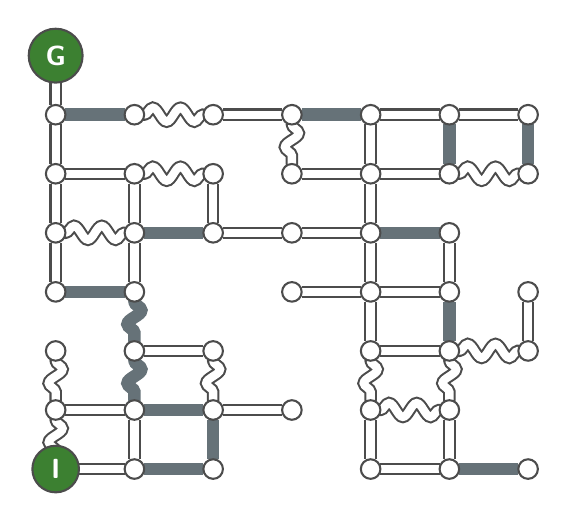
\begin{tikzpicture}[font=\sffamily\bfseries]
    
    % Create a 5x5 grid of nodes
    \foreach \i in {0,1,2,3,4,5,6} {
        \foreach \j in {0,1,2,3,4,5,6} {
            % Name each node with its coordinates
            \node at (\i, -0.75*\j) (node-\i-\j) {};
            \node[gridNode] at (\i, -0.75*\j)  {};
        }
    }
    
    \node[goal] at (0, 0.75) (goal) {G};
    
    \node[start] at (node-0-6) (start) {I};
    
    % hide deleted nodes
    
    \node[hideNode] at (node-2-3) {};
    \node[hideNode] at (node-3-4) {};
    \node[hideNode] at (node-3-6) {};
    \node[hideNode] at (node-6-2) {};
    \node[hideNode] at (node-6-5) {};
    
    
    \begin{pgfonlayer}{background}
        % colums
        \draw[corridor] (goal.center) -- (node-0-0);
        
        \draw[corridor] (node-0-0) -- (node-0-1);
        \draw[corridor] (node-0-1) -- (node-0-2);
        \draw[corridor] (node-0-2) -- (node-0-3);
        %\draw[corridor] (node-0-3) -- (node-0-4);
        \draw[corridorUnsafe] (node-0-4) -- (node-0-5);
        \draw[corridorUnsafe] (node-0-5) -- (node-0-6);
        
        %\draw[corridor] (node-1-0) -- (node-1-1);
        \draw[corridor] (node-1-1) -- (node-1-2);
        \draw[corridor] (node-1-2) -- (node-1-3);
        \draw[corridorDarkUnsafe] (node-1-3) -- (node-1-4);
        \draw[corridorDarkUnsafe] (node-1-4) -- (node-1-5);
        \draw[corridor] (node-1-5) -- (node-1-6);
        
        %\draw[corridor] (node-2-0) -- (node-2-1);
        \draw[corridor] (node-2-1) -- (node-2-2);
        %\draw[corridor] (node-2-2) -- (node-2-3);
        %\draw[corridor] (node-2-3) -- (node-2-4);
        \draw[corridorUnsafe] (node-2-4) -- (node-2-5);
        \draw[corridorDark] (node-2-5) -- (node-2-6);
        
        \draw[corridorUnsafe] (node-3-0) -- (node-3-1);
        %\draw[corridor] (node-3-1) -- (node-3-2);
        %\draw[corridor] (node-3-2) -- (node-3-3);
        %\draw[corridor] (node-3-3) -- (node-3-4);
        %\draw[corridor] (node-3-4) -- (node-3-5);
        %\draw[corridor] (node-3-5) -- (node-3-6);
        
        \draw[corridor] (node-4-0) -- (node-4-1);
        \draw[corridor] (node-4-1) -- (node-4-2);
        \draw[corridor] (node-4-2) -- (node-4-3);
        \draw[corridor] (node-4-3) -- (node-4-4);
        \draw[corridorUnsafe] (node-4-4) -- (node-4-5);
        \draw[corridor] (node-4-5) -- (node-4-6);
        
        \draw[corridorDark] (node-5-0) -- (node-5-1);
        %\draw[corridor] (node-5-1) -- (node-5-2);
        \draw[corridor] (node-5-2) -- (node-5-3);
        \draw[corridorDark] (node-5-3) -- (node-5-4);
        \draw[corridorUnsafe] (node-5-4) -- (node-5-5);
        \draw[corridor] (node-5-5) -- (node-5-6);
        
        \draw[corridorDark] (node-6-0) -- (node-6-1);
        %\draw[corridor] (node-6-1) -- (node-6-2);
        %\draw[corridor] (node-6-2) -- (node-6-3);
        \draw[corridor] (node-6-3) -- (node-6-4);
        %\draw[corridor] (node-6-4) -- (node-6-5);
        %\draw[corridor] (node-6-5) -- (node-6-6);
        
        % rows
        \draw[corridorDark] (node-0-0) -- (node-1-0);
        \draw[corridorUnsafe] (node-1-0) -- (node-2-0);
        \draw[corridor] (node-2-0) -- (node-3-0);
        \draw[corridorDark] (node-3-0) -- (node-4-0);
        \draw[corridor] (node-4-0) -- (node-5-0);
        \draw[corridor] (node-5-0) -- (node-6-0);
        
        \draw[corridor] (node-0-1) -- (node-1-1);
        \draw[corridorUnsafe] (node-1-1) -- (node-2-1);
        %\draw[corridor] (node-2-1) -- (node-3-1);
        \draw[corridor] (node-3-1) -- (node-4-1);
        \draw[corridor] (node-4-1) -- (node-5-1);
        \draw[corridorUnsafe] (node-5-1) -- (node-6-1);
        
        \draw[corridorUnsafe] (node-0-2) -- (node-1-2);
        \draw[corridorDark] (node-1-2) -- (node-2-2);
        \draw[corridor] (node-2-2) -- (node-3-2);
        \draw[corridor] (node-3-2) -- (node-4-2);
        \draw[corridorDark] (node-4-2) -- (node-5-2);
        %\draw[corridor] (node-5-2) -- (node-6-2);
        
        \draw[corridorDark] (node-0-3) -- (node-1-3);
        %\draw[corridor] (node-1-3) -- (node-2-3);
        %\draw[corridor] (node-2-3) -- (node-3-3);
        \draw[corridor] (node-3-3) -- (node-4-3);
        \draw[corridor] (node-4-3) -- (node-5-3);
        %\draw[corridor] (node-5-3) -- (node-6-3);
        
        %\draw[corridor] (node-0-4) -- (node-1-4);
        \draw[corridor] (node-1-4) -- (node-2-4);
        %\draw[corridor] (node-2-4) -- (node-3-4);
        %\draw[corridor] (node-3-4) -- (node-4-4);
        \draw[corridor] (node-4-4) -- (node-5-4);
        \draw[corridorUnsafe] (node-5-4) -- (node-6-4);
        
        \draw[corridor] (node-0-5) -- (node-1-5);
        \draw[corridorDark] (node-1-5) -- (node-2-5);
        \draw[corridor] (node-2-5) -- (node-3-5);
        %\draw[corridor] (node-3-5) -- (node-4-5);
        \draw[corridorUnsafe] (node-4-5) -- (node-5-5);
        %\draw[corridor] (node-5-5) -- (node-6-5);
        
        \draw[corridor] (node-0-6) -- (node-1-6);
        \draw[corridorDark] (node-1-6) -- (node-2-6);
        %\draw[corridor] (node-2-6) -- (node-3-6);
        %\draw[corridor] (node-3-6) -- (node-4-6);
        \draw[corridor] (node-4-6) -- (node-5-6);
        \draw[corridorDark] (node-5-6) -- (node-6-6);
   \end{pgfonlayer}
    
\end{tikzpicture}
    }
    \caption{Grid map example with $45$ retained nodes out of $50$ generated nodes.
    White edges represent normal corridors, filled edges represent dark corridors and curved edges represent unsafe corridors. The initial location is marked with {\sffamily\bfseries I} and the goal location is marked with {\sffamily\bfseries G}.
    }%
    \label{planta:fig:grid_map_example}
\Description{Grid-like navigation graph with 45 locations, consisting of a seven-by-seven grid with five locations removed and an additional goal location. Several connections are omitted. The
initial location I is at the lower left, and the goal G is above the upper-left grid
location. Edges connect neighboring locations: white straight edges denote normal
corridors, filled edges denote dark corridors, and curved edges denote unsafe corridors.
Filled curved edges denote corridors that are both dark and unsafe.}
\end{figure}

\Cref{planta:tab:scalability_params} lists the parameter ranges of the five scalability experiments. Architectural configurations are combinations of sensors and localization algorithms, and \Stwo adds further combinations\footnote{The additional architectural configurations are included to increase the size of the architectural configuration space, not to model realistic selection criteria or quality-attribute trade-offs.}. \Sthree models additional quality requirements as two new corridor types: outdoor corridors ($20\%$) and dusty corridors ($20\%$). Outdoor corridors require sensors that are robust to sunlight, for example, lidars, whereas dusty corridors require sensors that are robust to floating particles, for example, RGB cameras. \Sfour adds the mission-level PDDL actions inspect, deliver, recharge, and report. The map-size upper bound in \Sfive is lower than in \Sone because \Sfive combines the largest architectural configuration space, the largest set of corridor requirements, and the largest mission-action set, which substantially increases the planning space.

\begin{table}[tbp]
  \centering
  \caption{Parameter configurations for the five scalability experiments~(S1--S5).
    Map nodes are generated nodes. The map generator skips $10\%$ of them, so the maximum of $1000$ generated nodes in S1 and $100$ in S5 corresponds to $900$ and $90$ retained nodes, respectively.
    For S4 and S5, the number of architectural configurations grows with the number of action types: each additional mission-level PDDL action introduces two further configurations.
  }%
  \label{planta:tab:scalability_params}
  \begin{tabular}{llcccc}
    \toprule
    & \textbf{Experiment} &
    \makecell{\textbf{Map nodes}} &
    \makecell{\textbf{Arch.}\\\textbf{configs}} &
    \makecell{\textbf{Corridor}\\\textbf{types}} &
    \makecell{\textbf{Actions}} \\
    \midrule
    \Sone & Map size               & $10$--$1000$, step $10$ & $6$                 & $2$     & $1$ \\
    \Stwo & Arch.\ configurations  & $100$                   & $2,4,6,8,10,12,15$  & $2$     & $1$ \\
    \Sthree & Quality requirements   & $100$                   & $6$                 & $2,3,4$ & $1$ \\
    \Sfour & Mission-level actions           & $100$                   & $6$--$14$           & $2$     & $1,2,3,4,5$ \\
    \Sfive & Combined (stress test) & $10$--$100$, step $10$  & $23$                & $4$     & $5$ \\
    \bottomrule
  \end{tabular}
\end{table}

Experiments \Stwo, \Sthree, and \Sfour use maps with $100$ nodes, so that changes in planning time and memory usage can be interpreted primarily with respect to the dimension varied in each experiment rather than map size, which is evaluated separately in \Sone. \Sfive combines the action-driven configuration growth of \Sfour with the additional architectural configurations introduced in \Stwo, yielding $23$ configurations. The configurations added in \Sfour are intentionally not ranked by utility, which avoids introducing a separate utility-optimization factor into the mission-action scalability experiment. \Cref{planta:tab:pddl_instances} reports the resulting complexity of each experiment's planning instance at its maximum tested parameter value.

\paragraph{Results}

Across the five scalability experiments, the number of mission-level PDDL actions is the dominant driver of planning time, with map size as a secondary driver. Architectural configurations (\Stwo) and quality requirements (\Sthree) have a small effect on planning time. Map size (\Sone) produces a moderate increase for both search strategies, whereas increasing the number of mission-level PDDL actions (\Sfour) leads to a much larger increase, with A* search requiring more than an order of magnitude more time than eager greedy search while both strategies produce plans of similar length. This disparity becomes even more pronounced when all dimensions are combined (\Sfive), where A* search becomes impractical for online TACA, while eager greedy search remains manageable. Peak memory usage grows mainly with map size and, for A* search, with the number of mission-level PDDL actions. It ranges from $37.69$~MiB to $104.66$~MiB in \Sone and reaches $308.43$~MiB for A* search and $90.32$~MiB for eager greedy search in the largest \Sfive instances. \Cref{planta:tab:scalability_summary} summarizes the results, and \Cref{planta:fig:scalability_time} shows the planning-time trends of \Sone, \Sfour, and \Sfive. The plots for all five experiments, including plan length, are given in \Crefrange{planta:S-fig:s1_results}{planta:S-fig:s5_results} of the electronic supplement.

\begin{table}[tb]
\centering
\caption{Scalability experiment results at the maximum tested parameter value for each experiment (\Sone: 900 nodes, \Stwo: 15 architectural configurations, \Sthree: 4 corridor types, \Sfour: 5 mission-level actions, and \Sfive: 90 nodes).}\label{planta:tab:scalability_summary}
\resizebox{.75\textwidth}{!}{%
\begin{tabular}{lcccccccc}
\toprule
\multirow{3}{*}{\textbf{Exp.}} & \multicolumn{4}{c}{\textbf{A*}} & \multicolumn{4}{c}{\textbf{Eager greedy}} \\
\cmidrule(lr){2-5}\cmidrule(lr){6-9}
 & \multicolumn{2}{c}{\textbf{Planning time (s)}} & \multicolumn{2}{c}{\textbf{Plan length}} & \multicolumn{2}{c}{\textbf{Planning time (s)}} & \multicolumn{2}{c}{\textbf{Plan length}} \\
\cmidrule(lr){2-3}\cmidrule(lr){4-5}\cmidrule(lr){6-7}\cmidrule(lr){8-9}
 & \textbf{Mean} & \textbf{Std.} & \textbf{Mean} & \textbf{Std.} & \textbf{Mean} & \textbf{Std.} & \textbf{Mean} & \textbf{Std.} \\
\midrule
\Sone & 0.92 & 0.02 & 47.20 & 7.74 & 0.95 & 0.03 & 47.20 & 7.74 \\
\Stwo & 0.30 & 0.00 & 20.70 & 1.42 & 0.30 & 0.02 & 20.70 & 1.42 \\
\Sthree & 0.20 & 0.00 & 20.30 & 2.26 & 0.20 & 0.00 & 20.30 & 2.26 \\
\Sfour & 15.45 & 1.24 & 46.00 & 5.52 & 1.05 & 0.30 & 46.80 & 6.21 \\
\Sfive & 188.96 & 20.43 & 48.10 & 3.73 & 13.73 & 3.66 & 51.60 & 5.64 \\
\bottomrule
\end{tabular}%
}
\end{table}


\begin{figure}[tbp]
    \centering
    % Compact legends for the generated plots, so that the legend of (a) does not cover its curves.
    \pgfplotsset{every axis post/.append style={legend style={inner sep=1pt,row sep=-2pt}}}%
    \begin{subfigure}[t]{0.32\linewidth}
        \centering
        {% Generated plot: thin the x ticks so they do not overlap at this panel width.
        \pgfplotsset{every axis post/.append style={xtick={0,300,600,900}}}%
        % Generated by navigation_planta; do not edit by hand.
\begin{tikzpicture}[baseline=(paperAxis.north)]
\begin{axis}[name=paperAxis,
width=\textwidth,
height=0.75\textwidth,
xlabel={Number of Nodes},
ylabel={Planning Time [seconds]},
xmin=0,
xmax=900,
ymin=0,
ymax=1,
xtick={0,200,400,600,800,900},
grid=major,
legend pos=north west,
legend style={font=\footnotesize,nodes={scale=0.8,transform shape}},
legend image post style={scale=0.5}
]
\addplot[name path=upper0,draw=none,forget plot] table[x=nodes,y=mean_time_plus_std,col sep=comma] {pddl/navigation_experiment/data/s1_a_star_experiment_processed.csv};
\addplot[name path=lower0,draw=none,forget plot] table[x=nodes,y=mean_time_minus_std,col sep=comma] {pddl/navigation_experiment/data/s1_a_star_experiment_processed.csv};
\addplot[fill=\greenColor!20,fill opacity=0.3,draw=none,forget plot] fill between[of=upper0 and lower0];
\addplot[thick,color=\greenColor] table[x=nodes,y=mean_time,col sep=comma] {pddl/navigation_experiment/data/s1_a_star_experiment_processed.csv};
\addlegendentry{A* mean}
\addplot[name path=upper1,draw=none,forget plot] table[x=nodes,y=mean_time_plus_std,col sep=comma] {pddl/navigation_experiment/data/s1_eager_experiment_processed.csv};
\addplot[name path=lower1,draw=none,forget plot] table[x=nodes,y=mean_time_minus_std,col sep=comma] {pddl/navigation_experiment/data/s1_eager_experiment_processed.csv};
\addplot[fill=\blueColor!20,fill opacity=0.3,draw=none,forget plot] fill between[of=upper1 and lower1];
\addplot[thick,color=\blueColor] table[x=nodes,y=mean_time,col sep=comma] {pddl/navigation_experiment/data/s1_eager_experiment_processed.csv};
\addlegendentry{EG mean}
\addplot[name path=upper2,draw=none,forget plot] table[x=nodes,y=mean_time_plus_std,col sep=comma] {pddl/navigation_experiment/data/s1_a_star_no_sas_experiment_processed.csv};
\addplot[name path=lower2,draw=none,forget plot] table[x=nodes,y=mean_time_minus_std,col sep=comma] {pddl/navigation_experiment/data/s1_a_star_no_sas_experiment_processed.csv};
\addplot[fill=\orangeColor!20,fill opacity=0.3,draw=none,forget plot] fill between[of=upper2 and lower2];
\addplot[thick,color=\orangeColor] table[x=nodes,y=mean_time,col sep=comma] {pddl/navigation_experiment/data/s1_a_star_no_sas_experiment_processed.csv};
\addlegendentry{No adap. mean}
\end{axis}
\end{tikzpicture}
}
        \caption{\Sone: map size.}%
        \label{planta:plot:s1_planning_time}
    \end{subfigure}\hfill
    \begin{subfigure}[t]{0.32\linewidth}
        \centering
        % Generated by navigation_planta; do not edit by hand.
\begin{tikzpicture}[baseline=(paperAxis.north)]
\begin{axis}[name=paperAxis,
width=\textwidth,
height=0.75\textwidth,
xlabel={Number of mission actions},
ylabel={Planning Time [seconds]},
xmin=1,
xmax=5,
ymin=0,
ymax=18.3531757133,
xtick={1,2,3,4,5},
grid=major,
legend pos=north west,
legend style={font=\footnotesize,nodes={scale=0.8,transform shape}},
legend image post style={scale=0.5}
]
\addplot[name path=upper0,draw=none,forget plot] table[x=m,y=mean_time_plus_std,col sep=comma] {pddl/navigation_experiment/data/s4_astar_experiment_processed.csv};
\addplot[name path=lower0,draw=none,forget plot] table[x=m,y=mean_time_minus_std,col sep=comma] {pddl/navigation_experiment/data/s4_astar_experiment_processed.csv};
\addplot[fill=\greenColor!20,fill opacity=0.3,draw=none,forget plot] fill between[of=upper0 and lower0];
\addplot[thick,color=\greenColor] table[x=m,y=mean_time,col sep=comma] {pddl/navigation_experiment/data/s4_astar_experiment_processed.csv};
\addlegendentry{A* mean}
\addplot[name path=upper1,draw=none,forget plot] table[x=m,y=mean_time_plus_std,col sep=comma] {pddl/navigation_experiment/data/s4_eager_experiment_processed.csv};
\addplot[name path=lower1,draw=none,forget plot] table[x=m,y=mean_time_minus_std,col sep=comma] {pddl/navigation_experiment/data/s4_eager_experiment_processed.csv};
\addplot[fill=\blueColor!20,fill opacity=0.3,draw=none,forget plot] fill between[of=upper1 and lower1];
\addplot[thick,color=\blueColor] table[x=m,y=mean_time,col sep=comma] {pddl/navigation_experiment/data/s4_eager_experiment_processed.csv};
\addlegendentry{EG mean}
\addplot[name path=upper2,draw=none,forget plot] table[x=m,y=mean_time_plus_std,col sep=comma] {pddl/navigation_experiment/data/s4_astar_no_sas_experiment_processed.csv};
\addplot[name path=lower2,draw=none,forget plot] table[x=m,y=mean_time_minus_std,col sep=comma] {pddl/navigation_experiment/data/s4_astar_no_sas_experiment_processed.csv};
\addplot[fill=\orangeColor!20,fill opacity=0.3,draw=none,forget plot] fill between[of=upper2 and lower2];
\addplot[thick,color=\orangeColor] table[x=m,y=mean_time,col sep=comma] {pddl/navigation_experiment/data/s4_astar_no_sas_experiment_processed.csv};
\addlegendentry{No adap. mean}
\end{axis}
\end{tikzpicture}

        \caption{\Sfour: mission-level actions.}%
        \label{planta:plot:s4_planning_time}
    \end{subfigure}\hfill
    \begin{subfigure}[t]{0.32\linewidth}
        \centering
        % Generated by navigation_planta; do not edit by hand.
\begin{tikzpicture}[baseline=(paperAxis.north)]
\begin{axis}[name=paperAxis,
width=\textwidth,
height=0.75\textwidth,
xlabel={Number of nodes},
ylabel={Planning Time [seconds]},
xmin=9,
xmax=90,
ymin=0,
ymax=220,
xtick={10,20,30,40,50,60,70,80,90},
grid=major,
legend pos=north west,
legend style={font=\footnotesize,nodes={scale=0.8,transform shape}},
legend image post style={scale=0.5}
]
\addplot[name path=upper0,draw=none,forget plot] table[x=nodes,y=mean_time_plus_std,col sep=comma] {pddl/navigation_experiment/data/s5_astar_experiment_processed.csv};
\addplot[name path=lower0,draw=none,forget plot] table[x=nodes,y=mean_time_minus_std,col sep=comma] {pddl/navigation_experiment/data/s5_astar_experiment_processed.csv};
\addplot[fill=\greenColor!20,fill opacity=0.3,draw=none,forget plot] fill between[of=upper0 and lower0];
\addplot[thick,color=\greenColor] table[x=nodes,y=mean_time,col sep=comma] {pddl/navigation_experiment/data/s5_astar_experiment_processed.csv};
\addlegendentry{A* mean}
\addplot[name path=upper1,draw=none,forget plot] table[x=nodes,y=mean_time_plus_std,col sep=comma] {pddl/navigation_experiment/data/s5_eager_experiment_processed.csv};
\addplot[name path=lower1,draw=none,forget plot] table[x=nodes,y=mean_time_minus_std,col sep=comma] {pddl/navigation_experiment/data/s5_eager_experiment_processed.csv};
\addplot[fill=\blueColor!20,fill opacity=0.3,draw=none,forget plot] fill between[of=upper1 and lower1];
\addplot[thick,color=\blueColor] table[x=nodes,y=mean_time,col sep=comma] {pddl/navigation_experiment/data/s5_eager_experiment_processed.csv};
\addlegendentry{EG mean}
\end{axis}
\end{tikzpicture}

        \caption{\Sfive: combined stress test.}%
        \label{planta:plot:s5_planning_time}
    \end{subfigure}
    \caption{Planning time in the scalability experiments \Sone, \Sfour, and \Sfive. The shaded area shows the standard deviation. EG stands for the eager greedy search.}%
    \label{planta:fig:scalability_time}
\Description{Three line-plot panels show mean planning time in seconds. In S1, as map size increases
from 9 to 900 retained nodes, A* and eager greedy search have similar planning times, reaching
0.92 and 0.95 seconds, respectively, and the no-adaptation baseline reaches about 0.15 seconds. In
S4, as the number of mission-level action schemas increases from 1 to 5, A* planning time rises
sharply to 15.45 seconds, while eager greedy search reaches 1.05 seconds and the no-adaptation
baseline remains near 0.10 seconds. In S5, the combined stress test, as map size increases from 9
to 90 retained nodes, A* planning time rises to 188.96 seconds, whereas eager greedy search reaches
13.73 seconds. Shaded bands indicate standard deviations.}
\end{figure}

\emph{\Sone: Map size.}
\Cref{planta:plot:s1_planning_time} shows that the planning time increases with map size. For the largest maps, with $900$ retained nodes, computing a plan takes less than one second with both search strategies (\Cref{planta:tab:scalability_summary}). This is adequate for non-safety-critical robotic applications in which replanning is not required at high frequency, such as the experiment's navigation application. The A* and eager greedy curves are similar, indicating little difference between optimal and satisficing planning in this experiment. A* and eager greedy also result in plans with the same length (\Cref{planta:tab:scalability_summary}).

\emph{\Stwo and \Sthree: Architectural configurations and quality requirements.}
Planning time remains below $0.31$ seconds over the evaluated range of architectural configurations and corridor types (\Cref{planta:tab:scalability_summary}). A* and eager greedy return plans with the same length.

\emph{\Sfour: Mission-level PDDL actions.}
\Cref{planta:plot:s4_planning_time} shows that planning time increases with the number of mission-level PDDL actions, especially for A* search. With $5$ mission-level actions, A* requires $15.45$ seconds on average, whereas eager greedy search requires $1.05$ seconds. \Cref{planta:tab:scalability_summary} also shows that this reduction in planning time does not come with a substantial increase in plan length. This latency matters for online TACA\@: in the navigation scenario, for example, a lamp failure before traversing a dark corridor requires replanning so that the resulting task plan and architectural configuration satisfy the corridor requirements. Therefore, eager greedy search is the more practical choice for online TACA in this scenario.

\emph{\Sfive: Combined stress test.}
When the dimensions varied individually across \Sone--\Sfour are combined, planning time increases substantially compared to varying map size alone. In \Sfive, planning time reaches $188.96$ seconds on average for A* search and $13.73$ seconds on average for eager greedy search at just $90$ retained nodes, as shown in \Cref{planta:plot:s5_planning_time}. This represents an increase of $205.62$ times in A* planning time relative to \Sone, for a map that is one-tenth the size~(90 vs 900 retained nodes), confirming that combining all dimensions simultaneously amplifies planning time well beyond what any single-dimension experiment produces. Despite the difference in planning time between both search strategies, plan length has a modest difference (\Cref{planta:tab:scalability_summary}). For online TACA under the full-complexity configuration, eager greedy search is the more tractable option. Nevertheless, its planning time is still high for applications requiring frequent replanning.

\emph{No adaptation.}
\Cref{planta:plot:s1_planning_time} and \Cref{planta:plot:s4_planning_time}\footnote{The no-adaptation curve in both plots reports A* search. The corresponding eager greedy curve is omitted because it follows the same trend and does not add relevant information.} demonstrate that planning with only the mission logic~(i.e., task planning) is substantially faster than planning with the adaptation logic included~(i.e., task and architecture planning). For the single-action mission used in \Sone--\Sthree, the no-adaptation baseline reaches approximately $0.15$ seconds at $900$ retained nodes. For the mission used in \Sfour--\Sfive, the no-adaptation baseline reaches approximately $0.10$ seconds with five mission-level actions. These results indicate that the adaptation logic is the primary source of the planning-time increase observed with adaptation.

\emph{Answer to RQ3:} The scalability experiments \Sone--\Sthree show that planning time remains manageable as map size, the number of architectural configurations, and the number of quality requirements increase individually, for both satisficing and optimal planning. \Sfour shows that increasing the number of mission-level PDDL actions has a substantially greater impact on planning time under optimal planning than under satisficing planning. Since both approaches produce plans of similar length, satisficing planning is the more suitable choice for this scenario. \Sfive shows that, when all dimensions are combined, planning time reaches impractical levels under optimal planning and high, though potentially acceptable, levels under satisficing planning for non-safety-critical applications with low replanning frequency. Across all experiments, \Cref{planta:tab:pddl_instances} shows that raw instance size, in objects and initial facts, is driven primarily by map size rather than by architectural or mission complexity, indicating that the planning-time increase observed in \Sfour and \Sfive stems from the added branching factor of additional PDDL action schemas rather than from a larger planning instance.
% Based on these results, a practical strategy is to use optimal planning for the initial mission plan and satisficing planning for runtime replanning.

%%% Local Variables:
%%% mode: latex
%%% TeX-master: "main"
%%% End:

\section{Discussion}\label{planta:sec:discussion}

This section discusses the SUAVE and navigation results, explains the choice of OWL rather than PDDL for modeling the system architecture, and examines the limitations of \acronym.

\subsection{SUAVE exemplar}

The SUAVE experiments show that applying \acronym to a ROS~2-based robotic exemplar is feasible, but they also reveal mission-performance limitations relative to the other managing subsystems evaluated. BT achieved lower \emph{pipeline search times} and greater \emph{pipeline distances inspected} than \acronym across the original and extended experiments, and ROSA and Metacontrol also outperformed \acronym on several mission-performance comparisons. Therefore, the SUAVE results should be interpreted primarily as evidence that \acronym can be integrated with and executed on a realistic ROS~2-based robotic exemplar, rather than as evidence of mission-performance superiority. The SUAVE exemplar provides a concrete scenario and an experimental setup for evaluating whether managing systems can bridge the gap between theory and practice. The challenges involved in achieving this integration are often underestimated. As shown in~\Cref{planta:sec:impl_plansys}, integrating \acronym with \plansys required extending the PDDL features that \plansys supports, adapting its plan-execution algorithms, and implementing a planner plugin, which introduced substantial engineering overhead.

At the same time, the SUAVE experiment highlights the need for new ROS~2-based exemplars for self-adaptive robotic systems that enable a more fine-grained evaluation of how overall mission quality is affected by performance efficiency, including scalability, reaction time, and memory usage.

\subsection{Navigation use case}\label{planta:sec:disc_nav}
Although both \acronym and the approach proposed by Cámara et al.~\cite{CAMARASoftwareArchitectureTask2020} address TACA for the entire mission, they differ fundamentally in their underlying planning philosophy. \acronym computes a satisficing task and configuration plan that selects the best configuration for each action based on a predefined utility function. In contrast, the approach by Cámara et al.\ seeks to generate an optimal task and configuration policy that maximizes the overall mission utility. Furthermore, \acronym assumes deterministic action effects and configuration utilities, while the method of Cámara et al.\ models probabilistic outcomes, such as collision risks during execution. % chktex 12 -- sentence starts with a macro

In the experiment in \Cref{planta:sec:nav_exp}, the replicated final step of \CamaraApproach, which computes an optimal policy under a probabilistic model, required more planning time than \acronym. Optimal planning can yield better results when the robot and its environment behave as modeled, but in dynamic environments the assumptions made at design time may not hold during operation. Under these conditions, it can be more advantageous to search for a satisficing solution, monitor during execution whether the current plan remains valid, and replan when it does not, because optimal planning is generally more expensive and therefore incurs a higher penalty at each replanning. A practical strategy could therefore be to use optimal planning for the initial mission plan and satisficing planning for runtime replanning.

\subsection{Modeling the System Architecture in OWL}
There are three main reasons why the robotic system and its functional designs are modeled in OWL rather than directly in PDDL\@.

First, although PDDL supports type hierarchies, OWL offers substantially richer mechanisms for representing class axioms, relations, and inferred knowledge. In PDDL, objects are assigned a type, and type membership follows from explicitly declared type hierarchies. This limits the representation of relationships between classes, which is particularly relevant for robotic components. For example, a specific camera model can be represented as a camera, a visual sensor, and a device requiring electrical power, but these relationships must be explicitly encoded in the type hierarchy. Moreover, it remains unclear whether PDDL types can be treated as predicates~\cite{GOLDMANpddlTypeProblems2012}. In contrast, OWL allows classes to be defined independently and related through axioms, enabling class membership to be inferred rather than explicitly declared. For example, a device requiring electrical power can be defined as any component with a power-consumption property, allowing camera models with this property to be classified accordingly. Together with SWRL rules, OWL also supports inferring relations that are not explicitly asserted. \acronym relies on these inference capabilities to determine which $\FunctionDesigns$ can ground a $\FunctionTomasys$ and which $\FunctionDesign$ has higher utility, as described in \Cref{planta:sec:tomasys_pddl}. These modeling capabilities are particularly valuable for representing robotic systems and are extensively used in \acronym. % chktex 12 -- sentence starts with a macro

Secondly, there exist many tools for OWL ontologies that assist in modeling classes and their relationships, including the SWRL rules used in this work for inference. These tools allow automatic checking of the model for common errors, such as verifying the consistency of class descriptions and ensuring that instances of the classes can exist without violating other axioms (i.e., satisfiability). In addition, they can visualize the class structure, which further facilitates model development.

Lastly, established standards exist for representing robotic systems and their components using ontologies, such as the IEEE Standard for Autonomous Robotics (AuR) ontology~\cite{IEEEStandardAutonomous2022}. No equivalent standards are known to exist for PDDL\@. Therefore, modeling with OWL ontologies increases the likelihood of producing reusable and interoperable models.

\subsection{Limitations}\label{planta:sec:limitations}
A limitation of \acronym is that it evaluates architectural alternatives locally, i.e., for each $\FunctionTomasys$ required by an action, it selects the realizable $\FunctionDesign$ with the highest utility with respect to that $\FunctionTomasys$. This selection should not be interpreted as mission-level utility optimization. For example, an architectural configuration that provides better performance for an individual function may consume significantly more energy throughout the mission, yet \acronym would still select it.
In domains where architectural choices have long-term effects, such as energy consumption or resource depletion, accounting for such trade-offs would require explicitly modeling their mission-level consequences and incorporating an appropriate optimization objective.

A further limitation concerns the costs associated with architectural reconfiguration. Although reconfiguration is represented through planning actions, the current formulation does not model transition-related costs, such as reconfiguration duration and energy consumption. Consequently, the resulting plans may overlook relevant overhead associated with changing architectural configurations. These aspects could be incorporated by extending the planning model with temporal or cost-aware features, such as durative actions or action costs.

Another limitation of \acronym is its reliance on PDDL derived predicates, a feature not supported by most PDDL-based planners, limiting the number of planners that can be used with \acronym. More specifically, to the best of our knowledge, no existing planner supports both derived predicates and numeric fluents. This poses a significant constraint in the robotics domain, where numeric modeling is essential for representing properties such as battery level, power consumption, and distance.

To mitigate this limitation, the proposed \owltopddl transformation encodes numerical values as symbolic constants and explicitly represents inequality relations among them. This enables symbolic reasoning over ``numeric'' values using inequalities. However, it does not support traditional numerical planning as defined in PDDL 2.1~\cite{fox2003pddl2}, which involves arithmetic operations and numeric fluents.

This work nevertheless keeps derived predicates explicit in the planning domains of \acronym, because compiling them away can, in the worst case, cause an exponential blow-up in the size of the domain formulation or in the length of the shortest plans~\cite{THIEBAUX200538}.

%%% Local Variables:
%%% mode: latex
%%% TeX-master: "main"
%%% End:

\section{Threats to Validity}\label{planta:sec:threats}


\paragraph{Construct validity}
The comparison with \CamaraApproach involves different planning guarantees: an optimal policy under probabilistic uncertainty versus a satisficing deterministic plan with replanning (\Cref{planta:sec:disc_nav}). The plan-quality comparison shows that, on the evaluated instances, both approaches produced plans with near-identical path length and estimated remaining battery. However, these metrics are computed for nominal execution and do not capture how each approach performs when probabilistic events, such as collisions, occur. Moreover, only the final step of the approach of Cámara et al.\ was replicated. As discussed in \Cref{planta:sec:nav_exp}, the reported computational performance difference therefore likely underestimates the advantage of \acronym.

\paragraph{Internal validity}
Planner choice and planner configuration influence planning time. \acronym uses Fast Downward in all experiments because it supports the derived predicates and existential preconditions required by the generated planning models (\Cref{planta:sec:impl_plansys}), and other planners or search configurations may yield different planning times. To expose this effect, the scalability experiments compare A* search with the blind heuristic and eager greedy search with the goal-count heuristic, each with and without the adaptation logic (\Cref{planta:sec:scale_exp}). To reduce the effect of random variation, the navigation and scalability experiments were repeated ten times. Each SUAVE experiment was executed 30 times per managing subsystem, with randomized parameters drawn for each group of five consecutive runs (\Cref{planta:tab:suave_params}), and differences between managing subsystems were assessed with the Wilcoxon signed-rank test. All source code and experimental artifacts are publicly available to support replication. % chktex 12 -- sentence starts with a macro

\paragraph{External validity}
The evaluation covers only two use cases and therefore does not establish that the results generalize to other robotic systems. Both use cases come from the literature and were originally introduced to evaluate other self-adaptation approaches, which reduces the risk of selecting scenarios that favor \acronym. Moreover, \Sone--\Sfive are synthetic variations of the navigation use case. They use generated grid maps and, depending on the experiment, synthetic corridor types, mission-level PDDL actions, or additional architectural configurations that do not model realistic selection criteria. Their results therefore characterize planning-time trends for grid-map navigation missions within the tested parameter ranges (\Cref{planta:tab:scalability_params}). The SUAVE experiments were executed in the Gazebo simulator rather than on a physical vehicle, so they do not capture the behavior of \acronym on a physical AUV\@. All managing subsystems were evaluated in the same simulated setup, which keeps their comparison consistent. Finally, \acronym does not support PDDL numeric fluents (\Cref{planta:sec:limitations}), and the navigation map was discretized to uniform edge lengths, so the results do not extend to problems that require numerical planning.

%%% Local Variables:
%%% mode: latex
%%% TeX-master: "main"
%%% End:

\section{Conclusion and Future Work}\label{planta:sec:conclusion}

This paper presented \acronym, an ontology-mediated approach to task and architecture co-adaptation that integrates architectural knowledge represented in OWL with task planning problems defined in PDDL\@. By automatically combining these models, \acronym enables joint planning of task and reconfiguration actions using satisficing planning, with replanning when changes during execution invalidate the current plan. An open-source ROS~2 implementation of the approach is provided, including extensions to \plansys to support the PDDL features required for planning and plan execution.

The evaluation in the SUAVE underwater inspection scenario supports the feasibility of runtime co-adaptation, although it also reveals mission-performance limitations relative to other managing subsystems. In the ground navigation scenario, \acronym required less planning time and peak memory than the replicated final step of the approach by Cámara et al.~\cite{CAMARASoftwareArchitectureTask2020}, while producing plans with similar path length and estimated remaining battery. However, these approaches pursue different planning objectives, with \acronym computing satisficing plans and Cámara et al.\ generating optimal policies under probabilistic uncertainty. The scalability experiments further showed that planning time remains manageable as map size, architectural configurations, or quality requirements increase individually, but grows substantially with additional mission-level actions under optimal planning and when multiple problem dimensions are combined. In these more complex scenarios, satisficing planning remained tractable where optimal planning became impractical, although its planning time in the combined scenario remained high for applications requiring frequent replanning. These results indicate that, in the evaluated scenarios, satisficing planning with runtime replanning is a practical alternative to optimal policy generation for task and architecture co-adaptation.

Future work includes addressing the limitations discussed in \Cref{planta:sec:limitations}: selecting architectural alternatives with respect to mission-level objectives rather than per function, modeling reconfiguration costs through action costs or durative actions, and supporting numeric quality attributes without symbolic encoding. Further directions include applying \acronym to diverse real-world robotic systems to assess its reusability and further identify its limitations. Another promising direction is exploring the integration of the proposed planning approach into existing reference architectures for robot self-adaptation, such as ROSA~\cite{rosa}.

%%% Local Variables:
%%% mode: latex
%%% TeX-master: "main"
%%% End:


% Electronic supplement of the paper
% Body of supplement-acm.tex (electronic supplement), generated by
% pddl/sync_from_paper.py. Do not edit; edit the paper and re-sync.
\section{Algorithms of the \plansys extensions}\label{planta:S-sec:plansys_algorithms}

This section details the algorithms of the \plansys extensions described in \Cref{planta:sec:impl_plansys}.

To support the evaluation of existential preconditions and derived predicates in \plansys, this work proposes the evaluation algorithm described in \Cref{planta:S-alg:eval}. Lines~2-3 evaluate predicates by unifying their free parameters with all objects in $\pddlState$ that satisfy the predicate,  returning a set of dictionaries of the form $\{\{?x_1:o_1, \ldots{},?x_n:o_n\} \mid (p~o_1,\ldots{},o_n) \in S\}$. Lines 4-6 solve negated conditions by evaluating the condition and returning the complement of the evaluated set $E$ with respect to the current state $\pddlState$, with the form $\{\{?x_1:o_1,\ldots{},?x_n:o_n\} \mid (o_1, \ldots{}, o_n)  \in S \wedge  \{?x_1:o_1, \ldots{},?x_n:o_n\} \notin E\}$. Lines 7-13 evaluate conjunctions of conditions by individually evaluating each condition and joining the solution sets. Lines 14-17 evaluate disjunctions by evaluating each condition and merging the solution sets. Lines 18-20 evaluate existential preconditions by evaluating their body and returning a dictionary without free variables in the form $\{\{?x_1:o_1,\ldots{},?x_n:o_n\} \mid \{?x_1:o_1,\ldots{},?x_n:o_n,?x_{e_{1}}:o_{e_{1}},\ldots{}, ?x_{e_{k}}:o_{e_{k}}\} \in E\}$.

\begin{algorithm}[tb]
    \caption{Evaluation algorithm}%
    \label{planta:S-alg:eval}
    \begin{algorithmic}[1] % The number tells where the line numbering should start
        \Procedure{Evaluate}{$\algC, \algS$}
            \If{$ \algC = (p~?x_1 \ldots{} ?x_n)$}
                \State \textbf{return} $\Call{UnifyPredicate}{\algC, \algS}$
            \ElsIf{$\algC = (not~(\algC'))$}
                \State $\algE \gets \Call{Evaluate}{\algC', \algS}$
                \State \textbf{return} $\Call{ComplementSet}{\algE, \algS}$
            \ElsIf{$\algC = (and~(\algC'~\ldots{}~\algC''))$}
                \State $\algE \gets \{\emptyset\}$
                \For{$c \in \{\algC', \ldots{}, \algC''\}$}
                    \State $\algE' \gets \Call{Evaluate}{c,~\algS}$
                    \State $\algE \gets \Call{Join}{\algE,~\algE'}$
                \EndFor
                \State \textbf{return} $\algE$
            \ElsIf{$\algC = (or~(\algC'~\algC''))$}
                \State $\algE' \gets \Call{Evaluate}{\algC',~\algS}$
                \State $\algE'' \gets \Call{Evaluate}{\algC'',~\algS}$
                \State \textbf{return} $\Call{Union}{\algE',~\algE''}$
             \ElsIf{$\algC = (exists~(?x_{e_{1}} \ldots{} ?x_{e_{k}})~\algC')$}
                \State $\algE \gets \Call{Evaluate}{\algC',~\algS}$
                \State \textbf{return} $\algE \setminus \{?x_{e_{1}},\ldots{},?x_{e_{k}}\}$
            \EndIf
        \EndProcedure
    \end{algorithmic}
\end{algorithm}

To solve derived predicates, this work introduces Algorithm~\ref{planta:S-alg:solve_derived}. It partitions the resolution graph into acyclic and cyclic components. The acyclic components are resolved in topological order, while the cyclic components are resolved using a fixed-point iteration. Root nodes are considered solved by definition, as they correspond to non-derived predicates. For instance, in the graph shown in \Cref{planta:fig:derived_graph}, the derived predicates $\texttt{inferredB}$ and $\texttt{inferredAB}$ form a cycle, whereas the other derived predicates are acyclic.

Line~2 calls the $\texttt{GetDerivedSCCs}$ function, which computes the strongly connected components~(SCCs) of the subgraph formed by traversing all descendant nodes of the $\texttt{Roots}$ nodes in the resolution graph, using Tarjan's algorithm~\cite{doi:10.1137/0201010}. The function returns a vector of SCCs in topological order. Each SCC contains only derived predicates, explicitly excluding predicates, functions, and instances. For example, if $\texttt{Roots} = \{\texttt{predicateA}, \texttt{predicateB}\}$,
\begin{equation*}
\texttt{GetDerivedSCCs}(\texttt{Graph}, \texttt{Roots}) = \big\{ \{\texttt{inferredA}\},\, \{\texttt{inferredAA}\},\, \{\texttt{inferredB},\, \texttt{inferredAB}\},\, \{\texttt{inferredBB}\} \big\}.
\end{equation*}

Lines~4--15 solve the cyclic SCCs using a fixed-point iteration, while lines~17--22 handle each acyclic SCC by solving its single derived predicate. The $\texttt{Unground}$ function removes all existing assertions of $d$ and its descendants from the state $\pddlState$. The $\texttt{Evaluate}$ function evaluates the preconditions of the derived predicate $d$, storing all valid parameter bindings in the set $E$ (e.g., $\{?x = \texttt{instance1}\}$). The $\texttt{GroundPredicates}$ function grounds the derived predicate for each substitution in $E$ (e.g., $(\texttt{inferredA}~\texttt{instance1})$) and adds the resulting assertions to the state.

\begin{algorithm}[tb]
\caption{Derived Predicates Evaluation}%
\label{planta:S-alg:solve_derived}
    \begin{algorithmic}[1]
    \Procedure{SolveDerived}{$\algGraph, \algRoots, \algS$}
        \State $\algSCCs \gets \Call{GetDerivedSCCs}{\algGraph, \algRoots}$
        \For{$\algSCC \in \algSCCs$}
            \If{$\Call{IsCyclic}{\algSCC}$}
                \For{$d \in \algSCC$}
                    \State $\algS \gets \Call{Unground}{\algS, d}$
                \EndFor
                \Repeat
                    \State $\algS' \gets \algS$
                    \For{$d \in \algSCC$}
                        \State $\algE \gets \Call{Evaluate}{\mathrm{pre}(d), \algS}$
                        \State $\algP' \gets \Call{GroundPredicates}{d, \algE}$
                        \State $\algS \gets \algS \cup \algP'$
                    \EndFor
                \Until{$\algS = \algS'$}
            \Else
                \For{$d \in \algSCC$}
                    \State $\algS \gets \Call{Unground}{\algS, d}$
                    \State $\algE \gets \Call{Evaluate}{\mathrm{pre}(d), \algS}$
                    \State $\algP' \gets \Call{GroundPredicates}{d, \algE}$
                    \State $\algS \gets \algS \cup \algP'$
                \EndFor
            \EndIf
        \EndFor
    \State \Return $\algS$
    \EndProcedure
    \end{algorithmic}
\end{algorithm}

\Cref{planta:S-alg:apply_new} defines the $\texttt{ApplyEffects}$ function. Its inputs are the current state $\algS$, the effects $\algEff$ of an action, the resolution graph $\algGraph$, the set $\algNodes$ of modified nodes, and a boolean $\algDerive$ that indicates whether derived predicates should be recomputed. Lines~2--4 add a predicate to the state, and lines~5--7 remove a negated predicate from it. In both cases the predicate is added to $\algNodes$. Lines~8--11 apply conjunctive effects recursively, with $\algDerive$ set to false so that derived predicates are not recomputed after each individual effect. If $\algDerive$ is true (line~13), the function calls $\texttt{SolveDerived}$ (\Cref{planta:S-alg:solve_derived}) with $\algNodes$ as root nodes, so only the derived predicates that depend on the modified predicates are re-evaluated. The function returns the updated state and the set of modified nodes.

\begin{algorithm}[tb]
    \caption{Apply Action Effects and Selectively Re-evaluate Derived Predicates}%
    \label{planta:S-alg:apply_new}
    \begin{algorithmic}[1]
    \Procedure{ApplyEffects}{$\algS, \algEff, \algGraph, \algNodes, \algDerive$}
        \If{$\algEff = (p~\underline{o}_1~\dots~\underline{o}_n)$}
            \State $\algS \gets \algS \cup \{\algEff\}$
            \State $\algNodes \gets \algNodes \cup \{\algEff\}$
        \ElsIf{$\algEff = (not~(\algEff'))$}
            \State $\algS \gets \algS \setminus \{\algEff'\}$
            \State $\algNodes \gets \algNodes \cup \{\algEff'\}$
        \ElsIf{$\algEff = (and~(\algEff'_1~\dots~\algEff'_k))$}
            \For{$e \in \{\algEff'_1, \dots, \algEff'_k\}$}
                \State $\algS, \algNodes \gets \Call{ApplyEffects}{\algS, e, \algGraph, \algNodes, \text{false}}$
            \EndFor
        \EndIf
        \If{$\algDerive$}
            \State $\algS \gets \Call{SolveDerived}{\algGraph, \algNodes, \algS}$
        \EndIf
        \State \Return $\algS, \algNodes$
    \EndProcedure
    \end{algorithmic}
\end{algorithm}

\section{Wilcoxon signed-rank comparisons for the SUAVE experiments}\label{planta:S-sec:wilcoxon}

This section reports the paired Wilcoxon signed-rank comparisons for experiments 1 and 2 and extended experiments 1 and 2 of the SUAVE exemplar. The test setup and hypotheses are described in \Cref{planta:sec:suave_exp}, and the comparisons for experiment 3 and extended experiment 3 are reported in \Cref{planta:tab:wilcoxon}, whose caption also explains the layout and color legend of the tables below.

\begin{table}[tb]
\centering
\caption{Experiment 1: paired Wilcoxon signed-rank comparisons.}%
\label{planta:S-tab:wilcoxon-exp1}
\inputtablebody{pddl/tables/wilcoxon_analysis/exp1_wilcoxon.tex}
\end{table}

\begin{table}[tb]
\centering
\caption{Experiment 2: paired Wilcoxon signed-rank comparisons.}%
\label{planta:S-tab:wilcoxon-exp2}
\inputtablebody{pddl/tables/wilcoxon_analysis/exp2_wilcoxon.tex}
\end{table}

\begin{table}[tb]
\centering
\caption{Extended experiment 1: paired Wilcoxon signed-rank comparisons.}%
\label{planta:S-tab:wilcoxon-extended-exp1}
\inputtablebody{pddl/tables/wilcoxon_analysis/extended_exp1_wilcoxon.tex}
\end{table}

\begin{table}[tb]
\centering
\caption{Extended experiment 2: paired Wilcoxon signed-rank comparisons.}%
\label{planta:S-tab:wilcoxon-extended-exp2}
\inputtablebody{pddl/tables/wilcoxon_analysis/extended_exp2_wilcoxon.tex}
\end{table}

\section{Per-experiment results of the scalability experiments}\label{planta:S-sec:scalability_plots}

This section reports planning time and plan length for each scalability experiment of the navigation use case. The experimental design and setup are described in \Cref{planta:sec:scale_exp}, and the results are summarized in \Cref{planta:tab:scalability_summary} and \Cref{planta:fig:scalability_time}. In \Cref{planta:S-fig:s1_results,planta:S-fig:s4_results}, the no-adaptation curve reports A* search.

\begin{figure}[tb]
    \centering
    \begin{subfigure}[t]{0.44\linewidth}
        \centering
        % Generated by navigation_planta; do not edit by hand.
\begin{tikzpicture}[baseline=(paperAxis.north)]
\begin{axis}[name=paperAxis,
width=\textwidth,
height=0.75\textwidth,
xlabel={Number of Nodes},
ylabel={Planning Time [seconds]},
xmin=0,
xmax=900,
ymin=0,
ymax=1,
xtick={0,200,400,600,800,900},
grid=major,
legend pos=north west,
legend style={font=\footnotesize,nodes={scale=0.8,transform shape}},
legend image post style={scale=0.5}
]
\addplot[name path=upper0,draw=none,forget plot] table[x=nodes,y=mean_time_plus_std,col sep=comma] {pddl/navigation_experiment/data/s1_a_star_experiment_processed.csv};
\addplot[name path=lower0,draw=none,forget plot] table[x=nodes,y=mean_time_minus_std,col sep=comma] {pddl/navigation_experiment/data/s1_a_star_experiment_processed.csv};
\addplot[fill=\greenColor!20,fill opacity=0.3,draw=none,forget plot] fill between[of=upper0 and lower0];
\addplot[thick,color=\greenColor] table[x=nodes,y=mean_time,col sep=comma] {pddl/navigation_experiment/data/s1_a_star_experiment_processed.csv};
\addlegendentry{A* mean}
\addplot[name path=upper1,draw=none,forget plot] table[x=nodes,y=mean_time_plus_std,col sep=comma] {pddl/navigation_experiment/data/s1_eager_experiment_processed.csv};
\addplot[name path=lower1,draw=none,forget plot] table[x=nodes,y=mean_time_minus_std,col sep=comma] {pddl/navigation_experiment/data/s1_eager_experiment_processed.csv};
\addplot[fill=\blueColor!20,fill opacity=0.3,draw=none,forget plot] fill between[of=upper1 and lower1];
\addplot[thick,color=\blueColor] table[x=nodes,y=mean_time,col sep=comma] {pddl/navigation_experiment/data/s1_eager_experiment_processed.csv};
\addlegendentry{EG mean}
\addplot[name path=upper2,draw=none,forget plot] table[x=nodes,y=mean_time_plus_std,col sep=comma] {pddl/navigation_experiment/data/s1_a_star_no_sas_experiment_processed.csv};
\addplot[name path=lower2,draw=none,forget plot] table[x=nodes,y=mean_time_minus_std,col sep=comma] {pddl/navigation_experiment/data/s1_a_star_no_sas_experiment_processed.csv};
\addplot[fill=\orangeColor!20,fill opacity=0.3,draw=none,forget plot] fill between[of=upper2 and lower2];
\addplot[thick,color=\orangeColor] table[x=nodes,y=mean_time,col sep=comma] {pddl/navigation_experiment/data/s1_a_star_no_sas_experiment_processed.csv};
\addlegendentry{No adap. mean}
\end{axis}
\end{tikzpicture}

        \caption{Planning time as map size increases.}%
        \label{planta:S-plot:s1_planning_time}
    \end{subfigure}
    \begin{subfigure}[t]{0.44\linewidth}
        \centering
        % Generated by navigation_planta; do not edit by hand.
\begin{tikzpicture}[baseline=(paperAxis.north)]
\begin{axis}[name=paperAxis,
width=\textwidth,
height=0.75\textwidth,
xlabel={Number of Nodes},
ylabel={Plan Length [no. of actions]},
xmin=0,
xmax=900,
ymin=0,
ymax=70,
xtick={0,200,400,600,800,900},
grid=major,
legend pos=north west,
legend style={font=\footnotesize,nodes={scale=0.8,transform shape}},
legend image post style={scale=0.5}
]
\addplot[name path=upper0,draw=none,forget plot] table[x=nodes,y=mean_action_count_plus_std,col sep=comma] {pddl/navigation_experiment/data/s1_a_star_experiment_processed.csv};
\addplot[name path=lower0,draw=none,forget plot] table[x=nodes,y=mean_action_count_minus_std,col sep=comma] {pddl/navigation_experiment/data/s1_a_star_experiment_processed.csv};
\addplot[fill=\greenColor!20,fill opacity=0.3,draw=none,forget plot] fill between[of=upper0 and lower0];
\addplot[thick,color=\greenColor] table[x=nodes,y=mean_action_count,col sep=comma] {pddl/navigation_experiment/data/s1_a_star_experiment_processed.csv};
\addlegendentry{A* mean}
\addplot[name path=upper1,draw=none,forget plot] table[x=nodes,y=mean_action_count_plus_std,col sep=comma] {pddl/navigation_experiment/data/s1_eager_experiment_processed.csv};
\addplot[name path=lower1,draw=none,forget plot] table[x=nodes,y=mean_action_count_minus_std,col sep=comma] {pddl/navigation_experiment/data/s1_eager_experiment_processed.csv};
\addplot[fill=\blueColor!20,fill opacity=0.3,draw=none,forget plot] fill between[of=upper1 and lower1];
\addplot[thick,color=\blueColor] table[x=nodes,y=mean_action_count,col sep=comma] {pddl/navigation_experiment/data/s1_eager_experiment_processed.csv};
\addlegendentry{EG mean}
\end{axis}
\end{tikzpicture}

        \caption{Plan length as map size increases. Both search strategies overlap.}%
        \label{planta:S-plot:s1_action_number}
    \end{subfigure}
    \caption{\Sone results: Planning time and plan length as map size increases. The shaded area shows the standard deviation. EG stands for the eager greedy search.}%
    \label{planta:S-fig:s1_results}
\Description{Two line-plot panels show mean planning time in seconds and mean plan length in action
counts against map size, from 9 to 900 retained nodes. A* and eager greedy search have
similar planning times, reaching 0.92 and 0.95 seconds, respectively, at 900 nodes, and overlapping
plan-length curves, reaching 47.20 actions. The left panel also shows the faster
no-adaptation baseline. Shaded bands indicate standard deviations.}
\end{figure}

\begin{figure}[tb]
    \centering
    \begin{subfigure}[t]{0.44\linewidth}
        \centering
        % Generated by navigation_planta; do not edit by hand.
\begin{tikzpicture}[baseline=(paperAxis.north)]
\begin{axis}[name=paperAxis,
width=\textwidth,
height=0.75\textwidth,
xlabel={Number of arch. configurations},
ylabel={Planning Time [seconds]},
xmin=2,
xmax=15,
ymin=0,
ymax=0.32,
xtick={2,4,6,8,10,12,14},
grid=major,
legend pos=north west,
legend style={font=\footnotesize,nodes={scale=0.8,transform shape}},
legend image post style={scale=0.5}
]
\addplot[name path=upper0,draw=none,forget plot] table[x=n_fd,y=mean_time_plus_std,col sep=comma] {pddl/navigation_experiment/data/s2_astar_experiment_processed.csv};
\addplot[name path=lower0,draw=none,forget plot] table[x=n_fd,y=mean_time_minus_std,col sep=comma] {pddl/navigation_experiment/data/s2_astar_experiment_processed.csv};
\addplot[fill=\greenColor!20,fill opacity=0.3,draw=none,forget plot] fill between[of=upper0 and lower0];
\addplot[thick,color=\greenColor] table[x=n_fd,y=mean_time,col sep=comma] {pddl/navigation_experiment/data/s2_astar_experiment_processed.csv};
\addlegendentry{A* mean}
\addplot[name path=upper1,draw=none,forget plot] table[x=n_fd,y=mean_time_plus_std,col sep=comma] {pddl/navigation_experiment/data/s2_eager_experiment_processed.csv};
\addplot[name path=lower1,draw=none,forget plot] table[x=n_fd,y=mean_time_minus_std,col sep=comma] {pddl/navigation_experiment/data/s2_eager_experiment_processed.csv};
\addplot[fill=\blueColor!20,fill opacity=0.3,draw=none,forget plot] fill between[of=upper1 and lower1];
\addplot[thick,color=\blueColor] table[x=n_fd,y=mean_time,col sep=comma] {pddl/navigation_experiment/data/s2_eager_experiment_processed.csv};
\addlegendentry{EG mean}
\end{axis}
\end{tikzpicture}

        \caption{Planning time as architectural configurations increase.}%
        \label{planta:S-plot:s2_planning_time}
    \end{subfigure}
    \begin{subfigure}[t]{0.44\linewidth}
        \centering
        % Generated by navigation_planta; do not edit by hand.
\begin{tikzpicture}[baseline=(paperAxis.north)]
\begin{axis}[name=paperAxis,
width=\textwidth,
height=0.75\textwidth,
xlabel={Number of arch. configurations},
ylabel={Plan Length [no. of actions]},
xmin=2,
xmax=15,
ymin=0,
ymax=32,
xtick={2,4,6,8,10,12,14},
grid=major,
legend pos=north west,
legend style={font=\footnotesize,nodes={scale=0.8,transform shape}},
legend image post style={scale=0.5}
]
\addplot[name path=upper0,draw=none,forget plot] table[x=n_fd,y=mean_action_count_plus_std,col sep=comma] {pddl/navigation_experiment/data/s2_astar_experiment_processed.csv};
\addplot[name path=lower0,draw=none,forget plot] table[x=n_fd,y=mean_action_count_minus_std,col sep=comma] {pddl/navigation_experiment/data/s2_astar_experiment_processed.csv};
\addplot[fill=\greenColor!20,fill opacity=0.3,draw=none,forget plot] fill between[of=upper0 and lower0];
\addplot[thick,color=\greenColor] table[x=n_fd,y=mean_action_count,col sep=comma] {pddl/navigation_experiment/data/s2_astar_experiment_processed.csv};
\addlegendentry{A* mean}
\addplot[name path=upper1,draw=none,forget plot] table[x=n_fd,y=mean_action_count_plus_std,col sep=comma] {pddl/navigation_experiment/data/s2_eager_experiment_processed.csv};
\addplot[name path=lower1,draw=none,forget plot] table[x=n_fd,y=mean_action_count_minus_std,col sep=comma] {pddl/navigation_experiment/data/s2_eager_experiment_processed.csv};
\addplot[fill=\blueColor!20,fill opacity=0.3,draw=none,forget plot] fill between[of=upper1 and lower1];
\addplot[thick,color=\blueColor] table[x=n_fd,y=mean_action_count,col sep=comma] {pddl/navigation_experiment/data/s2_eager_experiment_processed.csv};
\addlegendentry{EG mean}
\end{axis}
\end{tikzpicture}

        \caption{Plan length as architectural configurations increase. Both search strategies overlap.}%
        \label{planta:S-plot:s2_action_number}
    \end{subfigure}
    \caption{\Stwo results: Planning time and plan length as architectural configurations increase. The shaded area shows the standard deviation. EG stands for the eager greedy search.}%
    \label{planta:S-fig:s2_results}
\Description{Two line-plot panels show mean planning time in seconds and mean plan length in action
counts as the number of architectural configurations increases from 2 to 15. Planning
time changes modestly, reaching 0.30 seconds for both A* and eager
greedy search. The plan-length curves overlap, reaching 20.70 actions at 15
configurations. Shaded bands indicate standard deviations.}
\end{figure}

\begin{figure}[tb]
    \centering
    \begin{subfigure}[t]{0.44\linewidth}
        \centering
        % Generated by navigation_planta; do not edit by hand.
\begin{tikzpicture}[baseline=(paperAxis.north)]
\begin{axis}[name=paperAxis,
width=\textwidth,
height=0.75\textwidth,
xlabel={Number of corridor types},
ylabel={Planning Time [seconds]},
xmin=2,
xmax=4,
ymin=0,
ymax=0.32,
xtick={2,3,4},
grid=major,
legend pos=north west,
legend style={font=\footnotesize,nodes={scale=0.8,transform shape}},
legend image post style={scale=0.5}
]
\addplot[name path=upper0,draw=none,forget plot] table[x=k,y=mean_time_plus_std,col sep=comma] {pddl/navigation_experiment/data/s3_astar_experiment_processed.csv};
\addplot[name path=lower0,draw=none,forget plot] table[x=k,y=mean_time_minus_std,col sep=comma] {pddl/navigation_experiment/data/s3_astar_experiment_processed.csv};
\addplot[fill=\greenColor!20,fill opacity=0.3,draw=none,forget plot] fill between[of=upper0 and lower0];
\addplot[thick,color=\greenColor] table[x=k,y=mean_time,col sep=comma] {pddl/navigation_experiment/data/s3_astar_experiment_processed.csv};
\addlegendentry{A* mean}
\addplot[name path=upper1,draw=none,forget plot] table[x=k,y=mean_time_plus_std,col sep=comma] {pddl/navigation_experiment/data/s3_eager_experiment_processed.csv};
\addplot[name path=lower1,draw=none,forget plot] table[x=k,y=mean_time_minus_std,col sep=comma] {pddl/navigation_experiment/data/s3_eager_experiment_processed.csv};
\addplot[fill=\blueColor!20,fill opacity=0.3,draw=none,forget plot] fill between[of=upper1 and lower1];
\addplot[thick,color=\blueColor] table[x=k,y=mean_time,col sep=comma] {pddl/navigation_experiment/data/s3_eager_experiment_processed.csv};
\addlegendentry{EG mean}
\end{axis}
\end{tikzpicture}

        \caption{Planning time as corridor types increase.}%
        \label{planta:S-plot:s3_planning_time}
    \end{subfigure}
    \begin{subfigure}[t]{0.44\linewidth}
        \centering
        % Generated by navigation_planta; do not edit by hand.
\begin{tikzpicture}[baseline=(paperAxis.north)]
\begin{axis}[name=paperAxis,
width=\textwidth,
height=0.75\textwidth,
xlabel={Number of corridor types},
ylabel={Plan Length [no. of actions]},
xmin=2,
xmax=4,
ymin=0,
ymax=32,
xtick={2,3,4},
grid=major,
legend pos=north west,
legend style={font=\footnotesize,nodes={scale=0.8,transform shape}},
legend image post style={scale=0.5}
]
\addplot[name path=upper0,draw=none,forget plot] table[x=k,y=mean_action_count_plus_std,col sep=comma] {pddl/navigation_experiment/data/s3_astar_experiment_processed.csv};
\addplot[name path=lower0,draw=none,forget plot] table[x=k,y=mean_action_count_minus_std,col sep=comma] {pddl/navigation_experiment/data/s3_astar_experiment_processed.csv};
\addplot[fill=\greenColor!20,fill opacity=0.3,draw=none,forget plot] fill between[of=upper0 and lower0];
\addplot[thick,color=\greenColor] table[x=k,y=mean_action_count,col sep=comma] {pddl/navigation_experiment/data/s3_astar_experiment_processed.csv};
\addlegendentry{A* mean}
\addplot[name path=upper1,draw=none,forget plot] table[x=k,y=mean_action_count_plus_std,col sep=comma] {pddl/navigation_experiment/data/s3_eager_experiment_processed.csv};
\addplot[name path=lower1,draw=none,forget plot] table[x=k,y=mean_action_count_minus_std,col sep=comma] {pddl/navigation_experiment/data/s3_eager_experiment_processed.csv};
\addplot[fill=\blueColor!20,fill opacity=0.3,draw=none,forget plot] fill between[of=upper1 and lower1];
\addplot[thick,color=\blueColor] table[x=k,y=mean_action_count,col sep=comma] {pddl/navigation_experiment/data/s3_eager_experiment_processed.csv};
\addlegendentry{EG mean}
\end{axis}
\end{tikzpicture}

        \caption{Plan length as corridor types increase. Both search strategies overlap.}%
        \label{planta:S-plot:s3_action_number}
    \end{subfigure}
    \caption{\Sthree results: Planning time and plan length as corridor types increase. The shaded area shows the standard deviation. EG stands for the eager greedy search.}%
    \label{planta:S-fig:s3_results}
\Description{Two line-plot panels show mean planning time in seconds and mean plan length in action
counts as the number of corridor types increases from 2 to 4. A* and eager greedy search
have nearly identical planning times, increasing from about 0.15 to 0.20 seconds. Their
plan-length curves overlap, with means of 19.1 actions at two corridor types and 20.3 at
four. Shaded bands indicate standard deviations.}
\end{figure}

\begin{figure}[tb]
    \centering
    \begin{subfigure}[t]{0.44\linewidth}
        \centering
        % Generated by navigation_planta; do not edit by hand.
\begin{tikzpicture}[baseline=(paperAxis.north)]
\begin{axis}[name=paperAxis,
width=\textwidth,
height=0.75\textwidth,
xlabel={Number of mission actions},
ylabel={Planning Time [seconds]},
xmin=1,
xmax=5,
ymin=0,
ymax=18.3531757133,
xtick={1,2,3,4,5},
grid=major,
legend pos=north west,
legend style={font=\footnotesize,nodes={scale=0.8,transform shape}},
legend image post style={scale=0.5}
]
\addplot[name path=upper0,draw=none,forget plot] table[x=m,y=mean_time_plus_std,col sep=comma] {pddl/navigation_experiment/data/s4_astar_experiment_processed.csv};
\addplot[name path=lower0,draw=none,forget plot] table[x=m,y=mean_time_minus_std,col sep=comma] {pddl/navigation_experiment/data/s4_astar_experiment_processed.csv};
\addplot[fill=\greenColor!20,fill opacity=0.3,draw=none,forget plot] fill between[of=upper0 and lower0];
\addplot[thick,color=\greenColor] table[x=m,y=mean_time,col sep=comma] {pddl/navigation_experiment/data/s4_astar_experiment_processed.csv};
\addlegendentry{A* mean}
\addplot[name path=upper1,draw=none,forget plot] table[x=m,y=mean_time_plus_std,col sep=comma] {pddl/navigation_experiment/data/s4_eager_experiment_processed.csv};
\addplot[name path=lower1,draw=none,forget plot] table[x=m,y=mean_time_minus_std,col sep=comma] {pddl/navigation_experiment/data/s4_eager_experiment_processed.csv};
\addplot[fill=\blueColor!20,fill opacity=0.3,draw=none,forget plot] fill between[of=upper1 and lower1];
\addplot[thick,color=\blueColor] table[x=m,y=mean_time,col sep=comma] {pddl/navigation_experiment/data/s4_eager_experiment_processed.csv};
\addlegendentry{EG mean}
\addplot[name path=upper2,draw=none,forget plot] table[x=m,y=mean_time_plus_std,col sep=comma] {pddl/navigation_experiment/data/s4_astar_no_sas_experiment_processed.csv};
\addplot[name path=lower2,draw=none,forget plot] table[x=m,y=mean_time_minus_std,col sep=comma] {pddl/navigation_experiment/data/s4_astar_no_sas_experiment_processed.csv};
\addplot[fill=\orangeColor!20,fill opacity=0.3,draw=none,forget plot] fill between[of=upper2 and lower2];
\addplot[thick,color=\orangeColor] table[x=m,y=mean_time,col sep=comma] {pddl/navigation_experiment/data/s4_astar_no_sas_experiment_processed.csv};
\addlegendentry{No adap. mean}
\end{axis}
\end{tikzpicture}

        \caption{Planning time as mission-level actions increase.}%
        \label{planta:S-plot:s4_planning_time}
    \end{subfigure}
    \begin{subfigure}[t]{0.44\linewidth}
        \centering
        % Generated by navigation_planta; do not edit by hand.
\begin{tikzpicture}[baseline=(paperAxis.north)]
\begin{axis}[name=paperAxis,
width=\textwidth,
height=0.75\textwidth,
xlabel={Number of mission actions},
ylabel={Plan Length [no. of actions]},
xmin=1,
xmax=5,
ymin=0,
ymax=55,
xtick={1,2,3,4,5},
grid=major,
legend pos=north west,
legend style={font=\footnotesize,nodes={scale=0.8,transform shape}},
legend image post style={scale=0.5}
]
\addplot[name path=upper0,draw=none,forget plot] table[x=m,y=mean_action_count_plus_std,col sep=comma] {pddl/navigation_experiment/data/s4_astar_experiment_processed.csv};
\addplot[name path=lower0,draw=none,forget plot] table[x=m,y=mean_action_count_minus_std,col sep=comma] {pddl/navigation_experiment/data/s4_astar_experiment_processed.csv};
\addplot[fill=\greenColor!20,fill opacity=0.3,draw=none,forget plot] fill between[of=upper0 and lower0];
\addplot[thick,color=\greenColor] table[x=m,y=mean_action_count,col sep=comma] {pddl/navigation_experiment/data/s4_astar_experiment_processed.csv};
\addlegendentry{A* mean}
\addplot[name path=upper1,draw=none,forget plot] table[x=m,y=mean_action_count_plus_std,col sep=comma] {pddl/navigation_experiment/data/s4_eager_experiment_processed.csv};
\addplot[name path=lower1,draw=none,forget plot] table[x=m,y=mean_action_count_minus_std,col sep=comma] {pddl/navigation_experiment/data/s4_eager_experiment_processed.csv};
\addplot[fill=\blueColor!20,fill opacity=0.3,draw=none,forget plot] fill between[of=upper1 and lower1];
\addplot[thick,color=\blueColor] table[x=m,y=mean_action_count,col sep=comma] {pddl/navigation_experiment/data/s4_eager_experiment_processed.csv};
\addlegendentry{EG mean}
\end{axis}
\end{tikzpicture}

        \caption{Plan length as mission-level actions increase.}%
        \label{planta:S-plot:s4_action_number}
    \end{subfigure}
    \caption{\Sfour results: Planning time and plan length as mission-level actions increase. The shaded area shows the standard deviation. EG stands for the eager greedy search.}%
    \label{planta:S-fig:s4_results}
\Description{Two line-plot panels show mean planning time in seconds and mean plan length in action
counts as the number of mission-level action schemas increases from 1 to 5. A* planning
time rises sharply to 15.45 seconds, while eager greedy search reaches 1.05 seconds and
the no-adaptation baseline remains near 0.10 seconds. Plan lengths increase for both
search strategies and remain similar, reaching 46.00 and 46.80 actions, respectively.
Shaded bands indicate standard deviations.}
\end{figure}

\begin{figure}[tb]
    \centering
    \begin{subfigure}[t]{0.44\linewidth}
        \centering
        % Generated by navigation_planta; do not edit by hand.
\begin{tikzpicture}[baseline=(paperAxis.north)]
\begin{axis}[name=paperAxis,
width=\textwidth,
height=0.75\textwidth,
xlabel={Number of nodes},
ylabel={Planning Time [seconds]},
xmin=9,
xmax=90,
ymin=0,
ymax=220,
xtick={10,20,30,40,50,60,70,80,90},
grid=major,
legend pos=north west,
legend style={font=\footnotesize,nodes={scale=0.8,transform shape}},
legend image post style={scale=0.5}
]
\addplot[name path=upper0,draw=none,forget plot] table[x=nodes,y=mean_time_plus_std,col sep=comma] {pddl/navigation_experiment/data/s5_astar_experiment_processed.csv};
\addplot[name path=lower0,draw=none,forget plot] table[x=nodes,y=mean_time_minus_std,col sep=comma] {pddl/navigation_experiment/data/s5_astar_experiment_processed.csv};
\addplot[fill=\greenColor!20,fill opacity=0.3,draw=none,forget plot] fill between[of=upper0 and lower0];
\addplot[thick,color=\greenColor] table[x=nodes,y=mean_time,col sep=comma] {pddl/navigation_experiment/data/s5_astar_experiment_processed.csv};
\addlegendentry{A* mean}
\addplot[name path=upper1,draw=none,forget plot] table[x=nodes,y=mean_time_plus_std,col sep=comma] {pddl/navigation_experiment/data/s5_eager_experiment_processed.csv};
\addplot[name path=lower1,draw=none,forget plot] table[x=nodes,y=mean_time_minus_std,col sep=comma] {pddl/navigation_experiment/data/s5_eager_experiment_processed.csv};
\addplot[fill=\blueColor!20,fill opacity=0.3,draw=none,forget plot] fill between[of=upper1 and lower1];
\addplot[thick,color=\blueColor] table[x=nodes,y=mean_time,col sep=comma] {pddl/navigation_experiment/data/s5_eager_experiment_processed.csv};
\addlegendentry{EG mean}
\end{axis}
\end{tikzpicture}

        \caption{Planning time as map size increases.}%
        \label{planta:S-plot:s5_planning_time}
    \end{subfigure}
    \begin{subfigure}[t]{0.44\linewidth}
        \centering
        % Generated by navigation_planta; do not edit by hand.
\begin{tikzpicture}[baseline=(paperAxis.north)]
\begin{axis}[name=paperAxis,
width=\textwidth,
height=0.75\textwidth,
xlabel={Number of nodes},
ylabel={Plan Length [no. of actions]},
xmin=9,
xmax=90,
ymin=0,
ymax=65,
xtick={10,20,30,40,50,60,70,80,90},
grid=major,
legend pos=north west,
legend style={font=\footnotesize,nodes={scale=0.8,transform shape}},
legend image post style={scale=0.5}
]
\addplot[name path=upper0,draw=none,forget plot] table[x=nodes,y=mean_action_count_plus_std,col sep=comma] {pddl/navigation_experiment/data/s5_astar_experiment_processed.csv};
\addplot[name path=lower0,draw=none,forget plot] table[x=nodes,y=mean_action_count_minus_std,col sep=comma] {pddl/navigation_experiment/data/s5_astar_experiment_processed.csv};
\addplot[fill=\greenColor!20,fill opacity=0.3,draw=none,forget plot] fill between[of=upper0 and lower0];
\addplot[thick,color=\greenColor] table[x=nodes,y=mean_action_count,col sep=comma] {pddl/navigation_experiment/data/s5_astar_experiment_processed.csv};
\addlegendentry{A* mean}
\addplot[name path=upper1,draw=none,forget plot] table[x=nodes,y=mean_action_count_plus_std,col sep=comma] {pddl/navigation_experiment/data/s5_eager_experiment_processed.csv};
\addplot[name path=lower1,draw=none,forget plot] table[x=nodes,y=mean_action_count_minus_std,col sep=comma] {pddl/navigation_experiment/data/s5_eager_experiment_processed.csv};
\addplot[fill=\blueColor!20,fill opacity=0.3,draw=none,forget plot] fill between[of=upper1 and lower1];
\addplot[thick,color=\blueColor] table[x=nodes,y=mean_action_count,col sep=comma] {pddl/navigation_experiment/data/s5_eager_experiment_processed.csv};
\addlegendentry{EG mean}
\end{axis}
\end{tikzpicture}

        \caption{Plan length as map size increases.}%
        \label{planta:S-plot:s5_action_number}
    \end{subfigure}
    \caption{\Sfive results: Planning time and plan length as map size increases. The shaded area shows the standard deviation. EG stands for the eager greedy search.}%
    \label{planta:S-fig:s5_results}
\Description{Two line-plot panels show mean planning time and mean plan length against map size, from
9 to 90 retained nodes, in the combined stress test. A* planning time rises to 188.96
seconds, whereas eager greedy search reaches 13.73 seconds. Plan lengths increase with
map size, reaching 48.10 actions for A* and 51.60 for eager greedy search. Shaded bands
indicate standard deviations.}
\end{figure}


% \chapter{Type theoretical formulation of self-adaptive robotic systems}
\label{type}

\begin{abstract}
Sample Abstract.
\end{abstract}

\blfootnote{This chapter is a verbatim copy of the paper~\cite{}.
\begin{itemize}
    \item Type theoretical formulation of self-adaptive robotic systems. In preparation for a short paper for SEAMS 2025.
\end{itemize}
}

\section{Abstract}

\section{Introduction}

\textbf{Research question:} 
\begin{itemize}
    \item How to formally define the self-adaptation problem in robotic systems? 
\end{itemize}


common ``parent'' definition of self-adaptive robotic systems that can be specialized for different techniques

clear definition of the SARS problem to prevent ambiguities and facilitate the comparison of different techniques

combination of robotics architecture with self-adaptive robotic systems

composable theory, so one can take only parts

extensible theory, one can increment it

showcases for metacontrol, ROSA, software product lines?

% check garlan paper on 2nd level of adaptation as a reference for "standard" description of adaptation

\section{MAPE-K formulation}

Monitor:
\begin{gather}
    SensorInput : Type \\
    MonitorOutput: Type \\
    s: SensorInput \vdash monitor(s) : MonitorOutput \\
\end{gather}

Analyze:
\begin{gather}
    AnalyzeOutput: Type \\
    mo : MonitorOutput \vdash analyze(mo) : \{ ao>AnalyzeOutput \}\\
\end{gather}


Plan:
\begin{gather}
    PlanOutput: Type \\
    ao: AnalyzeOutput \vdash plan(ao) : PlanOutput 
\end{gather}

Execute:
\begin{gather}
    ExecuteOutput : Type \\
    ao : AnalyzeOutput \vdash execute(rp) : \{ eo>ExecuteOutput \}, 
\end{gather}

One possible definition of the MAPE-K loop:
\begin{lstlisting}
    while true:
        s = sensor_inputs()
        mo = monitor(s)
        ao = analyze(mo)
        rp = plan(ao)
        execute(rp)
\end{lstlisting}

\section{Robotics architecture formulation}

\textbf{Deliberative layer:} Devise task plan. \textbf{Input:} robot's goal. \textbf{Output:} task sequence.

\textbf{Executive layer:} Task execution. \textbf{Input: task}. \textbf{Output:} action sequence.

\textbf{Functional layer (skill layer/behavioral layer):} Realize the robot's functions as components

task planner:

components ...

\begin{gather}
    Action: Type \\
    Mode: Type \\
    Component: Type \\
    Condition: Type 
\end{gather}

% \section{Definitions}

% \section{Robot architecture formulation}

\section{Self-adaptative robotic systems formulation}

The skills the robot has are defined as $S = \{S_1, ..., S_n\}$. The actions the robot can perform are defined as $A = {A_1, ..., A_m}$, where each action $A_i$ is defined as a set of skills required to perform it $A_i=\{S_j,..., S_p\}$. The possible modes (i.e., active components or component's parameterizations) of a skill layer with $n$ skills are defined as $\theta = \{\theta_1, ..., \theta_n\}$, where $\theta_i$ is the set of possible modes for a skill $S_i$. The set of conditions for the selection of modes in the skill layer is defined as $\sigma = \{\sigma_1, ..., \sigma_n\}$, where $\sigma_i$ represents the set of conditions for the selection of the $S_i$ modes $\sigma_i = \{ condition_1, ..., condition_k\}$. Conditions can be either specific components of the system (e.g., laser working) or measured values of attributes of the system or environment (e.g., battery consumption below $0.5$).

\begin{gather}
    A = \{a_1, ..., a_m\} \\
    F = \{f_1, ..., f_n\} \\
    Modes = \{m_1, ..., m_k\}\\
\end{gather}

\section{Type theoretical formulation}
REPEATED. OLD TEXT NEEDS TO BE RECHECKED
\begin{gather}
    Action: Type \\
    Function: Type \\
    Mode: Type \\
    Component: Type \\
    Condition: Type 
\end{gather}

\begin{equation}
    Monitor(PIType) \rightarrow Measure
\end{equation}

\begin{equation}
    Analyze(m: Measure, ra: RequiredAction) \rightarrow SystemStatus
\end{equation}

\begin{equation}
    Plan(s: SystemStatus) \rightarrow DesiredConfiguration
\end{equation}

\begin{equation}
    Execute(c: DesiredConfiguration) \rightarrow \emptyset
\end{equation}

\begin{equation}
    TaskExeutor(a: Action) \rightarrow RequiredAction
\end{equation}

Architectural adaptation:
\begin{equation}
    architectural(SystemStatus) -> RequiredComponents 
\end{equation}

Parameter adaptation:
\begin{equation}
    parameter(SystemStatus) -> RequiredComponentParameters 
\end{equation}

Task-and-architectural co-adaptation: 
\begin{equation}
    taca(SystemStatus) -> RequiredActions, RequiredConfiguration 
\end{equation}
Also goals as input?

\section{Execute}

\begin{lstlisting}
execute(fds, c_configs):
    c_activate, c_deactivate = get_component_adaptation(fds)
    result_d = deactivate_components(c_deactivate)
    result_a = deactivate_components(c_activate)
    system_modes= get_sytem_modes(fds)
    result_sm = set_system_modes(system_modes)
    result_pa = execute_param_adaptation(c_configs)
    kb = update_kb(kb, rd, ra, sn, rpa)
\end{lstlisting}

\section{ROSA type theoretical formulation}
Based on the PERA type system proposed in~\cite{}

\subsection{ROSA model:}

Entities:
\begin{gather}
    Action: Ent \\
    Function: Ent \\
    Component: Ent \\
    ComponentParameter: Ent \\
    Measure: Ent \\
    QualityAttribute: Ent \\
    QualityAttribute \leq : Measure \\
    EnvironmentalAttribute: Ent \\
    EnvironmentalAttribute \leq : Measure  \\
\end{gather}

Relationships:
\begin{gather}
    functional\_requirement : Obj({action, required\_function}) \\
    action : Itf \\
    required\_function : Itf \\
    function\_design : Obj({function, required\_component}) \\
    function : Itf \\
    required\_component : Itf \\
    component\_configuration : Obj({component, parameter}) \\
    component : Itf \\
    parameter : Itf \\
\end{gather}

Attribute Interfaces:

\begin{gather}
    status : Att(\{status\_owner\}) \\
    status_owner : Itf \\
    status \leq \mathbb{S} \\
    component\_status : Att(\{component\_status\_owner\}) \\
    component\_status_owner : Itf \\
    component\_status \leq status \\
\end{gather}

Interfaces implementation:

\subsection{ROSA loop}

Monitor:
\begin{gather}
    SensorInput : Type \\
    MonitorOutput: Type \\
    measurement \leq MonitorOutput \\
    % cs : component\_status(\{c:component\_status_owner\}) \\
    component\_status \leq MonitorOutput \\
    s: SensorInput \vdash monitor(s) : MonitorOutput \\
\end{gather}

Analyze:
\begin{gather}
    AnalyzeOutput: Type \\
    function\_design\_status \leq AnalyzeOutput \\
    component\_configuration\_status \leq AnalyzeOutput \\
    action\_status \leq AnalyzeOutput \\
    mo : MonitorOutput \vdash analyze(mo) : \{ ao>AnalyzeOutput \}\\
\end{gather}

Should the analyze output be the system status or the functions and components that need to be adapted?


Plan:
\begin{gather}
    % PlanOutput: Type \\
    % reconfiguration\_plan : PlanOutput \\
    ao: AnalyzeOutput \vdash plan(ao) : reconfiguration\_plan 
\end{gather}

Execute:
\begin{gather}
    ExecuteOutput : Type \\
    component\_active \leq ExecuteOutput \\
    component\_parameter\_active \leq ExecuteOutput \\
    component\_process \leq ExecuteOutput \\
    reconfiguration\_plan\_result \leq ExecuteOutput \\
    rp : reconfiguration\_plan \vdash execute(rp) : \{ eo>ExecuteOutput \}, 
\end{gather}

ROSA loop:
\begin{lstlisting}
    while true:
        s = sensor_inputs()
        mo = monitor(s)
        insert_kb(mo)

    while true: # not really a loop
        mo = fetch_kb()
        ao = analyze(mo)
        insert_kb(ao)
    
    while true: # not really a loop
        ao = fetch_kb()
        rp = configuration\_plan(ao)

    while true: # not really a loop
        rp = fetch_kb()
        execute(rp)

    while true: # not really a loop
        ao = fetch_kb()
        task_plan(ao)

\end{lstlisting}
\chapter{A Tactical Retreat}
\label{rosa_eval}

\begin{abstract}
Sample Abstract.
\end{abstract}

\blfootnote{This chapter is a verbatim copy of the paper~\cite{}.
\begin{itemize}
    \item ReBeT-MC: A tactical retreat. In the research execution phase, it will be prepared and submitted to a journal TBD.
\end{itemize}
}

\newpage

\section{Abstract}

\section{Introduction}

\textbf{Idea:} Model-based self adapative system. We created DSLs to capture the: "context model", "variability model", "resolution model", and "requirement models". We reuse the "ROS system model" from Nadia. Furtheremore, we created meta-models that are implemented with TypeDB to capture what is defined in the DSLs. The DSLs are automatically translated into TypeQL and are used at runtime for reasoning about the adapatation.

We are still deciding how we will formulate the exact contribution of the paper. It will depend on the venue we submit it to.

We have 3 evaluations planned/in progress:

\begin{itemize}
    \item Evaluate the approach using SUAVE (chapter 2) and using the use case from Elvin's previous paper. The idea is to demonstrate that we can solve other scenarios from the literature
    \item Evaluate the approach with the real Mirte. The idea is to demonstrate it works in a real robot and to showcase all the ``features'' of our approach
    \item Evaluate with SAM-XL's real robot. The idea is to demonstrate that we can solve real scenarios from the industry and not only self-fabricated scenarios
\end{itemize}

This is a shared paper with Elvin being the main author and me the second author. For sure Elvin is doing more work but we talked about it and we agreed that probably I'm doing 40\% of the work. My contributions are: designing the runtime meta-models as well as the code for manipulating the knowledge base, and designing the conceptual approach in general, Elvin and I are talking a lot and we made many decisions together as a result of endless discussions/conversations.

% \textbf{Idea:} Demonstrate how ROSA can be extended and used to enable self-adaptation in combination with cognitive architectures for robotic systems. For example, with the cognitive architecture created in the CoreSense project, or with BDI agents. 

% % I still need to refine the plan for this research questions. My plan was to do that as soon as I am done with the ROSA paper. I want to synchronize with Alex so I can do something connected to what he/CoreSense is doing.

% Possible directions:

% \begin{itemize}
%     \item Combine world knowledge (e.g., scene graphs) with ROSA to enable a proactive adaptation, similar to what is done in the paper: Cámara, Javier, Bradley Schmerl, and David Garlan. "Software architecture and task plan co-adaptation for mobile service robots." Proceedings of the IEEE/ACM 15th International Symposium on Software Engineering for Adaptive and Self-Managing Systems. 2020.
%     \item Use BDI agents for the task decision layer of ROSA, and demonstrate how active perception (a cognitive ability) can used to perceive knowledge required for adaptation
% \end{itemize}

% Planned evaluation:
% \begin{itemize}
%     \item Deploy ROSA in the Mirte\footnote{\url{https://mirte.org/}} and Albert\footnote{\url{https://tud-hummus.github.io/}} robots for a scenario based on the RoboCup@Home\footnote{\url{https://athome.robocup.org/}} scenario.
% \end{itemize}
\chapter{Conclusion}
\label{conclusion}

This thesis investigated how knowledge representation techniques can be used to design self-adaptive robotic systems that promote reusability, composability, and extensibility. Furthermore, this work evaluated how different methods for robot self-adaption compare and showed that the main method proposed in this work, ROSA, can be applied to different use cases.

% \subsection{Conclusions}

\section{Future works}

% \emph{Future works:} 
We envision multiple different directions to further improve and extend ROSA, some of the possible directions are:
\begin{itemize}
    \item Self-adaptation aspects: ROSA can be extended to cover more aspects required for self-adaptive robotic systems, such as task and configuration repair, transitions between adaptations, pro-active adaptation, and self-reflection;
    \item Task planning: ROSA's knowledge model can be extended to capture additional knowledge relevant to task planning, such as action's preconditions, effects, and duration. This would allow for more elaborated task planning algorithms to be used for TACA. Furthermore, ROSA implementation can be extended to provide interfaces for additional deliberation techniques commonly used in robotics.
    % , such as planning. 
    % Currently, we have ongoing work on integrating ROSA with PDDL planning~\cite{fox2003pddl2} with the PlanSys2 package~\cite{plansys2};
    \item Learning: ROSA can be extended with learning techniques to learn and update at runtime the \entity{Quality Attribute} and \entity{Environmental Attribute} estimations and constraints \attribute{values}. A more elaborated possibility is learning that constraints and estimations exist without prior knowledge, i.e., learning that the relationship itself should be modeled. The proposed implementation of ROSA provides interfaces to manipulate the captured knowledge at runtime, which could be exploited for this end;
    \item Formal verification: The proposed knowledge model can be formalized to enable the use of formal methods techniques to verify properties of the modeled scenarios;
    \item KR\&R: different knowledge representation and reasoning techniques can be compared to analyze the advantages and disadvantages of each one, such as reasoning time, reasoning completeness, decidability, representation limitations, and scalability.
\end{itemize}

%% Use letters for the chapter numbers of the appendices.
%\appendix

%\include{appendix-a/appendix-a}

%% Turn off thumb indices for unnumbered chapters.
\thumbfalse

\chapter*{Bibliography}
\addcontentsline{toc}{chapter}{Bibliography}
\setheader{Bibliography}

URLs in this thesis have been archived on Archive.org. Their link target in digital editions refers
to this timestamped version.

\bibliographystyle{unsrt}
% argument is your BibTeX string definitions and bibliography database(s)
\bibliography{dissertation}

%% \chapter*{Glossary}

\glsaddall
\printglossary[type=\acronymtype,title={Glossary}]
\addcontentsline{toc}{chapter}{Glossary}
\setheader{Glossary}

\chapter*{Curriculum Vit\ae}
\addcontentsline{toc}{chapter}{Curriculum Vit\ae}
\setheader{Curriculum Vit\ae}

%% Print the full name of the author.
\makeatletter
\authors{\@firstname\ {\titleshape\@lastname}}
\makeatother

\noindent
\begin{longtable}{p{.225\textwidth} p{.70\textwidth}}
    16/01/1995 & Date of birth in Uberlândia, Brazil
\end{longtable}

\paragraph{Education}

\begin{longtable}{p{.225\textwidth} p{.70\textwidth}}
    2013-2018 & B.Sc in Mechatronics Engineering, \\
              & Universidade Federal de Uberlândia, Brazil\\
              & Thesis: Development of an algorithm for defining management zones using aerial images
\end{longtable}
\begin{longtable}{p{.225\textwidth} p{.70\textwidth}}
    2018-2020 & M.Sc in Automation and Systems Engineering, \\
              & Universidade Federal de Santa Catarina, Brazil \\
              & Thesis: Active perception within BDI agents reasoning cycle with applications in mobile robots
\end{longtable}
\begin{longtable}{p{.225\textwidth} p{.70\textwidth}}
    2021-     & PhD in Cognitive Robotics \\
              & TU Delft, The Netherlands \\
              & Thesis: Self-adaptive robotic systems
\end{longtable}

\paragraph{Awards}

\begin{longtable}{p{.225\textwidth} p{.70\textwidth}}
    2015 & Winner with EDROM of RoboCup Soccer Humanoid League, \\
         & Latin America Robotics Competition
\end{longtable}

\begin{longtable}{p{.225\textwidth} p{.70\textwidth}}
    2015 & Juntos!! Japan-Latin America and Caribbean Exchange Program, \\
         & Latin America Robotics Competition
\end{longtable}

\paragraph{Experience}
\begin{longtable}{p{.225\textwidth} p{.70\textwidth}}
    03/2017-04/2018 & Internship in software development, \\
              & Sensix Tecnologia LTDA, Brazil
\end{longtable}

\begin{longtable}{p{.225\textwidth} p{.70\textwidth}}
    09/2019-03/2020 & Robotics Engineer, \\
              & SENAI CIMATEC, Brazil
\end{longtable}

\begin{longtable}{p{.225\textwidth} p{.70\textwidth}}
    03/2021-06/2021 & Robotics Developer, \\
              & GIC Consultoria, Brazil
\end{longtable}

\begin{longtable}{p{.225\textwidth} p{.70\textwidth}}
    01/2023-02/2023 & Visiting Researcher, \\
              & Deutsches Forschungszentrum für Künstliche Intelligenz (DFKI), Germany
\end{longtable}

\begin{longtable}{p{.225\textwidth} p{.70\textwidth}}
    04/2023-06/2023 & Visiting Researcher, \\
              & University of Oslo (UiO), Norway
\end{longtable}

\begin{longtable}{p{.225\textwidth} p{.70\textwidth}}
    08/2023-09/2023 & Visiting Researcher, \\
              & University of Bremen, Germany
\end{longtable}

\begin{longtable}{p{.225\textwidth} p{.70\textwidth}}
    04/2024-06/2024 & Visiting Researcher, \\
              & LSTS, Faculdade de Engenharia da Univerisdade de Porto, Portugal
\end{longtable}
\chapter*{List of Publications}
\addcontentsline{toc}{chapter}{List of Publications}
\setheader{List of Publications}
\label{publications}

%% We use the 'etaremune' environment (the reverse of 'enumerate') to get a
%% numbered list of publications in reverse chronological order. If the list of
%% authors is long, it might be useful to emphasize your own name with \textbf.

\paragraph{Journals}

\begin{etaremune}{\small
 \item[\faFileTextO~~1.] \textbf{Silva, Gustavo Rezende}, Tobias John, Francisco Martín, Einar Broch Johnsen, and Carlos Hern{\'a}ndez Corbato. ``Plan your Self-Adaptation! -- Efficient Task and Architecture Co-adaptation Planning for Robots.'' In preparation for Robotics and Automation Letters.
\item[\faFileTextO~~2.] \textbf{Silva, Gustavo Rezende}, Juliane Päßler, S. Lizeth Tapia Tarifa, Einar Broch Johnsen, and Carlos Hernández Corbato. "ROSA: A Knowledge-based Solution for Robot Self-Adaptation" Accepted for publication in the Robotics Software Engineering journal (2025).
}
\end{etaremune}

\paragraph{Conferences}

\begin{etaremune}{\small
  \item[\faFileTextO~~1.] \textbf{Silva, Gustavo Rezende}, Juliane Päßler, Jeroen Zwanepol, Elvin Alberts, S. Lizeth Tapia Tarifa, Ilias Gerostathopoulos, Einar Broch Johnsen, and Carlos Hernández Corbato. "SUAVE: an exemplar for self-adaptive underwater vehicles." In 2023 IEEE/ACM 18th Symposium on Software Engineering for Adaptive and Self-Managing Systems (SEAMS), pp. 181-187. IEEE, 2023.
  \item[2.] \textbf{Silva, Gustavo Rezende}, Nadia Hammoudeh Garcia, Darko Bozhinoski, Harshavardhan Deshpande, Mario Garzon Oviedo, Andrzej Wasowski, Mariano Ramírez Montero, and Carlos Hernandez Corbato. "MROS: A framework for robot self-adaptation." In 2023 IEEE/ACM 45th International Conference on Software Engineering: Companion Proceedings (ICSE-Companion), pp. 151-155. IEEE, 2023.
}
\end{etaremune}


\paragraph{Workshops}

\begin{etaremune}{\small
  \item[1.] Päßler, Juliane, Esther Aguado, \textbf{Gustavo Rezende Silva}, Silvia Lizeth Tapia Tarifa, Carlos Hernández Corbato, and Einar Broch Johnsen. "A formal model of metacontrol in maude." In International Symposium on Leveraging Applications of Formal Methods, pp. 575-596. Cham: Springer International Publishing, 2022.
}
\end{etaremune}

\paragraph{Previous publications}
\begin{etaremune}{\small
  \item[1.] \textbf{Silva, Gustavo R.}, Jomi F. Hübner, and Leandro B. Becker. "Active perception within bdi agents reasoning cycle." In Proceedings of the 20th International Conference on Autonomous Agents and MultiAgent Systems, pp. 1218-1225. 2021.
  \item[2.] \textbf{Silva, Gustavo R.}, Leandro B. Becker, and Jomi F. Hübner. "Embedded architecture composed of cognitive agents and ROS for programming intelligent robots." IFAC-PapersOnLine 53, no. 2 (2020): 10000-10005.
  \item[3.] \textbf{Silva, Gustavo Rezende}, Mauricio Cunha Escarpinati, Daniel Duarte Abdala, and Iuri Rezende Souza. "Definition of management zones through image processing for precision agriculture." In 2017 workshop of computer vision (WVC), pp. 150-154. IEEE, 2017.
  \item[4.] de Souza, José Jean-Paul Zanlucchi, Rodrigo Hiroshi Murofushi, Lucas Henriques Silva, and \textbf{Gustavo Rezende Silva}. "Petri Net Inside RFID Database Integrated with RFID Indoor Positioning System for Mobile Robots Position Control." In PNSE@ Petri Nets, pp. 157-176. 2017.
}
\end{etaremune}

\vspace{0.5cm}
\noindent
\faFileTextO~~Included in this thesis.\\
% \faTrophy~~Won a best paper, tool demonstration, or proposal award.

% \include{ipa/ipadissertations_2018}

\end{document}

